% A LaTeX template for MSc Thesis submissions to 
% Politecnico di Milano (PoliMi) - School of Industrial and Information Engineering
%
% S. Bonetti, A. Gruttadauria, G. Mescolini, A. Zingaro
% e-mail: template-tesi-ingind@polimi.it
%
% Last Revision: October 2021
%
% Copyright 2021 Politecnico di Milano, Italy. NC-BY

\documentclass{Configuration_Files/PoliMi3i_thesis}

%------------------------------------------------------------------------------
%	REQUIRED PACKAGES AND  CONFIGURATIONS
%------------------------------------------------------------------------------

% CONFIGURATIONS
\usepackage{parskip} % For paragraph layout
\usepackage{setspace} % For using single or double spacing
\usepackage{emptypage} % To insert empty pages
\usepackage{multicol} % To write in multiple columns (executive summary)
\setlength\columnsep{15pt} % Column separation in executive summary
\setlength\parindent{10pt} % Indentation
\raggedbottom  

% PACKAGES FOR TITLES
\usepackage{titlesec}
% \titlespacing{\section}{left spacing}{before spacing}{after spacing}
\titlespacing{\section}{0pt}{3.3ex}{2ex}
\titlespacing{\subsection}{0pt}{3.3ex}{1.65ex}
\titlespacing{\subsubsection}{0pt}{3.3ex}{1ex}
\usepackage{color}

% PACKAGES FOR LANGUAGE AND FONT
\usepackage[english]{babel} % The document is in English  
\usepackage[utf8]{inputenc} % UTF8 encoding
\usepackage[T1]{fontenc} % Font encoding
\usepackage[11pt]{moresize} % Big fonts

% PACKAGES FOR IMAGES
\usepackage{graphicx}
\usepackage{svg}
\usepackage{transparent} % Enables transparent images
\usepackage{eso-pic} % For the background picture on the title page
%\usepackage{subfig} % Numbered and caption subfigures using \subfloat.
\usepackage[export]{adjustbox}
\usepackage{tikz} % A package for high-quality hand-made figures.
\usetikzlibrary{}
\graphicspath{{./Images/}} % Directory of the images
\usepackage{caption} % Coloured captions
\usepackage{subcaption}
\usepackage{xcolor} % Coloured captions
\usepackage{amsthm,thmtools,xcolor} % Coloured "Theorem"
\usepackage{float}

% STANDARD MATH PACKAGES
\usepackage{amsmath}
\usepackage{amsthm}
\usepackage{amssymb}
\usepackage{amsfonts}
\usepackage{bm}
\usepackage{cancel}
\usepackage[overload]{empheq} % For braced-style systems of equations.
\usepackage{fix-cm} % To override original LaTeX restrictions on sizes

% PACKAGES FOR TABLES
\usepackage{tabularx}
\usepackage{longtable} % Tables that can span several pages
\usepackage{colortbl}

% PACKAGES FOR ALGORITHMS (PSEUDO-CODE)
\usepackage{algorithm}
\usepackage{algorithmic}

% PACKAGES FOR REFERENCES & BIBLIOGRAPHY
\usepackage[colorlinks=true,linkcolor=black,anchorcolor=black,citecolor=black,filecolor=black,menucolor=black,runcolor=black,urlcolor=black]{hyperref} % Adds clickable links at references
\usepackage{cleveref}
\usepackage[square, numbers, sort&compress]{natbib} % Square brackets, citing references with numbers, citations sorted by appearance in the text and compressed
\bibliographystyle{abbrvnat} % You may use a different style adapted to your field

% OTHER PACKAGES
\usepackage{pdfpages} % To include a pdf file
\usepackage{afterpage}
\usepackage{lipsum} % DUMMY PACKAGE
\usepackage{fancyhdr} % For the headers
\usepackage{fancyvrb}
\usepackage[acronym]{glossaries}
\usepackage{enumitem} 
\fancyhf{}

\usepackage{multirow}
\usepackage{booktabs}
\usepackage{placeins}


% Input of configuration file. Do not change config.tex file unless you really know what you are doing. 
% Define blue color typical of polimi
\definecolor{bluepoli}{cmyk}{0.4,0.1,0,0.4}
\definecolor{Green}{RGB}{30, 170, 0}

% Custom theorem environments
\declaretheoremstyle[
  headfont=\color{bluepoli}\normalfont\bfseries,
  bodyfont=\color{black}\normalfont\itshape,
]{colored}

% Set-up caption colors
%\captionsetup[figure]{labelfont={color=bluepoli}} % Set colour of the captions
%\captionsetup[table]{labelfont={color=bluepoli}} % Set colour of the captions
%\captionsetup[algorithm]{labelfont={color=bluepoli}} % Set colour of the captions
\captionsetup{font=bf}

\theoremstyle{colored}
\newtheorem{theorem}{Theorem}[chapter]
\newtheorem{proposition}{Proposition}[chapter]
\newtheorem{definition}{Definition}[chapter]

% Enhances the features of the standard "table" and "tabular" environments.
\newcommand\T{\rule{0pt}{2.6ex}}
\newcommand\B{\rule[-1.2ex]{0pt}{0pt}}

% Pseudo-code algorithm descriptions.
\newcounter{algsubstate}
\renewcommand{\thealgsubstate}{\alph{algsubstate}}
\newenvironment{algsubstates}
  {\setcounter{algsubstate}{0}%
   \renewcommand{\STATE}{%
     \stepcounter{algsubstate}%
     \Statex {\small\thealgsubstate:}\space}}
  {}

% New font size
\newcommand\numfontsize{\@setfontsize\Huge{200}{60}}

% Title format: chapter
\titleformat{\chapter}[hang]{
\fontsize{50}{20}\selectfont\bfseries\filright}{\textcolor{bluepoli} \thechapter\hsp\hspace{2mm}\textcolor{bluepoli}{|   }\hsp}{0pt}{\huge\bfseries \textcolor{bluepoli}
}

% Title format: section
\titleformat{\section}
{\normalfont\Large\bfseries}
{\thesection.}{1em}{}
%{\color{bluepoli}\normalfont\Large\bfseries}
%{\color{bluepoli}\thesection.}{1em}{}

% Title format: subsection
\titleformat{\subsection}
{\normalfont\large\bfseries}
{\thesubsection.}{1em}{}
%{\color{bluepoli}\normalfont\large\bfseries}
%{\color{bluepoli}\thesubsection.}{1em}{}

% Title format: subsubsection
\titleformat{\subsubsection}
{\normalfont\bfseries}
{\thesubsubsection.}{1em}{}
%{\color{bluepoli}\normalfont\large\bfseries}
%{\color{bluepoli}\thesubsubsection.}{1em}{}

% Shortening for setting no horizontal-spacing
\newcommand{\hsp}{\hspace{0pt}}

\makeatletter
% Renewcommand: cleardoublepage including the background pic
\renewcommand*\cleardoublepage{%
  \clearpage\if@twoside\ifodd\c@page\else
  \null
  \AddToShipoutPicture*{\BackgroundPic}
  \thispagestyle{empty}%
  \newpage
  \if@twocolumn\hbox{}\newpage\fi\fi\fi}
\makeatother

%For correctly numbering algorithms
\numberwithin{algorithm}{chapter}

%----------------------------------------------------------------------------
%	NEW COMMANDS DEFINED
%----------------------------------------------------------------------------

% EXAMPLES OF NEW COMMANDS
\newcommand{\bea}{\begin{eqnarray}} % Shortcut for equation arrays
\newcommand{\eea}{\end{eqnarray}}
\newcommand{\e}[1]{\times 10^{#1}}  % Powers of 10 notation

%----------------------------------------------------------------------------
%	ADD YOUR PACKAGES (be careful of package interaction)
%----------------------------------------------------------------------------

%----------------------------------------------------------------------------
%	ADD YOUR DEFINITIONS AND COMMANDS (be careful of existing commands)
%----------------------------------------------------------------------------

\makeglossaries

\newacronym{acronym}{ACR}{Acronym}

%----------------------------------------------------------------------------
%	BEGIN OF YOUR DOCUMENT
%----------------------------------------------------------------------------

\begin{document}

\fancypagestyle{plain}{%
\fancyhf{} % Clear all header and footer fields
\fancyhead[RO,RE]{\thepage} %RO=right odd, RE=right even
\renewcommand{\headrulewidth}{0pt}
\renewcommand{\footrulewidth}{0pt}}

%----------------------------------------------------------------------------
%	TITLE PAGE
%----------------------------------------------------------------------------

\pagestyle{empty} % No page numbers
\frontmatter % Use roman page numbering style (i, ii, iii, iv...) for the preamble pages

\puttitle{
	title={VR-Enabled Social Robotics: Development and Evaluation of an Immersive Teleoperation Platform for Human-Robot Interaction}, % Title of the thesis
	name=Sebastian Enrique Perea Lopez, % Author Name and Surname
	course=Computer Science and Engineering \\Ingegneria Informatica, % Study Programme (in Italian)
	ID  =  10986638,  % Student ID number (numero di matricola)
	advisor= Prof. Andrea Bonarini, % Supervisor name
	coadvisor={Federico Espositi}, % Co-Supervisor name, remove this line if there is none
	academicyear={2024-25},  % Academic Year
} % These info will be put into your Title page 

%----------------------------------------------------------------------------
%	PREAMBLE PAGES: ABSTRACT (inglese e italiano), EXECUTIVE SUMMARY
%----------------------------------------------------------------------------

\pagebreak
\pagestyle{empty}
\hspace{0pt}
\vfill
\textit{Dedicado a mi familia.}
\vfill
\hspace{0pt}
\pagebreak

\startpreamble
\setcounter{page}{1} % Set page counter to 1

% ABSTRACT IN ENGLISH
\chapter*{Abstract} 
This thesis presents the development of Tino V2, a social robotics platform designed for immersive Virtual Reality (VR) teleoperation while preserving the expressive movement capabilities required for natural human-robot interaction. Building upon the limitations of a legacy Raspberry Pi-based system, Tino V2 introduces a modern distributed architecture that integrates advanced sensing and real-time AI processing.

The system combines Ultra-Wideband (UWB) positioning with RTABMap visual SLAM to achieve a 4.7× improvement in localization accuracy, while real-time human perception is enabled through a YOLOv11-based 3D pose estimation pipeline operating at sub-24 ms latency. A ROS2–Unity communication framework supports natural VR-based robot control with 98\% command reliability, while distributed execution on NVIDIA Orin Nano enables concurrent SLAM, perception, and sensor fusion processes with 93\% uptime.

Evaluation with twelve participants in collaborative maze scenarios demonstrated that immersive VR control allows effective spatial coordination, non-verbal communication, and problem-solving, confirming that teleoperation can sustain the social qualities essential for meaningful human-robot interaction.

This work contributes novel methods for hybrid localization, VR-optimized movement primitives, and a comprehensive framework for evaluating VR-mediated social interaction. Results establish immersive teleoperation as a viable paradigm for social robotics research, laying the groundwork for future studies in telepresence, empathy transfer, and distributed collaboration.\\
\\
\textbf{Keywords:} social robotics, virtual reality teleoperation, human-robot interaction, SLAM, pose estimation, sensor fusion, ROS2% Keywords

% ABSTRACT IN ITALIAN
\chapter*{Abstract in lingua italiana}
Questa tesi presenta lo sviluppo di Tino V2, una piattaforma di robotica sociale progettata per la teleoperazione immersiva in Realtà Virtuale (VR) mantenendo le capacità di movimento espressive necessarie per un'interazione naturale uomo-robot. Basandosi sulle limitazioni di un sistema legacy basato su Raspberry Pi, Tino V2 introduce un'architettura distribuita moderna che integra sensori avanzati e elaborazione AI in tempo reale.

Il sistema combina il posizionamento Ultra-Wideband (UWB) con RTABMap visual SLAM per ottenere un miglioramento di 4,7× nella precisione di localizzazione, mentre la percezione umana in tempo reale è abilitata attraverso un pipeline di stima della posa 3D basata su YOLOv11 che opera con una latenza inferiore a 24 ms. Un framework di comunicazione ROS2–Unity supporta il controllo naturale del robot basato su VR con una affidabilità del comando del 98\%, mentre l'esecuzione distribuita su NVIDIA Orin Nano consente processi simultanei di SLAM, percezione e fusione dei sensori con un uptime del 93\%.

La valutazione con dodici partecipanti in scenari collaborativi di labirinti ha dimostrato che il controllo immersivo in VR consente una coordinazione spaziale efficace, comunicazione non verbale e problem-solving, confermando che la teleoperazione può sostenere le qualità sociali essenziali per un'interazione significativa uomo-robot.

Questo lavoro contribuisce con metodi innovativi per la localizzazione ibrida, primitive di movimento ottimizzate per la VR e un framework completo per la valutazione dell'interazione sociale mediata dalla VR. I risultati stabiliscono la teleoperazione immersiva come un paradigma praticabile per la ricerca sulla robotica sociale, ponendo le basi per futuri studi sulla telepresenza, il trasferimento di empatia e la collaborazione distribuita.\\
\\
\textbf{Parole chiave:} robotica sociale, teleoperazione in realtà virtuale, interazione uomo-robot, SLAM, stima della posa, fusione dei sensori, ROS2% Keywords (italian)

%----------------------------------------------------------------------------
%	LIST OF CONTENTS/FIGURES/TABLES/SYMBOLS
%----------------------------------------------------------------------------

% TABLE OF CONTENTS
\thispagestyle{empty}
\tableofcontents % Table of contents 
\thispagestyle{empty}
\cleardoublepage

%-------------------------------------------------------------------------
%	THESIS MAIN TEXT
%-------------------------------------------------------------------------
% In the main text of your thesis you can write the chapters in two different ways:
%
%(1) As presented in this template you can write:
%    \chapter{Title of the chapter}
%    *body of the chapter*
%
%(2) You can write your chapter in a separated .tex file and then include it in the main file with the following command:
%    \chapter{Title of the chapter}
%    \input{chapter_file.tex}
%
% Especially for long thesis, we recommend you the second option.


\addtocontents{toc}{\vspace{2em}} % Add a gap in the Contents, for aesthetics
\mainmatter % Begin numeric (1,2,3...) page numbering


% Chapter 1: Introduction
\chapter{Introduction}
\section{Social Robotics and Human-Robot Interaction}
The field of social robotics has emerged from the fundamental human need for meaningful interaction and connection. As society increasingly integrates technology into daily life, the motivation for developing robots capable of effective social interaction becomes paramount. These robots must transcend mere functional utility to engage humans in ways that feel natural, empathetic, and purposeful.

Effective human-robot interaction encompasses several critical dimensions. Empathy represents the robot's ability to recognize, understand, and appropriately respond to human emotions and social cues. Trust emerges from consistent, predictable, and reliable robot behavior that aligns with human expectations and social norms. Accessibility ensures that robots can interact meaningfully with users of varying abilities, ages, and technological backgrounds.

The need for such effective interaction stems from robotics applications in healthcare, education, elderly care, and therapeutic settings, where the quality of human-robot relationships directly impacts outcomes. These applications demand robots that can navigate complex social dynamics while maintaining their functional objectives, often relying on non-verbal communication through movement, gesture, and spatial behavior.

\section{The Tino Robot Project}
The Tino robot project at Politecnico di Milano investigates novel approaches to mobile robot social interaction through an interdisciplinary approach combining robotics engineering, human-computer interaction, and artificial intelligence research. Within the AIRLab robotics laboratory, the project focuses on natural movement, responsive behavior, and immersive control paradigms that bridge the gap between virtual and physical interaction spaces.

Tino is part of a larger research initiative where it acts as a digital medium for interaction between humans. In the envisioned scenario, one human interacts directly with the robot, while another controls the robot's movements remotely through a virtual reality interface. The two humans are unaware of each other's presence, with the robot serving as the communication medium. This setup enables the exploration of telepresence, empathy transfer, and mediated social interaction through robotic embodiment. The VR interface and virtual environment are being developed as part of a parallel thesis project, with this work focusing on the robot-side implementation that provides localization, orientation, and human pose data to the custom-built virtual space.

The robot's design philosophy emphasizes non-verbal and non-anthropomorphic features to build meaningful communication, convey emotions, and foster connections. By avoiding anthropomorphic design, Tino challenges conventional expectations of robotic form and demonstrates how purely physical movements can evoke empathy and emotional responses in human subjects. This approach enables exploration of movement as a communicative tool, independent of association with human anatomy.

The development of Tino V2 arose from the specific requirements of VR-based remote control and the limitations identified in the previous robot iteration. The legacy Tino system, while successful in demonstrating basic social interaction capabilities through direct local control, faced significant constraints when extended to real-time VR teleoperation. The original Raspberry Pi-based architecture with a Triskar omnidirectional base lacked the computational power necessary for real-time processing of VR commands, computer vision algorithms, and sophisticated sensor fusion required for remote operation.

The need for VR integration drove comprehensive system redesign focusing on enhanced computational capabilities, basic sensor integration, and low-latency communication systems. The transition to more powerful hardware platforms enables real-time artificial intelligence processing while maintaining the responsive, expressive movement capabilities essential for effective mediated human interaction.

\section{Project Objectives}

\subsection{Technical Objectives}
The Tino V2 project establishes several key technical objectives that address the limitations of the previous system while enabling advanced VR-mediated interaction capabilities. The primary goal is the development of a computational platform capable of real-time processing for VR teleoperation, enabling responsive and low-latency control essential for natural human-robot interaction through virtual reality interfaces.

Enhanced localization and navigation capabilities represent another critical objective, addressing the need for precise robot positioning and spatial awareness to provide accurate localization and orientation data to the VR system. This includes the development of basic sensor fusion techniques that combine multiple sensing modalities to achieve reliable robot pose estimation for transmission to the custom VR environment developed by a parallel thesis project.

The integration of advanced perception systems for human detection enables the creation of virtual human representations within the VR environment. These capabilities support the transfer of real-time human pose information to the VR operator, creating virtual avatars that represent the humans in the robot's actual surroundings and enable informed interaction decisions within the custom-built virtual space.

System reliability and performance improvements focus on developing a robust platform capable of sustained operation during extended interaction sessions. This includes mechanical enhancements, improved sensor integration, and basic sensor fallback behaviors that ensure consistent performance across diverse operational conditions.

\subsection{Research Objectives}
The research dimensions of the Tino V2 project contribute novel approaches to VR-mediated robotics and human-robot interaction. The investigation of immersive teleoperation paradigms explores how virtual reality interfaces can enable more natural and intuitive robot control, potentially improving the quality of mediated human interaction through robotic embodiment.

The development of adaptive movement systems designed specifically for VR control represents an innovative approach to robot teleoperation. This research investigates how complex robot behaviors can be decomposed into intuitive control primitives that feel natural when operated through virtual reality interfaces.

The study of real-time sensor data integration and environmental awareness in VR-controlled robots addresses the challenges of providing accurate robot localization and human pose data to the custom VR environment. This research explores techniques for reliable pose estimation and human detection that can be transmitted to the VR system developed by a parallel thesis project, enabling operators to make informed interaction decisions within the manually designed virtual space.

Advanced human-robot interaction paradigms emerge from the enhanced sensing and processing capabilities of the Tino V2 platform. The research investigates how VR-mediated control can preserve and enhance the expressive movement capabilities that enable emotional communication and empathy formation between humans and robots.

\section{Thesis Structure}
This thesis is organized to provide a comprehensive understanding of the Tino V2 development process, from foundational research through implementation and evaluation:

\begin{itemize}
    \item \textbf{Chapter 1: Introduction}: Presents the motivation for social robotics, the Tino project context, and research objectives.
    \item \textbf{Chapter 2: Background}: Covers the background research, technology survey, and detailed analysis of the legacy Tino system.
    \item \textbf{Chapter 3: Conceptual Work}: Details the overall system architecture, design decisions, and integration approach.
    \item \textbf{Chapter 4: Implementation}: Focuses on the technical implementation including hardware redesign, sensor fusion, human detection systems, and VR integration.
    \item \textbf{Chapter 5: Evaluation}: Provides evaluation results, testing procedures, and performance analysis.
    \item \textbf{Chapter 6: Conclusions}: Summarizes findings, contributions, and future research directions.
\end{itemize}

% Chapter 2: Background
\chapter{Background}
\section{Simultaneous Localization and Mapping (SLAM) Technologies}
Simultaneous Localization and Mapping (SLAM) represents one of the fundamental challenges in autonomous mobile robotics, particularly for social robots operating in dynamic indoor environments~\cite{durrant2006simultaneous}. SLAM systems enable robots to navigate in unknown environments while building environmental maps, providing the dual advantage of localization and environmental perception~\cite{scaramuzza2011visual}. This section provides a comprehensive analysis of available SLAM and localization technologies, examining their theoretical foundations, practical implementations, and suitability for social robotics applications.

\subsection{Feature-Based SLAM Systems}
Monocular visual SLAM systems, exemplified by PTAM~\cite{klein2007parallel} and later ORB-SLAM~\cite{mur2015orb}, utilize feature extraction and matching to estimate camera motion and reconstruct environmental structure. While computationally efficient, these systems suffer from inherent scale ambiguity and require careful initialization procedures to establish metric scale.

ORB-SLAM3~\cite{campos2021orbslam3} represents the current state-of-the-art in feature-based SLAM systems, supporting multiple sensor configurations including monocular, stereo, and RGB-D cameras. The system demonstrates robust performance in feature-rich environments through sophisticated ORB feature matching algorithms and advanced loop closure detection mechanisms. The system offers several advantages including proven accuracy in academic benchmarks such as TUM RGB-D and EuRoC datasets, support for multiple sensor modalities, and robust handling of dynamic environments.

However, practical implementation reveals significant challenges including substantial computational requirements that typically necessitate GPU optimization for real-time performance~\cite{huang2018sensor}. The system can struggle in textureless environments or under poor lighting conditions where ORB feature extraction becomes unreliable. Compilation and integration challenges, particularly on ARM64 architectures, can also present development obstacles.

Stereo visual odometry addresses the scale ambiguity problem by utilizing depth information from calibrated stereo camera pairs. These approaches provide accurate trajectory estimation through triangulation-based depth reconstruction, though they face significant challenges in textureless environments or under poor lighting conditions where feature matching becomes unreliable~\cite{geiger2011stereoscan}.

\subsection{Direct and Semi-Direct SLAM Systems}
Semi-direct Visual Odometry (SVO)~\cite{forster2014svo} offers reduced computational requirements compared to feature-based SLAM systems by tracking pixels directly rather than extracting and matching discrete features. The system demonstrates particular compatibility with fisheye and catadioptric cameras, making it suitable for wide field-of-view applications.

Direct Sparse Odometry (DSO)~\cite{engel2017direct} represents another approach in this category, utilizing direct photometric error minimization without feature extraction. While these systems offer computational advantages, they require well-textured environments for reliable tracking and can struggle in highly dynamic scenes. SVO presents compilation challenges on ARM64 architectures and lacks comprehensive map management capabilities.

\subsection{Graph-Based SLAM Systems}
RTABMap (Real-Time Appearance-Based Mapping)~\cite{labbe2019rtab} employs appearance-based mapping techniques combined with graph optimization to provide robust performance across various environmental conditions. The system offers comprehensive map management capabilities including reliable save and load functionality, multi-session mapping support, and effective relocalization performance.

RTABMap demonstrates particular strength in practical deployment scenarios, offering stable map persistence and reliable relocalization capabilities essential for operational robot systems. The system provides excellent integration with standard robotics frameworks including ROS and ROS2, supporting various sensor configurations including RGB-D cameras and stereo systems.

The integration of RGB-D sensors enables more reliable feature tracking and geometric reconstruction compared to traditional stereo approaches. However, these systems face limitations including reduced operating range (typically under 5 meters) and sensitivity to lighting conditions that affect depth sensor performance~\cite{henry2012rgb}. The primary advantages include robust map management, reliable relocalization, excellent framework integration, and proven performance in real-world deployments, making RTABMap particularly suitable for applications requiring consistent long-term operation and map reuse capabilities.

\subsection{Ultra-Wideband Positioning Technology}
Ultra-Wideband (UWB) technology has gained significant attention for indoor positioning applications due to its potential for centimeter-level accuracy~\cite{gezici2005localization}. The technology operates in the 3.1--10.6 GHz frequency range, providing high temporal resolution that enables precise time-of-flight distance measurements.

UWB positioning systems require infrastructure deployment including multiple anchor points with known positions to enable triangulation-based localization. Research has demonstrated the technology's advantages including low power consumption, minimal interference with other wireless systems, and potential penetration through materials including fabrics~\cite{rpo2019uwb}.

However, UWB systems face significant challenges in Non-Line-of-Sight (NLOS) conditions where multipath effects can degrade positioning accuracy~\cite{luo2020uwb}. The technology primarily provides position information and requires additional sensors for orientation estimation, typically through fusion with inertial measurement units.

\subsection{LiDAR-Based SLAM}
LiDAR systems provide high-resolution 3D environmental mapping through laser scanning, offering excellent spatial resolution and range performance~\cite{yan2019lidar}. These systems enable accurate simultaneous localization and mapping through point cloud analysis and clustering algorithms, providing robust environmental perception capabilities.

LiDAR-based SLAM offers several advantages including operation in various lighting conditions, precise distance measurements, and detailed environmental reconstruction. The technology is particularly effective for large-scale outdoor environments and can provide reliable localization even in feature-poor environments where visual SLAM systems might struggle.

However, LiDAR systems present several challenges for social robotics applications. The mechanical scanning components can be sensitive to vibration, making them unsuitable for robots with soft or flexible structures. The cost and size of LiDAR systems can also be prohibitive for many social robot applications. Additionally, the range and resolution capabilities of LiDAR systems may represent overkill for typical indoor social interaction scenarios.

\subsection{Sensor Fusion Approaches}
Modern localization systems increasingly rely on sensor fusion techniques to combine information from multiple sensing modalities. Extended Kalman Filter (EKF) and particle filter approaches enable fusion of visual odometry, IMU data, and wheel encoder information to achieve robust localization performance~\cite{huang2018sensor}.

Inertial Measurement Units (IMUs) combined with wheel encoders represent a low-cost localization approach suitable for many mobile robot applications. While these systems offer advantages including low cost and independence from environmental conditions, they suffer from drift accumulation over time due to integration of noisy sensor measurements~\cite{borenstein1996measurement}.

Performance can be particularly poor on uneven surfaces where wheel slip affects encoder accuracy, or in applications involving impulse-based movement patterns that can saturate IMU sensors. The drift characteristics make these approaches unsuitable as standalone solutions for long-term autonomous operation.

\section{Human Detection and Pose Estimation Technologies}
Human detection and tracking capabilities are essential for social robots that must operate safely and effectively in human-populated environments. This section examines various sensing modalities and computational approaches for human perception in robotics applications.

\subsection{Computer Vision-Based Human Detection}
\subsubsection{RGB-D Sensing Systems}
RGB-D cameras provide simultaneous color and depth information, enabling robust human detection and pose estimation. Intel RealSense cameras and similar structured light devices offer synchronized data streams that support skeleton tracking through established frameworks.

OpenPose~\cite{cao2019openpose} represents a breakthrough in real-time multi-person pose estimation, utilizing Part Affinity Fields (PAFs) to associate body parts with individuals in crowded scenes. The system provides detailed information about human posture and gesture, enabling rich interaction capabilities for social robotics applications.

MediaPipe~\cite{lugaresi2019mediapipe} offers an alternative framework optimized for mobile and embedded platforms, providing real-time pose estimation with reduced computational requirements. These systems demonstrate comprehensive human pose information extraction with reasonable computational demands.

Integration challenges arise when cameras must be concealed within robot structures, particularly for robots with soft exteriors where camera visibility may be constrained.

\subsubsection{Machine Learning-Enhanced Detection}
Modern deep learning approaches have revolutionized human detection capabilities. YOLO (You Only Look Once) architectures, particularly YOLOv8~\cite{redmon2016you} and recent variants including YOLOv11, provide real-time human detection and pose estimation capabilities with single-stage detection frameworks.

These systems offer several advantages including lower hardware costs, reduced physical profile compared to RGB-D cameras, and sophisticated pose estimation capabilities. Monocular depth estimation networks such as MiDaS~\cite{ranftl2020towards} can provide approximate depth information without requiring specialized depth sensors.

The primary challenges include computational requirements for real-time processing on embedded platforms and dependency on lighting conditions. However, advances in embedded AI processing platforms, including NVIDIA Jetson series and specialized AI accelerators, are making these approaches increasingly viable for mobile robotics applications.

\subsection{Alternative Sensing Modalities}
\subsubsection{Thermal Imaging}
Thermal cameras detect infrared radiation emitted by objects, making them particularly effective for human detection regardless of lighting conditions~\cite{thermal2019detection}. Thermal imaging offers potential advantages including operation in complete darkness and possible penetration through certain materials including fabrics.

The primary benefit for social robotics applications is the ability to detect human presence even when optical cameras may be obscured. However, thermal sensors provide limited contextual information beyond heat signatures, making it difficult to extract detailed pose information or distinguish between different individuals.

\subsubsection{LiDAR-Based Detection}
LiDAR systems provide high-resolution 3D environmental mapping through laser scanning, offering excellent spatial resolution and range performance~\cite{yan2019lidar}. These systems can accurately detect human presence and track movement through point cloud analysis and clustering algorithms.

However, LiDAR systems present several challenges for social robotics applications. The mechanical scanning components can be sensitive to vibration, making them unsuitable for robots with soft or flexible structures. The cost and size of LiDAR systems can also be prohibitive for many social robot applications.

\section{Social Robotics and Human-Robot Interaction Foundations}
Social robotics has emerged as a distinct field focusing on robots designed to interact with humans in natural, socially meaningful ways~\cite{breazeal2003toward}. Understanding the theoretical foundations of human-robot interaction provides essential context for the technological requirements of social robots.

\subsection{Non-Verbal Communication in Robotics}
Research in human communication demonstrates that non-verbal cues carry significant emotional weight, often conveying information that verbal communication cannot express~\cite{mehrabian1971silent}. Ekman's seminal work on universal facial expressions shows that fundamental emotions are communicated across cultures through body language and facial expressions~\cite{ekman1971universals}.

These insights have profound implications for social robotics design. Robots capable of expressing emotions through coordinated physical movements can potentially achieve meaningful communication without relying on anthropomorphic features or verbal interaction~\cite{breazeal2003toward}. This approach enables exploration of movement as a primary communicative tool, independent of human anatomical associations.

\subsection{Telepresence and Mediated Interaction}
Telepresence robotics research investigates how humans can effectively control remote robotic systems to achieve natural interaction with distant environments~\cite{sheridan1992musings}. The field has evolved from simple teleoperation to sophisticated systems that preserve social presence and emotional connection across physical distances.

Recent advances in virtual reality technology have opened new possibilities for immersive robot control, where operators can experience robot embodiment through first-person perspectives. This approach enables investigation of how virtual reality interfaces can enhance rather than diminish the emotional and empathetic qualities of robot-mediated human interaction.

\section{VR Integration in Robotics}
Virtual Reality integration with robotics systems represents an emerging area of research with significant potential for advancing human-robot interaction capabilities. This section examines the current state of VR-robotics integration and its implications for social robotics applications.

\subsection{Immersive Teleoperation Systems}
Traditional robot teleoperation relies on external displays and control interfaces that create cognitive distance between the operator and the robot~\cite{sheridan1992musings}. Immersive VR interfaces offer the potential to bridge this gap by providing first-person robot perspectives and natural control paradigms.

Research in VR teleoperation has demonstrated improved operator performance and reduced cognitive load when controlling robots through immersive interfaces. These systems enable operators to leverage natural spatial reasoning and motor skills for robot control, potentially improving the quality and naturalness of robot movements.

\subsection{Challenges in VR-Robot Integration}
Successful VR-robot integration faces several technical challenges including latency requirements, sensor data processing, and spatial correspondence between virtual and physical environments. Real-time performance requirements typically mandate processing latencies below 100 milliseconds to maintain immersive experiences and prevent motion sickness in VR applications.

The integration requires sophisticated data processing pipelines to convert robot sensor data into meaningful VR representations while maintaining real-time performance constraints. Spatial registration between virtual environments and physical robot spaces presents additional challenges, particularly when virtual environments are custom-designed rather than directly mapped from physical spaces.

\section{Legacy Tino System Analysis}
Understanding the limitations and capabilities of the original Tino robot system provides essential context for the improvements implemented in Tino V2. This comprehensive analysis examines the legacy system architecture and identifies specific areas requiring enhancement.

\subsection{Original System Architecture}
The original Tino robot, developed as part of previous research in social robotics~\cite{cardillo2024thesis}, utilized a Raspberry Pi-based control architecture with inherent computational limitations. The system employed a Triskar omnidirectional base providing three-degree-of-freedom mobility through three independently controlled wheels arranged in a triangular configuration.

While this omnidirectional configuration offered excellent theoretical maneuverability for social interaction scenarios, practical deployment revealed significant reliability issues under the robot's operational weight. Wheel degradation and mechanical wear patterns limited system reliability and required frequent maintenance interventions.

The legacy sensor suite was extremely limited, consisting only of a basic Pi camera used exclusively for video streaming to remote operators. The system lacked any environmental sensors or perception capabilities, with the camera providing raw video feed without any on-board processing for computer vision, object detection, or environmental analysis.

\subsection{Software Architecture Limitations}
The original software architecture employed monolithic Python scripts with limited modularity and debugging capabilities. This approach made system maintenance and feature development challenging, particularly when attempting to integrate new sensing modalities or advanced control paradigms.

Communication between system components was handled through simple serial interfaces without the robust messaging frameworks required for complex multi-sensor systems. The absence of standardized robotics frameworks made it difficult to leverage existing libraries and tools for advanced robotics capabilities.

\subsection{VR Integration Requirements}
The motivation for Tino V2 development arose primarily from requirements for VR integration that were not feasible within the original system constraints. VR teleoperation demands real-time processing of commands, sophisticated sensor fusion for accurate localization, and low-latency communication protocols.

The legacy system lacked the computational capabilities required for real-time computer vision processing, advanced SLAM algorithms, or sophisticated human detection and pose estimation systems. These limitations prevented implementation of the data processing pipelines necessary for meaningful VR integration.

Most critically, the original architecture could not support the real-time sensor fusion and environmental mapping capabilities required to provide accurate robot localization and human pose data to VR systems. Without these capabilities, meaningful VR-mediated social interaction remained impossible.

\subsection{Identified Enhancement Requirements}
Analysis of the legacy system revealed several critical enhancement requirements that motivated the comprehensive redesign undertaken in Tino V2:

\begin{itemize}
\item \textbf{Computational Platform Upgrade}: Migration from Raspberry Pi to more powerful embedded computing platforms capable of real-time AI processing and sophisticated sensor fusion.

\item \textbf{Advanced Localization Systems}: Implementation of robust SLAM capabilities with map persistence and reliable relocalization for consistent spatial awareness.

\item \textbf{Human Detection and Pose Estimation}: Integration of real-time computer vision systems capable of detecting and tracking human pose for VR representation.

\item \textbf{Modular Software Architecture}: Development of ROS-based modular architecture enabling easier integration of new capabilities and robust debugging.

\item \textbf{VR Communication Infrastructure}: Implementation of low-latency communication systems capable of real-time data exchange with VR environments.

\item \textbf{Mechanical Reliability Improvements}: Redesign of the mobility platform to address reliability issues while maintaining expressive movement capabilities.
\end{itemize}

These requirements collectively defined the scope and objectives for the Tino V2 development project, establishing the foundation for the technological solutions presented in subsequent chapters.



% Chapter 3: Conceptual Work
\chapter{Conceptual Work}
This chapter formalises the conceptual choices behind Tino V2: a ROS2-centred architecture using RTABMap for mapping, Oak‑D Pro for stereo depth, UWB for absolute positioning, and a YOLOv11+TensorRT pipeline for real-time human pose estimation. The chosen sensor selection approach balances metric accuracy, runtime performance and practical robustness demonstrated during the development phase.

\section{System Requirements Analysis}
Understanding the limitations and capabilities of the original Tino robot system provides essential context for the design requirements that guided Tino V2 development. This analysis examines the legacy system architecture and identifies specific enhancement requirements that shaped the technological choices presented in subsequent sections.

\subsection{Legacy System Architecture}
The original Tino robot, developed as part of previous research in social robotics~\cite{cardillo2024thesis}, utilized a Raspberry Pi-based control architecture with inherent computational limitations. The system employed a Triskar omnidirectional base providing three-degree-of-freedom mobility through three independently controlled wheels arranged in a triangular configuration.

While this omnidirectional configuration offered excellent theoretical maneuverability for social interaction scenarios, practical deployment revealed significant reliability issues under the robot's operational weight. Wheel degradation and mechanical wear patterns limited system reliability and required frequent maintenance interventions.

The legacy sensor suite was extremely limited, consisting only of a basic Pi camera used exclusively for video streaming to remote operators. The system lacked any environmental sensors or perception capabilities, with the camera providing raw video feed without any on-board processing for computer vision, object detection, or environmental analysis.

\subsection{Software Architecture Limitations}
The original software architecture employed monolithic Python scripts with limited modularity and debugging capabilities. This approach made system maintenance and feature development challenging, particularly when attempting to integrate new sensing modalities or advanced control paradigms.

Communication between system components was handled through simple serial interfaces without the robust messaging frameworks required for complex multi-sensor systems. The absence of standardized robotics frameworks made it difficult to leverage existing libraries and tools for advanced robotics capabilities.

\subsection{VR Integration Requirements}
The motivation for Tino V2 development arose primarily from requirements for VR integration that were not feasible within the original system constraints. VR teleoperation demands real-time processing of commands, sophisticated sensor fusion for accurate localization, and low-latency communication protocols.

The legacy system lacked the computational capabilities required for real-time computer vision processing, advanced SLAM algorithms, or sophisticated human detection and pose estimation systems. These limitations prevented implementation of the data processing pipelines necessary for meaningful VR integration.

Most critically, the original architecture could not support the real-time sensor fusion and environmental mapping capabilities required to provide accurate robot localization and human pose data to VR systems. Without these capabilities, meaningful VR-mediated social interaction remained impossible.

\subsection{Identified Enhancement Requirements}
Analysis of the legacy system revealed several critical enhancement requirements that motivated the comprehensive redesign undertaken in Tino V2:

\begin{itemize}
\item \textbf{Computational Platform Upgrade}: Migration from Raspberry Pi to more powerful embedded computing platforms capable of real-time AI processing and sophisticated sensor fusion.

\item \textbf{Advanced Localization Systems}: Implementation of robust SLAM capabilities with map persistence and reliable relocalization for consistent spatial awareness.

\item \textbf{Human Detection and Pose Estimation}: Integration of real-time computer vision systems capable of detecting and tracking human pose for VR representation.

\item \textbf{Modular Software Architecture}: Development of ROS-based modular architecture enabling easier integration of new capabilities and robust debugging.

\item \textbf{VR Communication Infrastructure}: Implementation of low-latency communication systems capable of real-time data exchange with VR environments.

\item \textbf{Mechanical Reliability Improvements}: Redesign of the mobility platform to address reliability issues while maintaining expressive movement capabilities.
\end{itemize}

These requirements collectively defined the scope and objectives for the Tino V2 development project, establishing the foundation for the technological solutions presented in the following sections.

\section{Technology selection rationale}

The selection of the Tino V2 technology stack followed a requirements-driven process that balanced perception accuracy, real-time constraints on embedded hardware, integration complexity with legacy code, and operational robustness for prolonged experiments. The priorities used to evaluate candidate technologies were:

\begin{itemize}
	\item \textbf{Functional accuracy}: localization and human pose estimation must be precise enough to feed the VR system with metric robot pose and 3D human joint positions.
	\item \textbf{Real-time performance}: the chosen algorithms must run on the onboard computer (NVIDIA Orin Nano) with low latency to satisfy VR and teleoperation requirements (target end-to-end perception latency $<$ 100 ms where possible).
	\item \textbf{Integration and maintainability}: preference for solutions with ROS2 support, stable persistence (map save/load and relocalization), and reasonable build effort on ARM64.
	\item \textbf{Robustness and recoverability}: the system must tolerate temporary sensor dropouts, relocalize from different viewpoints, and provide fallbacks to reduce mission-critical failures.
\end{itemize}

Using these criteria, the final choices were: RTABMap for SLAM and map management, an Oak-D Pro (DepthAI) stereo camera for visual + depth input, UWB anchors for absolute positioning, and a YOLOv11-based pose estimation pipeline accelerated with TensorRT for real-time skeleton extraction. The integration of these technologies within the overall system architecture is shown in Figure~\ref{fig-system-architecture}, with the justifications for each component summarised below.

\begin{figure}[H]
	\centering
	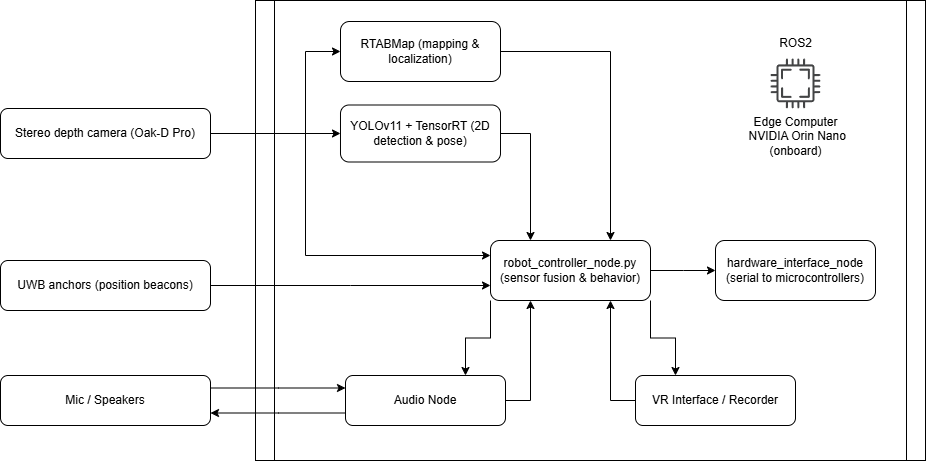
\includegraphics[width=0.85\linewidth]{Images/system_architecture.png}
	\caption{High-level system architecture for Tino V2.}\label{fig-system-architecture}
\end{figure}

\subsection*{Why RTABMap over ORB‑SLAM3 and SVO}
RTABMap provides robust multi-session map persistence, reliable relocalization and first-class ROS/ROS2 integration. During early experiments ORB‑SLAM3 and SVO presented compilation fragility on ARM64 and unstable atlas save/load behavior with the available cameras. RTABMap demonstrated stable map saving/loading and dependable relocalization in practice, making it preferable for a system where map reuse and long-term experiments are required.

\subsection*{Why Stereo Cameras and Oak‑D Pro}
Stereo cameras were selected over both monocular cameras and structured light depth sensors as the primary depth sensing technology due to their fundamental advantages for mobile social robotics applications. Compared to monocular cameras, stereo vision provides direct metric depth estimation without requiring additional sensors or complex monocular depth estimation algorithms that often lack the accuracy needed for precise 3D human pose reconstruction. While monocular depth estimation using neural networks has advanced significantly, it still suffers from scale ambiguity and reduced accuracy at varying distances, making it unsuitable for the metric precision required by VR applications.

Unlike structured light cameras that require active infrared pattern projection, stereo cameras operate passively using ambient light, making them more suitable for continuous operation while the robot is moving without concerns about power consumption from active illumination. Stereo vision also provides more robust depth estimation at varying distances, particularly important for human pose estimation where subjects may be at different ranges from the robot during social interactions.

Additionally, stereo cameras avoid the safety concerns associated with infrared projection near humans, particularly important for a social robot designed to interact closely with people in indoor environments. The passive nature of stereo vision also eliminates potential interference with other infrared devices commonly found in indoor settings, such as remote controls, infrared sensors, or other electronic equipment.

The Oak‑D Pro specifically was chosen because it provides high-quality synchronized stereo depth computation with on‑device processing capabilities, reducing computational load on the main system. The camera integrates well with the DepthAI stack and ROS2 wrappers, demonstrated reliable performance in mapping scenarios, and provided the accurate stereo depth measurements required to convert 2D pose detections into metric 3D joint positions for VR representation.

\subsection*{Why UWB}
UWB anchors provide absolute positioning that compensates SLAM drift and long‑run integration error. When fused with visual SLAM, UWB supplies global corrections and increases robustness in feature‑poor or dynamic areas where visual relocalization is unreliable.

\subsection*{Why YOLOv11 + TensorRT}
YOLOv11, converted to TensorRT engines, provided the best trade-off between detection accuracy and inference throughput on the Orin Nano. The pipeline was extended to extract 17-joint skeletons and fuse per-joint depth from the Oak‑D stereo stream to produce metric 3D skeletons suitable for VR avatars.

\subsection*{R\&D chronology and selection summary}
During development multiple SLAM and VO approaches were evaluated. ORB‑SLAM3 was tested first for its academic strengths and multi‑sensor support, but proved fragile to compile and unstable with the available cameras on ARM64. SVO was attempted as a lighter‑weight alternative but exhibited similar portability and map‑management limitations. RTABMap paired with the Oak‑D Pro ultimately provided the reliable map persistence, dependable relocalization and ROS2 interoperability required for repeated experimentation, and was therefore adopted as the primary mapping solution for Tino V2.

\section{Hybrid localization strategy}

The localization architecture is intentionally hybrid: RTABMap supplies dense map information and orientation (visual odometry and loop closures) while UWB supplies absolute position corrections. The approach follows an architecture with three functional layers:

\begin{enumerate}
	\item \textbf{Sensor acquisition layer:} Oak‑D stereo frames, depth images, RTABMap odometry, UWB range fixes, and IMU measurements are published on ROS2 topics.
	\item \textbf{Local estimation layer:} RTABMap performs visual odometry and graph optimization, producing local pose estimates and maps. Short-term pose updates come from visual odometry and IMU fusion where available.
	\item \textbf{Global fusion layer:} a fusion node ingests RTABMap pose and UWB positions and performs simple sensor selection logic that maintains a consistent global pose used by the rest of the system (VR exporter, motion controller, logging).
\end{enumerate}

This structure leverages RTABMap's strength in building and maintaining appearance-based maps and UWB's absolute fixes to constrain long-term drift. In the Tino V2 implementation the global fusion logic is implemented inside the \texttt{robot\_controller\_node}: it ingests RTABMap poses, UWB fixes, IMU deltas and performs simple sensor selection and fallback logic before publishing the consolidated \texttt{localization\_pose} topic consumed by the VR bridge and other consumers. The detailed sensor fusion architecture and data flow is visualized in Figure~\ref{fig-sensor-fusion}.

\begin{figure}[H]
	\centering
	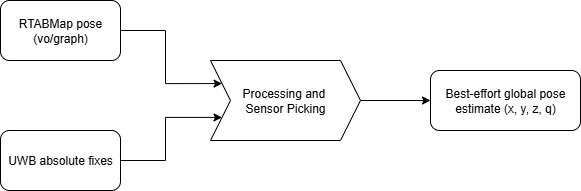
\includegraphics[width=0.85\linewidth]{Images/sensor_fusion.png}
	\caption{Sensor selection and dataflow.}\label{fig-sensor-fusion}
\end{figure}

\subsection*{Sensor fusion contract}
\begin{description}
	\item[Inputs:] RTABMap pose (x, y, z, q), UWB position fixes (x, y, timestamp), IMU measurements (angular velocity, linear acceleration). All inputs are timestamped and published on ROS2 topics.
	\item[Outputs:] A best-effort global pose estimate (x, y, z, q) selected from available sensors; the node republishes the fused pose at a variable rate (typically 10--50\,Hz depending on sensor availability and computational load).
	\item[Error modes:] \begin{itemize}[nosep,leftmargin=*]
		\item \textbf{Missing UWB fixes:} the fusion falls back to visual odometry from RTABMap.
		\item \textbf{Visual tracking loss:} the system holds the last known map pose and uses UWB position with estimated orientation from movement direction; if unsuccessful, it raises an operator-visible warning.
		\item \textbf{Inconsistent UWB readings:} basic validity checks are applied and the system falls back to RTABMap position when UWB appears invalid.
	\end{itemize}
\end{description}

\subsection*{Edge cases and mitigations}
The hybrid localization system must handle several challenging scenarios that can compromise positioning accuracy. Each edge case requires specific detection mechanisms and fallback strategies to maintain system reliability:

\begin{itemize}
	\item \textbf{NLOS UWB measurements:} Non-Line-of-Sight (NLOS) conditions occur when UWB signals reflect off walls or furniture before reaching anchors, causing distance measurements to be longer than the true direct path. This leads to positioning errors that can be several meters off the robot's actual location. The system detects NLOS conditions by comparing UWB-derived positions against RTABMap's visual estimates and checking for sudden position jumps that exceed physically possible robot movement speeds. When NLOS is detected, the fusion logic temporarily ignores UWB fixes and relies solely on RTABMap's visual odometry until consecutive UWB measurements show consistent, physically plausible positions again.
	
	\item \textbf{Feature-poor areas (e.g., blank walls):} Visual SLAM systems like RTABMap require sufficient visual features (corners, textures, patterns) to track camera motion and maintain localization. In environments with blank walls, uniform lighting, or repetitive patterns, the camera may lose tracking or produce unreliable odometry estimates. When RTABMap loses tracking, the system automatically triggers relocalization attempts and informs the VR operator that tracking has been lost and relocalization is in progress. The system relies on the VR user to continue moving the robot (particularly rotating in place) to provide RTABMap with sufficient visual motion to reacquire its position within the existing map. Since UWB typically maintains position estimates, orientation recovery is the primary challenge in these scenarios.
	
	\item \textbf{Camera occlusion by robot fabric:} The Tino robot's fabric covering can occasionally shift during movement and partially obstruct the Oak-D Pro camera's field of view, particularly during rapid rotations or when interacting with humans. This occlusion degrades both RGB image quality for human pose detection and stereo depth estimation reliability. Typically, these occlusion events are brief moments where the fabric temporarily covers the camera before settling back into position, but even these short disruptions can trigger RTABMap relocalization attempts. Currently, the system does not automatically detect or respond to fabric occlusion events - this remains a manual intervention scenario where operators must physically adjust the robot's fabric covering to restore clear camera views when persistent occlusion occurs.
\end{itemize}

\section{Human detection and pose pipeline}

The human perception pipeline is designed to provide real-time 3D skeletons to the VR environment and other behavior nodes. It consists of three stages:

\begin{enumerate}
	\item \textbf{2D detection and pose estimation:} YOLOv11 (TensorRT engine) runs on RGB frames to detect humans and estimate 2D keypoints (17 joints).
	\item \textbf{Depth association:} for each detected joint, the pipeline samples the Oak‑D stereo depth (with median filtering in a small neighbourhood) to recover the joint's metric z coordinate and compute the (x,y,z) position in the camera frame.
	\item \textbf{Transform to robot/world frame:} the 3D joint positions are transformed using the current fused global pose to provide world-relative skeleton's coordinates for VR and navigation.
\end{enumerate}

This multi-stage processing pipeline, from initial RGB input through 2D pose detection to final 3D skeleton output, is illustrated in Figure~\ref{fig-human-pipeline}.

\begin{figure}[H]
	\centering
	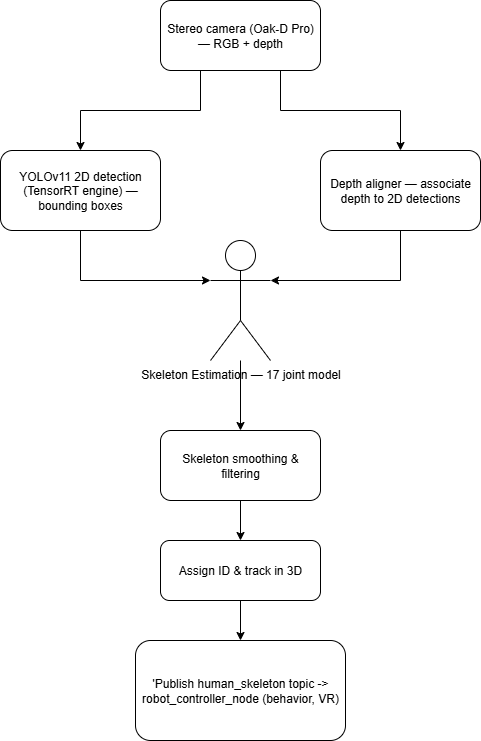
\includegraphics[height=12cm]{Images/human_pipeline.png}
	\caption{Human detection and depth-association pipeline.}\label{fig-human-pipeline}
\end{figure}

The pipeline publishes a \texttt{human\_skeleton} ROS2 message containing a timestamped array of joints, each with position and a confidence score. This message enables downstream nodes to select stable skeletons for interaction logic and VR rendering.

\subsection*{Design contract for perception}
Inputs: synchronized RGB frame, depth image, camera intrinsics, current global pose.
Outputs: timestamped skeletons with 3D joint positions and per-joint confidence.
Failure modes: low confidence joints (reported but flagged), missing depth (use last known depth or drop joint), multiple detections (assign IDs using bounding-box IoU + temporal tracking).

\section{Software architecture and system organisation}

To improve modularity and maintainability the entire robot stack was migrated to ROS2. The project uses a node-based split that mirrors the functional decomposition:

\begin{itemize}
	\item \textbf{Perception:} \texttt{rtabmap} (mapping/localization), \texttt{depthai} camera node, \texttt{yolo11\_pose\_node} (TensorRT inference + skeleton extraction).
	\item \textbf{State and logging:} \texttt{vr\_data\_recorder\_node} (logging for VR and experiments).
	\item \textbf{Control (includes fusion):} \texttt{robot\_controller\_node.py} implements simple sensor selection logic (UWB preferred for position, RTABMap for orientation) and high-level behaviours; \texttt{hardware\_interface\_node.py} handles serial comms to Arduinos using device symlinks \texttt{/dev/ttyHEAD}, \texttt{/dev/ttyBASE}, \texttt{/dev/ttyLEG}.
	\item \textbf{I/O and integration:} \texttt{gamepad\_node.py}, \texttt{audio\_node.py}, \texttt{vr\_interface\_node.py} (VR bridge and topic translation).
\end{itemize}

Design decisions that improved robustness during development included using persistent device symlinks for Arduinos, clearly separated launch files for mapping and localization (\texttt{rtab\_mapping.launch.py}, \texttt{rtab\_localization.launch.py}), and a dedicated VR exporter node that limits published bandwidth and enforces message rate caps for stable VR telepresence.

\section{Implementation notes and rationale from R\&D}

Several practical findings from the development period informed the conceptual choices:

\begin{itemize}
	\item ORB‑SLAM3 and SVO showed compilation and stability problems on ARM64 devices and with older RealSense/T265 hardware; this motivated the switch to RTABMap and the Oak‑D Pro camera.
	\item The Oak‑D Pro + RTABMap standalone build achieved reliable map save/load and relocalization, a key requirement for repeated VR sessions.
	\item Converting YOLOv11 to TensorRT produced the necessary runtime performance for 17-joint skeleton extraction on the Orin Nano while keeping end-to-end latency acceptable for virtual reality.
	\item Power architecture and mechanical changes (new differential base, improved mounts for camera and speakers) reduced vibration and improved perception robustness in the field.
\end{itemize}

\section{Validation plan and quality gates}

To verify the conceptual choices and measure system readiness the following minimal quality gates were defined and executed where possible:

\begin{enumerate}
	\item \textbf{Build and integration:} RTABMap + DepthAI + ROS2 launch files must start and publish \texttt{localization\_pose} and camera topics without crashes for 10 minutes (smoke test).
	\item \textbf{Perception correctness:} YOLOv11 TensorRT skeletons validated against recorded test sequences; per-joint reprojection error to depth must be within 20 cm for frontal poses.
	\item \textbf{Fusion stability:} sensor selection logic must provide reasonable pose estimates when UWB anchors are available, and be able to relocalize to saved maps.
	\item \textbf{End-to-end latency:} perception -> VR message latency measured and kept below 150 ms in typical configurations.
\end{enumerate}

Measured results from the R\&D include:
\begin{itemize}[nosep]
	\item RTABMap with Oak‑D saved and reloaded maps reliably.
	\item YOLOv11 (TensorRT) provided real-time skeletons suitable for VR export.
	\item Orin Nano peak current draw was measured and verified as acceptable after power supply revisions.
\end{itemize}

\section{Summary}

The conceptual framework presented in this chapter establishes the foundation for Tino V2's technical implementation, with each technology choice validated through practical development experience and performance requirements for VR integration.



% Chapter 4: Implementation
\chapter{Implementation}
\section{Hardware Platform Migration and Integration}
This section will detail the complete hardware migration from the legacy Raspberry Pi system to the modern NVIDIA Orin Nano platform and the integration of new sensing technologies. The computing platform upgrade will be presented first, covering the migration process from Raspberry Pi 4 to NVIDIA Orin Nano including performance benchmarking that demonstrated substantial improvements in processing capability, the power system redesign using DC-DC converters to provide stable 19V power for the Orin Nano from 12V battery systems, and the cooling and thermal management solutions implemented to ensure reliable operation during intensive computational tasks. The camera system integration will be detailed, covering the replacement of the basic Pi camera with the Oak-D Pro depth camera system, the mechanical mounting solutions developed including the tripod-based camera support system and protective housing that shields the camera while maintaining visibility, and the camera calibration procedures required for accurate depth estimation and SLAM performance. The UWB positioning system implementation will be examined, covering the anchor placement strategy developed for the laboratory environment, the coordinate system calibration procedures that align UWB global coordinates with the robot's local reference frame, and the integration of UWB receivers with the Orin Nano through USB interfaces and custom ROS2 drivers. The mechanical system upgrades will be addressed, covering the complete redesign of the base locomotion system from omnidirectional triksta wheels to differential drive configuration, the motor and driver upgrades that provide increased power and reliability for the heavier Orin Nano system, and the Stewart platform head improvements including new arm designs with heim joints that eliminate flex and improve reliability.

\section{ROS2 Software Architecture Implementation}
This section will present the complete implementation of the ROS2-based software architecture that replaced the legacy monolithic Python scripts with a modular, maintainable system. The node architecture design will be established first, covering the development of specialized ROS2 nodes including gamepad\_node.py for Xbox controller input processing, hardware\_interface\_node.py for Arduino communication management, robot\_controller\_node.py for central coordination and behavior management, and vr\_interface\_node.py for Unity integration and data exchange. The communication framework implementation will be detailed, covering the ROS2 topic structure that enables real-time data sharing between nodes, the service interfaces used for system configuration and control commands, the parameter management system that allows runtime configuration of system behavior, and the launch file organization that enables easy switching between mapping and localization operational modes. The Arduino integration will be examined, covering the serial communication protocols developed for reliable data exchange with head, base, and leg control systems, the device symlink configuration that ensures consistent device addressing across system restarts, and the command processing logic that translates high-level movement commands into appropriate motor control signals. The data recording and analysis infrastructure will be presented, covering the implementation of comprehensive logging systems that capture all sensor data, robot states, and user interactions for later analysis, the data extraction tools developed for processing recorded sessions, and the visualization systems that enable real-time monitoring of system performance and debugging of operational issues.

\section{SLAM and Sensor Fusion Implementation}
This section will detail the implementation of the RTABMap SLAM system and its integration with UWB positioning for robust indoor localization. The RTABMap configuration and optimization will be presented first, covering the parameter tuning process that optimized performance for the Oak-D Pro camera system, the memory management configuration that enables long-term mapping without excessive resource consumption, and the loop closure detection settings that ensure reliable map consistency during extended operation. The UWB integration implementation will be detailed, covering the development of custom ROS2 nodes for UWB data processing and coordinate transformation, the sensor fusion logic that combines UWB position data with RTABMap orientation information, and the coordinate system alignment procedures that ensure consistent mapping between UWB global coordinates and robot local coordinates. The mapping and localization modes will be examined, covering the implementation of distinct operational modes for initial map creation and subsequent localization within existing maps, the map saving and loading procedures that enable persistent environment representations, and the automatic relocalization capabilities that allow the robot to recover its position after temporary tracking loss. The performance optimization will be addressed, covering the computational optimization that enables real-time SLAM processing on the Orin Nano platform, the memory management strategies that prevent performance degradation during extended mapping sessions, and the error handling procedures that maintain system stability when sensor data is temporarily unavailable or degraded.

\section{Human Detection and Pose Estimation Implementation}
This section will present the implementation of real-time human detection and pose estimation using YOLOv11 with TensorRT optimization. The YOLOv11 model preparation and optimization will be detailed first, covering the conversion process from PyTorch models to TensorRT optimized engines for the Orin Nano platform, the model quantization and optimization strategies that balance detection accuracy with inference speed, and the integration with the Oak-D Pro camera system that enables simultaneous RGB and depth data processing for 3D pose estimation. The real-time processing pipeline will be examined, covering the image preprocessing and postprocessing steps that prepare camera data for inference and extract meaningful pose information, the coordinate transformation calculations that convert 2D detection results to 3D world coordinates using depth information, and the tracking algorithms that maintain consistent person identification across multiple frames. The pose estimation implementation will be detailed, covering the 17-keypoint skeleton detection that provides comprehensive human pose information, the depth integration that enables accurate 3D position calculation for each detected person, and the filtering and smoothing algorithms that reduce noise and provide stable pose tracking despite occasional detection errors. The integration with robot systems will be addressed, covering the ROS2 message structures used to publish human detection and pose data for use by other system components, the coordinate system transformations that align human pose data with robot and world coordinate frames, and the performance monitoring systems that track detection accuracy and computational load to ensure real-time operation requirements are maintained.

\section{VR Integration and Atomic Movement System Implementation}
This section will detail the implementation of the complete VR integration system including Unity-based user interfaces and atomic movement control architecture. The Unity VR application development will be presented first, covering the creation of immersive VR environments that provide intuitive robot control interfaces, the implementation of bidirectional communication systems that enable real-time data exchange between Unity and ROS2, and the user interface design that makes robot control accessible to users without technical expertise. The ROS-TCP-Endpoint integration will be examined, covering the implementation of reliable communication bridges between Unity and the ROS2 ecosystem, the message serialization and deserialization procedures that handle complex data structures, and the error handling and reconnection logic that maintains communication stability despite network interruptions. The atomic movement system implementation will be detailed, covering the four-state control architecture implemented in both leg and base controllers, the synchronization mechanisms that ensure coordinated movement between robot subsystems, and the command queuing and locking systems that prevent conflicting movement commands. The audio system integration will be addressed, covering the implementation of bidirectional audio communication that enables natural conversation between VR users and people near the robot, the audio processing pipelines that handle microphone input and speaker output, and the integration with the VR system that provides seamless audio transmission. The data recording and analysis implementation will be presented, covering the comprehensive logging systems that capture all VR interactions, robot responses, and sensor data for detailed analysis of human-robot interaction patterns, the data extraction and visualization tools that enable researchers to analyze user behavior and system performance, and the real-time monitoring systems that provide immediate feedback about system operation and performance metrics during VR sessions.

\section{System Integration and Testing Infrastructure}
This section will present the implementation of comprehensive system integration procedures and testing infrastructure that ensure reliable operation of all system components. The integration testing methodology will be established, covering the systematic approach used to validate individual subsystem functionality before full system integration, the interface testing procedures that verify reliable communication between ROS2 nodes, and the end-to-end testing protocols that validate complete system operation from VR input to robot response. The calibration and configuration management will be detailed, covering the sensor calibration procedures required for accurate camera, UWB, and coordinate system alignment, the parameter management systems that store and maintain optimal configuration settings for different operational scenarios, and the automated configuration validation tools that detect and report configuration errors or drift. The debugging and monitoring infrastructure will be examined, covering the comprehensive logging systems that capture detailed system state information for troubleshooting and optimization, the real-time monitoring displays that provide immediate feedback about system performance and health, and the automated error detection and reporting systems that identify and classify system issues to support rapid problem resolution. The deployment and maintenance procedures will be addressed, covering the automated setup scripts that streamline system installation and configuration, the backup and recovery procedures that protect against data loss and enable rapid system restoration, and the update and maintenance protocols that enable safe system modification and capability enhancement without disrupting ongoing research activities.


\section{Hardware Implementation}
\label{sec:hardware_impl}

% REORG_TAG: moved here from Kinematic Base Upgrade from Omnidirectional to Differential Drive
\subsection{Kinematic Base Redesign}

Extended operational testing of Tino's original omnidirectional Triskar base revealed systematic mechanical failures and control complexities that threatened system reliability during social interaction research. The three-wheel omnidirectional configuration, initially selected for maximum maneuverability, proved unsuitable for Tino's 20kg operational weight and predominantly forward-motion interaction patterns.

\subsubsection{System Failure Analysis and Design Requirements}

The original Triskar platform exhibited multiple failure modes under operational demands. Omniwheel rollers experienced systematic deformation, with surfaces becoming squared due to continuous plastic deformation under Tino's weight, creating irregular rolling characteristics that manifested as vibration, reduced traction, and unpredictable movement behavior. Roller bearing failures occurred frequently in the rear omniwheel due to dragging forces during movement operations, while the three-wheel configuration created uneven weight distribution with the rear wheel experiencing excessive drag forces that accelerated component wear.

\begin{figure}[H]
    \centering
    \includegraphics[width=0.5\textwidth]{Images/wire_triskar.png}
    \caption{Original Triskar Base System}
    \label{fig:original_Triskar_base}
\end{figure}

Motor performance analysis revealed inadequate torque delivery under sustained loading, with heating issues during extended use leading to performance degradation. The omnidirectional kinematics required sophisticated coordination between three drive motors while compensating for mechanical variability, creating control system complexity. Additionally, dependency on the VirHas library limited customization capabilities and created maintenance challenges for the Tino platform's specific requirements.

\subsubsection{Differential Drive Solution Design}

To address these limitations, a differential drive architecture was selected, prioritizing mechanical simplicity, enhanced reliability, and improved maintainability while providing adequate maneuverability for Tino's social interaction requirements. The design eliminates omnidirectional complexity while maintaining essential mobility through a two-wheel configuration with rear caster support that provides stable platform dynamics with reduced component count.

\begin{figure}[H]
    \centering
    \includegraphics[width=0.7\textwidth]{Images/NewBaseDifferentialDrive.jpg}
    \caption{Complete Differential Drive Base with T-Structure Framework}
    \label{fig:differential_base_complete}
\end{figure}

Weight distribution optimization utilizes the two front drive wheels to support the majority of Tino's operational weight while the rear caster provides stability without bearing significant driving loads, eliminating the dragging forces that compromised the original system. Maneuverability analysis demonstrates that differential drive provides adequate turning capability through differential wheel speed control, with simplified kinematics enabling more precise movement control and improved repeatability. This architecture proved highly effective, providing the reliable mobility foundation necessary for supporting the enhanced computational requirements of the power system upgrade detailed in the following section.

\subsubsection{Mechanical Implementation and System Integration}

The mechanical implementation required comprehensive base reconstruction utilizing aluminum Item profiles to create a robust T-structure framework. This modular profile system provides structural rigidity while enabling mechanical adjustments without complete system redesign, with wheel spacing optimization through the adjustable T-structure enabling fine-tuning of track width to achieve proper balance and stability characteristics.

\begin{figure}[H]
    \centering
    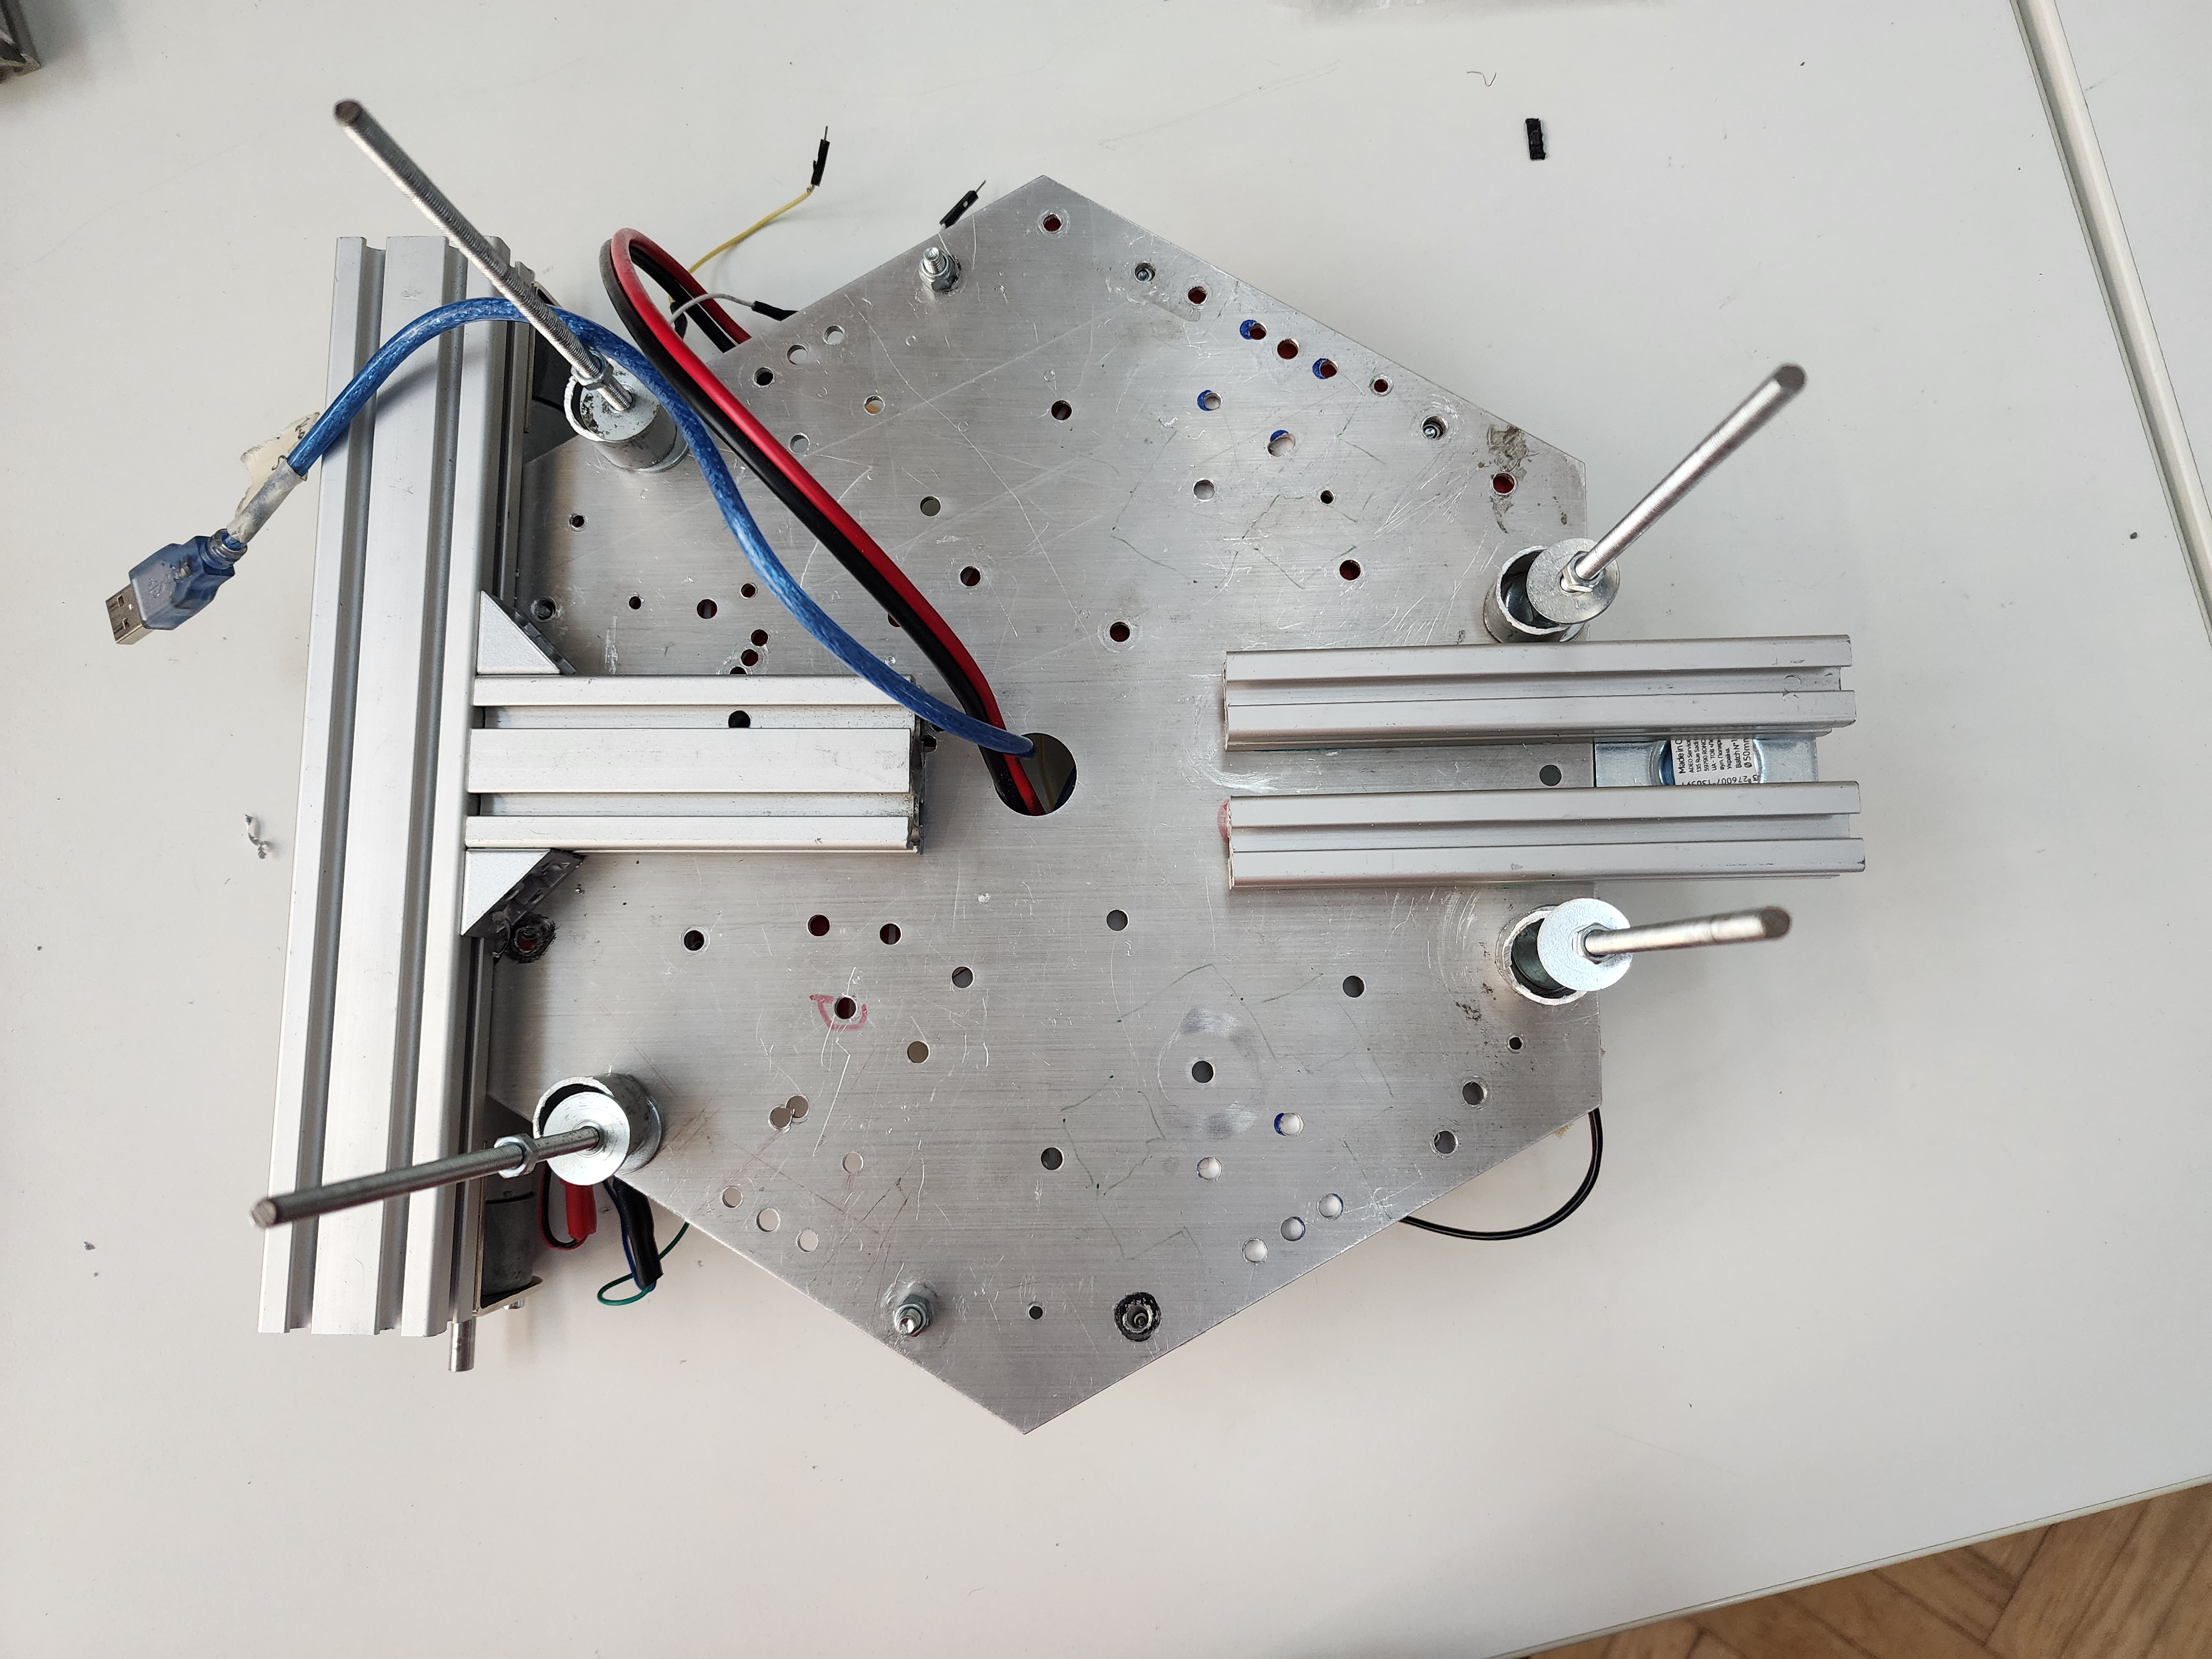
\includegraphics[width=0.6\textwidth]{Images/NewBaseDifferentialDrive (5).jpg}
    \caption{Top View of Differential Drive Base with T-Structure}
    \label{fig:differential_base_top}
\end{figure}

Motor mounting points integrate directly with the Item profile system through custom brackets providing precise alignment and secure attachment. The motor upgrade to more powerful units addresses the thermal and torque limitations of the original system, with new motors providing enhanced heat dissipation capabilities and higher continuous torque ratings suitable for Tino's operational requirements. Motor driver upgrade to the MDD10A units provides increased current handling capability and enhanced control responsiveness compared to the original dual-driver configuration.

\begin{figure}[H]
    \centering
    \begin{minipage}{0.45\textwidth}
        \centering
        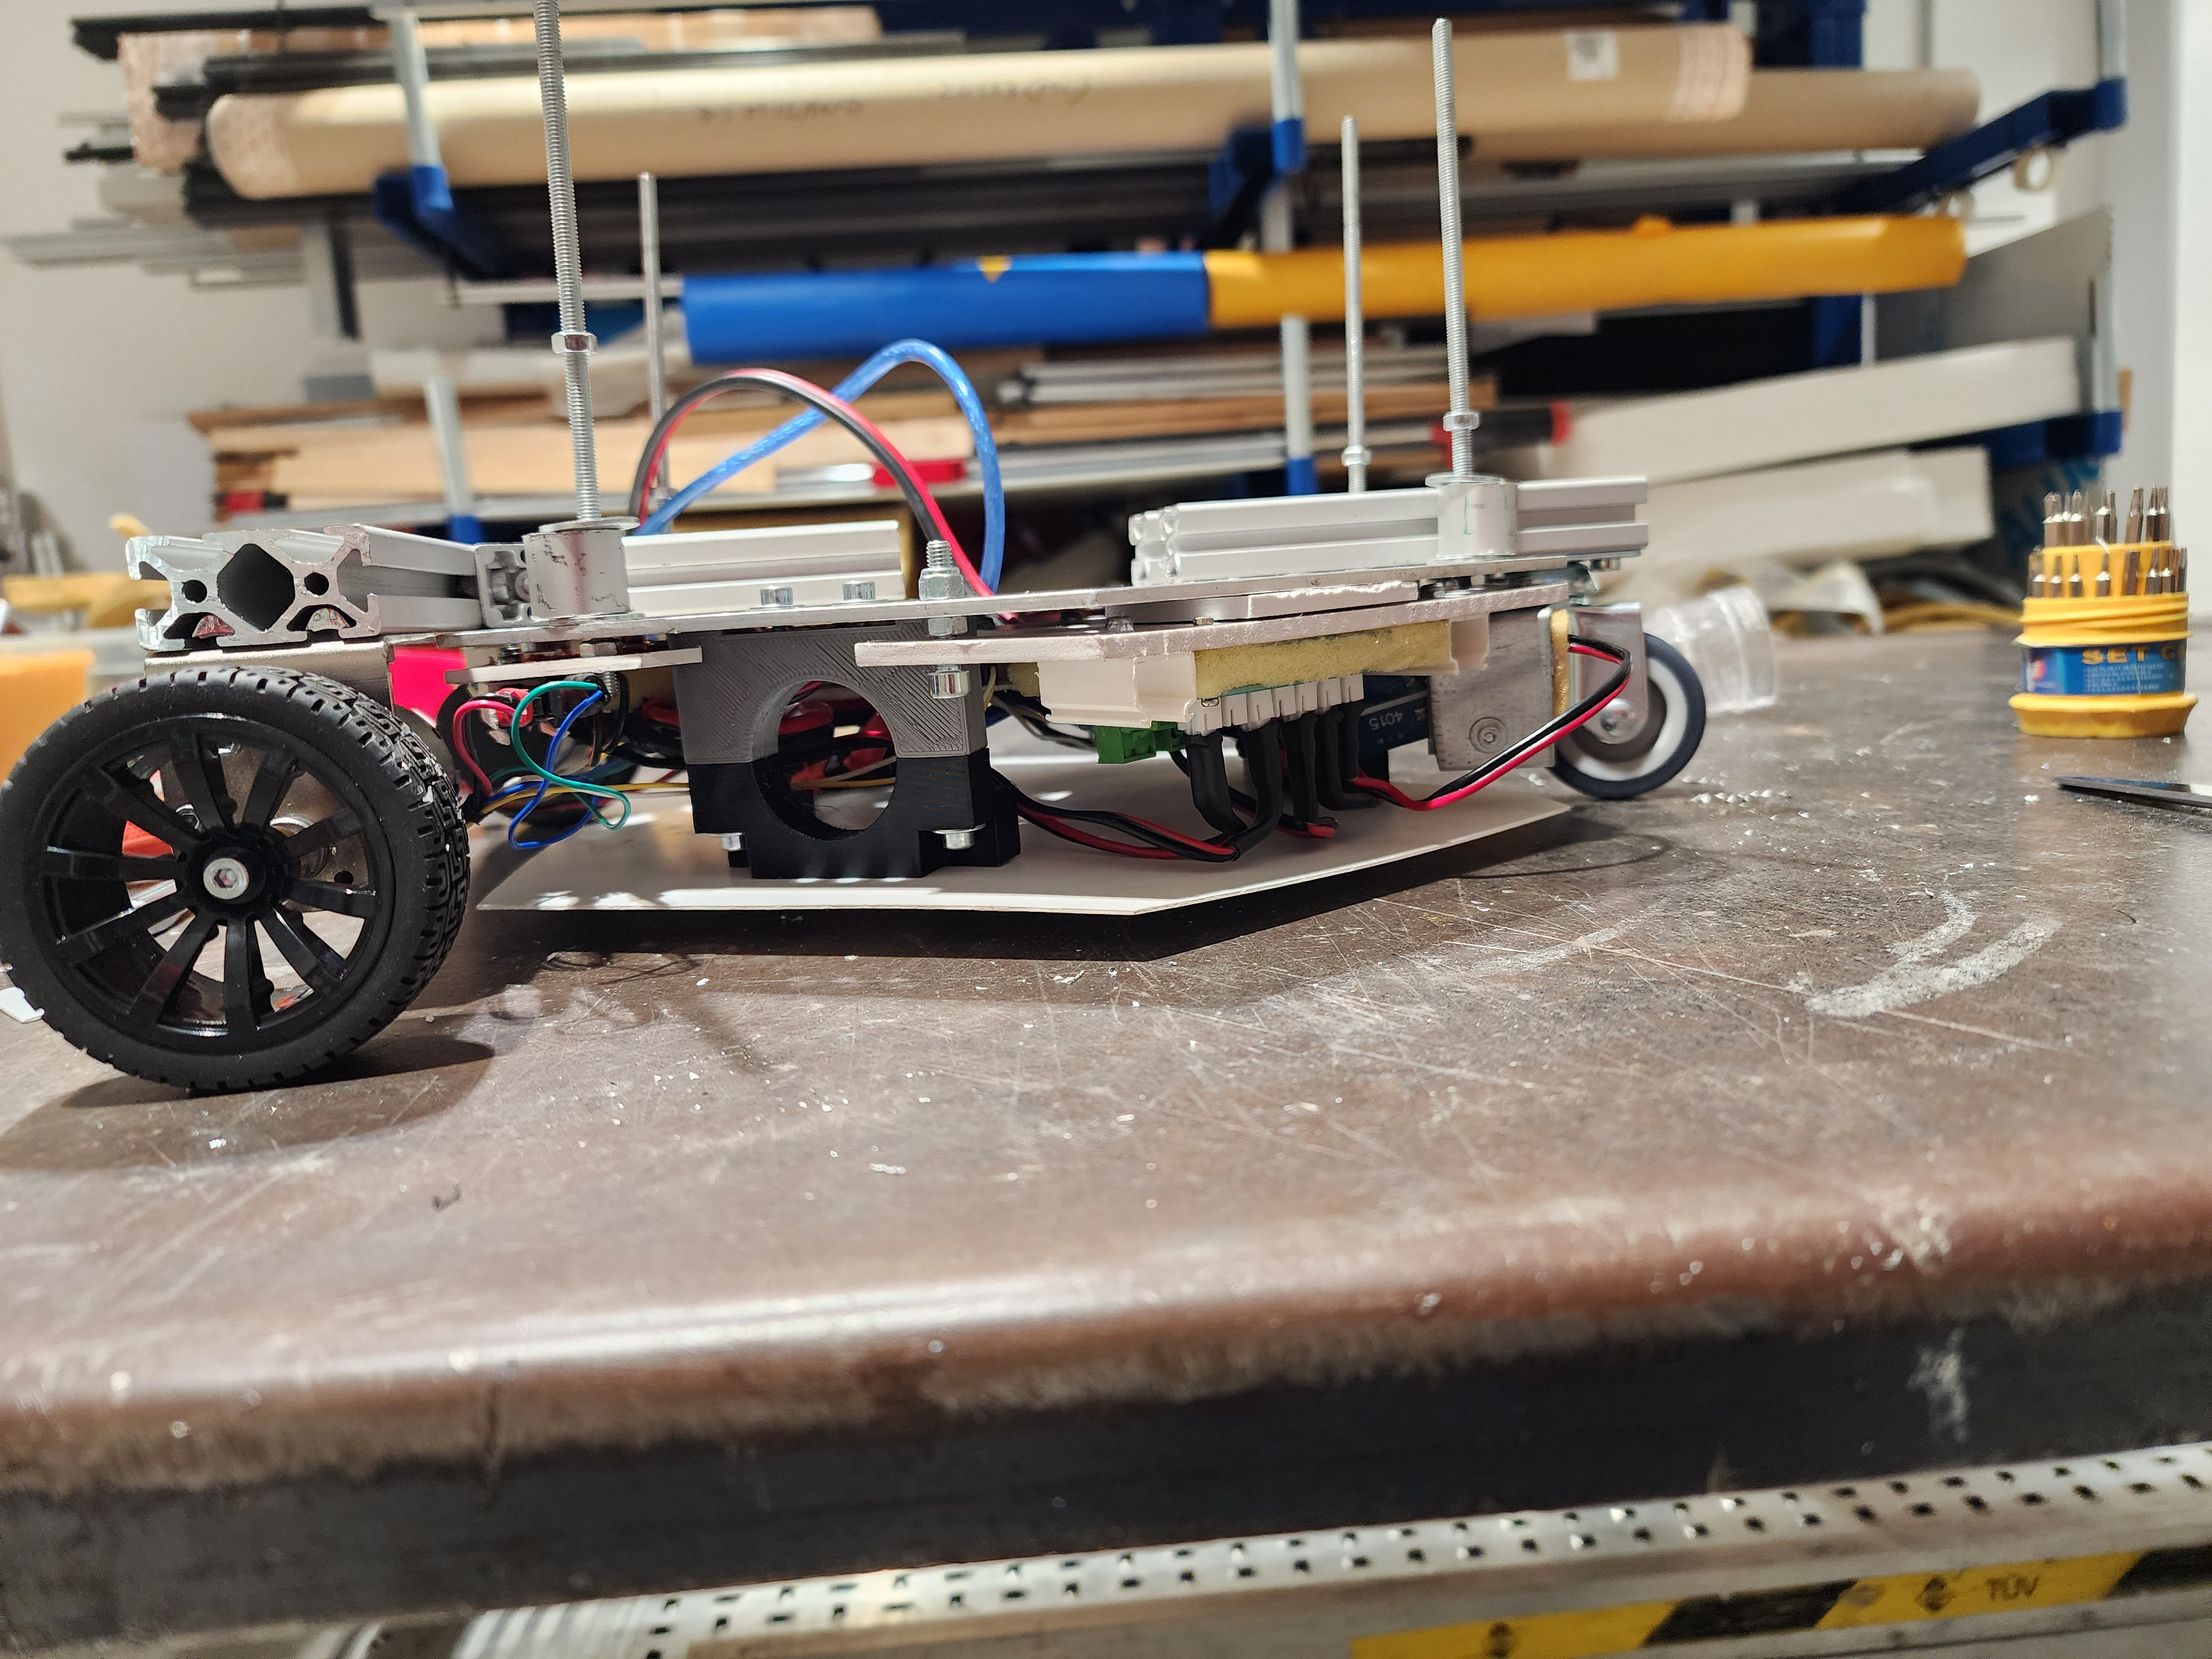
\includegraphics[width=\textwidth]{Images/NewBaseDifferentialDrive (2).jpg}
        \caption{Differential Drive Base Side View}
        \label{fig:differential_base_side}
    \end{minipage}
    \hfill
    \begin{minipage}{0.45\textwidth}
        \centering
        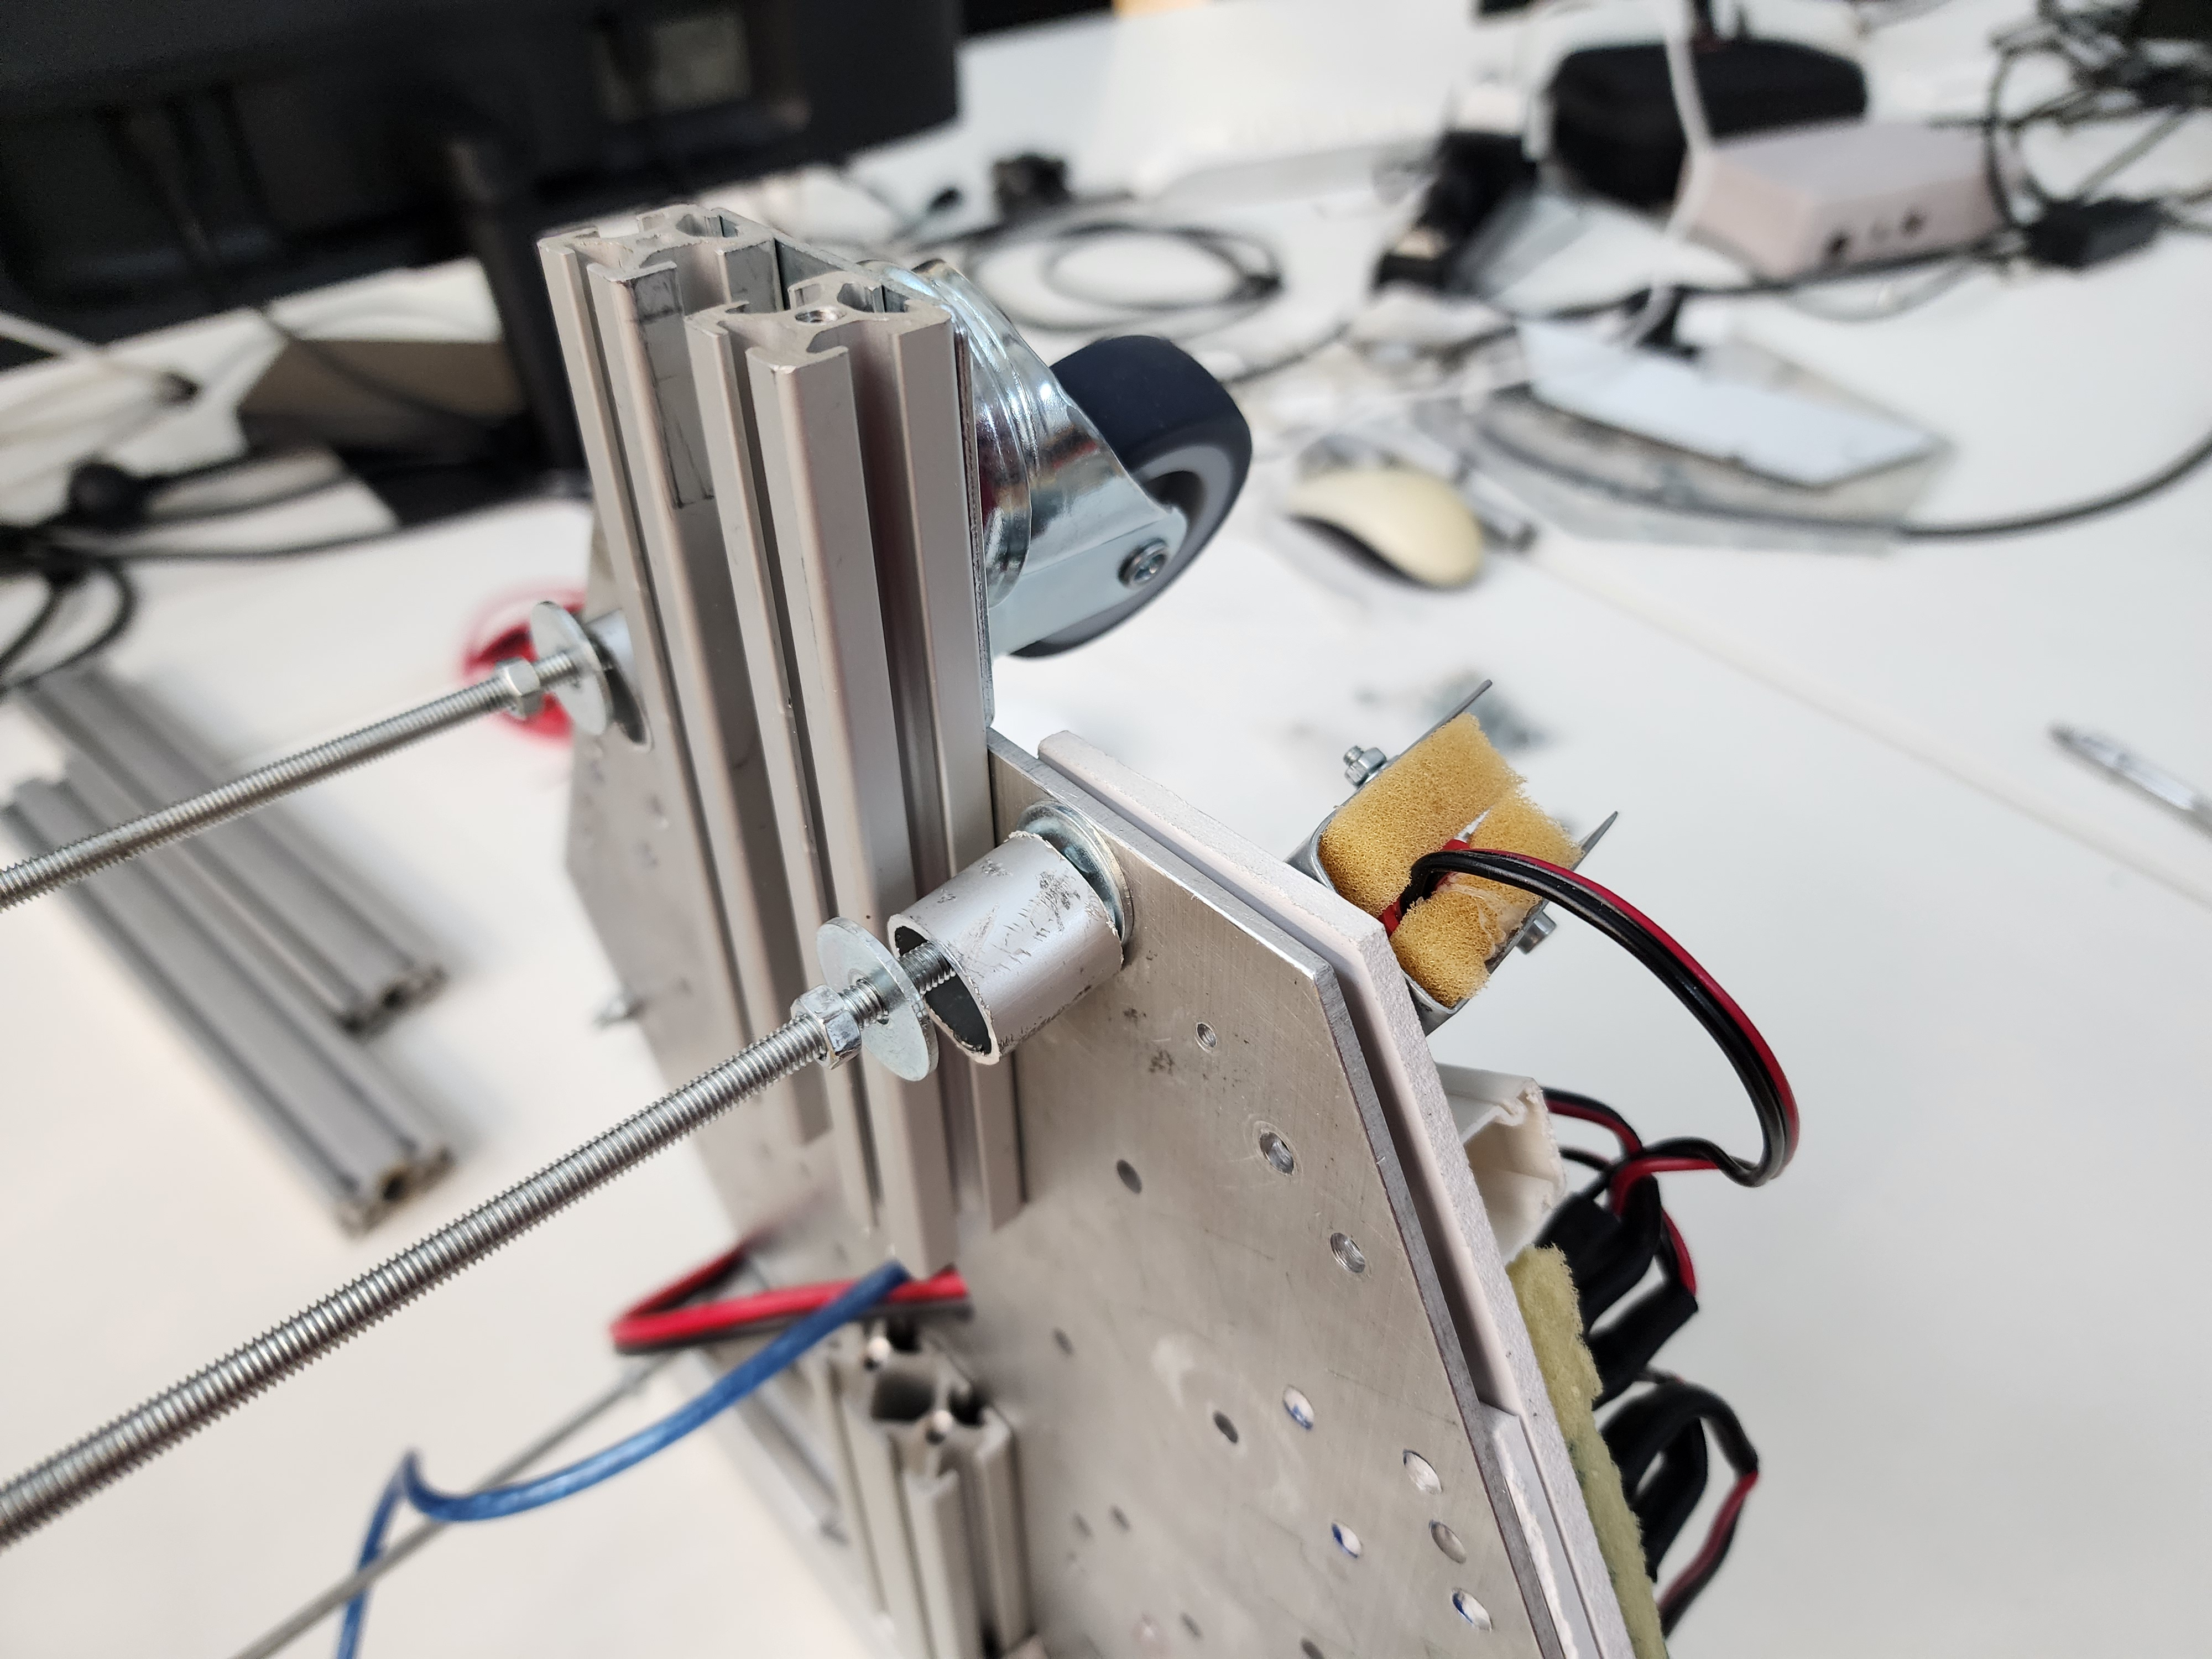
\includegraphics[width=\textwidth]{Images/NewBaseDifferentialDrive (3).jpg}
        \caption{Caster Wheel supporting Rear of Base}
        \label{fig:differential_base_caster}
    \end{minipage}
\end{figure}

\begin{figure}[H]
    \centering
    \begin{minipage}{0.45\textwidth}
        \centering
        \includegraphics[width=\textwidth,angle=-90]{Images/BaseNewMotors.jpg}
        \caption{Base with New Motors (Top View)}
        \label{fig:base_new_motors}
    \end{minipage}
    \hfill
    \begin{minipage}{0.45\textwidth}
        \centering
        \includegraphics[width=\textwidth,angle=-90]{Images/BaseNewMotors2.jpg}
        \caption{Base with New Motors (Close up Side View)}
        \label{fig:base_new_motors_side}
    \end{minipage}
\end{figure}

\subsubsection{Wheel System and Control Integration}

The wheel selection process revealed challenges with plastic hub construction under operational loads, requiring iterative development to achieve reliable traction and durability. Initial plastic wheels with pneumatic rubber tires provided adequate traction but suffered from hub failure and tire debeading issues when rubber separated from plastic hubs due to inadequate bonding strength. The solution involved wheel hub reinforcement through hot-glue filling, which addressed structural weakness while maintaining traction characteristics, though representing a temporary fix requiring future system upgrade.

\begin{figure}[H]
    \centering
    \begin{subfigure}{0.45\textwidth}
        \centering
        \includegraphics[width=\textwidth]{Images/WheelSilicona (3).jpg}
        \caption{Wheel Front View}
        \label{fig:wheel_hotglue}
    \end{subfigure}
    \hfill
    \begin{subfigure}{0.45\textwidth}
        \centering
        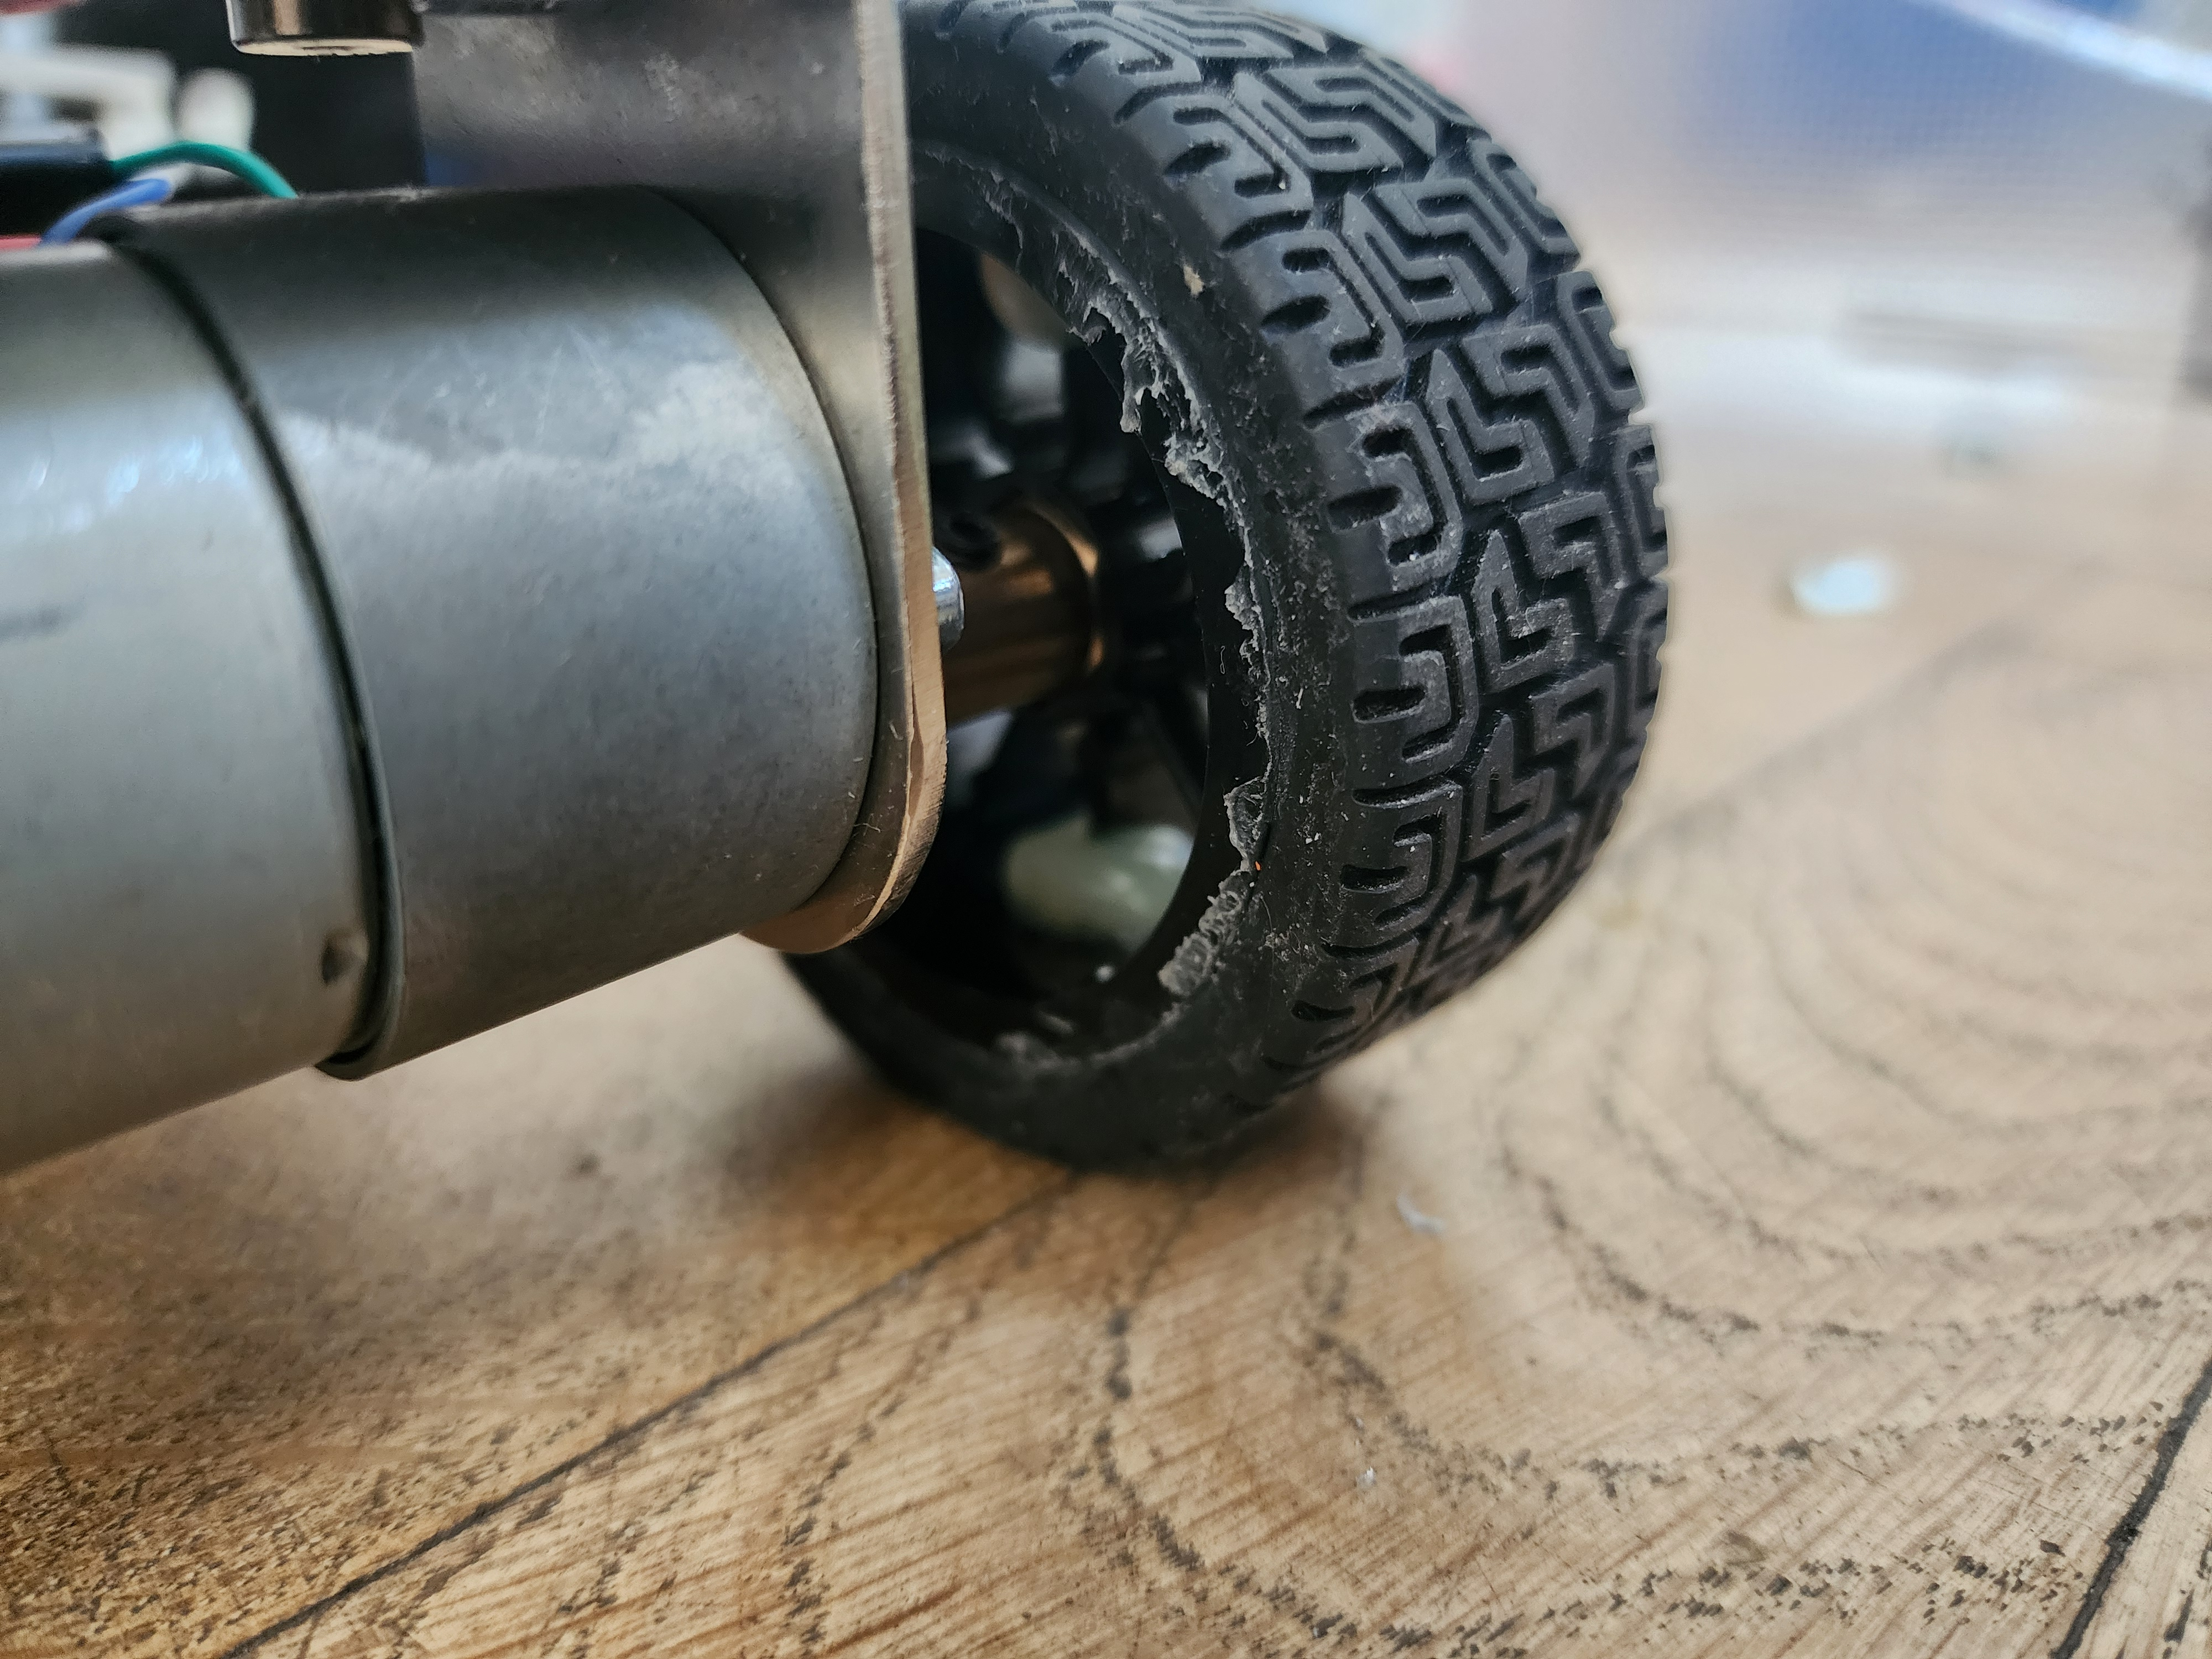
\includegraphics[width=\textwidth]{Images/WheelSilicona.jpg}
        \caption{Wheel Mounted on Motor Shaft}
        \label{fig:wheel_silicone}
    \end{subfigure}
    \caption{Wheel with Hot-Glue Filled Tires}
    \label{fig:combined}
\end{figure}

Fabric interference prevention required protective bumper implementation to prevent Tino's fabric covering from interfering with wheel operation. The bumper design provides physical separation between moving wheels and flexible fabric structure, with effectiveness testing demonstrating successful prevention of fabric entanglement in most operational scenarios.

\begin{figure}[H]
    \centering
    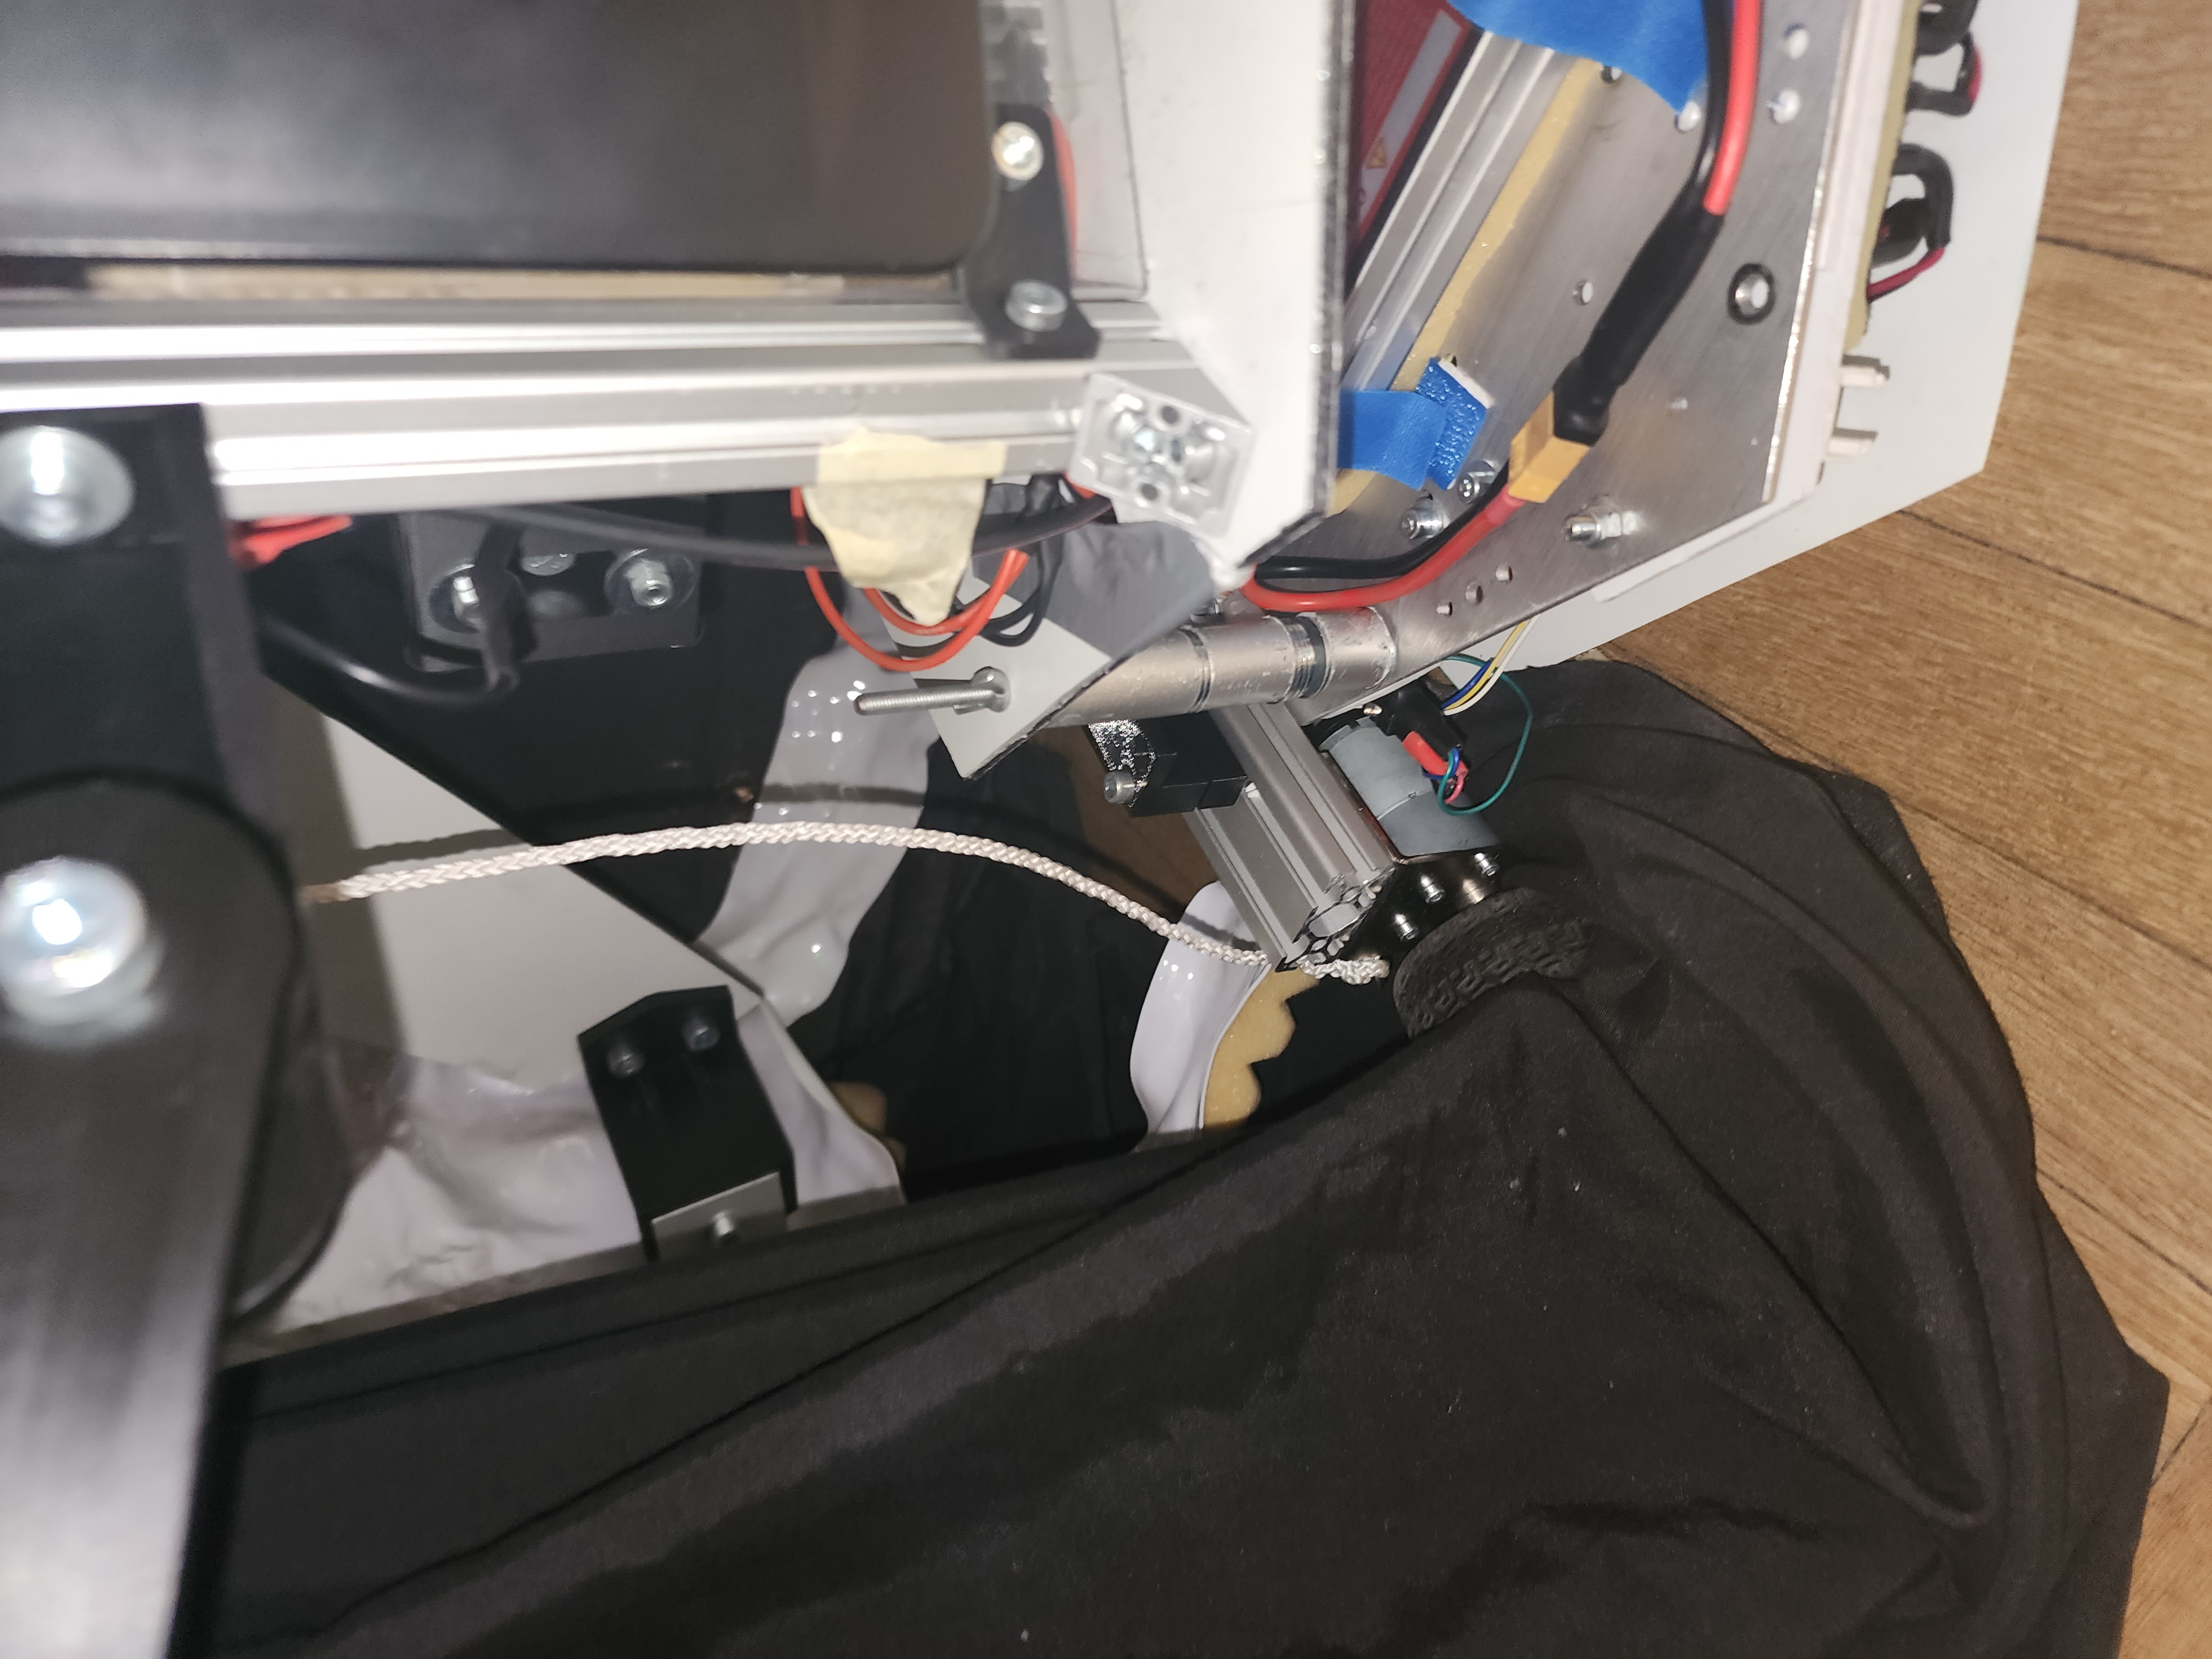
\includegraphics[height=6cm,angle=-90]{Images/WheelVSFabric (2).jpg}
    \caption{Wheel vs Fabric Interference}
    \label{fig:wheel_vs_fabric}
\end{figure}

\begin{figure}[H]
    \centering
    \begin{minipage}{0.45\textwidth}
        \centering
        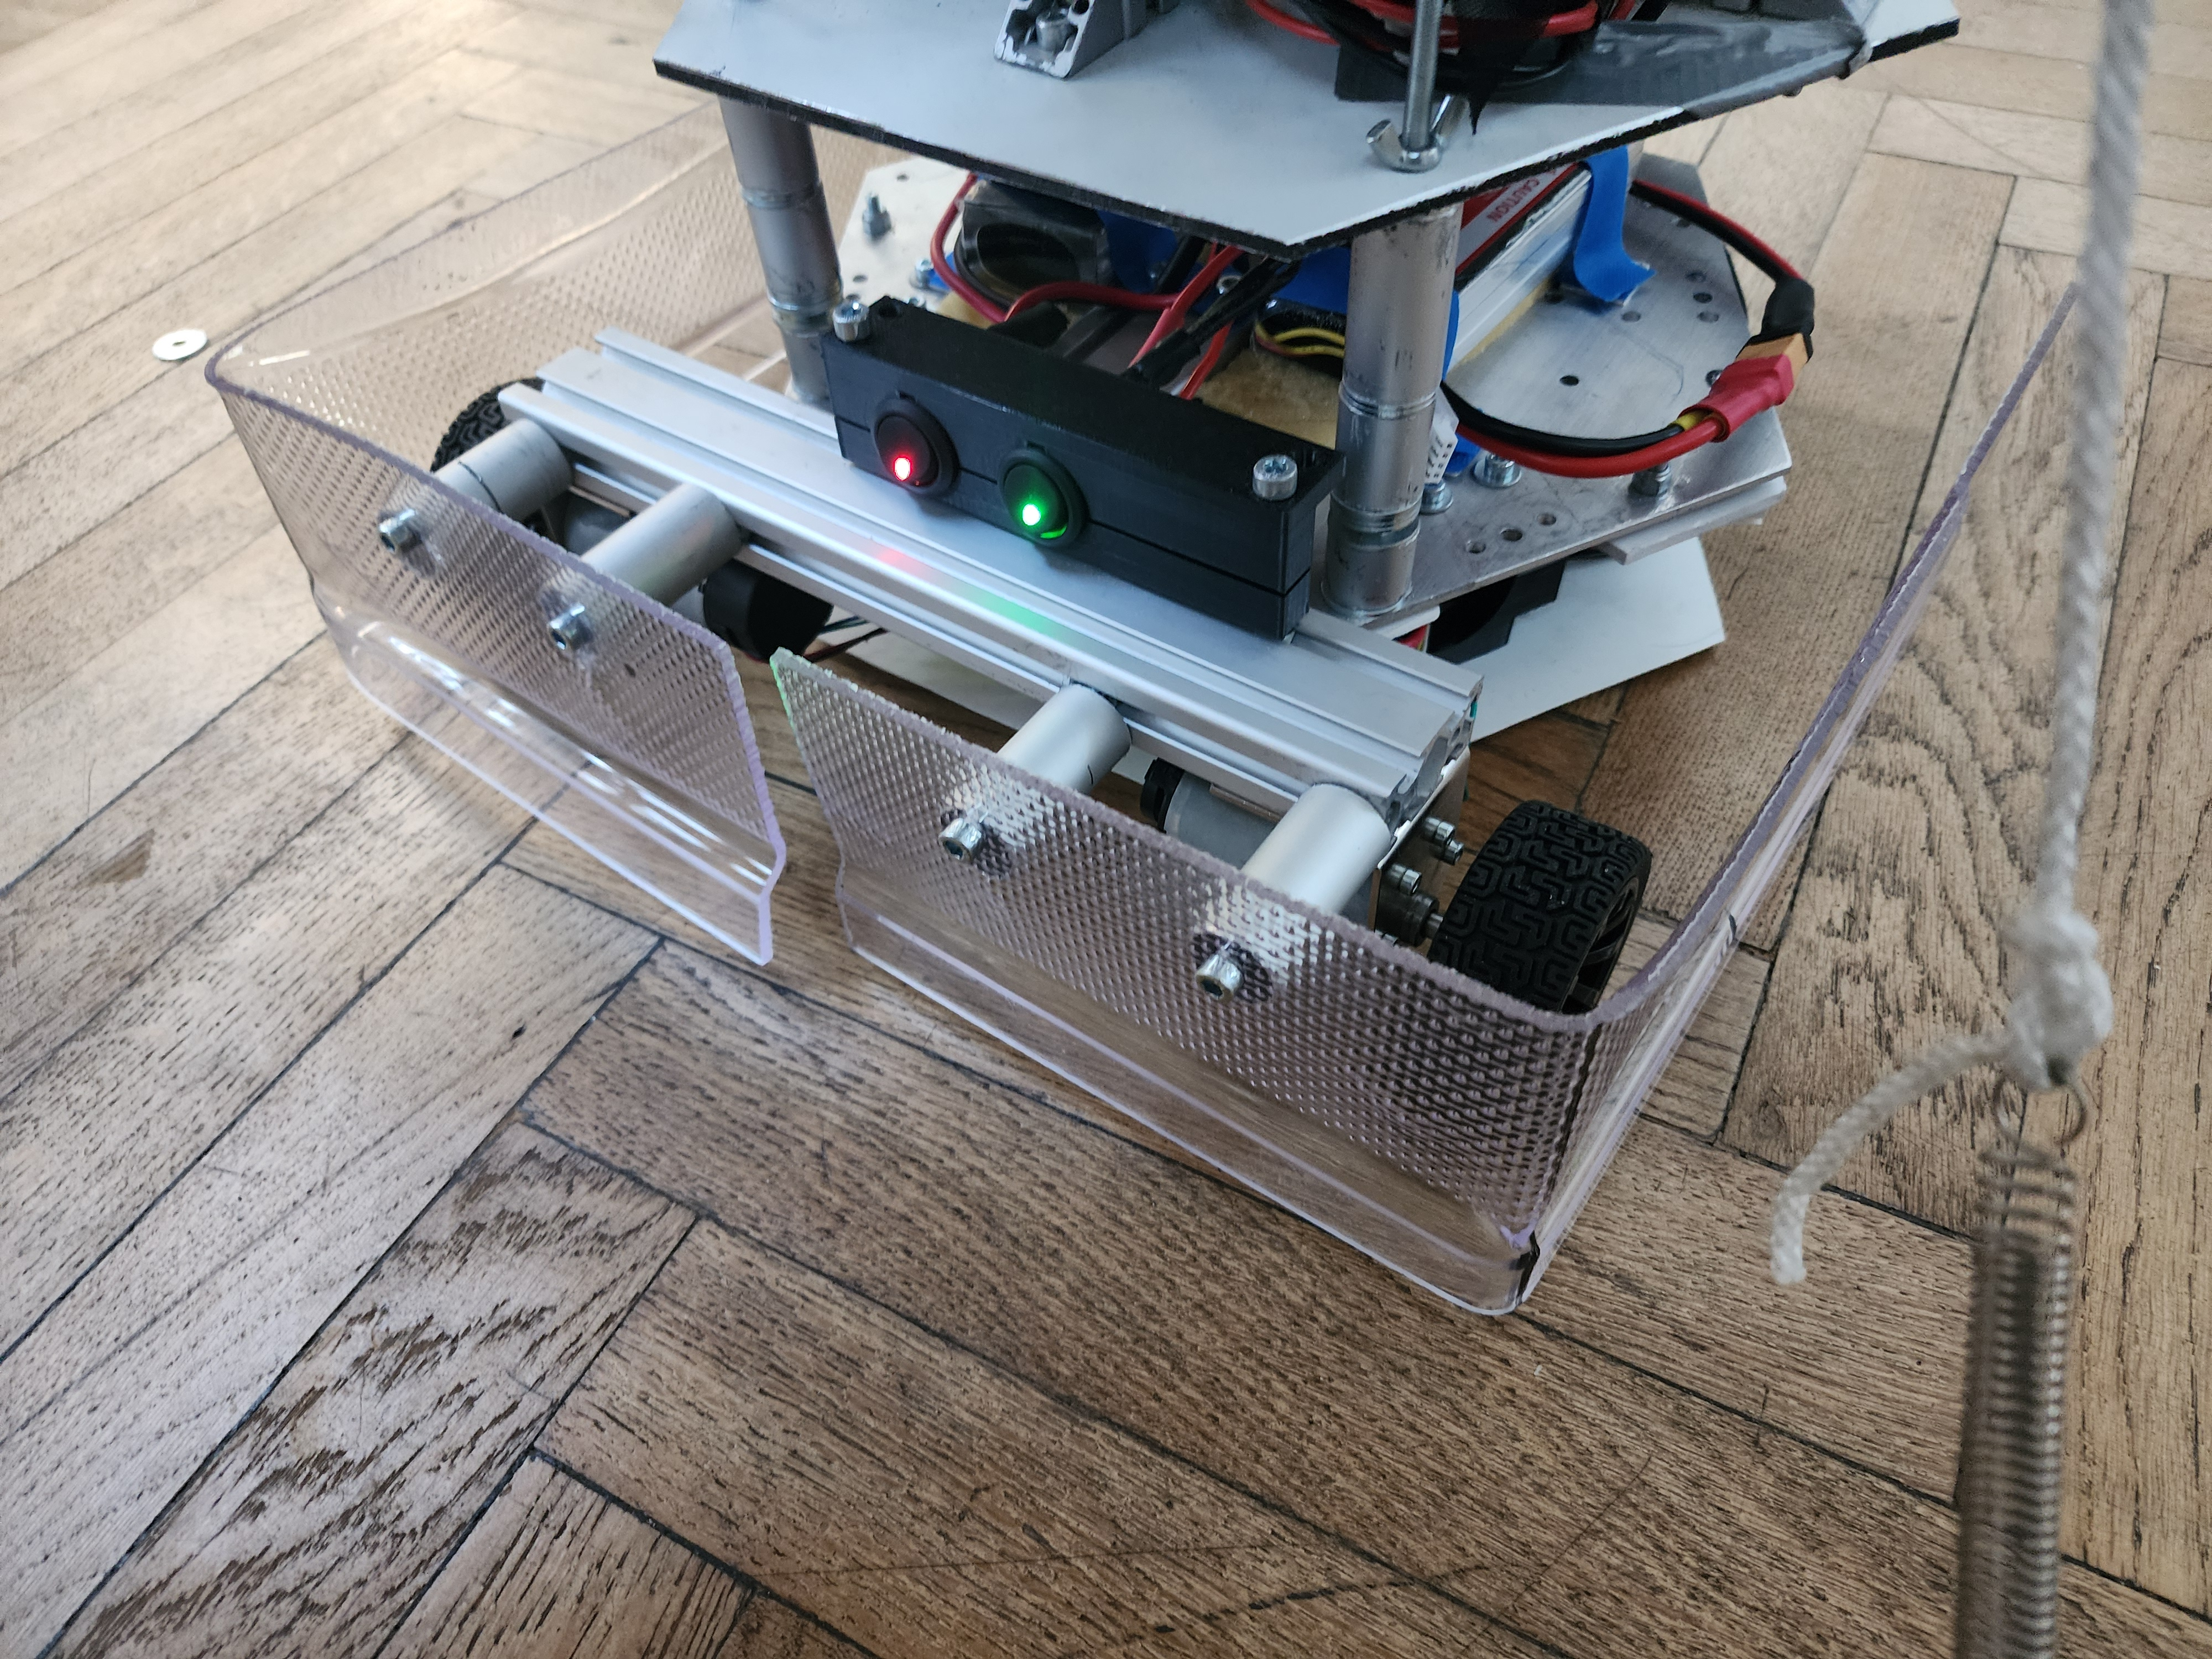
\includegraphics[width=\textwidth]{Images/TinoBumper (4).jpg}
        \caption{Tino Bumper Front View}
        \label{fig:tino_bumper_front}
    \end{minipage}
    \hfill
    \begin{minipage}{0.45\textwidth}
        \centering
        \includegraphics[width=\textwidth]{Images/TinoBumper (5).jpg}
        \caption{Tino Bumper Top View}
        \label{fig:tino_bumper_top}
    \end{minipage}
\end{figure}

The control system adaptation required comprehensive modification to support differential drive kinematics while maintaining compatibility with existing command interfaces. A custom PID controller was developed specifically for differential drive characteristics, replacing the VirHas library with optimized algorithms utilizing Kp=7.3, Ki=5.6, and Kd=0.2 parameters tuned for MDD10A motor drivers. Motor speed calculation employs encoder feedback with 1920 pulses per revolution (PPR) encoders, while atomic movement control integrates four distinct movement states that support synchronized leg-base coordination for VR integration.

\begin{figure}[H]
    \centering    \includegraphics[width=0.8\textwidth, angle=-90]{Images/TinoOnNewBase.jpg}
    \caption{Tino's new Base}
    \label{fig:tino_on_new_base}
\end{figure}

Motor speed calculation employs encoder feedback with 1920 pulses per revolution (PPR) encoders through the \texttt{getMotorSpeed()} function, enabling closed-loop speed control for precise movement execution. The \texttt{updatePid()} function implements the complete PID algorithm with integral term reset, derivative damping, and output limiting to ±255 PWM range, ensuring stable motor control without oscillation.

The \texttt{updateBaseMovementByTime()} function manages four distinct movement states that implement atomic operation completion where each movement phase must finish before accepting new commands. This prevents interrupted motions that could compromise synchronized robot behavior during VR integration. With the kinematic base providing reliable mobility, the system required enhanced power delivery capabilities to support the computational demands of the upgraded processing platform.

\subsection{Power Supply System}

The transition from Raspberry Pi to NVIDIA Orin Nano necessitated complete power system redesign to support significantly higher computational loads and multiple high-performance components. The legacy Raspberry Pi power distribution system proved inadequate for the Orin Nano's 19V DC requirement, Oak-D Pro camera power demands, and enhanced router system, requiring comprehensive architecture overhaul with consolidated battery management and efficient DC-DC conversion.

\subsubsection{System Requirements and Power Analysis}

The Orin Nano requires 19V DC input with power consumption reaching up to 2A during maximum computational load scenarios including simultaneous SLAM processing, human detection, audio processing, and ROS2 node operation. Typical operational consumption ranges between 1.3A to 1.4A during standard social interaction scenarios, with peak consumption of 38W during maximum load conditions and sustained operation typically requiring 25--27W. The power profile exhibits significant variation based on computational load, requiring robust power delivery capable of handling transient peaks without voltage drop.

Auxiliary system requirements include the Oak-D Pro camera system requiring 5V DC input with power consumption up to 5W during high-resolution stereo processing, and the onboard router system requiring 5V DC input with approximately 3W consumption during operational periods. Total system power budget analysis indicates maximum power consumption of approximately 46W under peak operational conditions, with typical sustained operation requiring 33--35W.

\subsubsection{Power Conversion and Distribution Implementation}

The power conversion system utilizes high-efficiency DC-DC converters to transform battery voltage to the multiple voltage levels required by system components. The Oumefar DC-DC step-up converter provides stable 19V output from 12V battery input with efficiency ratings exceeding 85\% across the operational load range, with converter selection prioritizing stability, efficiency, and thermal performance under sustained loading conditions. Power delivery stability testing demonstrated consistent voltage regulation within ±2\% across full load range with excellent transient response during computational load variations.

The 12V to 5V conversion system provides power for auxiliary components including the Oak-D Pro camera and onboard router, with power distribution architecture enabling independent power control for auxiliary components. 

\subsubsection{Battery System Consolidation and Performance}

The battery system redesign consolidates multiple power sources while providing enhanced capacity and reliability for extended operational periods. The primary battery system utilizes 5200mAh 80C 11.1V 57.72Wh LiPo batteries that provide the power density and discharge capabilities required for robotic applications, with battery specification analysis demonstrating adequate capacity for 2--3 hours of typical operation with conservative discharge management.

Maximum load operational time calculations indicate approximately 1.37 hours of operation under peak power conditions, though realistic operational scenarios typically achieve 2+ hours due to variable computational loading. The high discharge rate capability (80C) ensures stable power delivery during computational peaks without voltage sag, while the system consolidation reduces complexity from four separate battery systems to three integrated power sources.

The cable harness redesign eliminates obsolete USB-A and USB-C connections utilized for Raspberry Pi power delivery, replacing them with proper 12V distribution and 19V DC jack connectivity optimized for Orin Nano requirements. The 12V input distribution system provides primary power for both the step-up converter and the secondary 5V converter, with the 19V DC jack implementation providing secure power connection to the Orin Nano with proper mechanical support and electrical contact reliability.
% REORG_TAG: moved here from Stewart Platform Head Mechanism Improvements
\subsection{Stewart Platform Head Mechanism}

The Stewart platform head mechanism required iterative design improvements to address systematic reliability issues encountered during extended operational periods. The original implementation exhibited servo axis misalignment that created excessive stress concentrations on servo motor internals during head movement operations, with force analysis revealing that head loads were transmitted directly through servo shafts rather than through the structural framework. Additionally, the connecting arms showed excessive structural flexibility that reduced head positioning precision and contributed to mechanical instability, with repeated arm failures occurring due to inadequate load distribution and material selection in the 3D printed PLA components.

\begin{figure}[H]
    \centering
    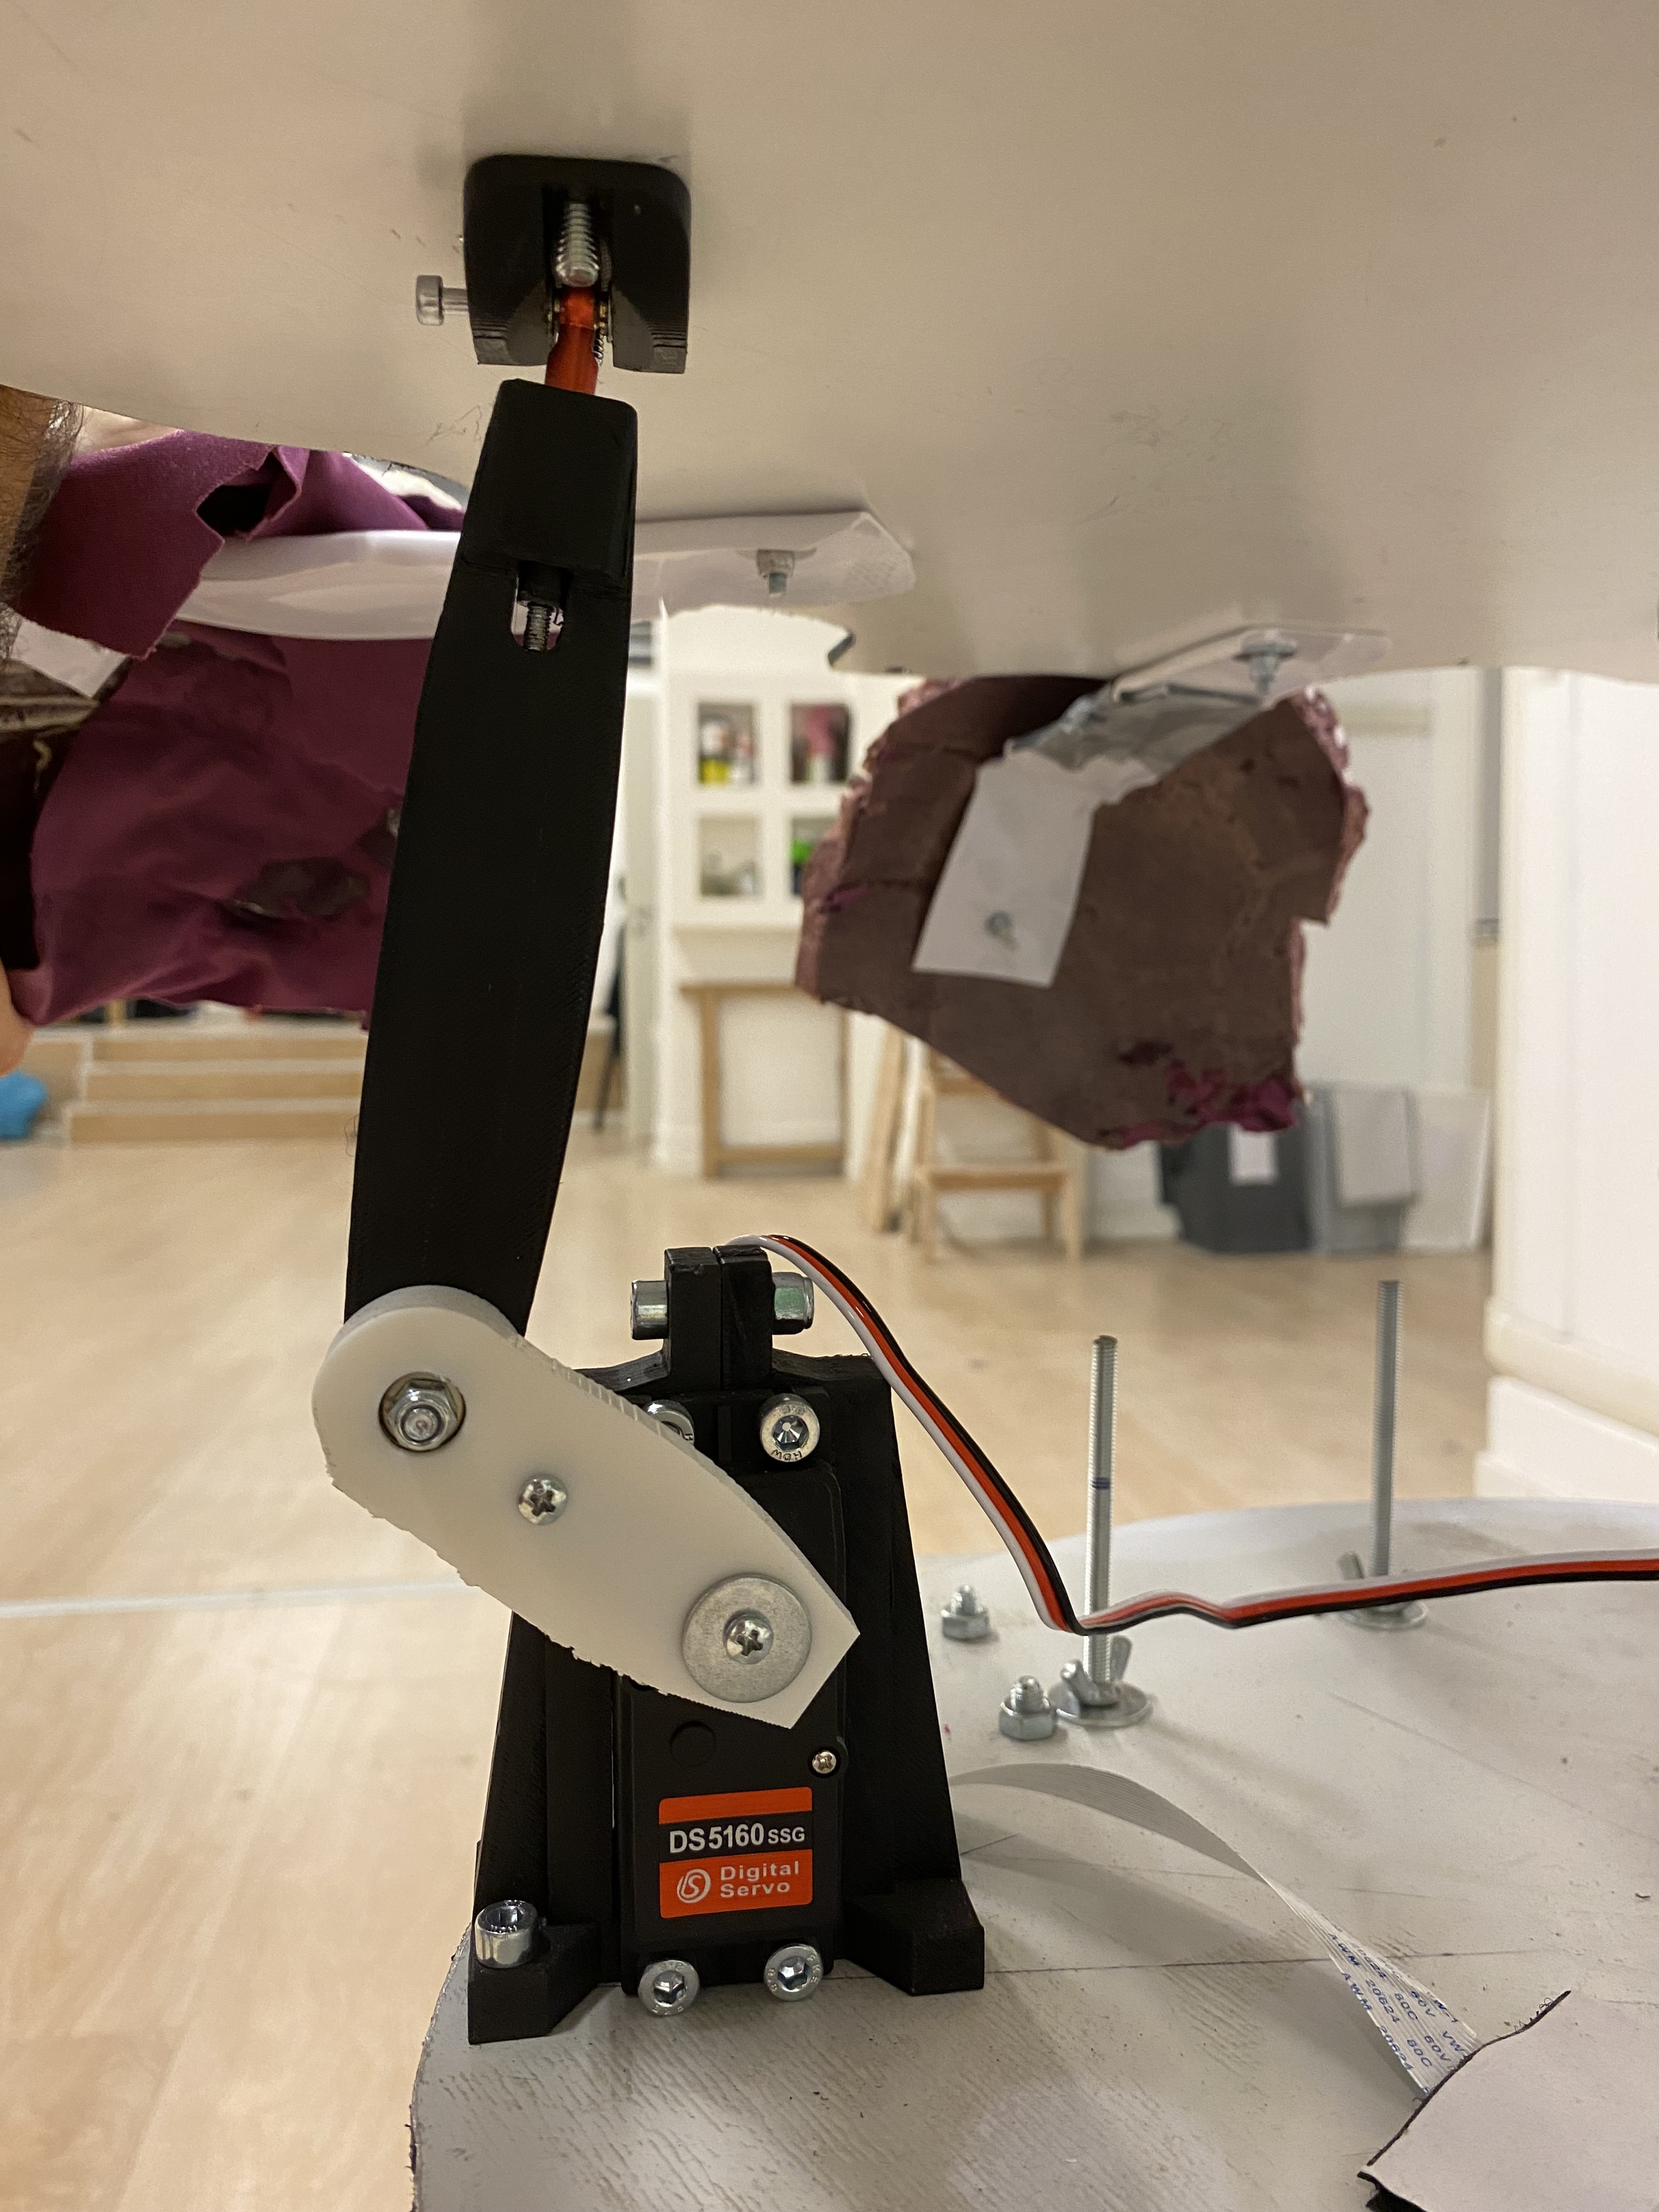
\includegraphics[height=6cm]{Images/signle_head_motor.jpg}
    \caption{Head Arm V0 Design}
    \label{fig:head_arm_v0}
\end{figure}

\subsubsection{Design Evolution and Failure Resolution}

The first design iteration focused on servo axis alignment to redirect forces through proper load paths while maintaining the existing bearing-based connection system. The servo axis alignment improvement redirected head loads through the structural framework rather than servo mechanisms, with enhanced PLA arm geometry providing improved load distribution through optimized cross-sectional design and stress concentration reduction.

\begin{figure}[H]
    \centering
    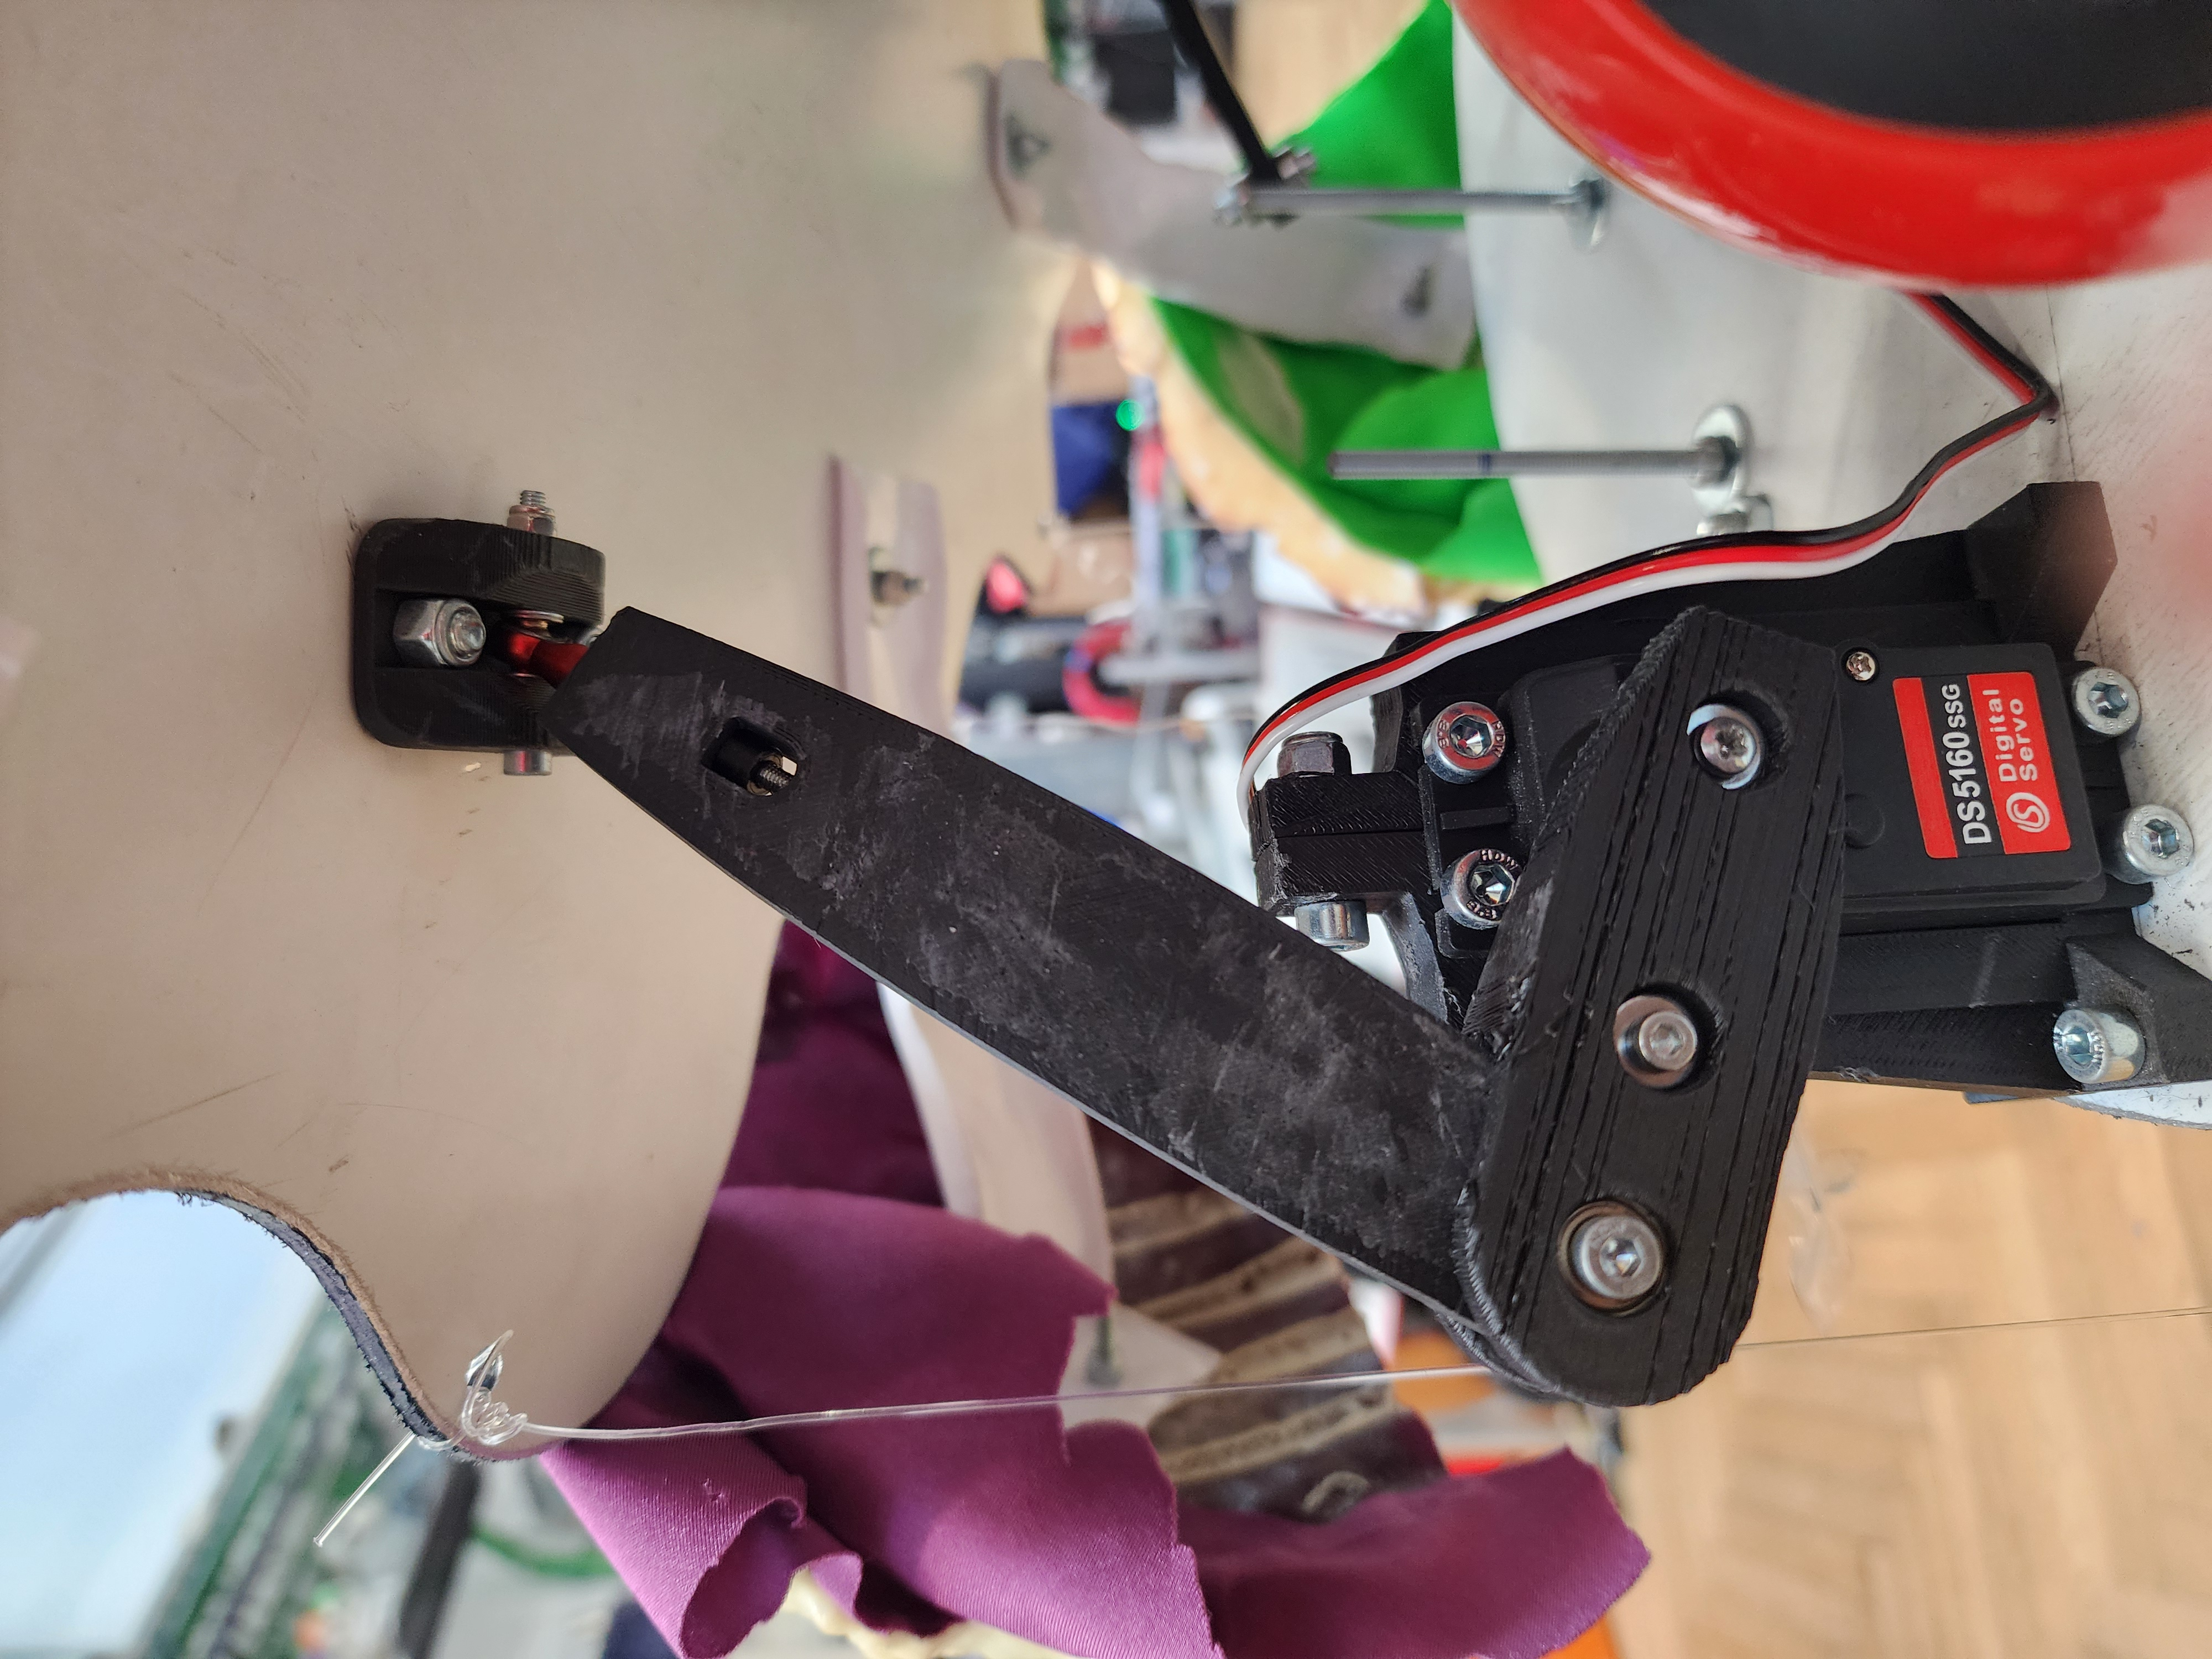
\includegraphics[height=6cm, angle=-90]{Images/HeadArmV2.jpg}
    \caption{Head Arm V1 Design}
    \label{fig:head_arm_v1}
\end{figure}

Performance evaluation demonstrated reduced servo stress indicators and improved movement precision, though structural flexibility issues remained due to the retained bearing connection system. Despite these improvements, the Stewart platform continued to experience significant structural flexibility problems that led to repeated arm failures during extended operational periods.

\begin{figure}[H]
    \centering
    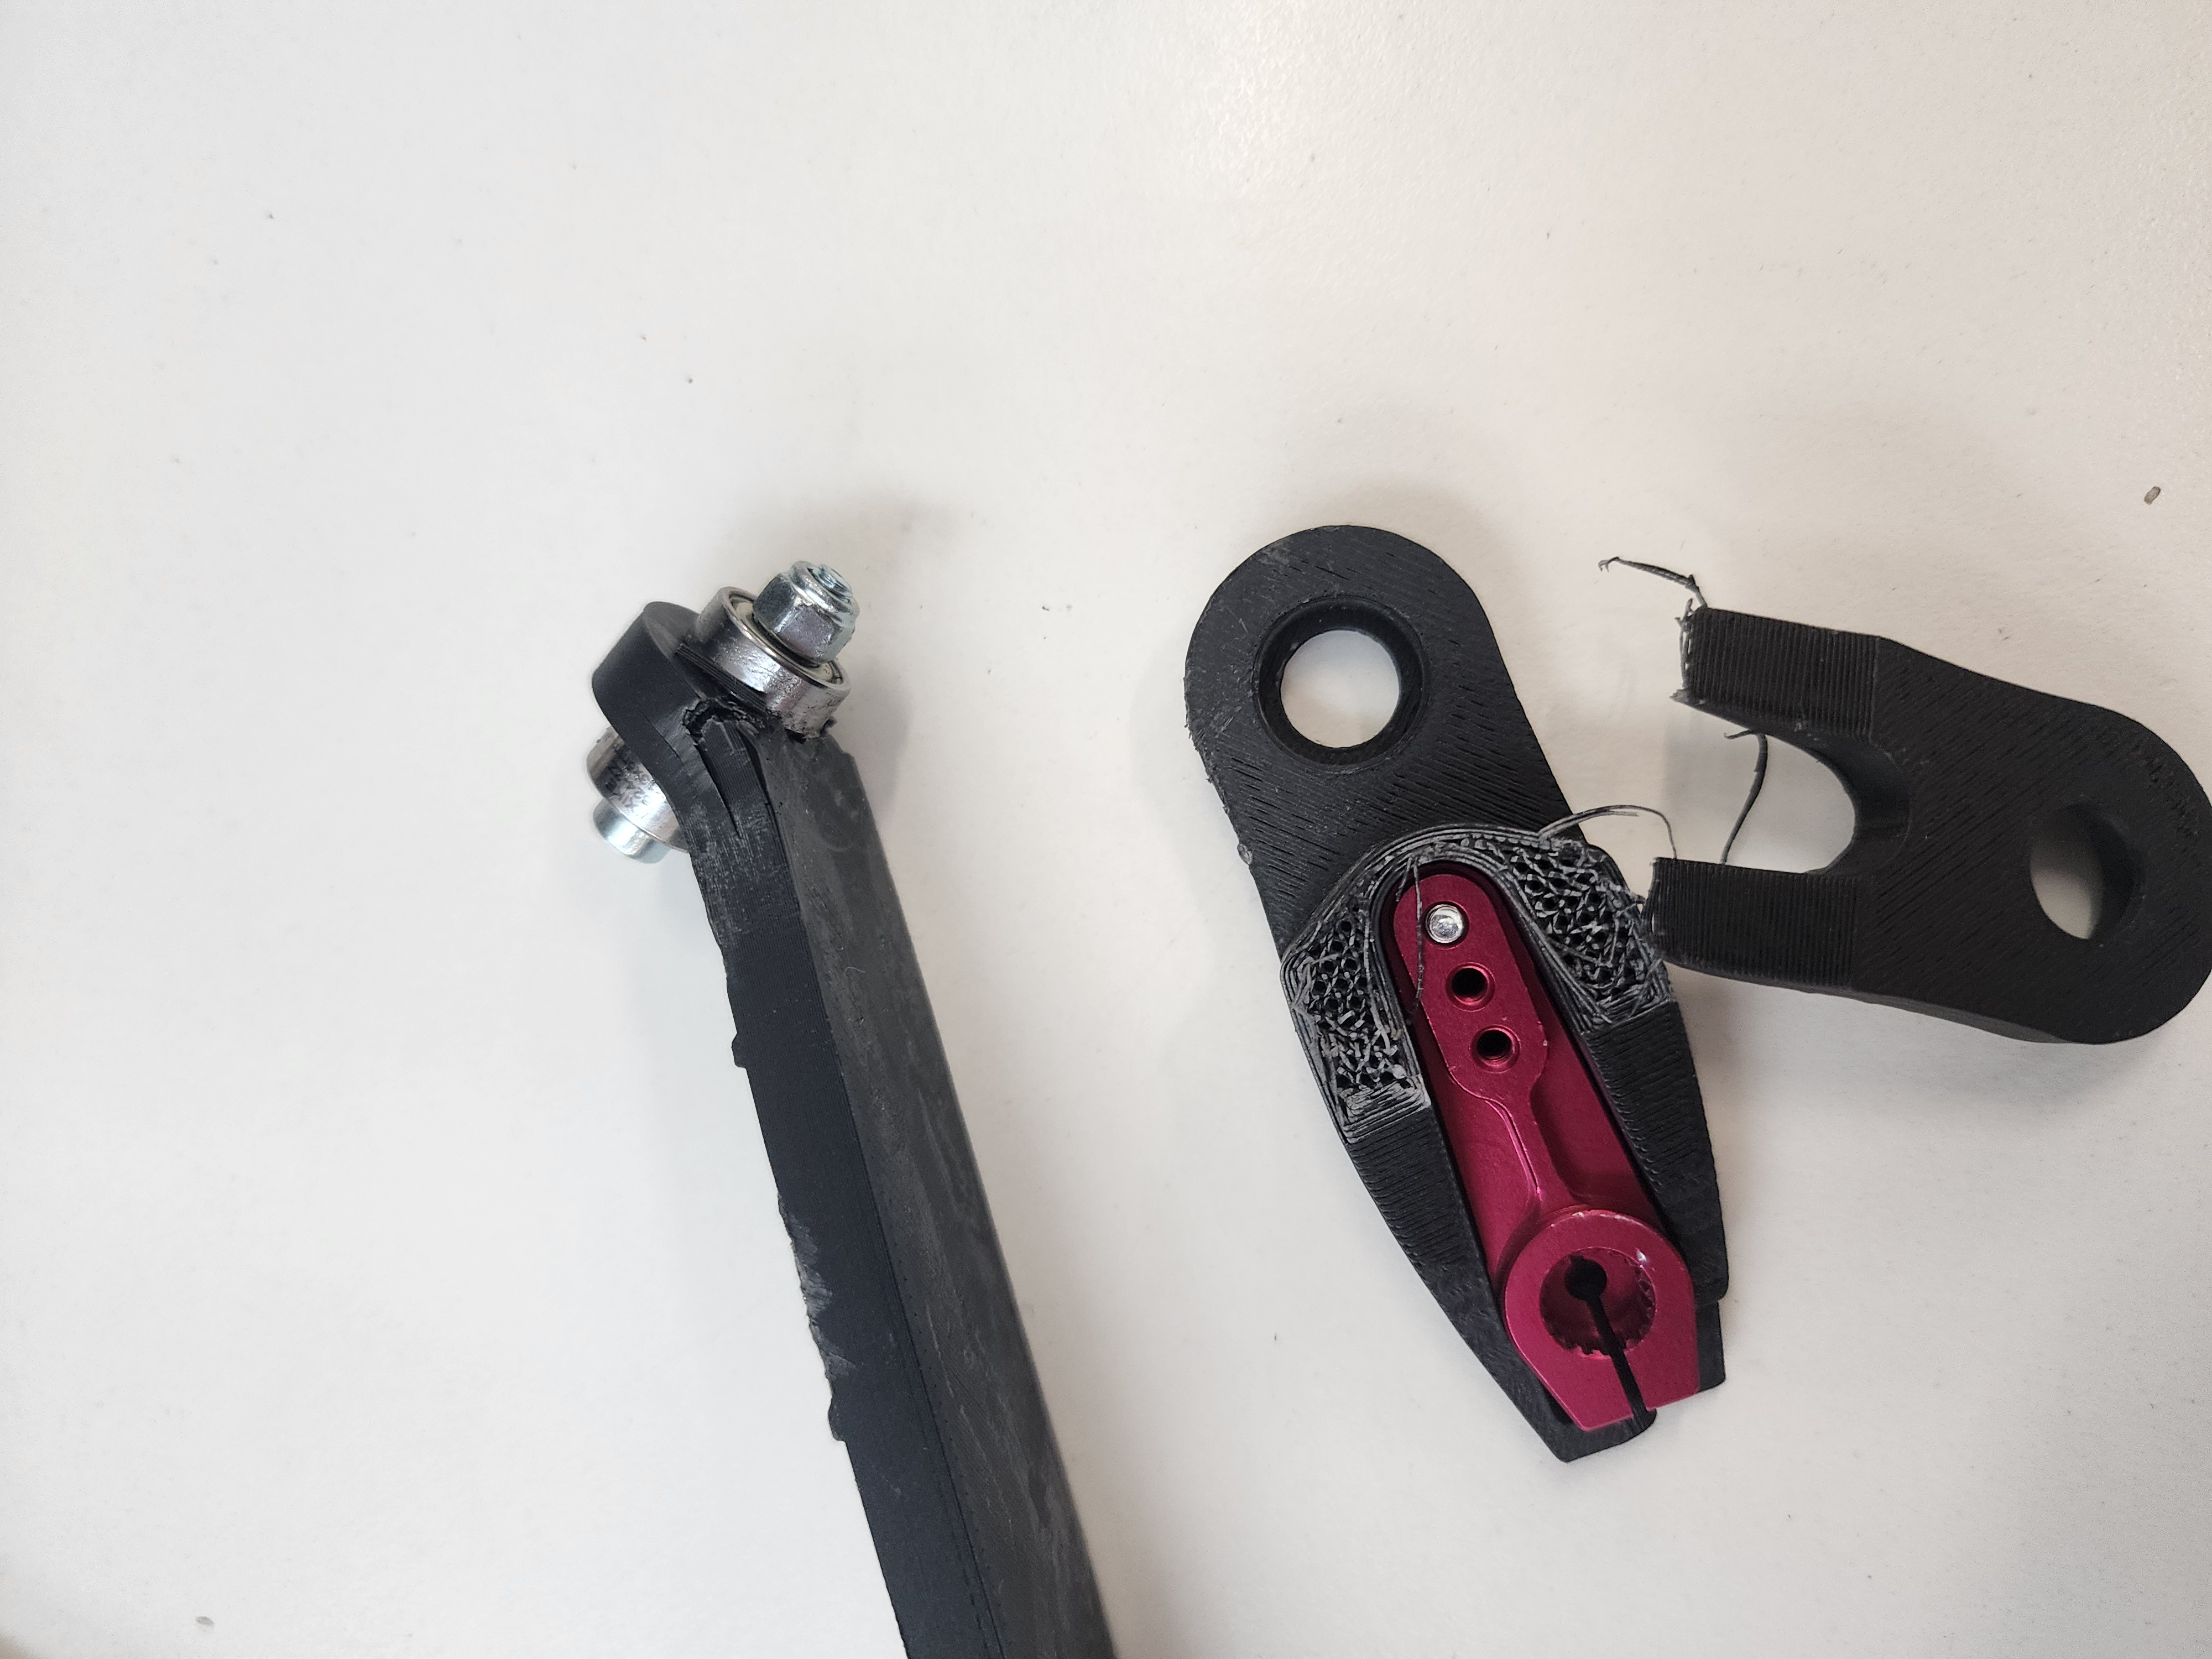
\includegraphics[height=6cm, angle=-90]{Images/HeadArmFailure (2).jpg}
    \caption{Head Arm Failure after Extended Use}
    \label{fig:head_arm_failure}
\end{figure}

The bearing connection system on the servo side of each arm introduced excessive compliance that compromised head positioning precision and contributed to continued mechanical instability. Failure analysis revealed that the 3D printed bearing housings could not adequately transfer forces between the improved servo connections and the head platform, with repeated stress cycling causing progressive degradation and eventual structural failure.

\begin{figure}[htbp]
    \centering
    \begin{minipage}{0.45\textwidth}
        \centering
        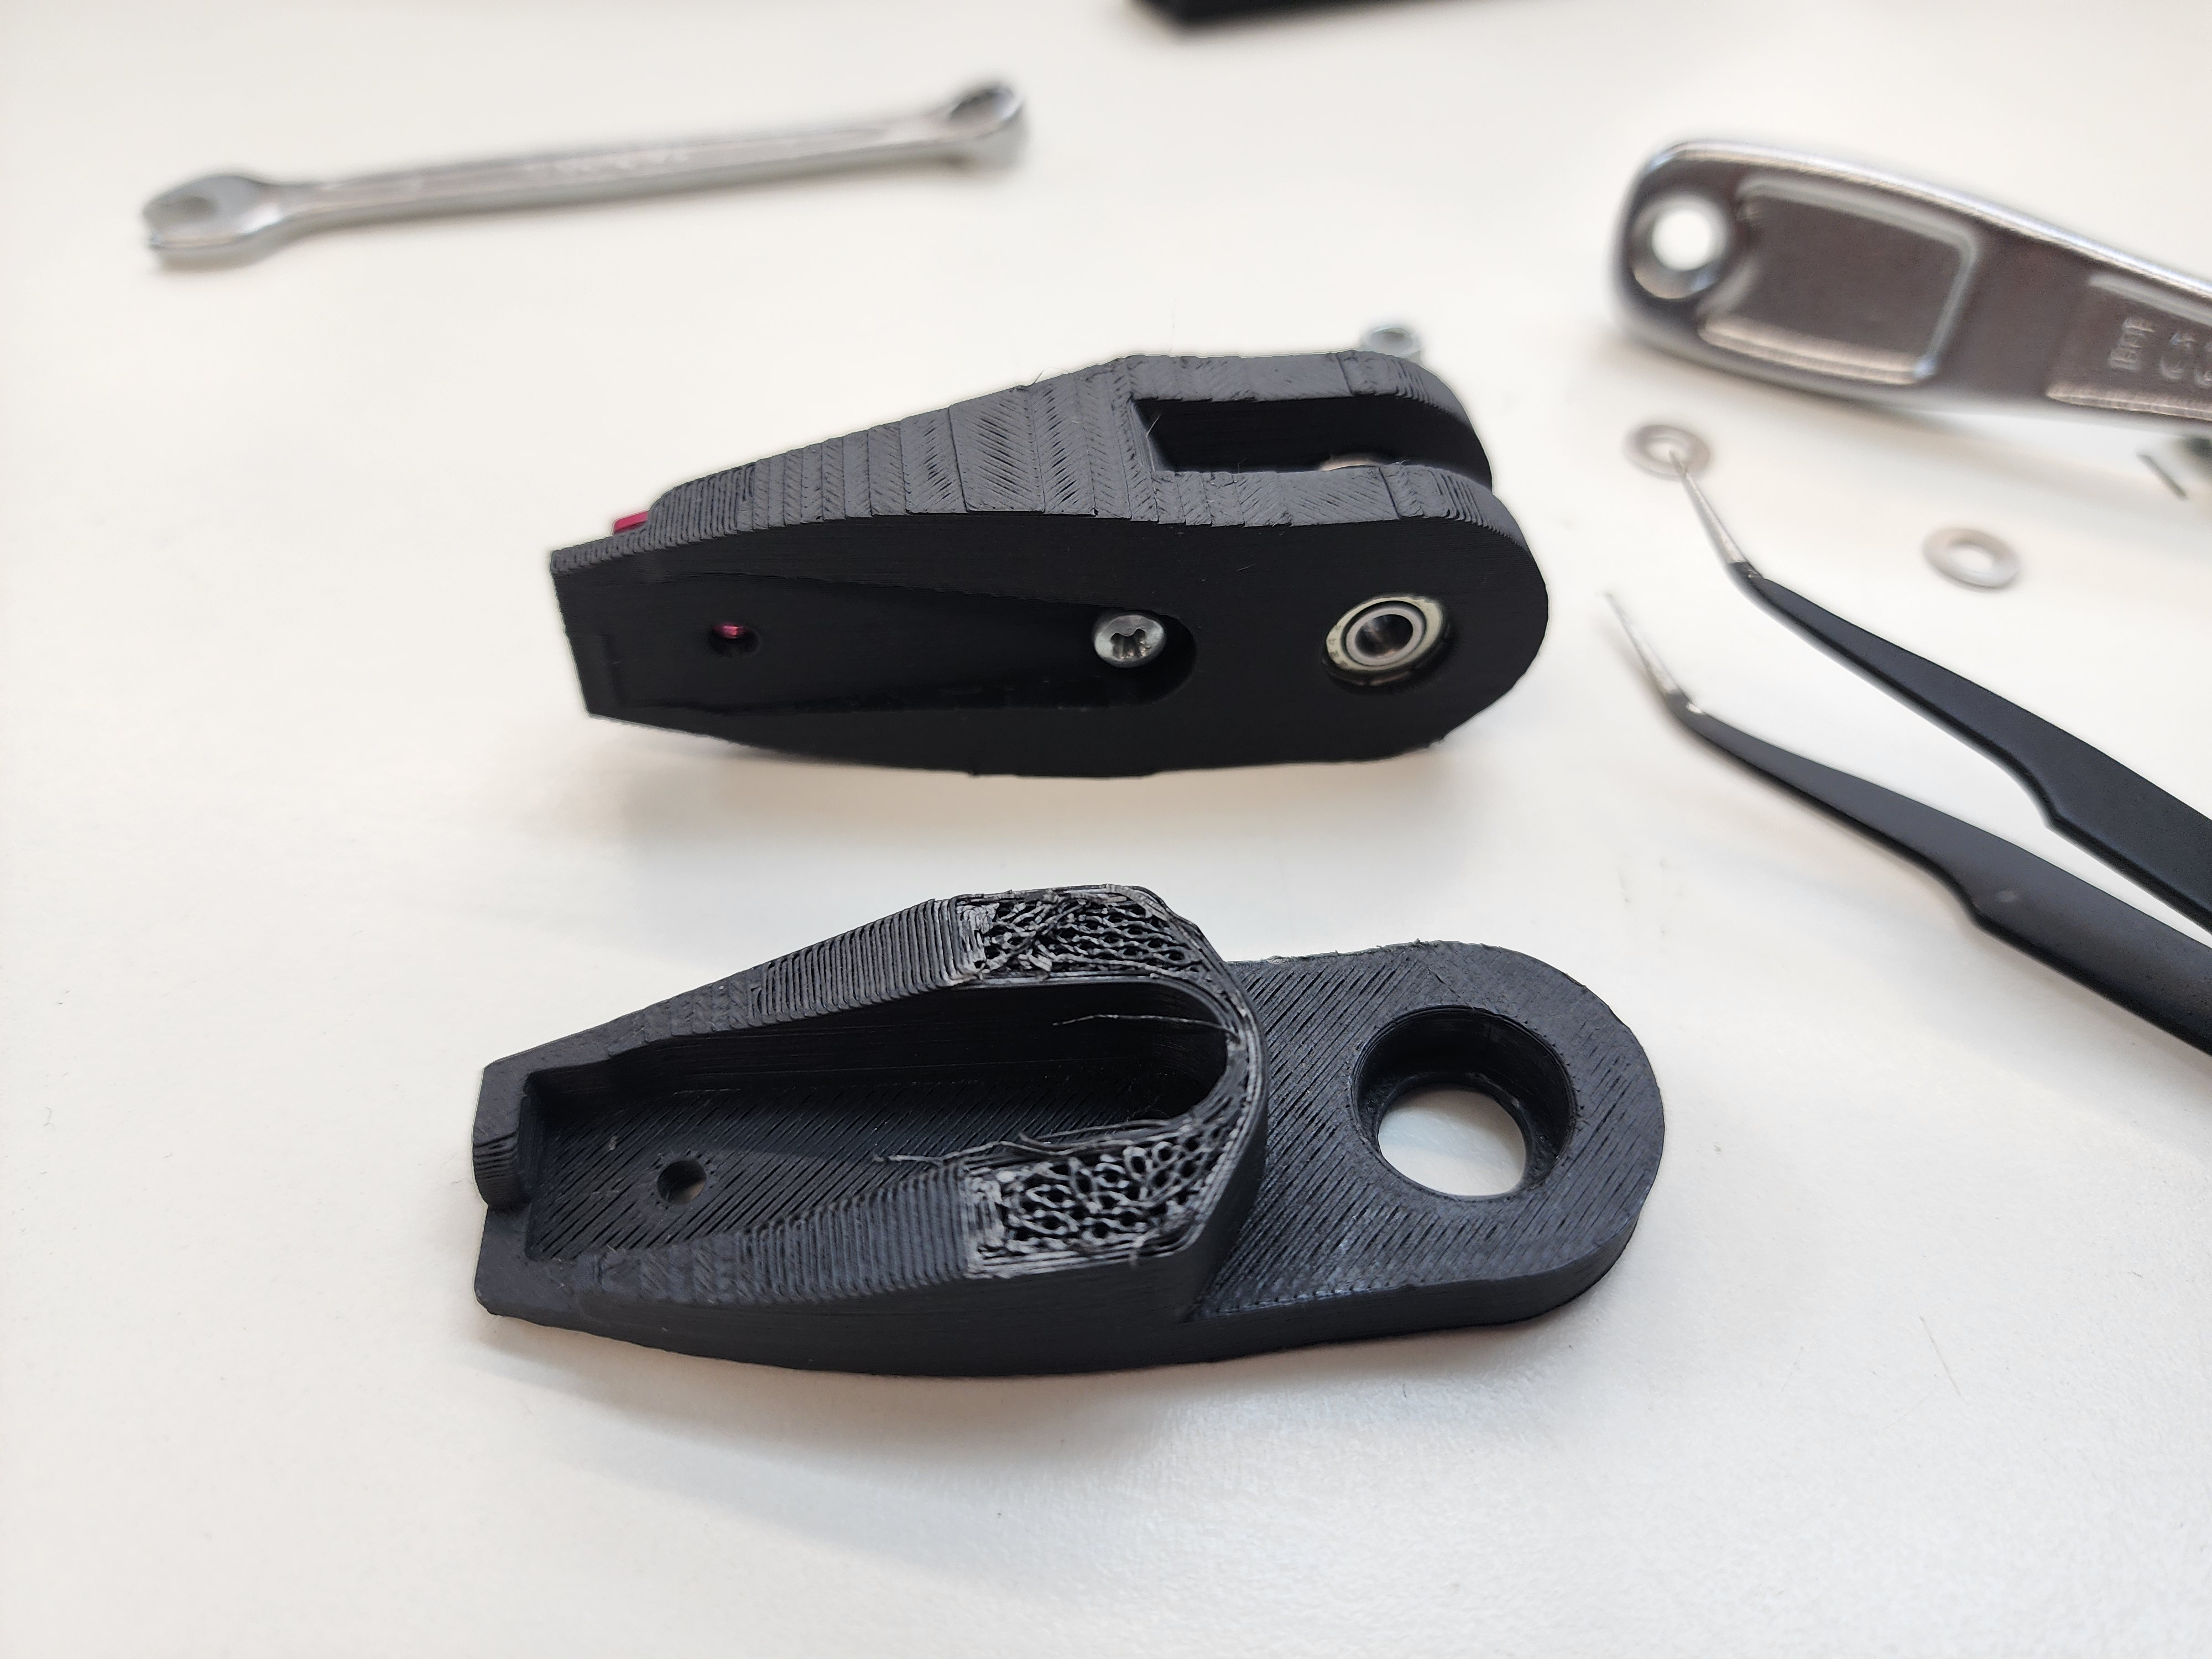
\includegraphics[width=\textwidth]{Images/HeadArmFailure (3).jpg}
        \caption{Servo Side Bearing Connection Failure}
        \label{fig:servo_bearing_failure}
    \end{minipage}
    \hfill
    \begin{minipage}{0.45\textwidth}
        \centering
        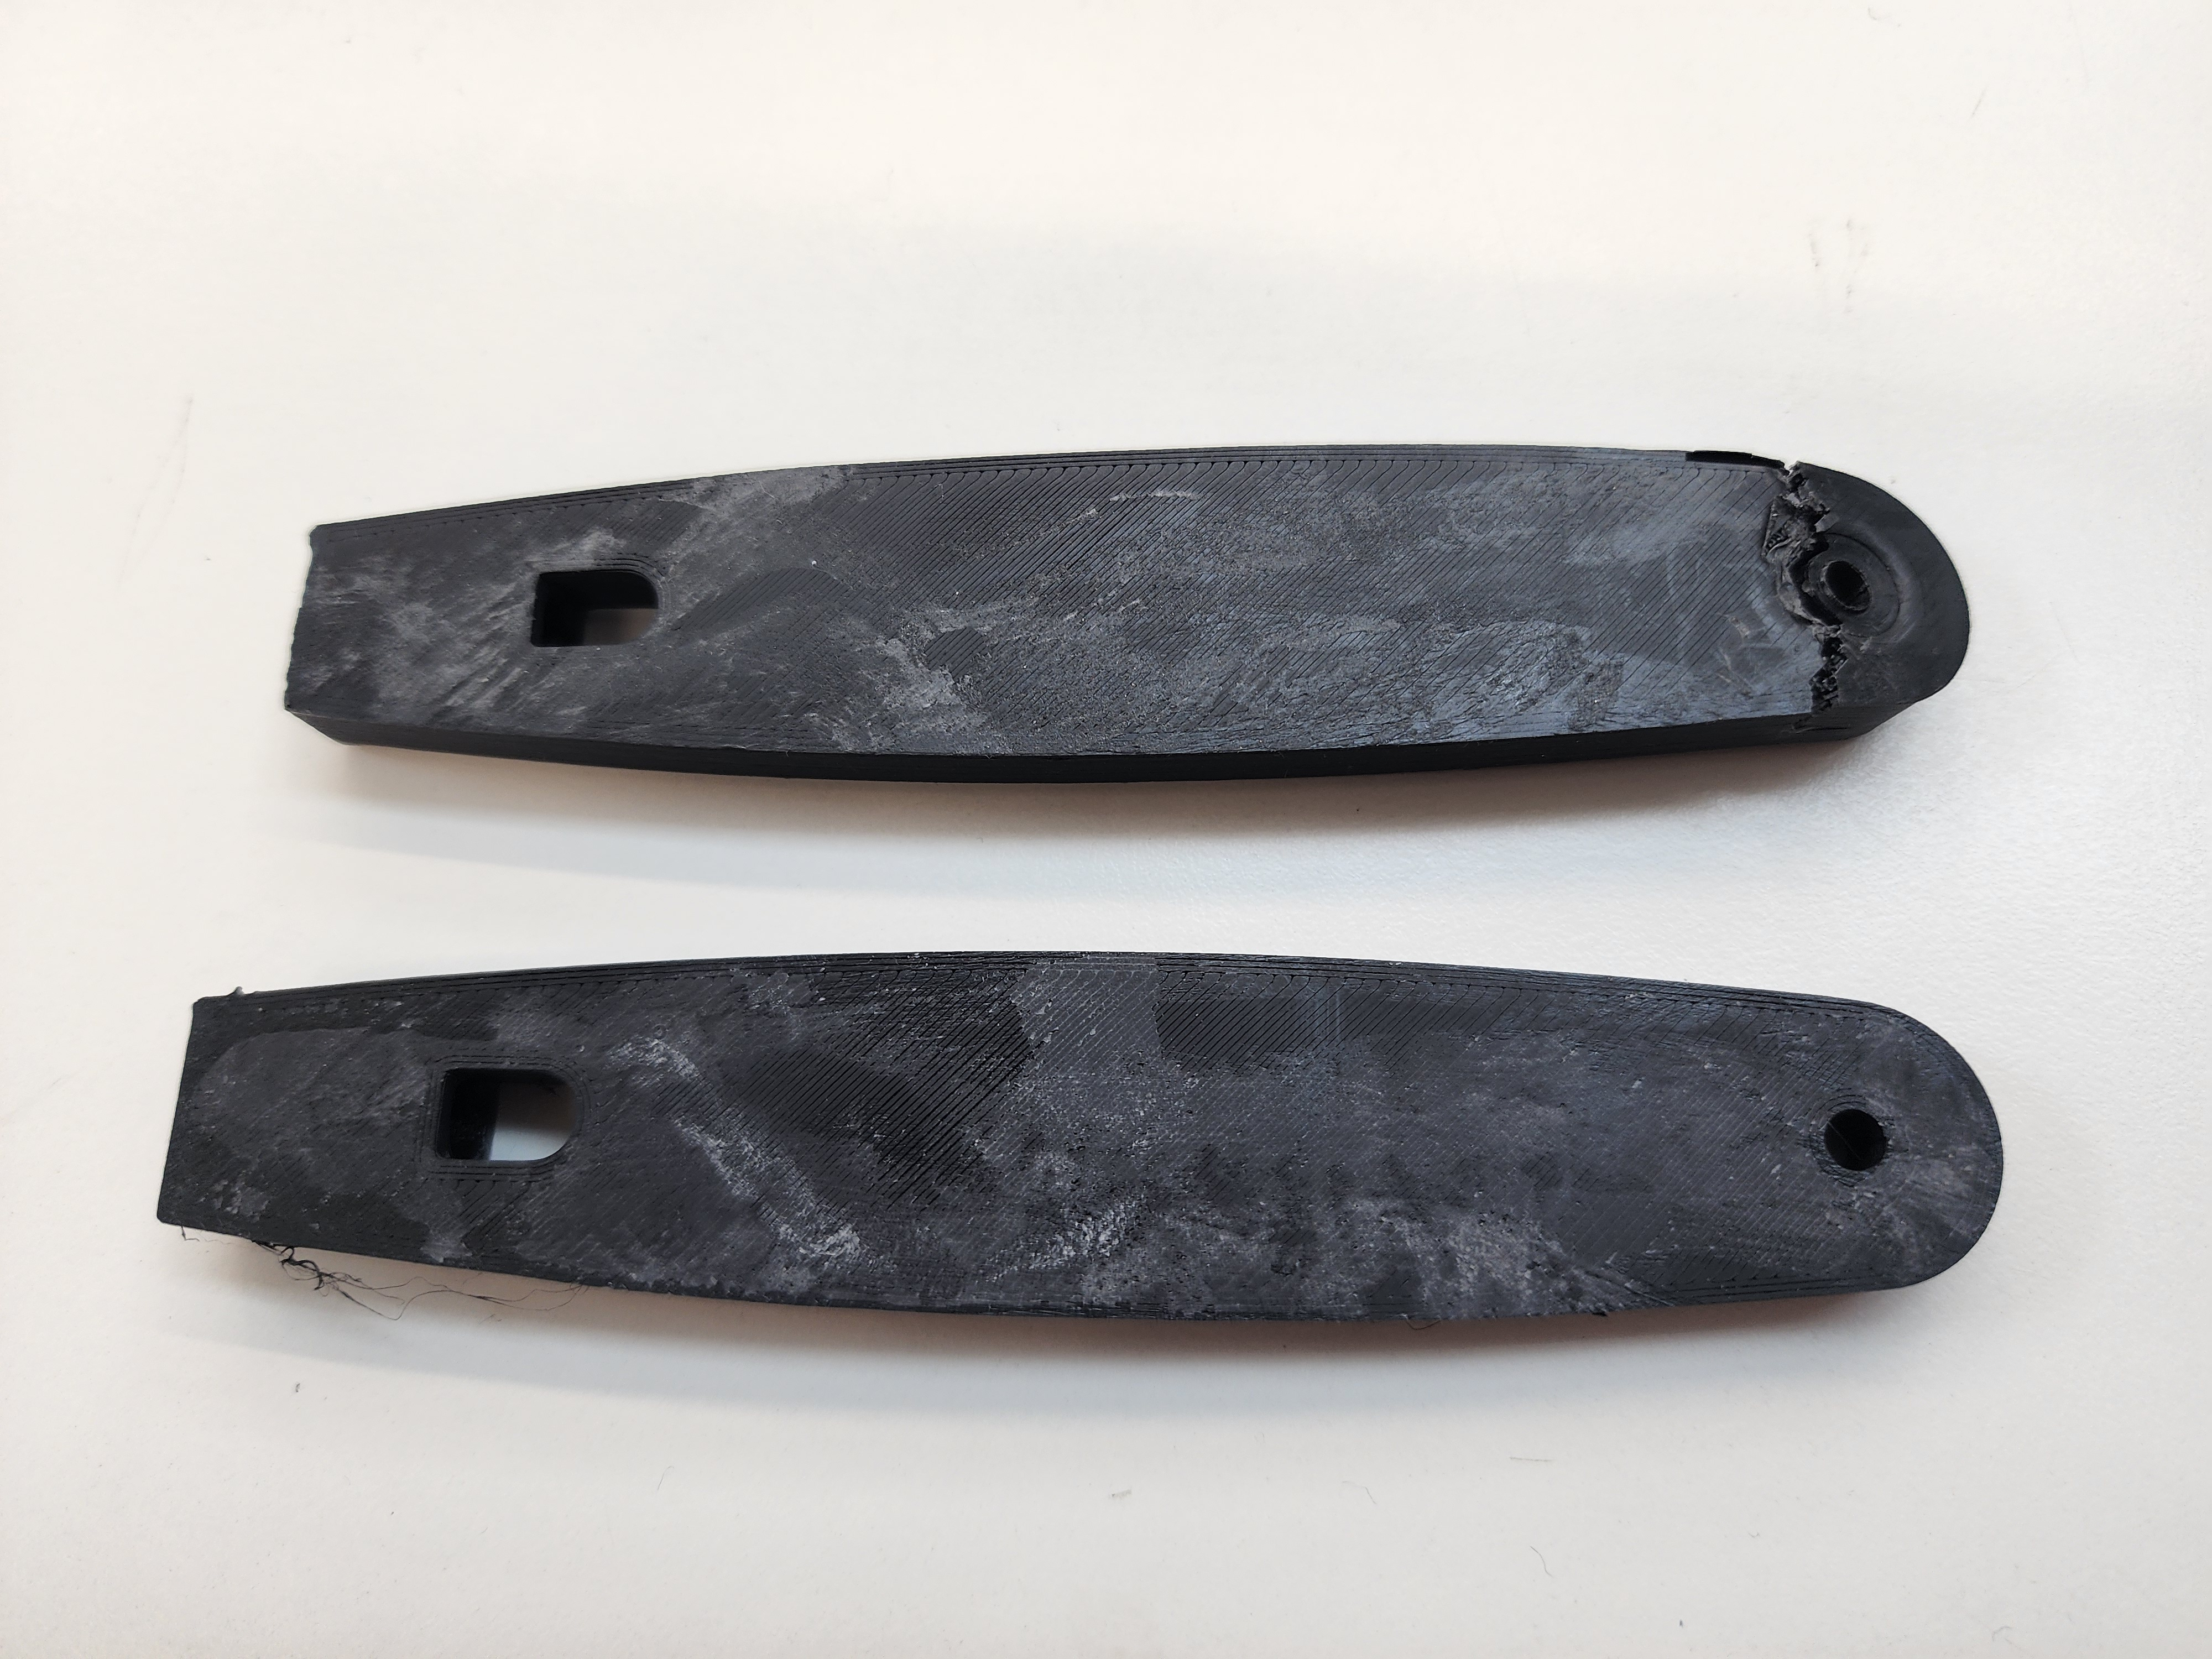
\includegraphics[width=\textwidth]{Images/HeadArmFailure.jpg}
        \caption{Head Arm Failure after Extended Use}
        \label{fig:head_arm_failure_alt}
    \end{minipage}
\end{figure}

\subsubsection{Rod End Solution Implementation}

The fundamental limitation resided in the conflict between smooth articulation requirements and structural rigidity within 3D printed PLA construction constraints. Research into Stewart platform best practices identified rod end connections as the standard solution for eliminating binding while allowing proper articulation throughout the movement range, leading to the final design iteration that adopted rod end (heim joint) connections on both ends of each Stewart platform arm.

\begin{figure}[H]
    \centering
    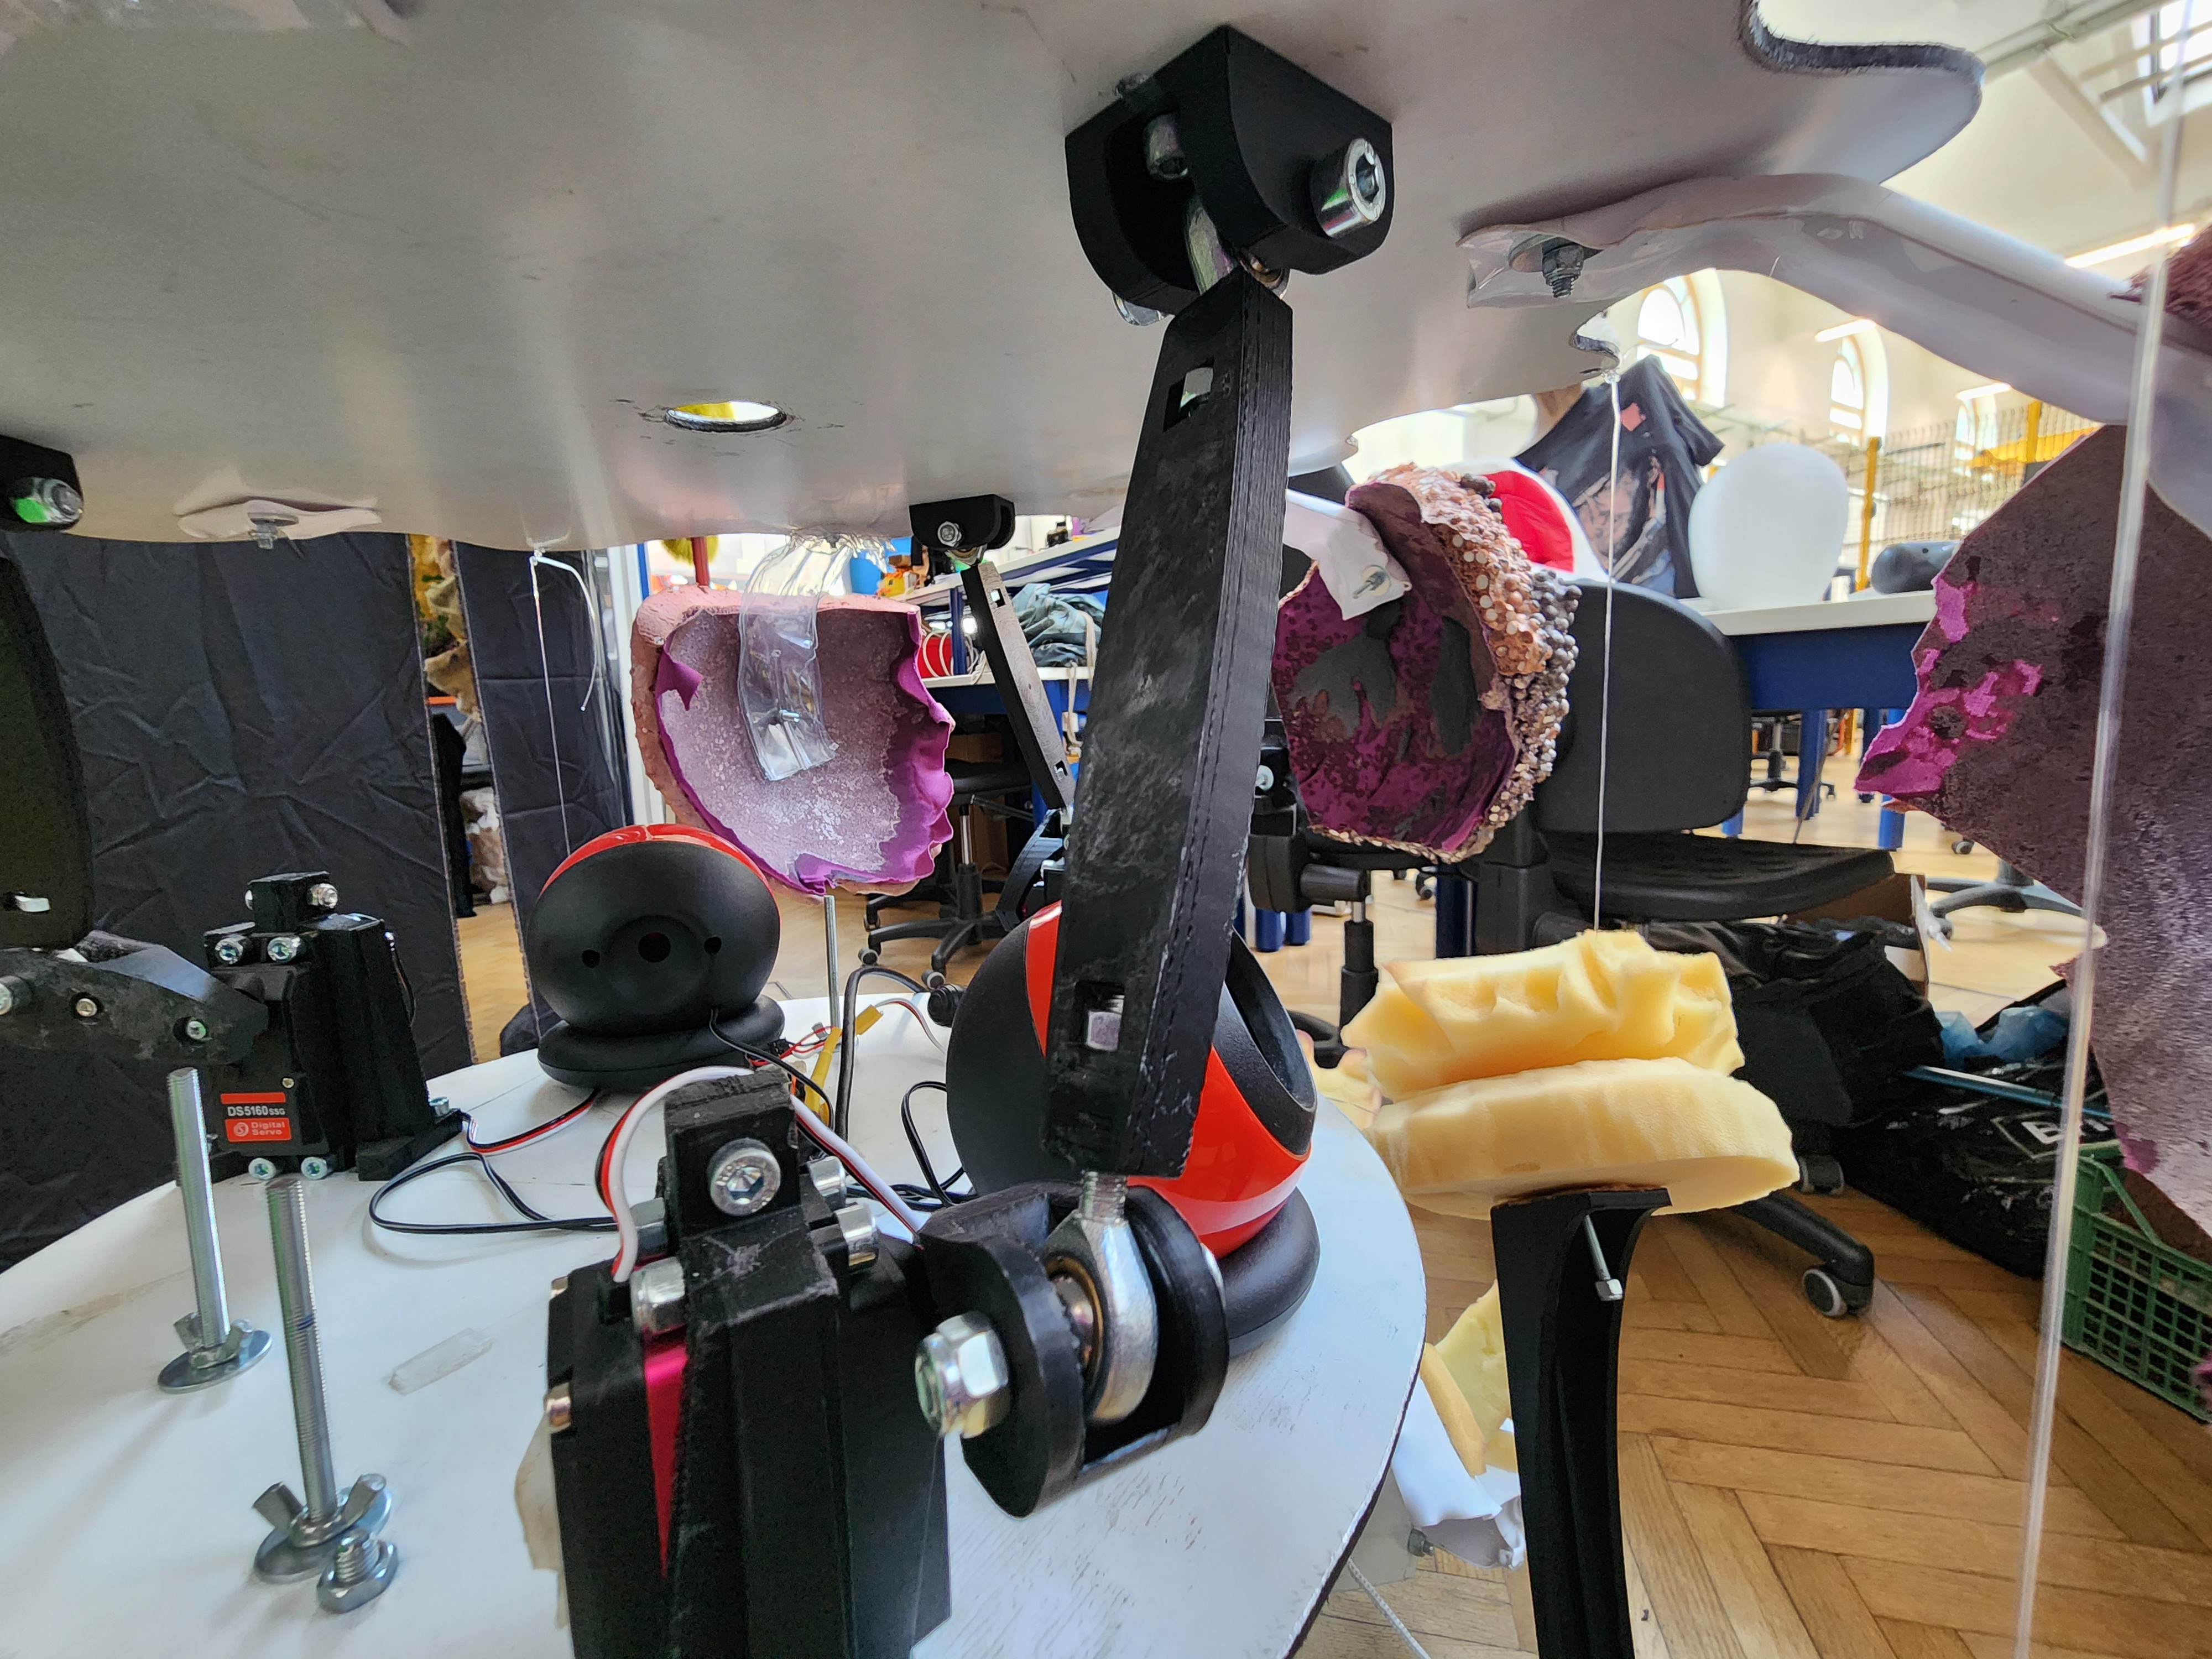
\includegraphics[height=6cm]{Images/NewHeadDoubleJoint (4).jpg}
    \caption{Head Arm V2 Design with Rod Ends}
    \label{fig:head_arm_v2}
\end{figure}

The rod end implementation utilizes metal heim joints that provide superior strength and durability compared to the original bearing system, with metal construction eliminating the brittleness and wear issues encountered with printed bearing housings. Joint articulation characteristics enable free rotation in all necessary axes while providing positive mechanical connection between arm segments, eliminating binding forces that contributed to servo stress and movement precision issues.

Mechanical trade-offs include acceptable head wobble during stationary periods due to free articulation provided by the heim joints, though analysis indicates this wobble may actually enhance Tino's expressive capabilities by providing natural movement characteristics. Structural strength analysis demonstrates significant improvement in mechanical robustness and load-bearing capability while accepting reduced precision during stationary periods.

\begin{figure}[H]
    \centering
    \begin{minipage}{0.45\textwidth}
        \centering
        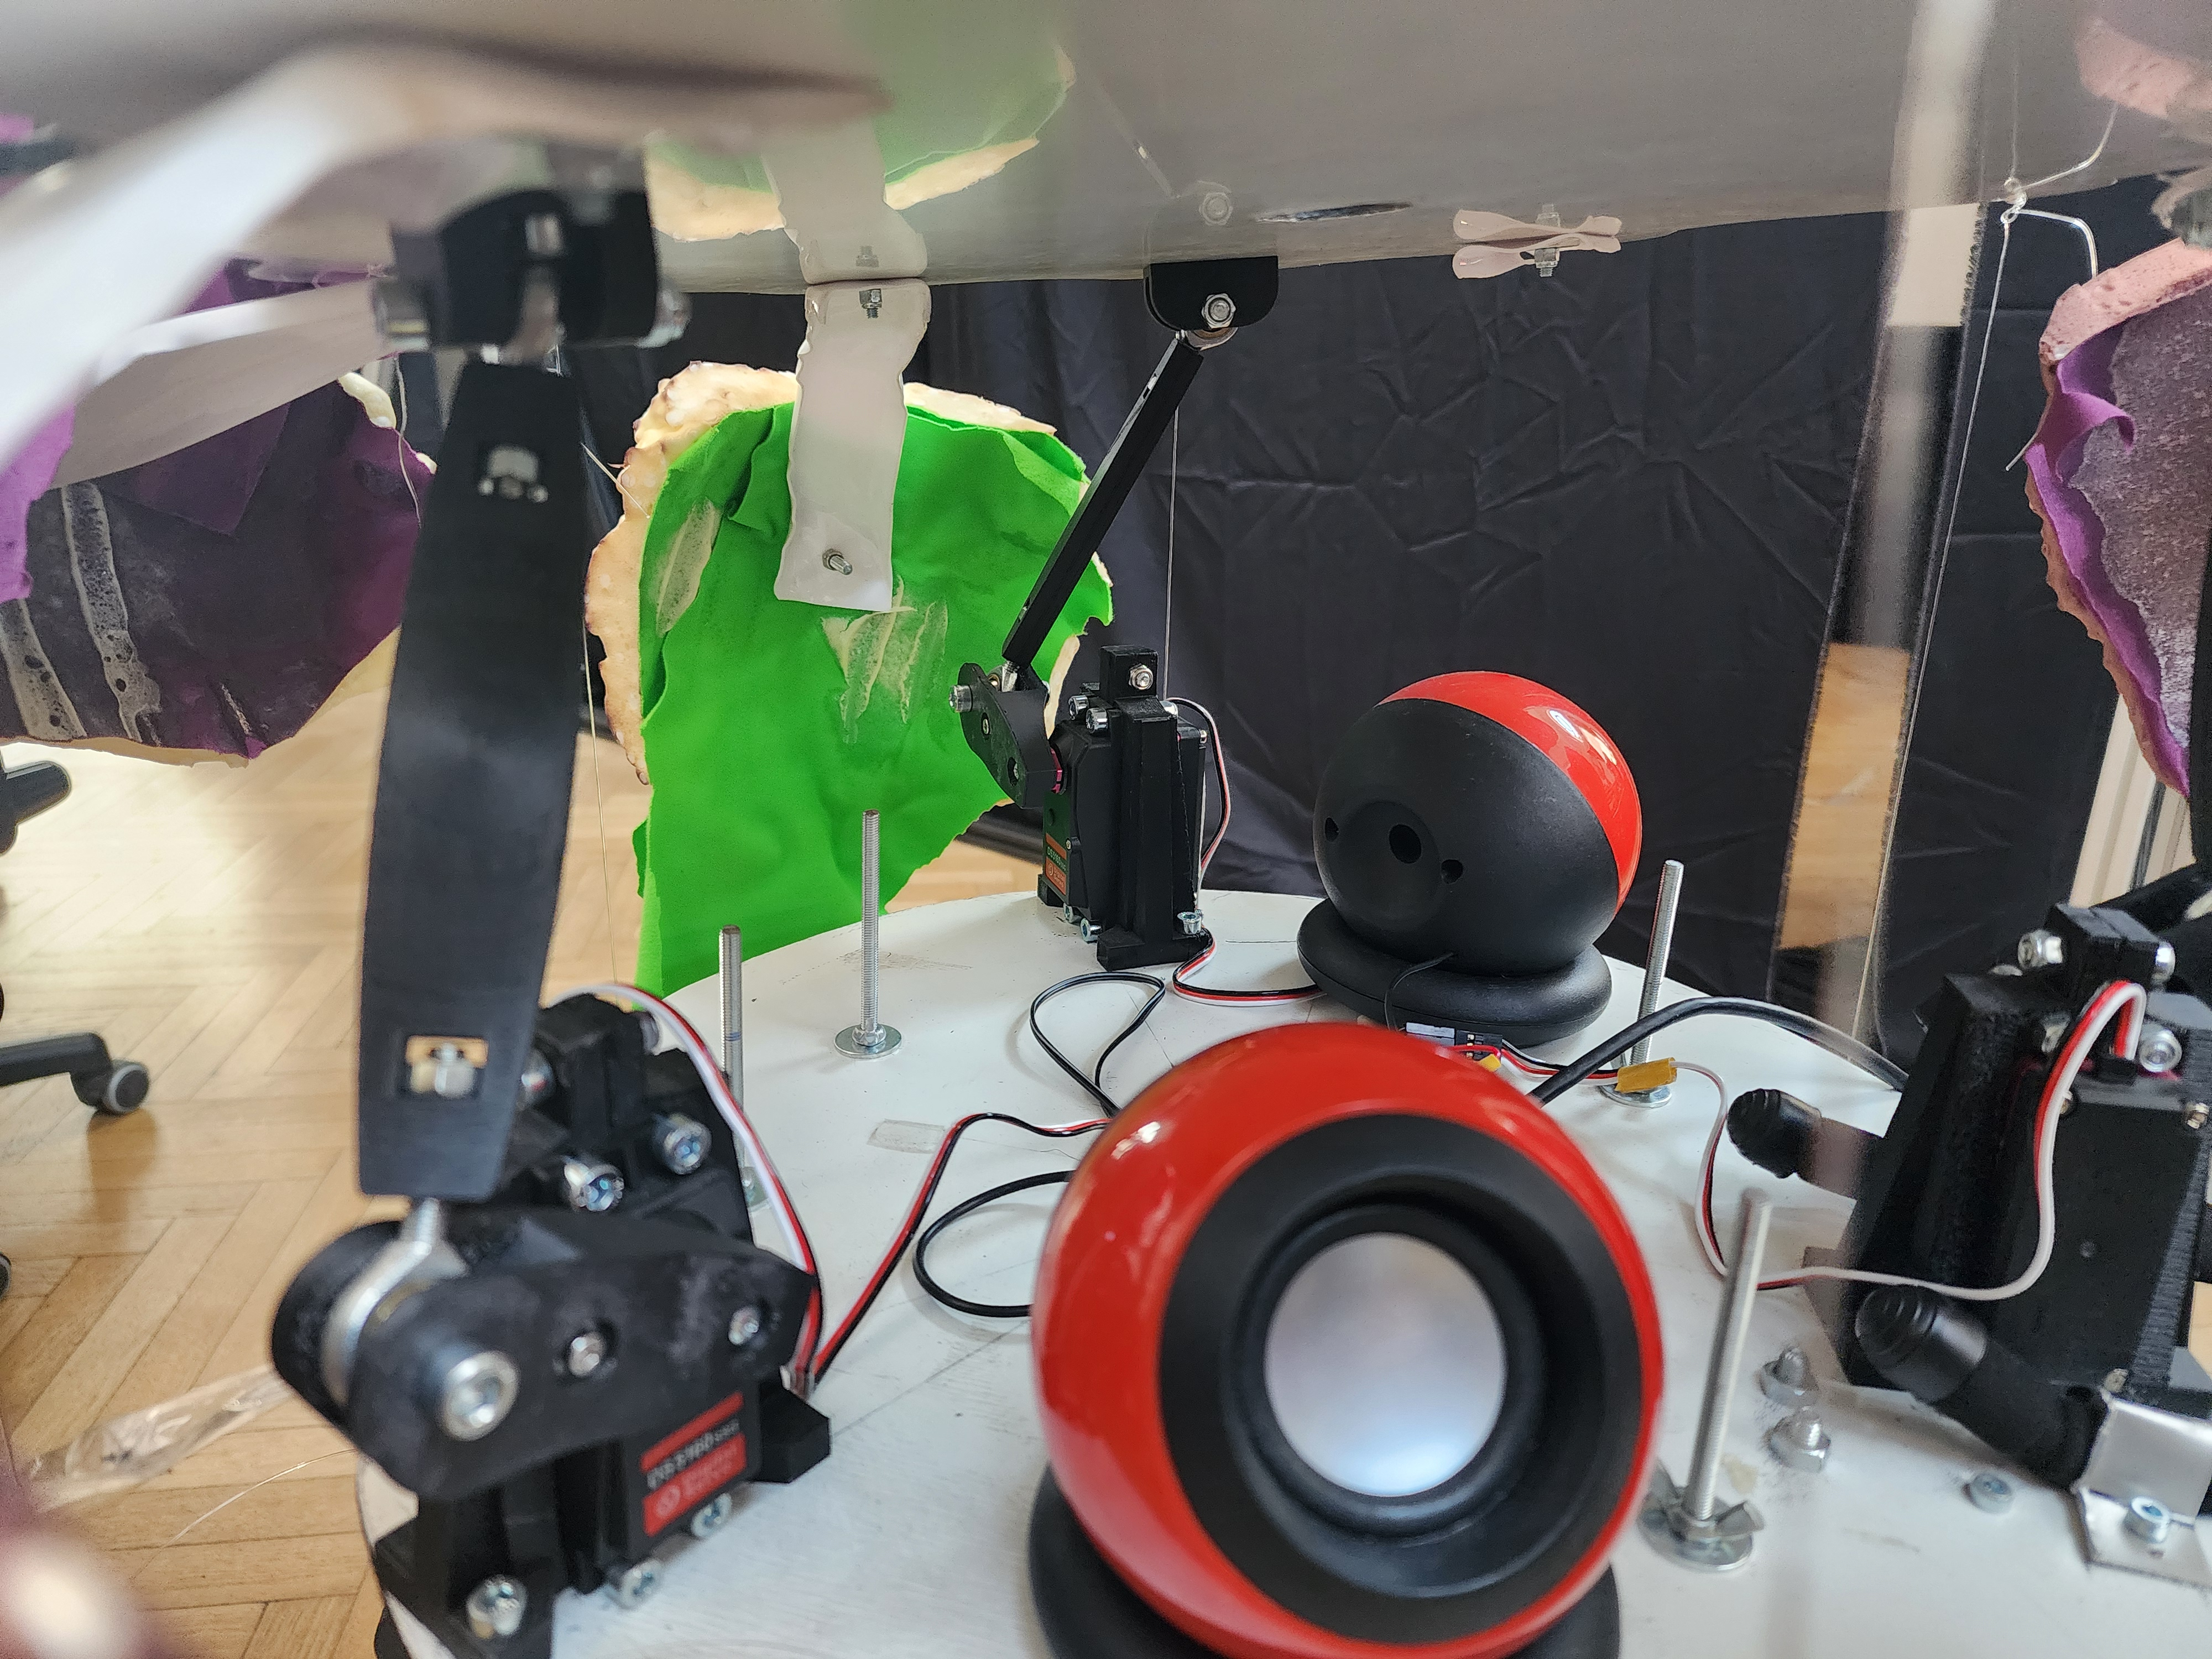
\includegraphics[width=\textwidth]{Images/NewHeadDoubleJoint (6).jpg}
        \caption{Head Arm with Rod Ends (Sway to right)}
        \label{fig:head_arm_rod_end_right}
    \end{minipage}
    \hfill
    \begin{minipage}{0.45\textwidth}
        \centering
        \includegraphics[width=\textwidth]{Images/NewHeadDoubleJoint (2).jpg}
        \caption{Head Arm with Rod Ends (Sway to left)}
        \label{fig:head_arm_rod_end_left}
    \end{minipage}
\end{figure}

The final implementation combines 3D printed structural components with metal heim joints to achieve optimal balance between cost, performance, and maintainability. Load capacity testing validates the enhanced design's capability to handle operational loads without component failure, with longevity testing demonstrating sustained performance under extended operational scenarios typical of social robot research applications. This reliable head control mechanism provided the stable platform necessary for sophisticated camera integration detailed in the subsequent section.

% REORG_TAG: moved here from Camera Integration and Mounting Solutions
\subsection{Camera Integration and Mounting}

The integration of the Oak-D Pro camera within Tino's soft fabric structure presented unique challenges requiring stable mechanical mounting while maintaining the robot's aesthetic characteristics and preventing the camera from becoming a prominent visual feature. The original Raspberry Pi camera mount exhibited excessive flexibility and vibration issues that compromised image quality, necessitating a complete redesign approach that balanced stability, concealment, and operational requirements.

\subsubsection{Tripod Mounting System and Structural Integration}

The camera mounting solution utilizes a tripod-based support system with simple brackets to create fixed and stable camera support that eliminates flexibility and vibration issues. The tripod mounting system provides significant improvement in camera positioning stability compared to the flexible original mount, with static deflection testing validating adequate stiffness for high-quality image acquisition during movement. The camera mounting system operates independently from the Stewart platform head mechanism, providing dedicated stable positioning for the Oak-D Pro camera without mechanical coupling to head movements.

\begin{figure}[H]
    \centering
    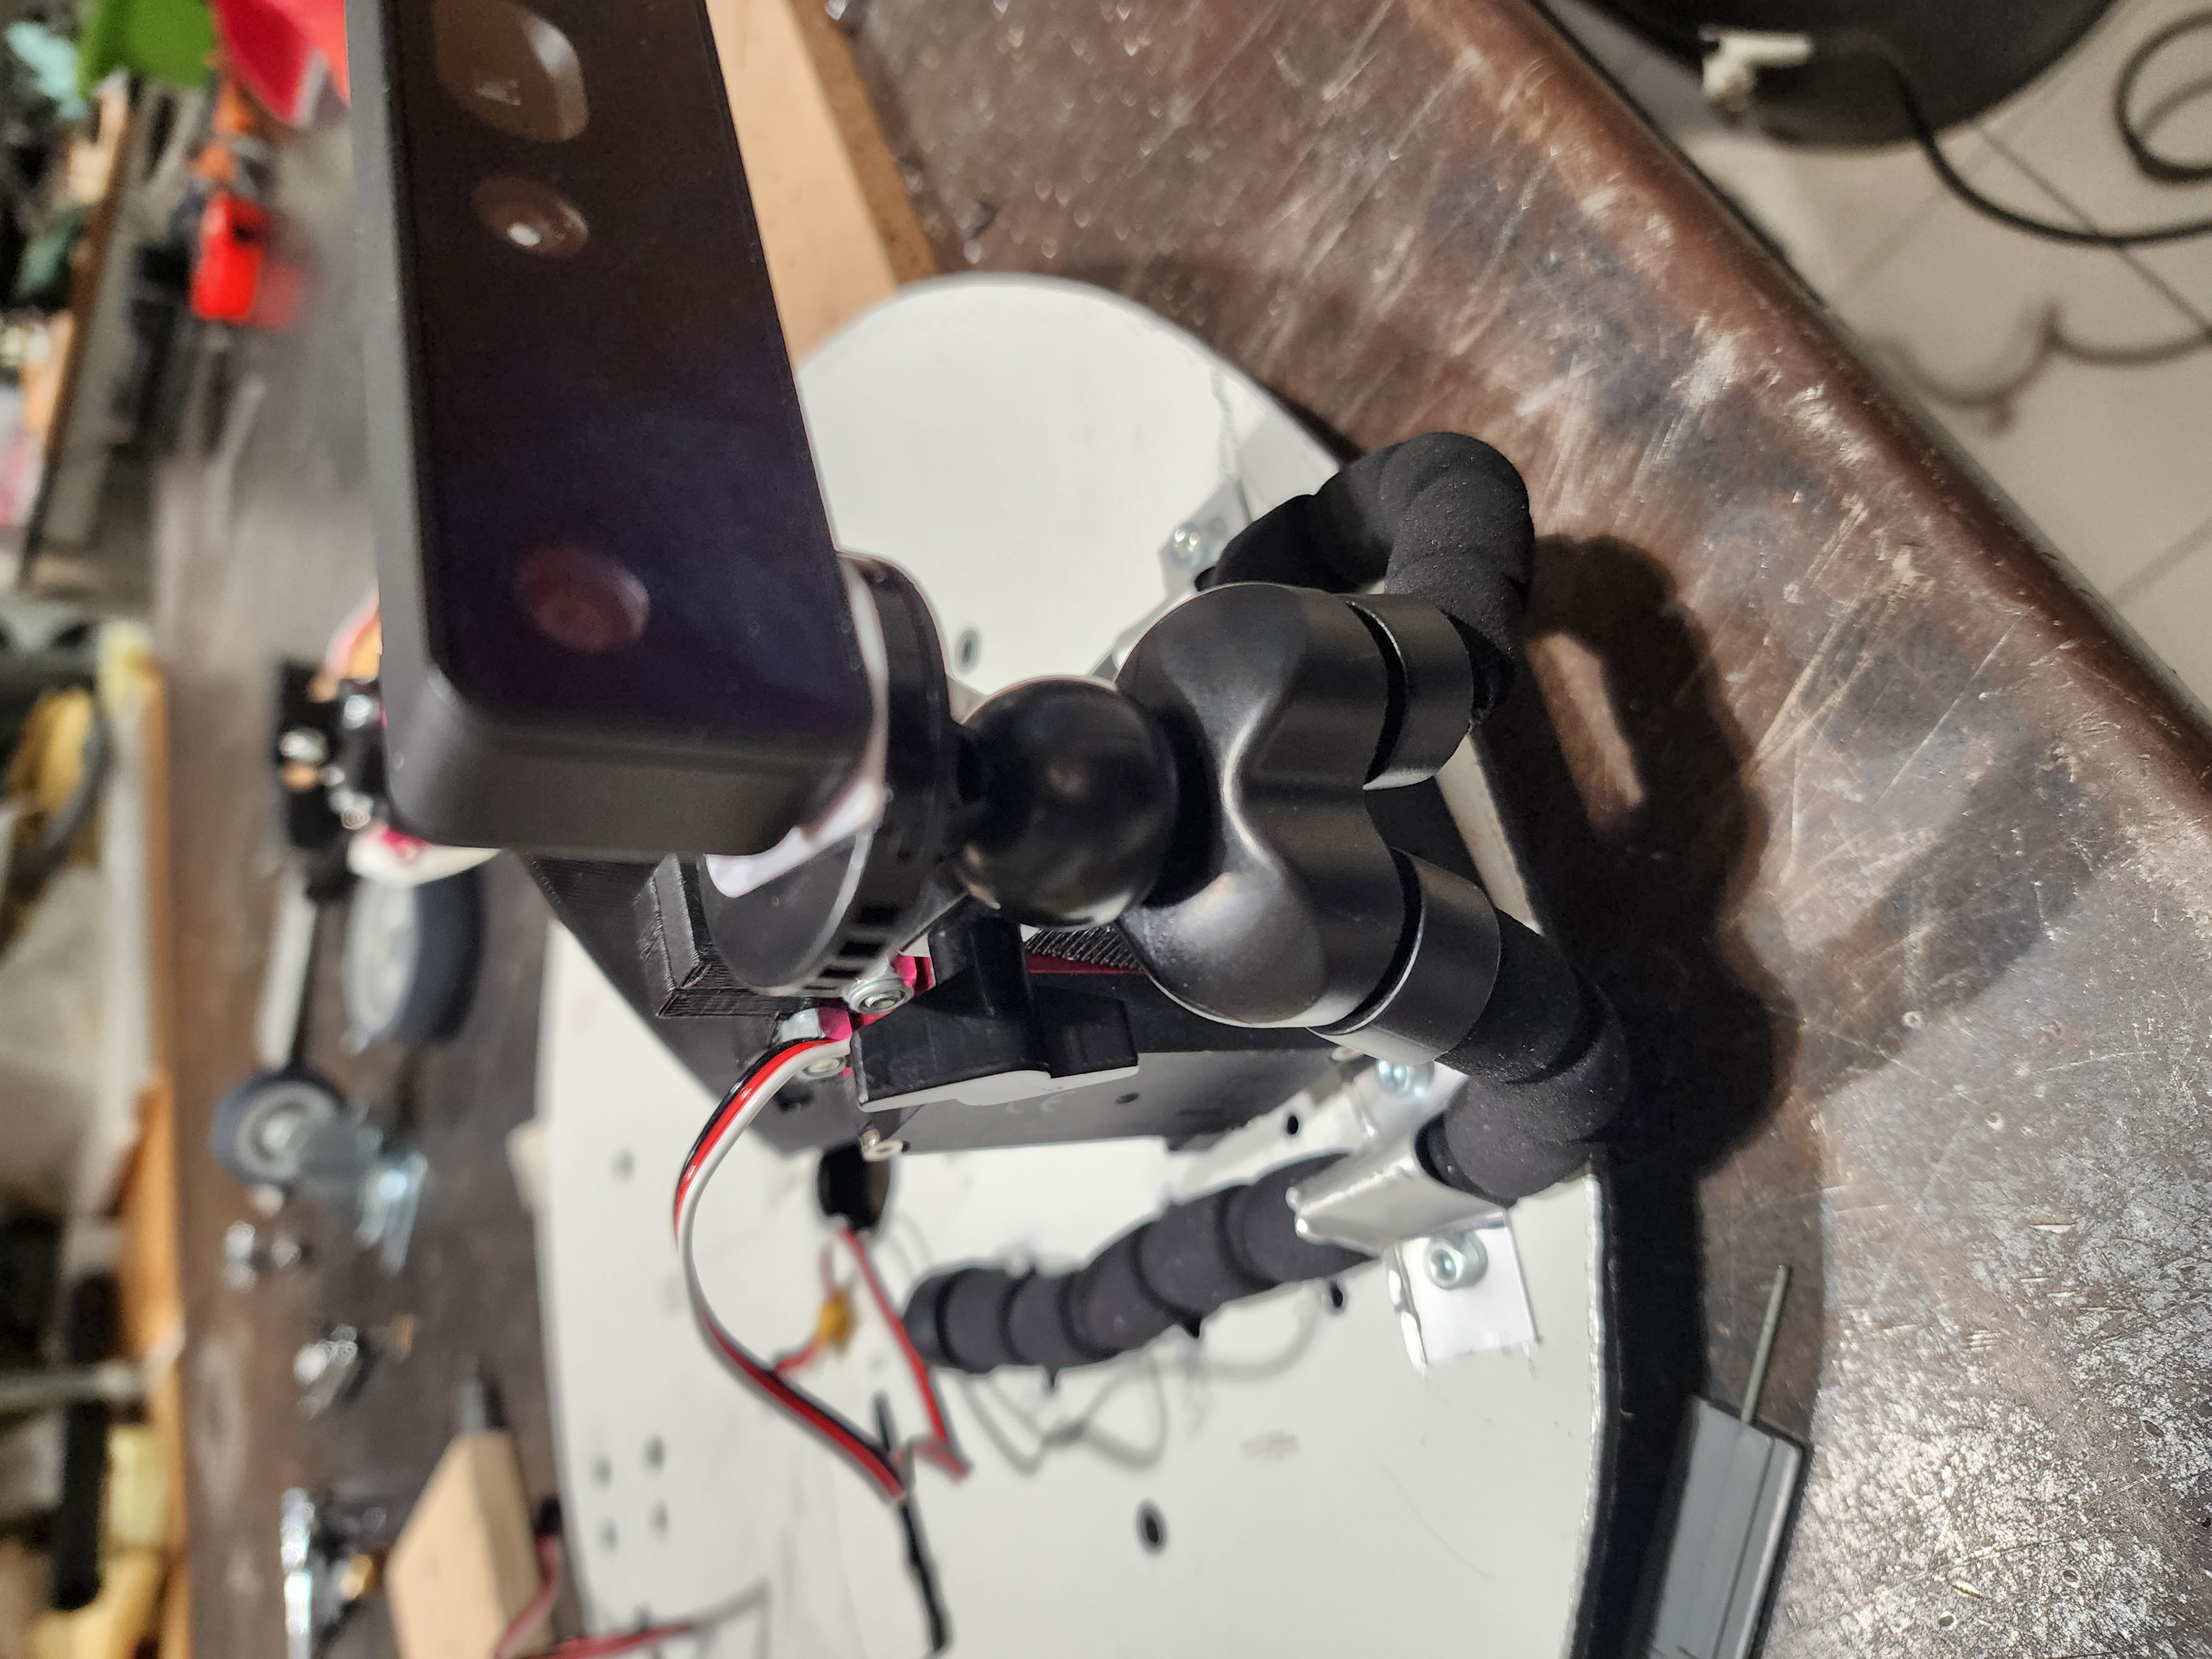
\includegraphics[width=0.6\textwidth, angle=-90]{Images/TripodOnHeadCamera.jpg}
    \caption{Oak-D Pro Camera Mounted on Tripod System}
    \label{fig:tripod_camera_mount}
\end{figure}

The mounting system accommodates the existing servo head geometry while providing secure attachment points for the Oak-D Pro camera, with geometric constraints requiring custom bracket design that works within available space while providing adequate support. Mechanical interfaces utilize standard mounting hardware enabling camera removal for maintenance without requiring bracket system modification.

\begin{figure}[H]
    \centering
    \begin{minipage}{0.45\textwidth}
        \centering
        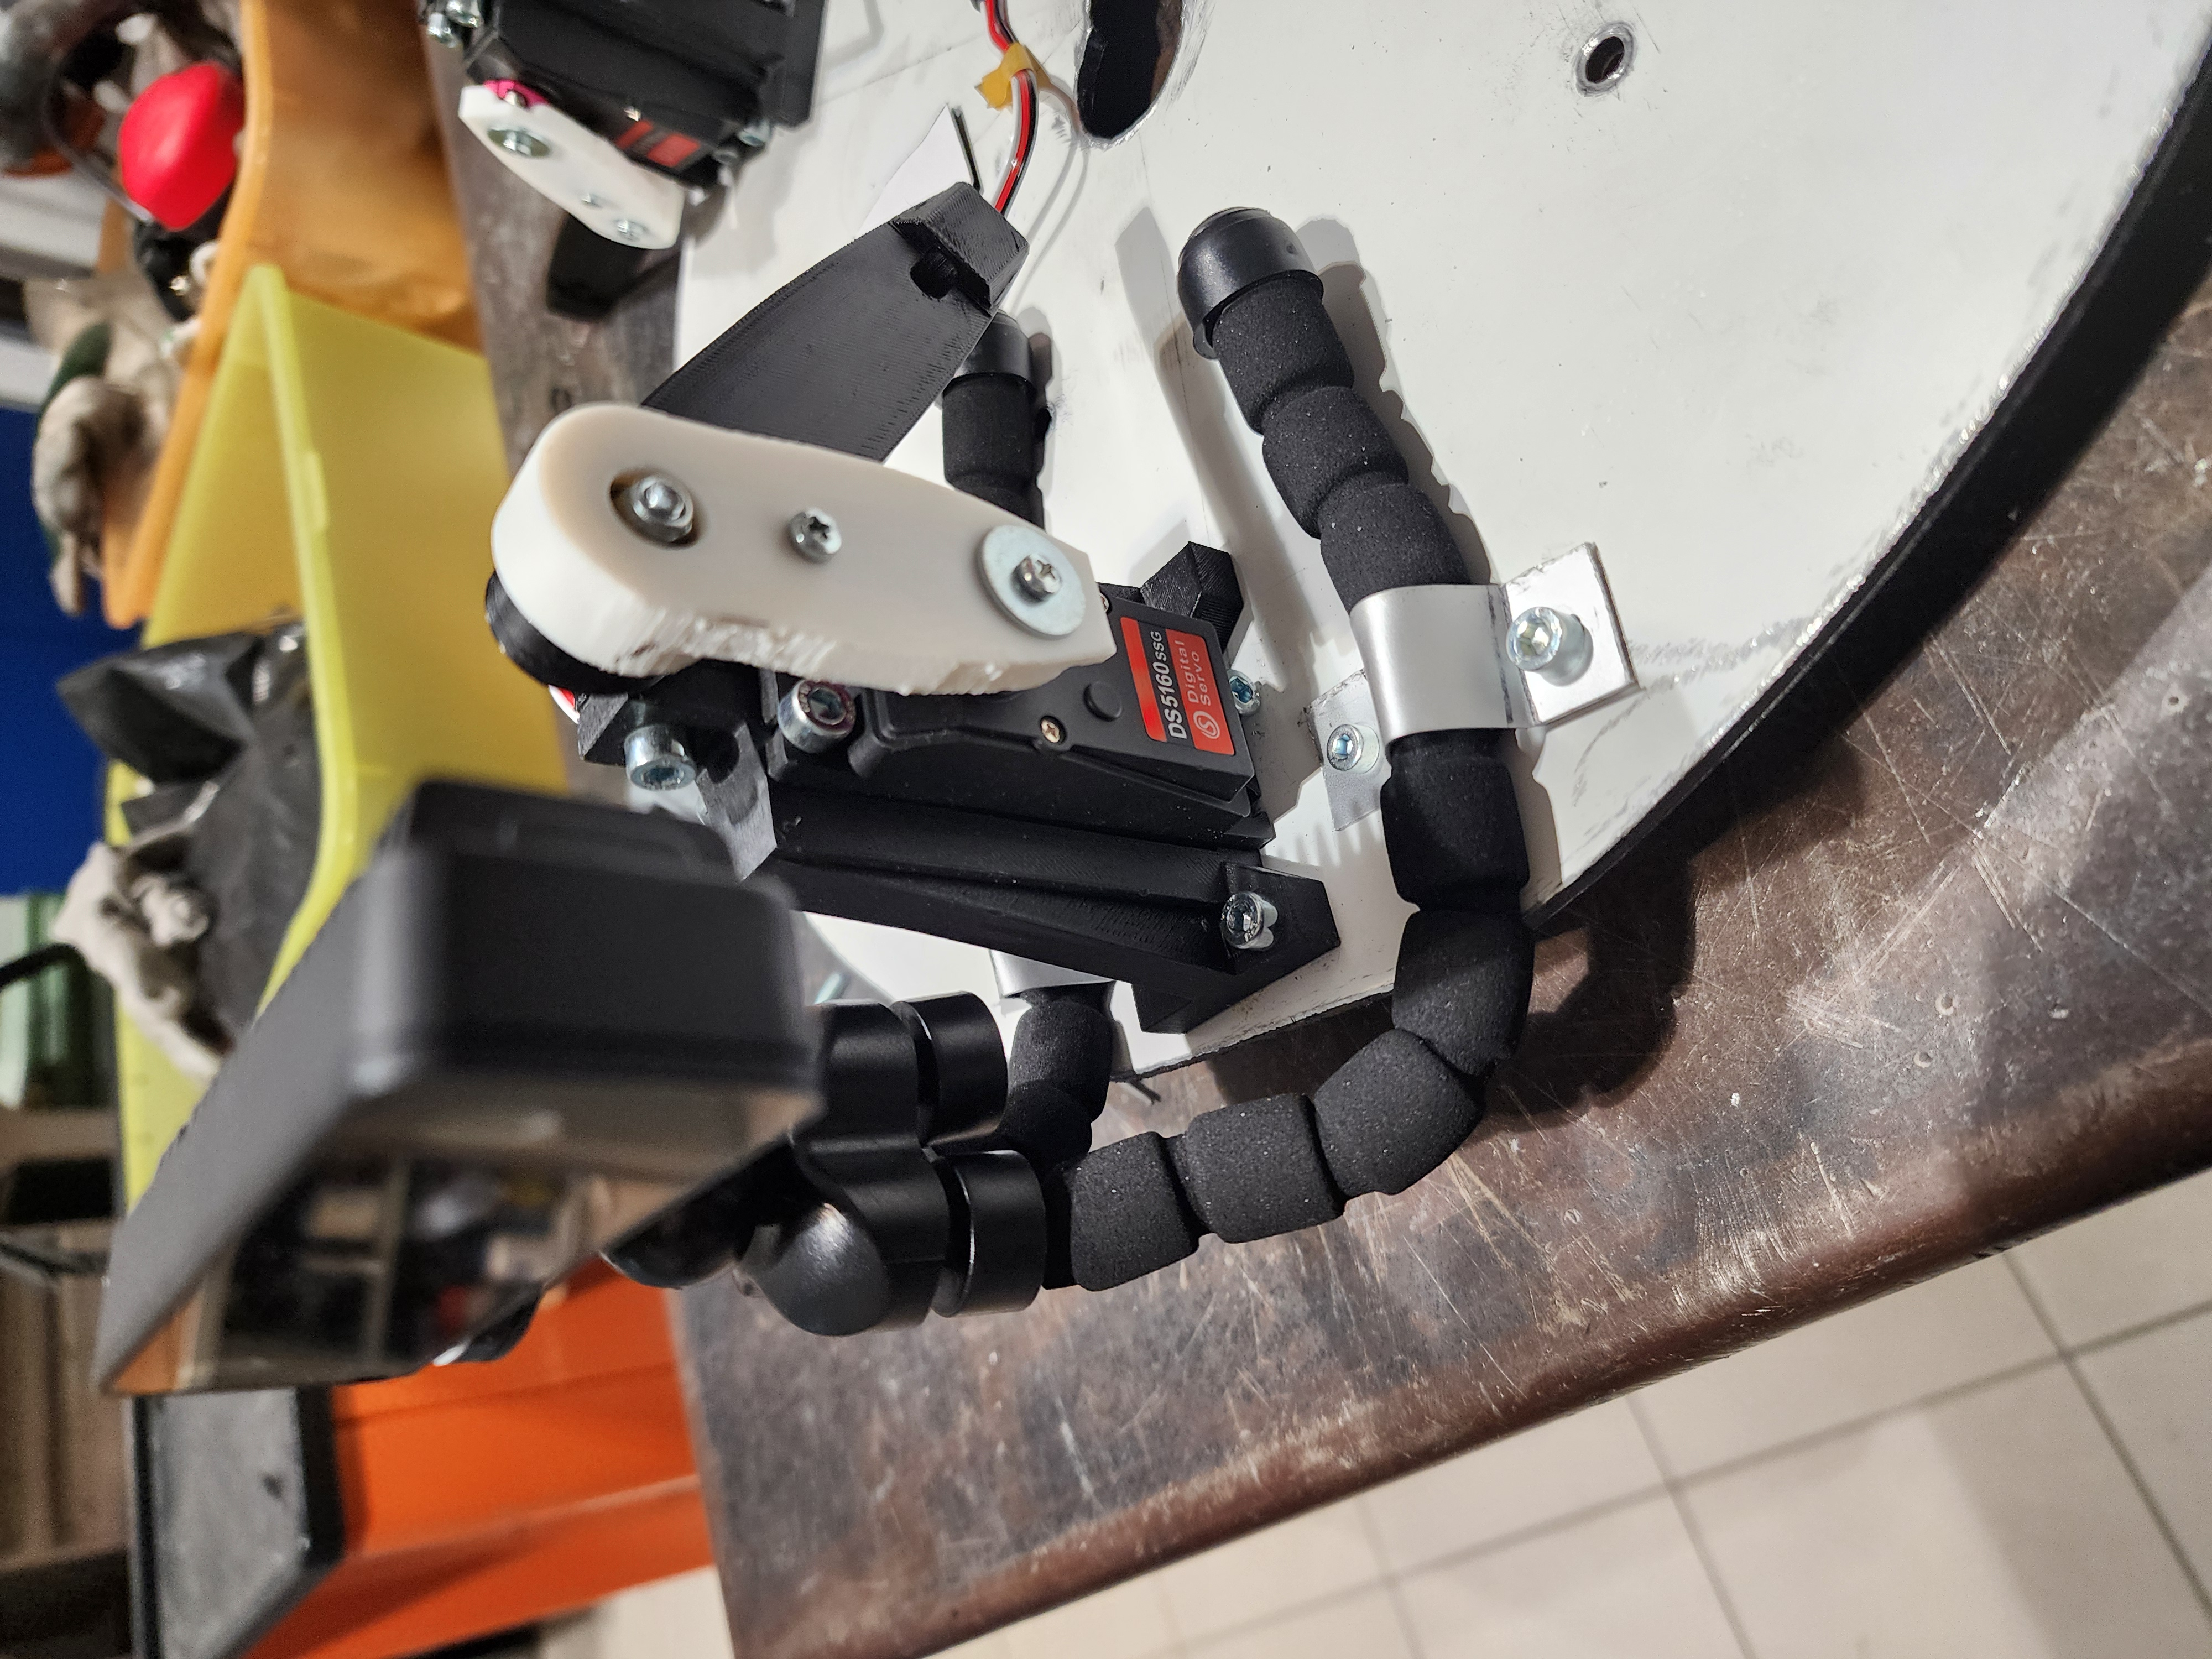
\includegraphics[width=\textwidth, angle=-90]{Images/TripodOnHeadCamera (3).jpg}
        \caption{Oak-D Pro Camera Mounted on Tripod System (Side View)}
        \label{fig:tripod_camera_mount_side}
    \end{minipage}
    \hfill
    \begin{minipage}{0.45\textwidth}
        \centering
        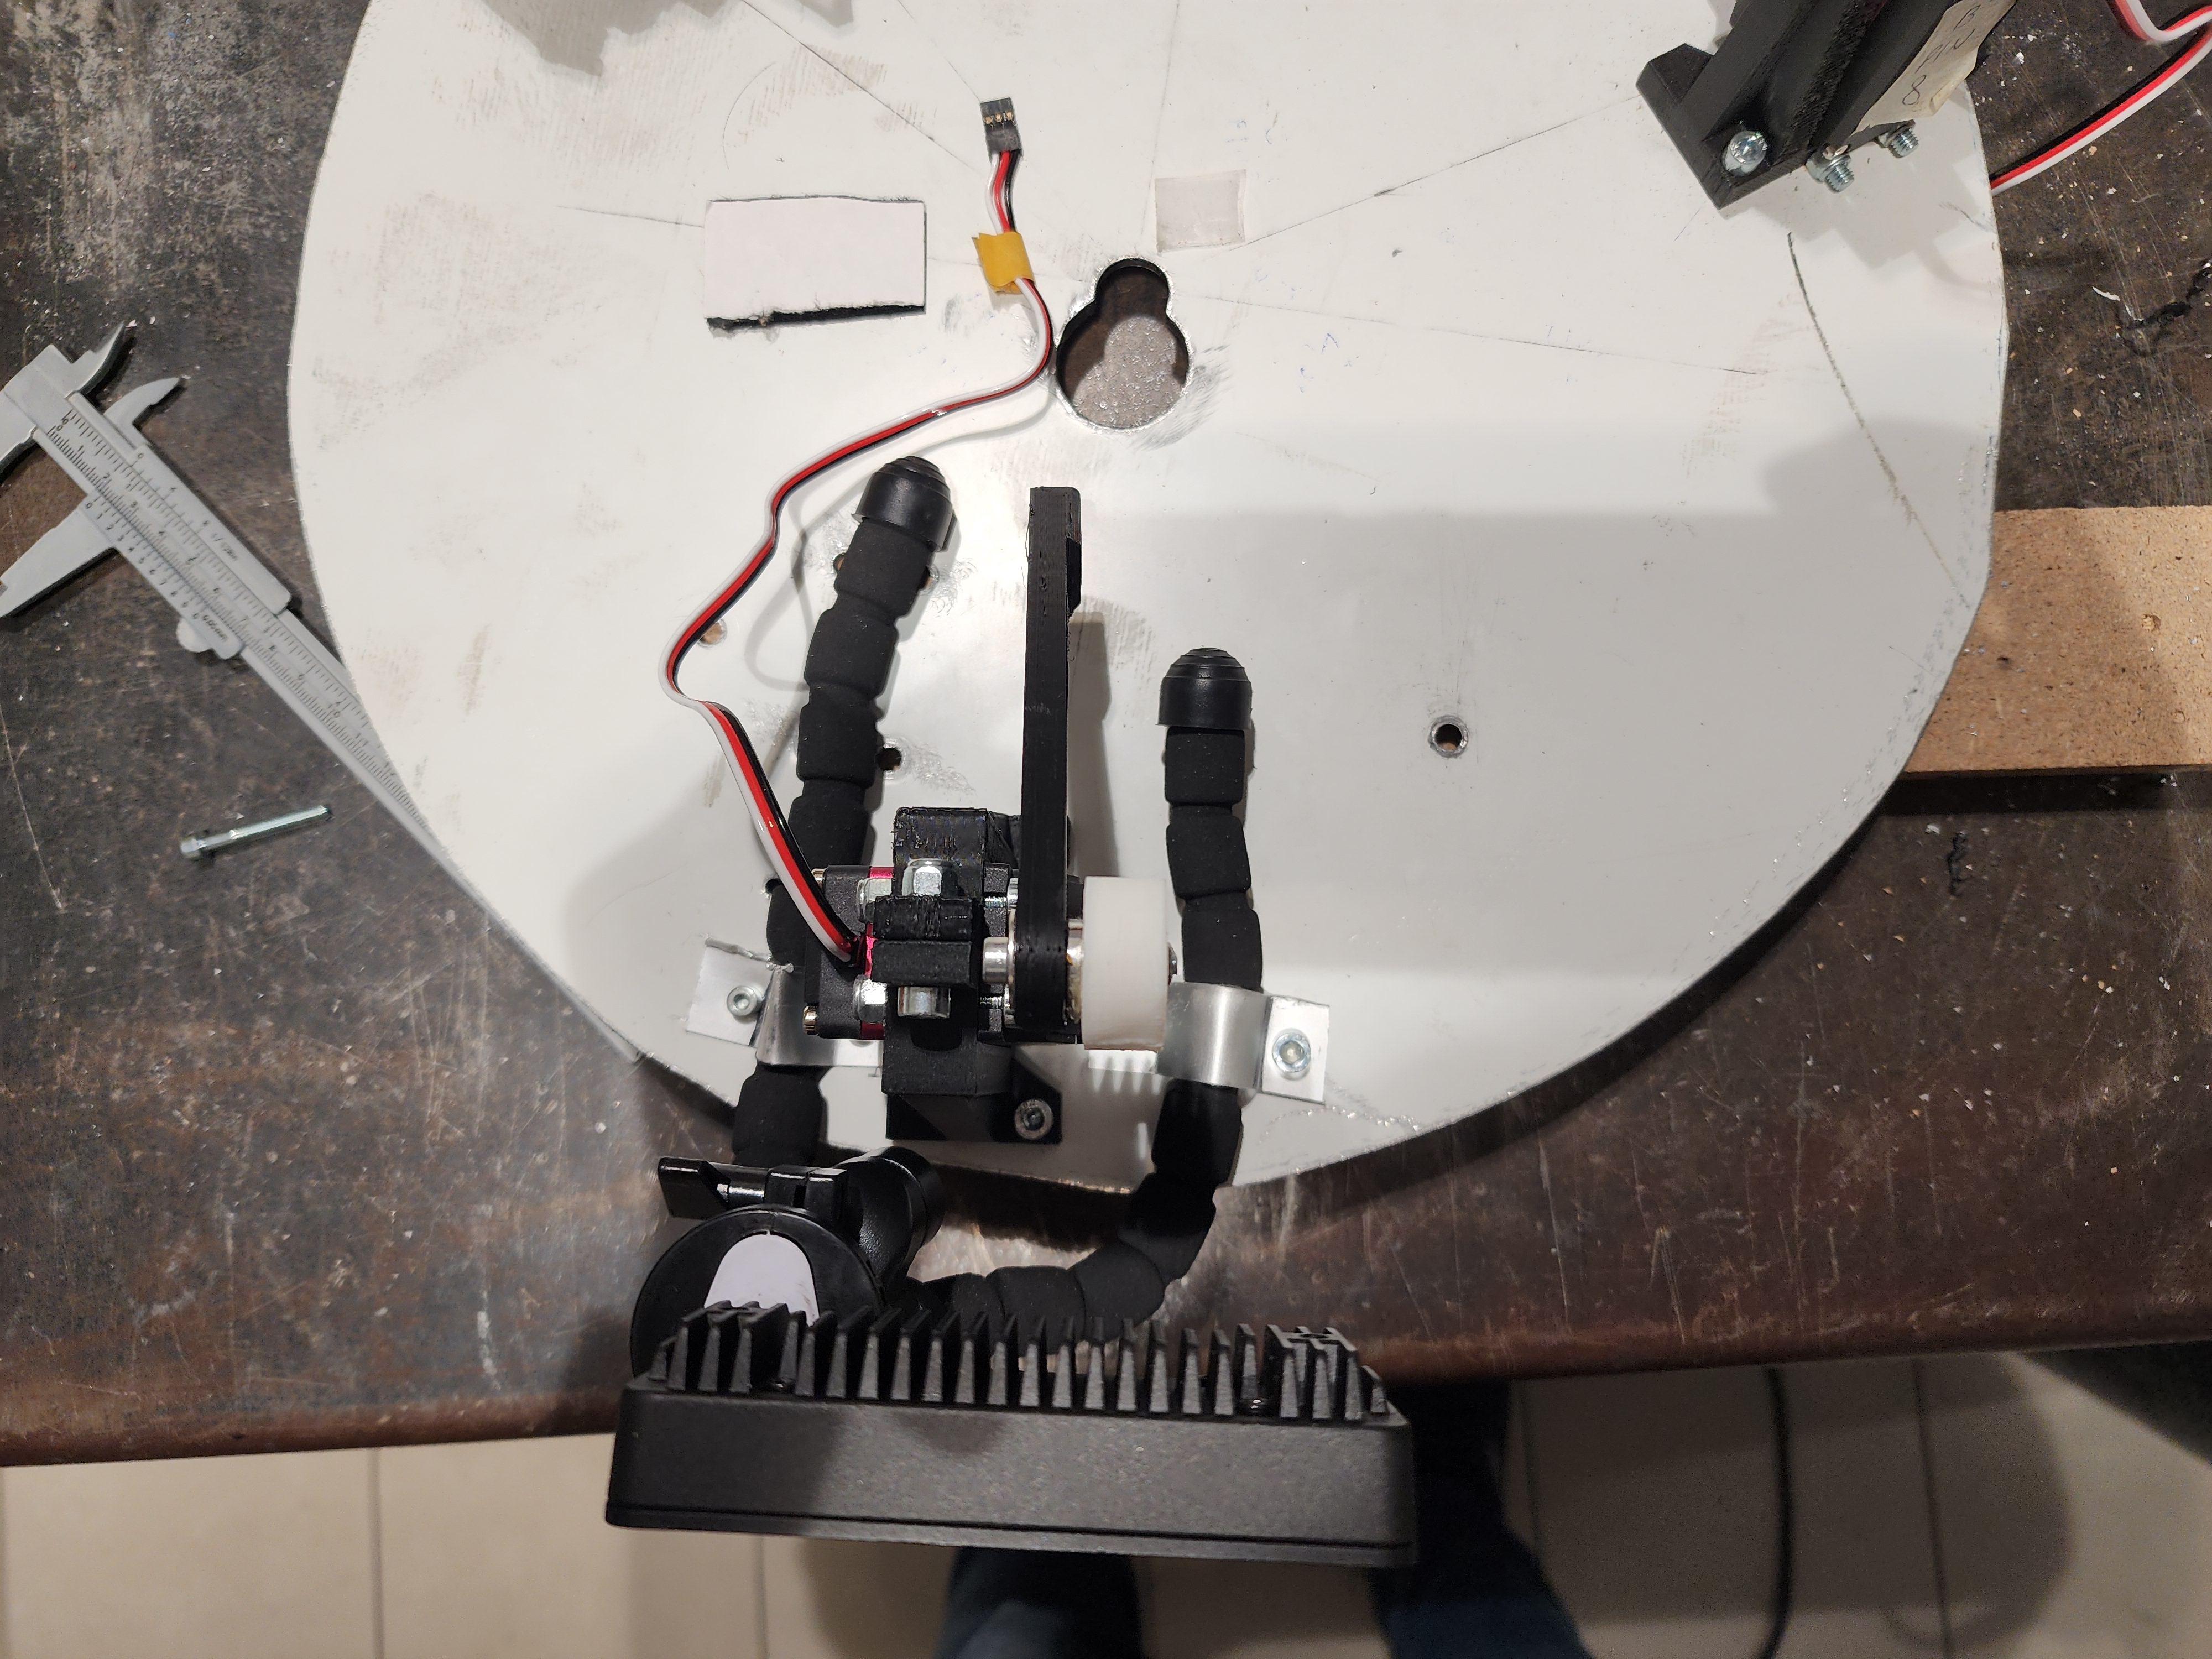
\includegraphics[width=\textwidth]{Images/TripodOnHeadCamera (2).jpg}
        \caption{Oak-D Pro Camera Mounted on Tripod System (Top View)}
        \label{fig:tripod_camera_mount_top}
    \end{minipage}
\end{figure}

\subsubsection{Fabric Integration and Camera Concealment System}

The fabric integration challenge required maintaining camera visibility while preserving Tino's fabric aesthetic and protecting sensitive camera components. Fabric positioning strategies prevent interference with camera sensing through velcro attachment systems that provide secure fabric positioning, preventing fabric drift into camera field of view during operational periods. Testing procedures validate fabric positioning effectiveness under various operational scenarios including head movement, robot locomotion, and extended operational periods.

\begin{figure}[H]
    \centering
    \begin{minipage}{0.45\textwidth}
        \centering
        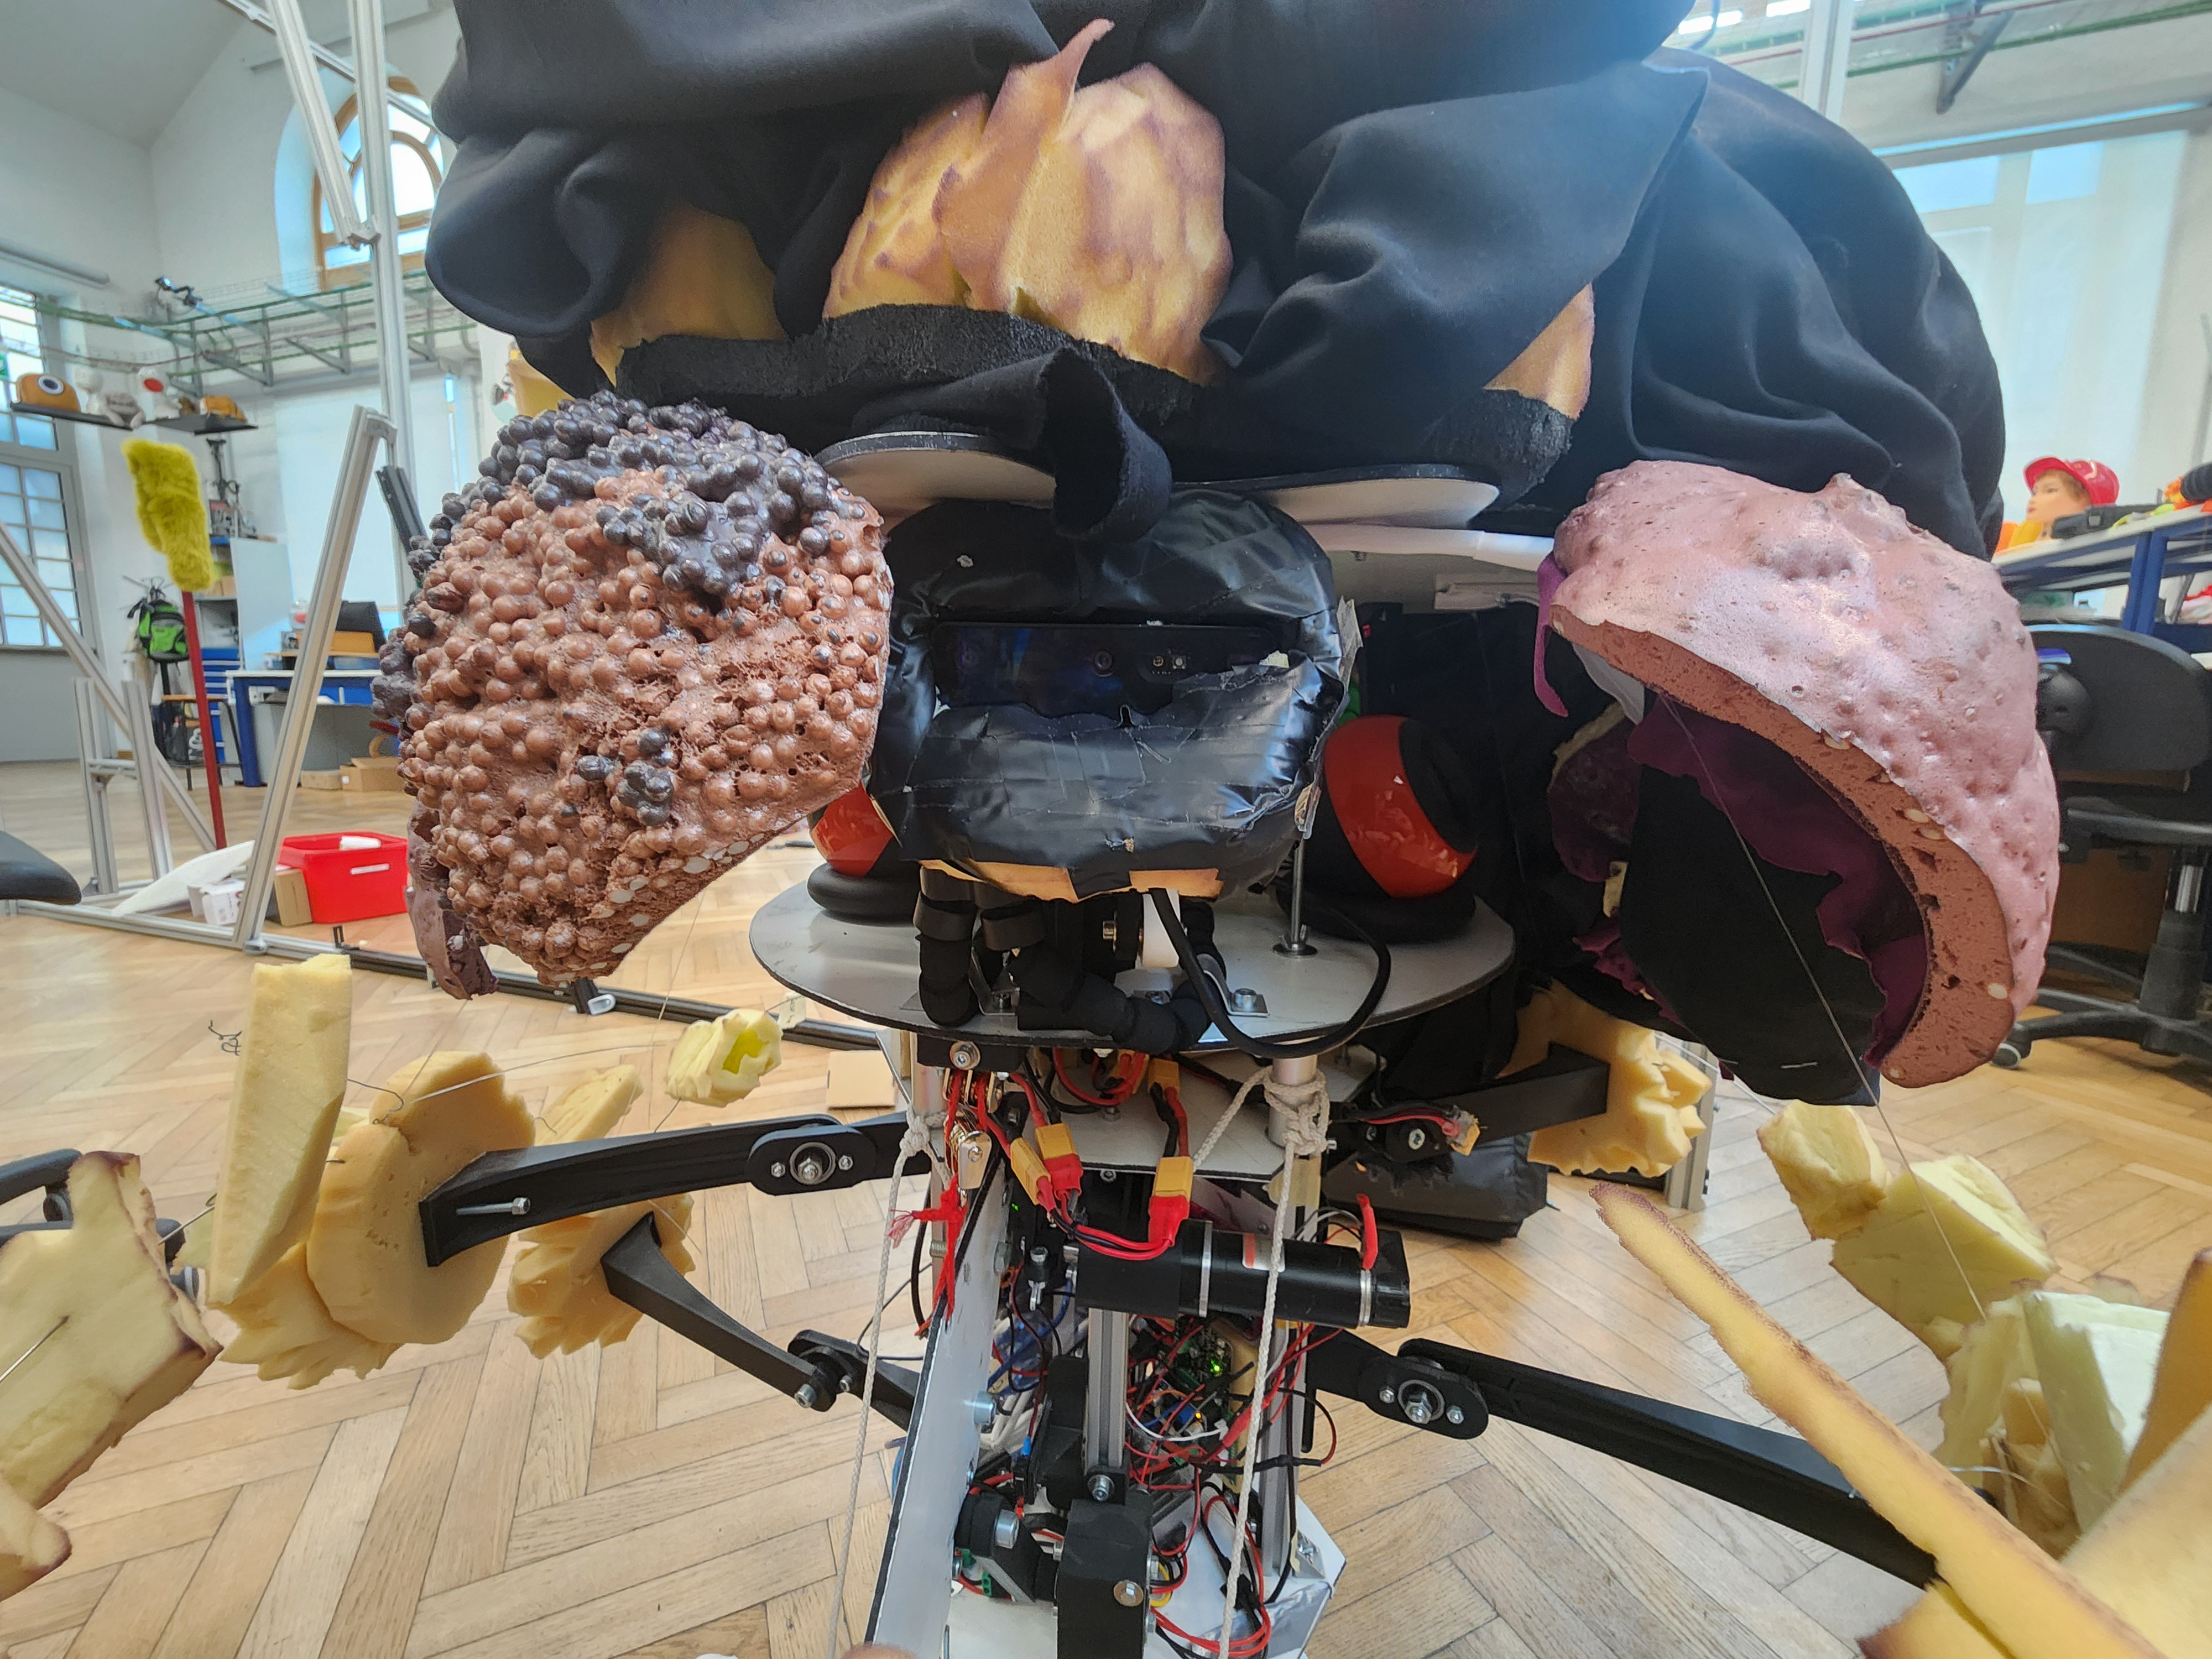
\includegraphics[width=\textwidth]{Images/FirstTryCameraHiding.jpg}
        \caption{Initial Camera Concealment Attempt (Front View)}
        \label{fig:first_try_camera_hiding}
    \end{minipage}
    \hfill
    \begin{minipage}{0.45\textwidth}
        \centering
        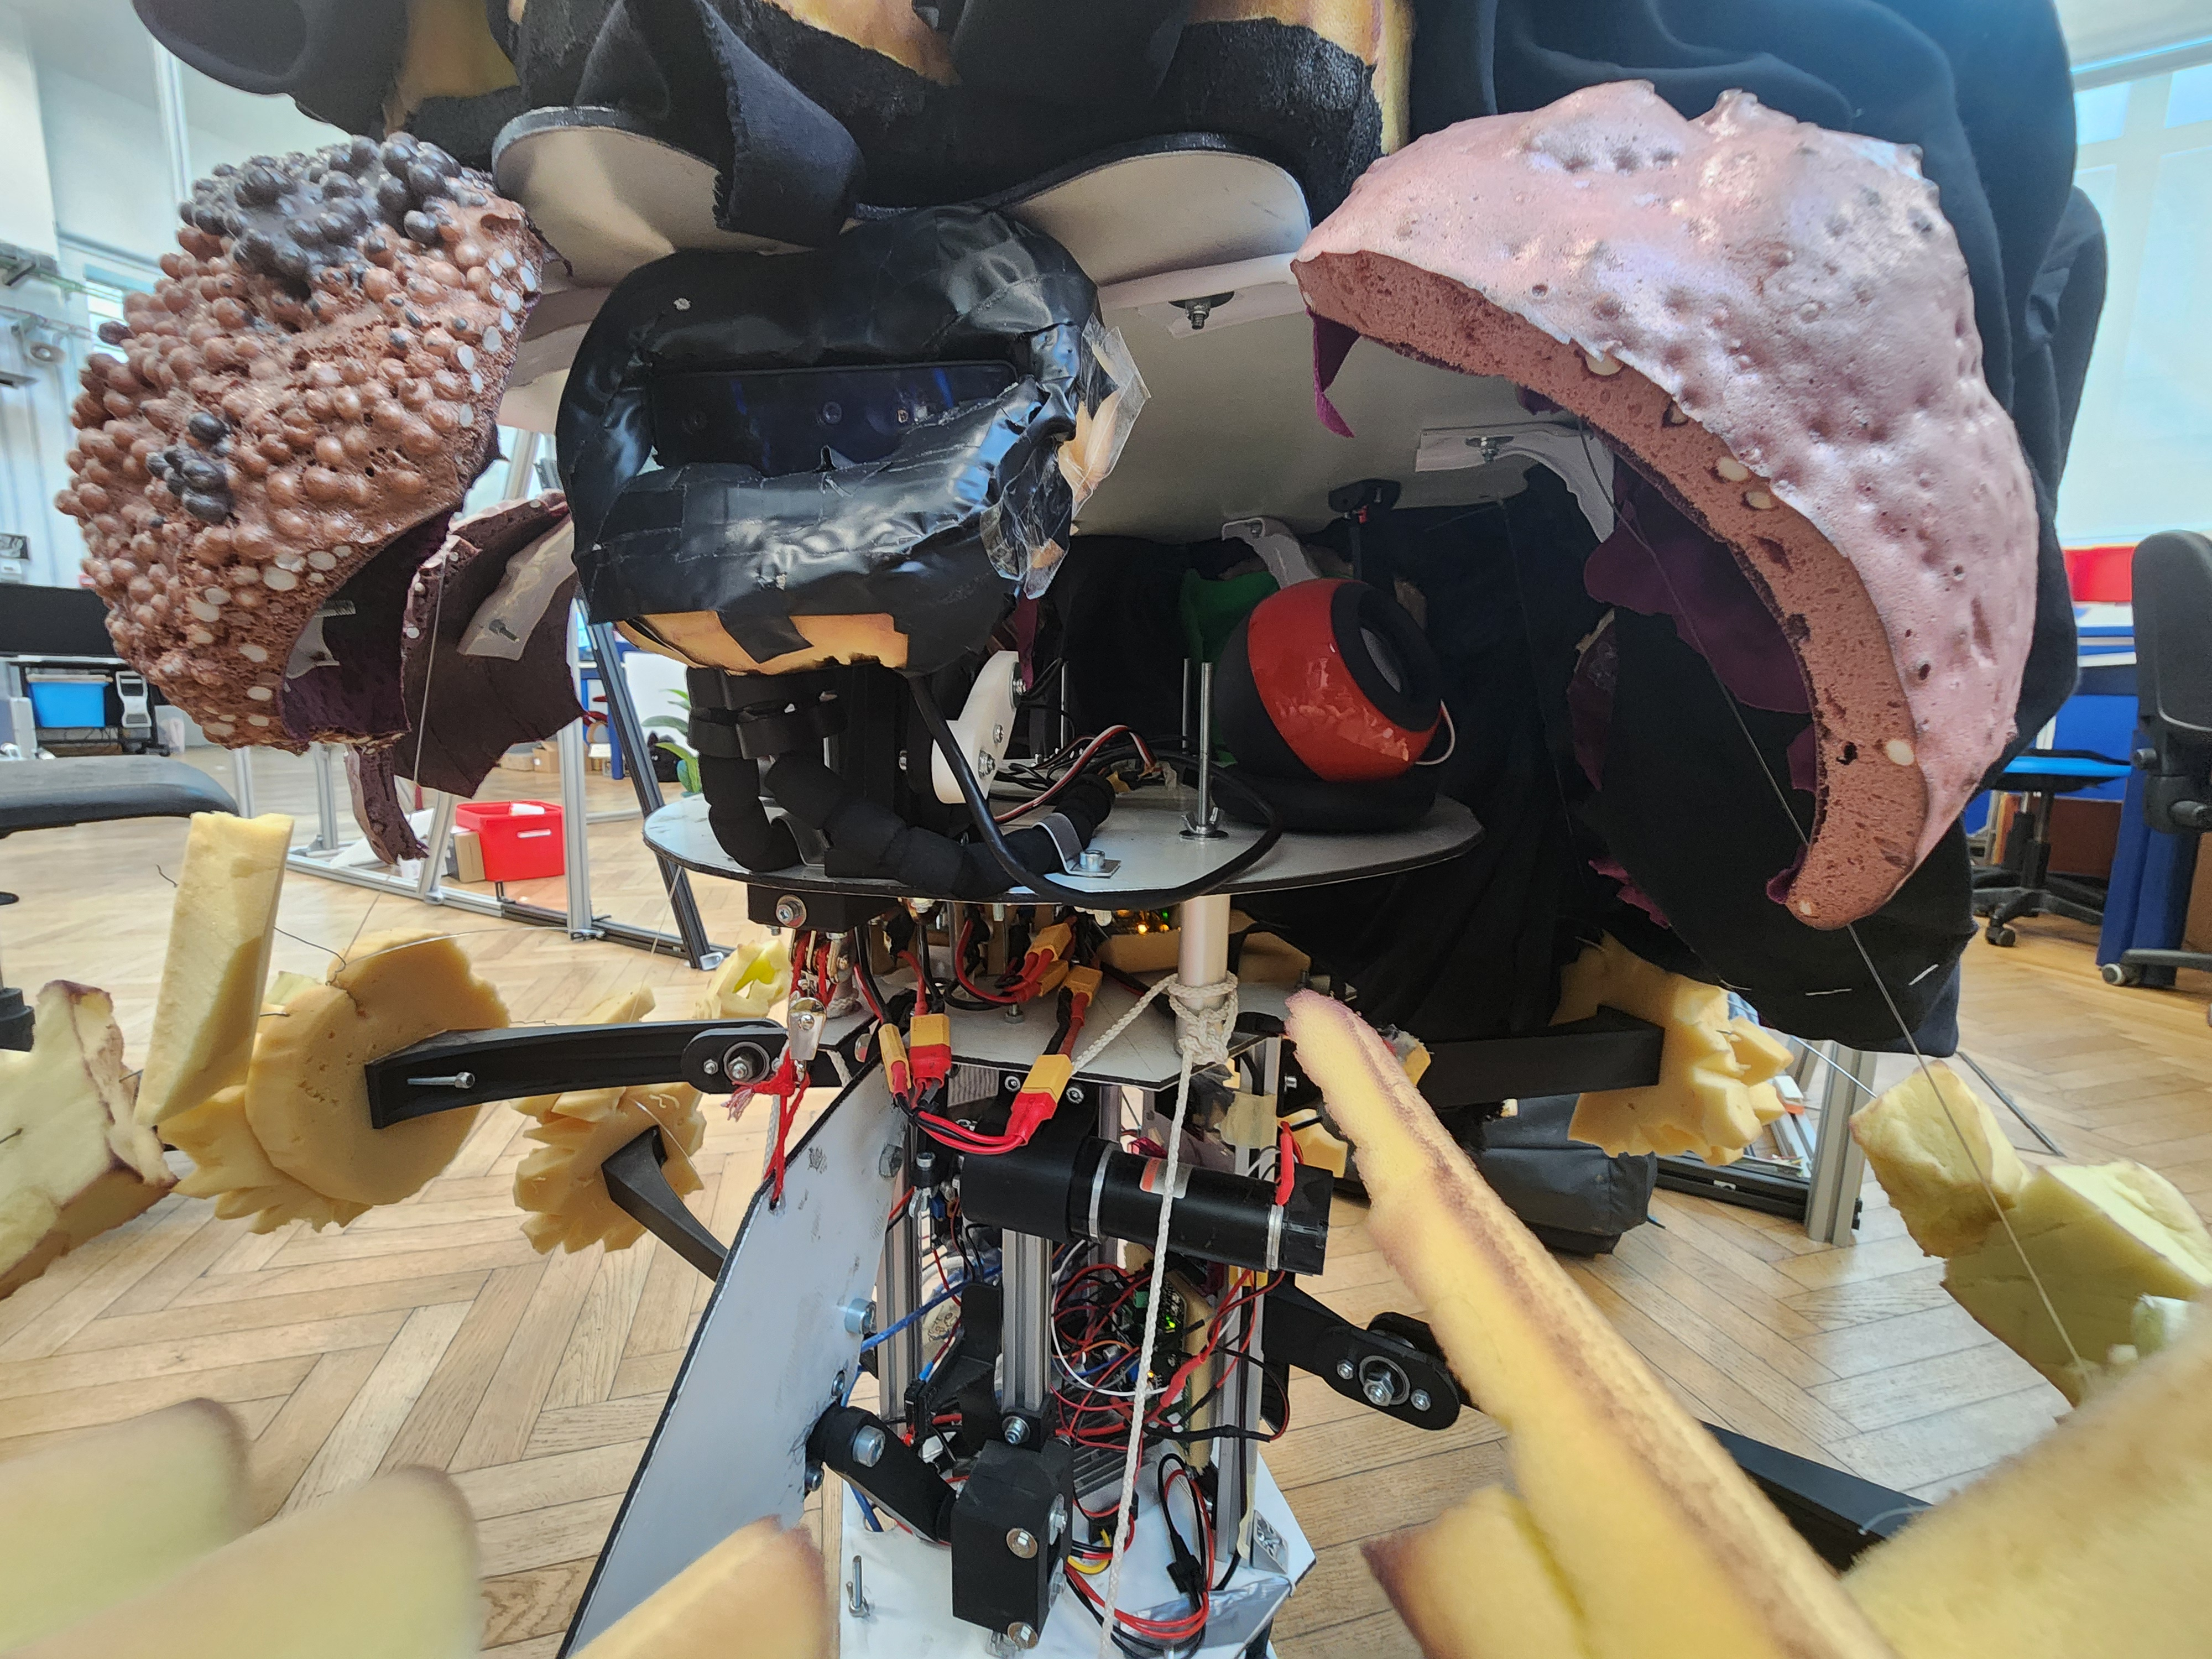
\includegraphics[width=\textwidth]{Images/FirstTryCameraHiding (3).jpg}
        \caption{Initial Camera Concealment Attempt (Side View)}
        \label{fig:camera_hiding_mesh}
    \end{minipage}
\end{figure}

The comprehensive camera shell system provides protection and fabric integration while maintaining optimal camera performance and heat dissipation characteristics. The custom shell design provides camera protection through strategic ventilation openings that enable heat dissipation without compromising environmental protection, with shell geometry optimizing airflow characteristics while minimizing dust ingress.

\begin{figure}[H]
    \centering
    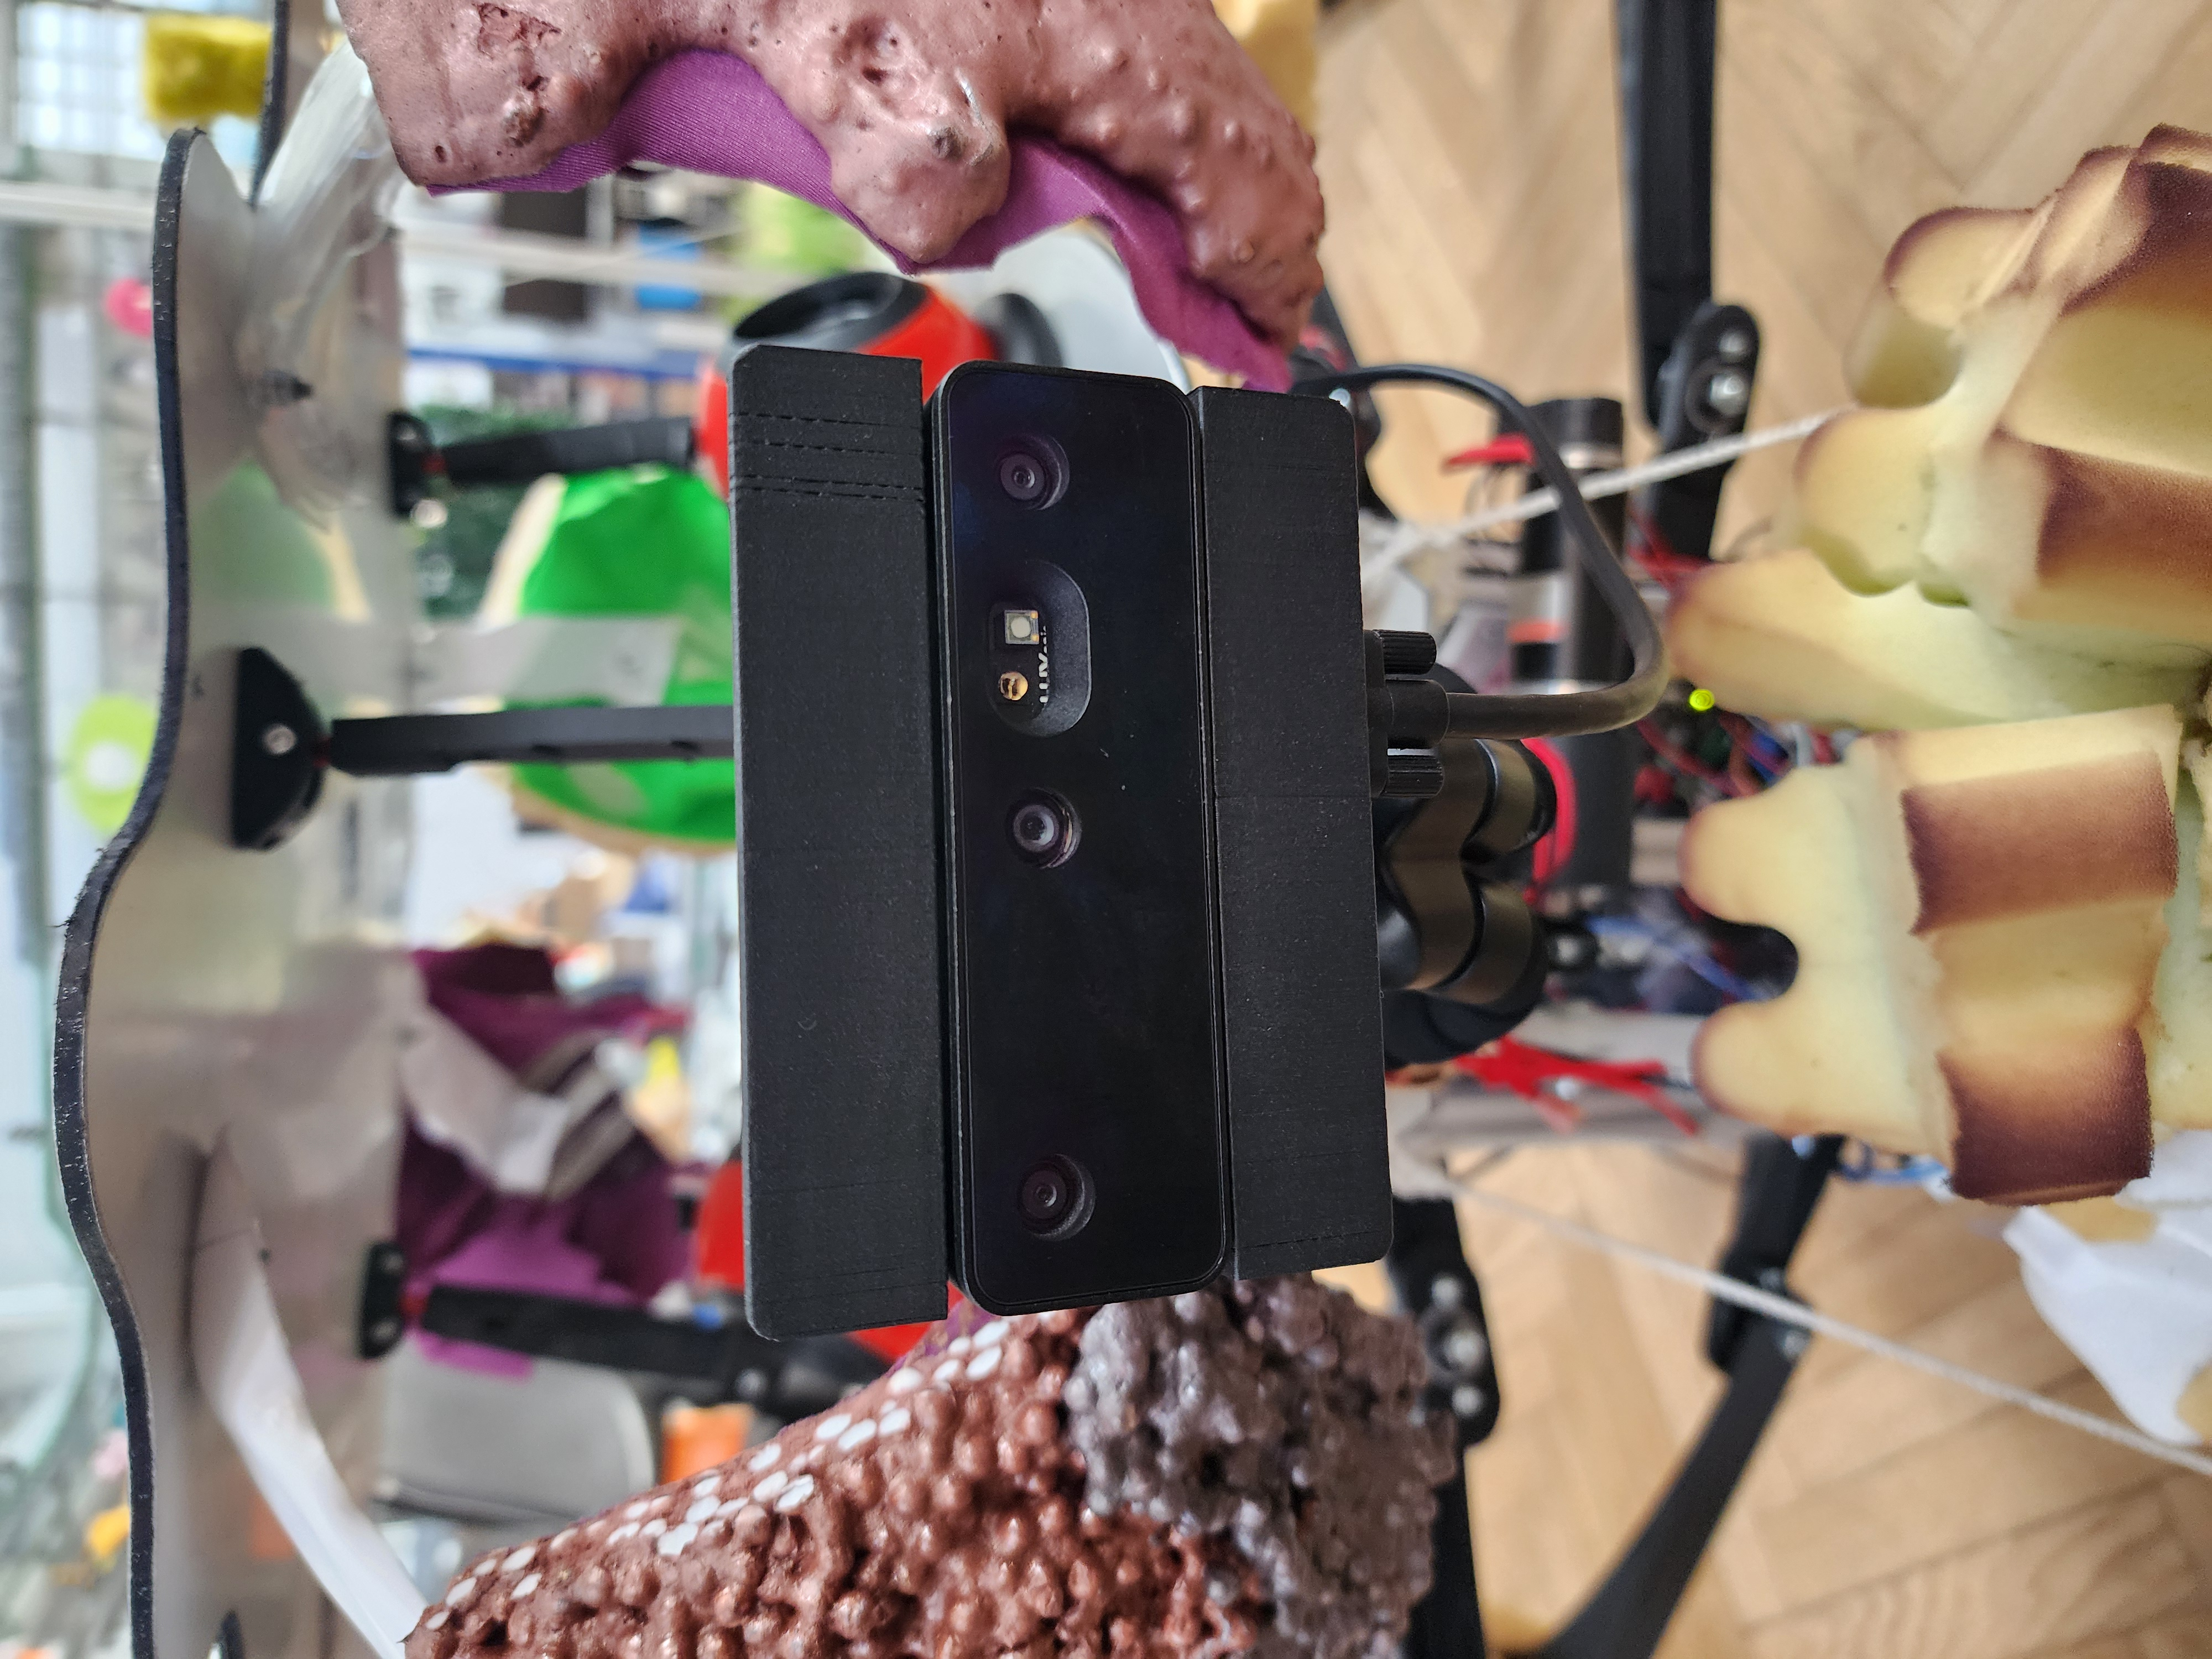
\includegraphics[height=8cm, angle=-90]{Images/CameraCasingNoMesh.jpg}
    \caption{Camera Casing without Mesh Covering}
    \label{fig:camera_casing_no_mesh}
\end{figure}

Attachment integration with the tripod mounting system provides secure shell mounting that enables camera access for maintenance while providing operational protection. Thermal management considerations ensure adequate heat dissipation during extended operation periods, particularly during high-resolution stereo processing that generates significant thermal loads.

\begin{figure}[H]
    \centering
    \begin{minipage}{0.45\textwidth}
        \centering
        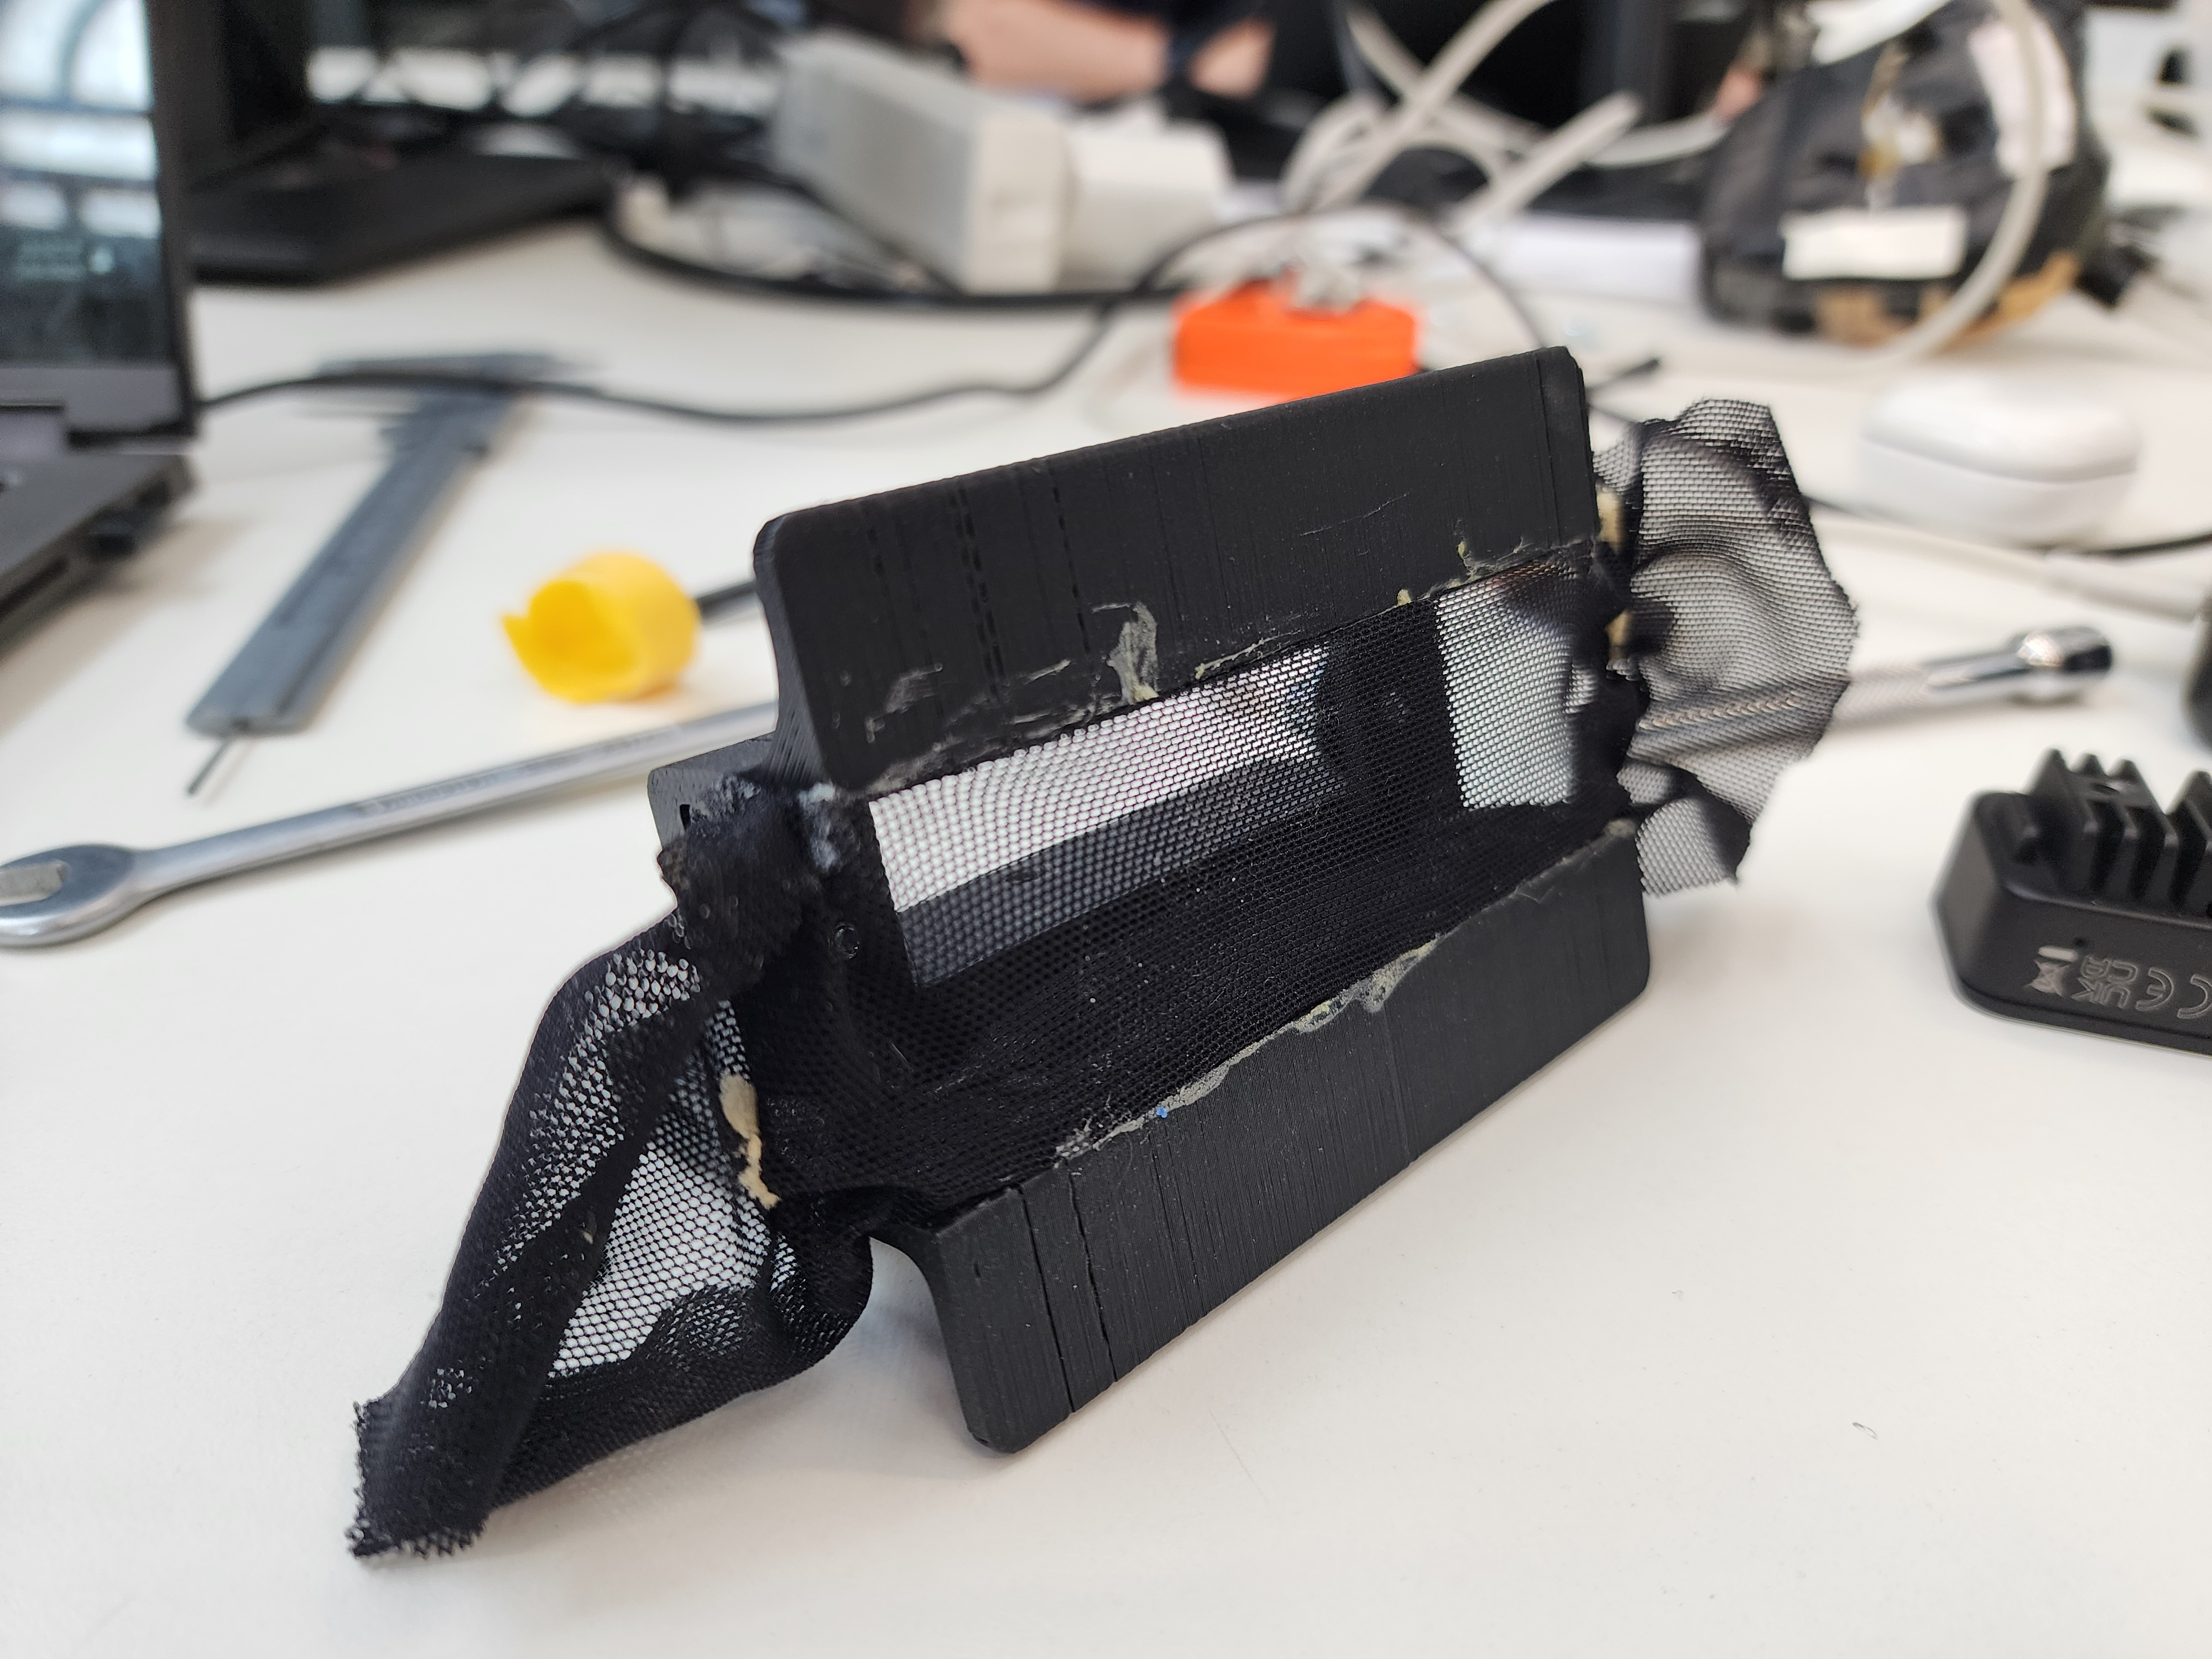
\includegraphics[width=0.8\textwidth]{Images/CameraCasingMesh.jpg}
        \caption{Camera Casing with Mesh Covering (No camera)} 
        \label{fig:camera_casing_mesh}
    \end{minipage}
    \hfill
    \begin{minipage}{0.45\textwidth}
        \centering
        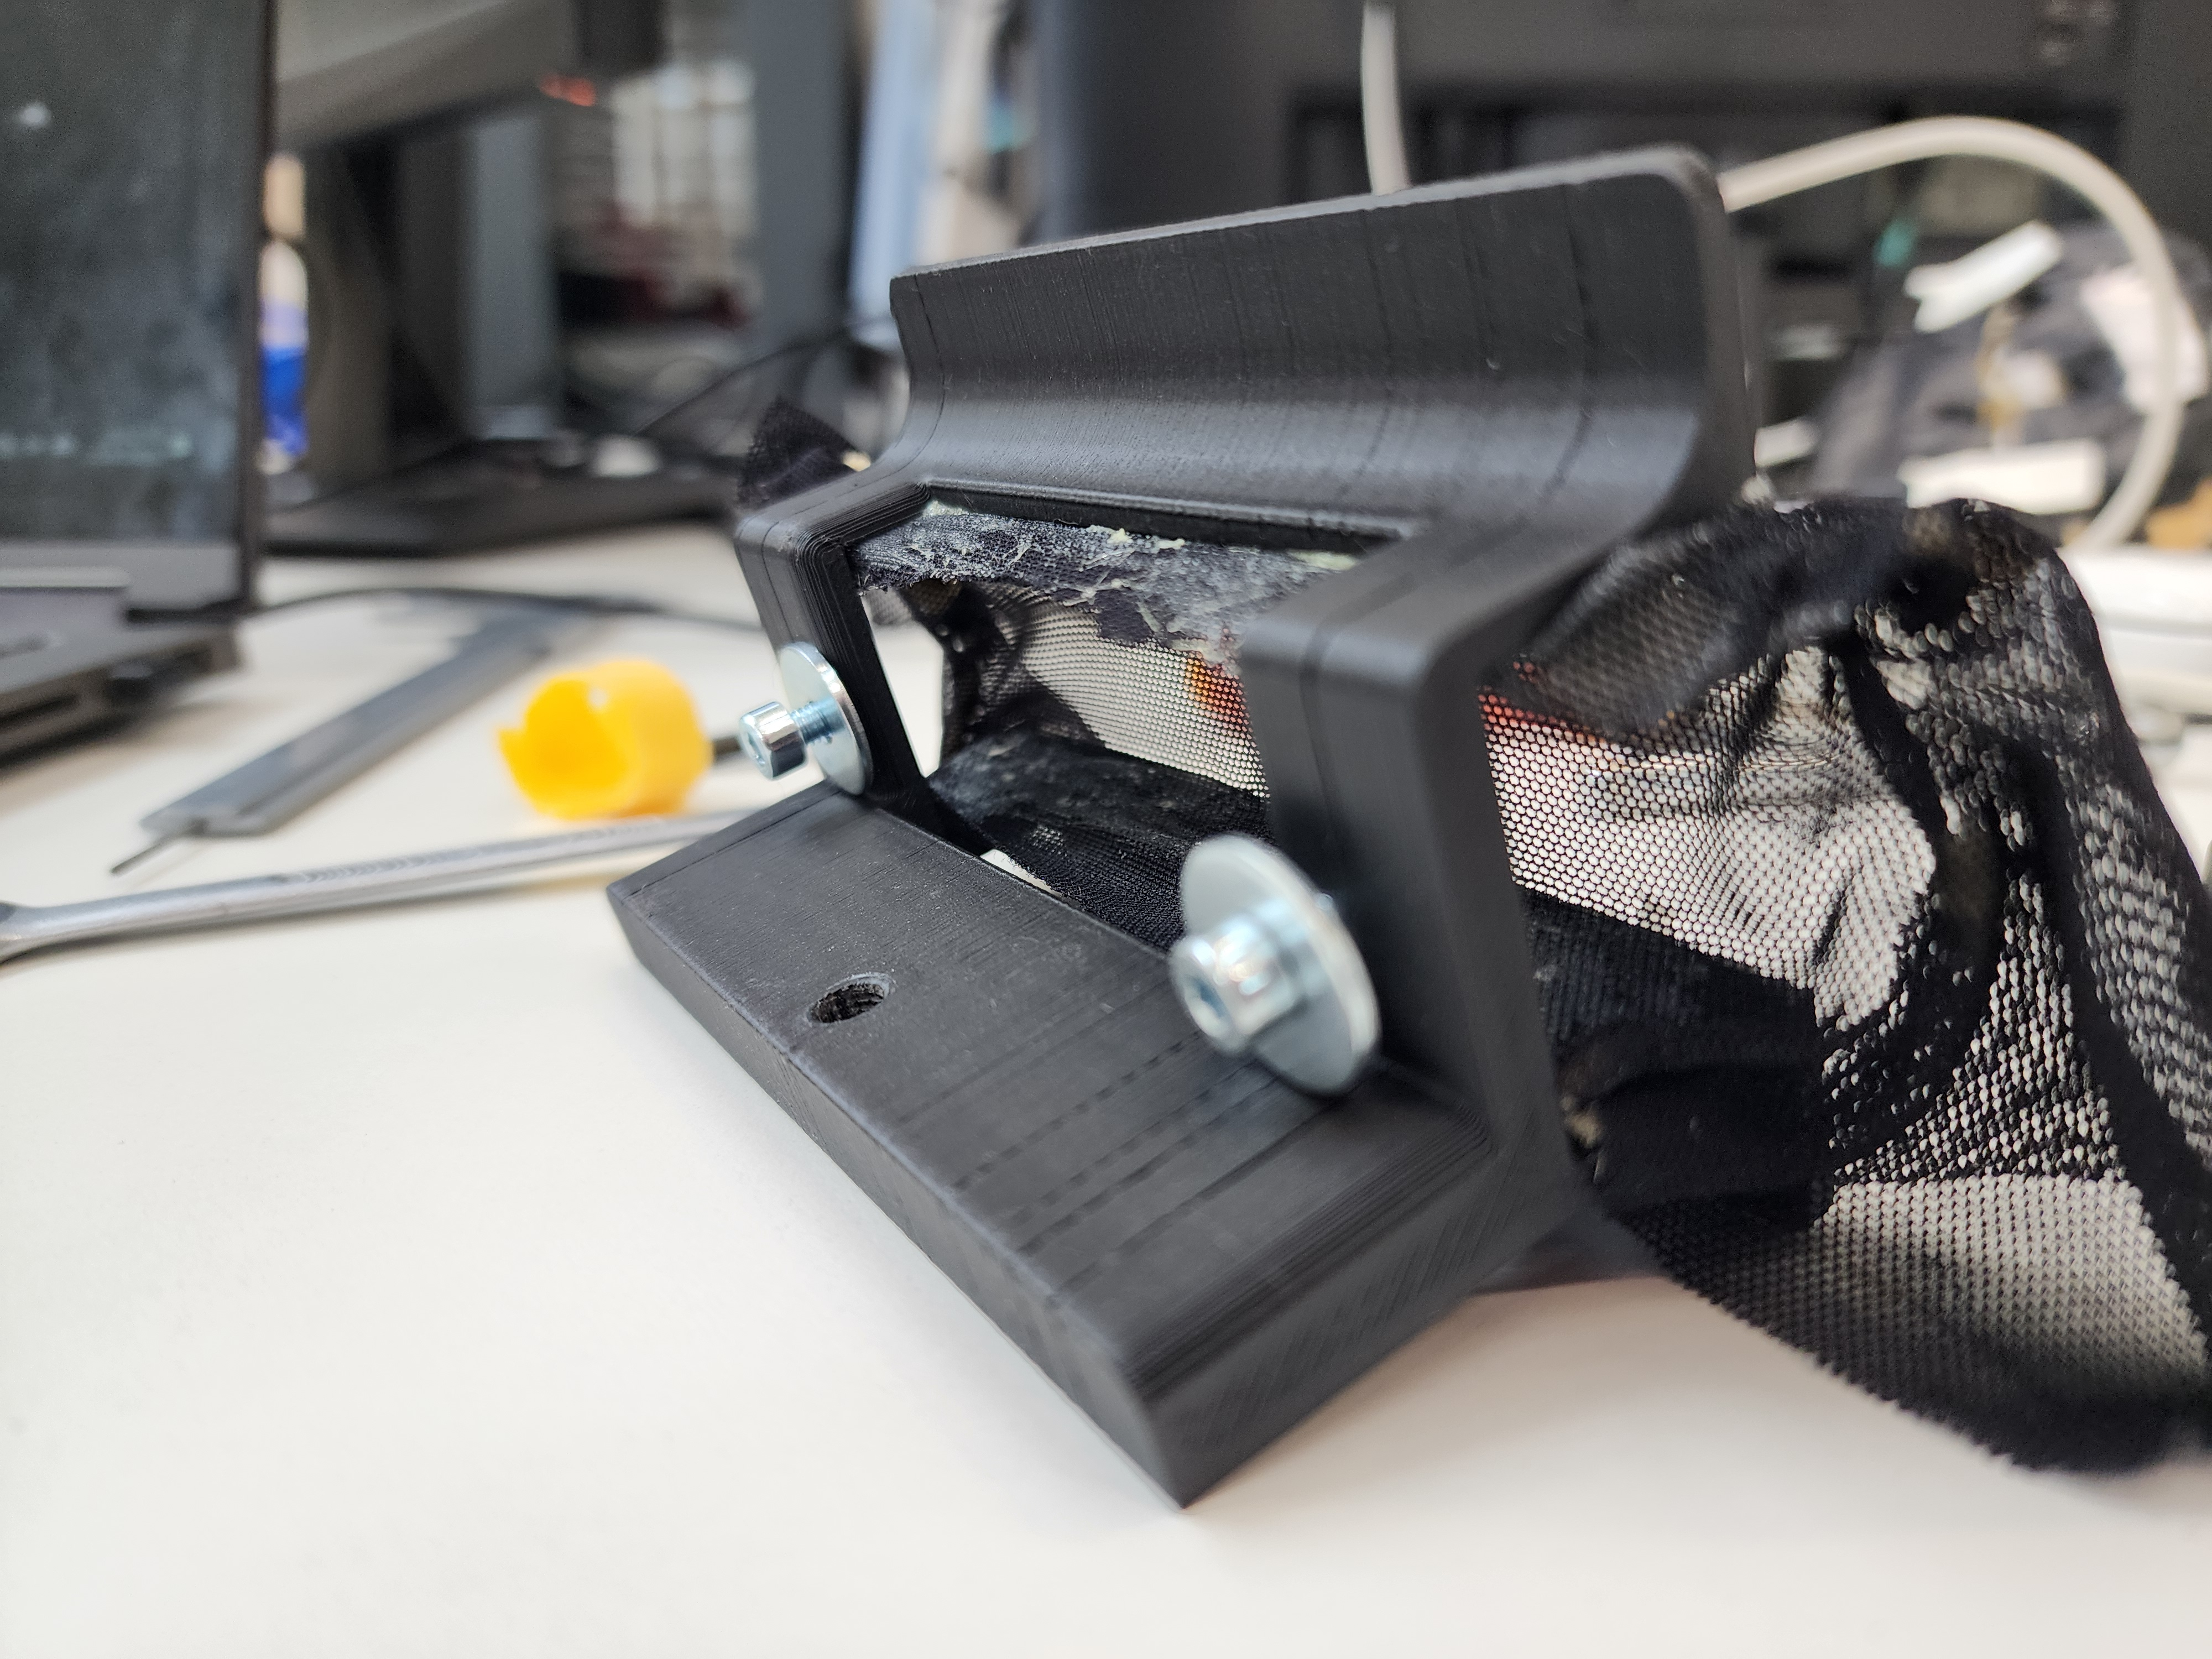
\includegraphics[width=0.8\textwidth]{Images/CameraCasingMesh (2).jpg}
        \caption{Camera Casing with Mesh Covering (No camera)}
        \label{fig:camera_casing_mesh_back}
    \end{minipage}
\end{figure}

The fabric control system utilizes velcro attachments integrated with shell flaps to provide positive fabric positioning control, with velcro implementation including both shell-mounted components and fabric-sewn counterparts that provide reliable attachment while enabling fabric removal for maintenance. Mesh covering implementation conceals camera presence from casual observation while maintaining full optical transmission characteristics, with optical testing validating maintained image quality and depth sensing performance through the concealment system.

\begin{figure}[H]
    \centering
    \begin{minipage}{0.45\textwidth}
        \centering
        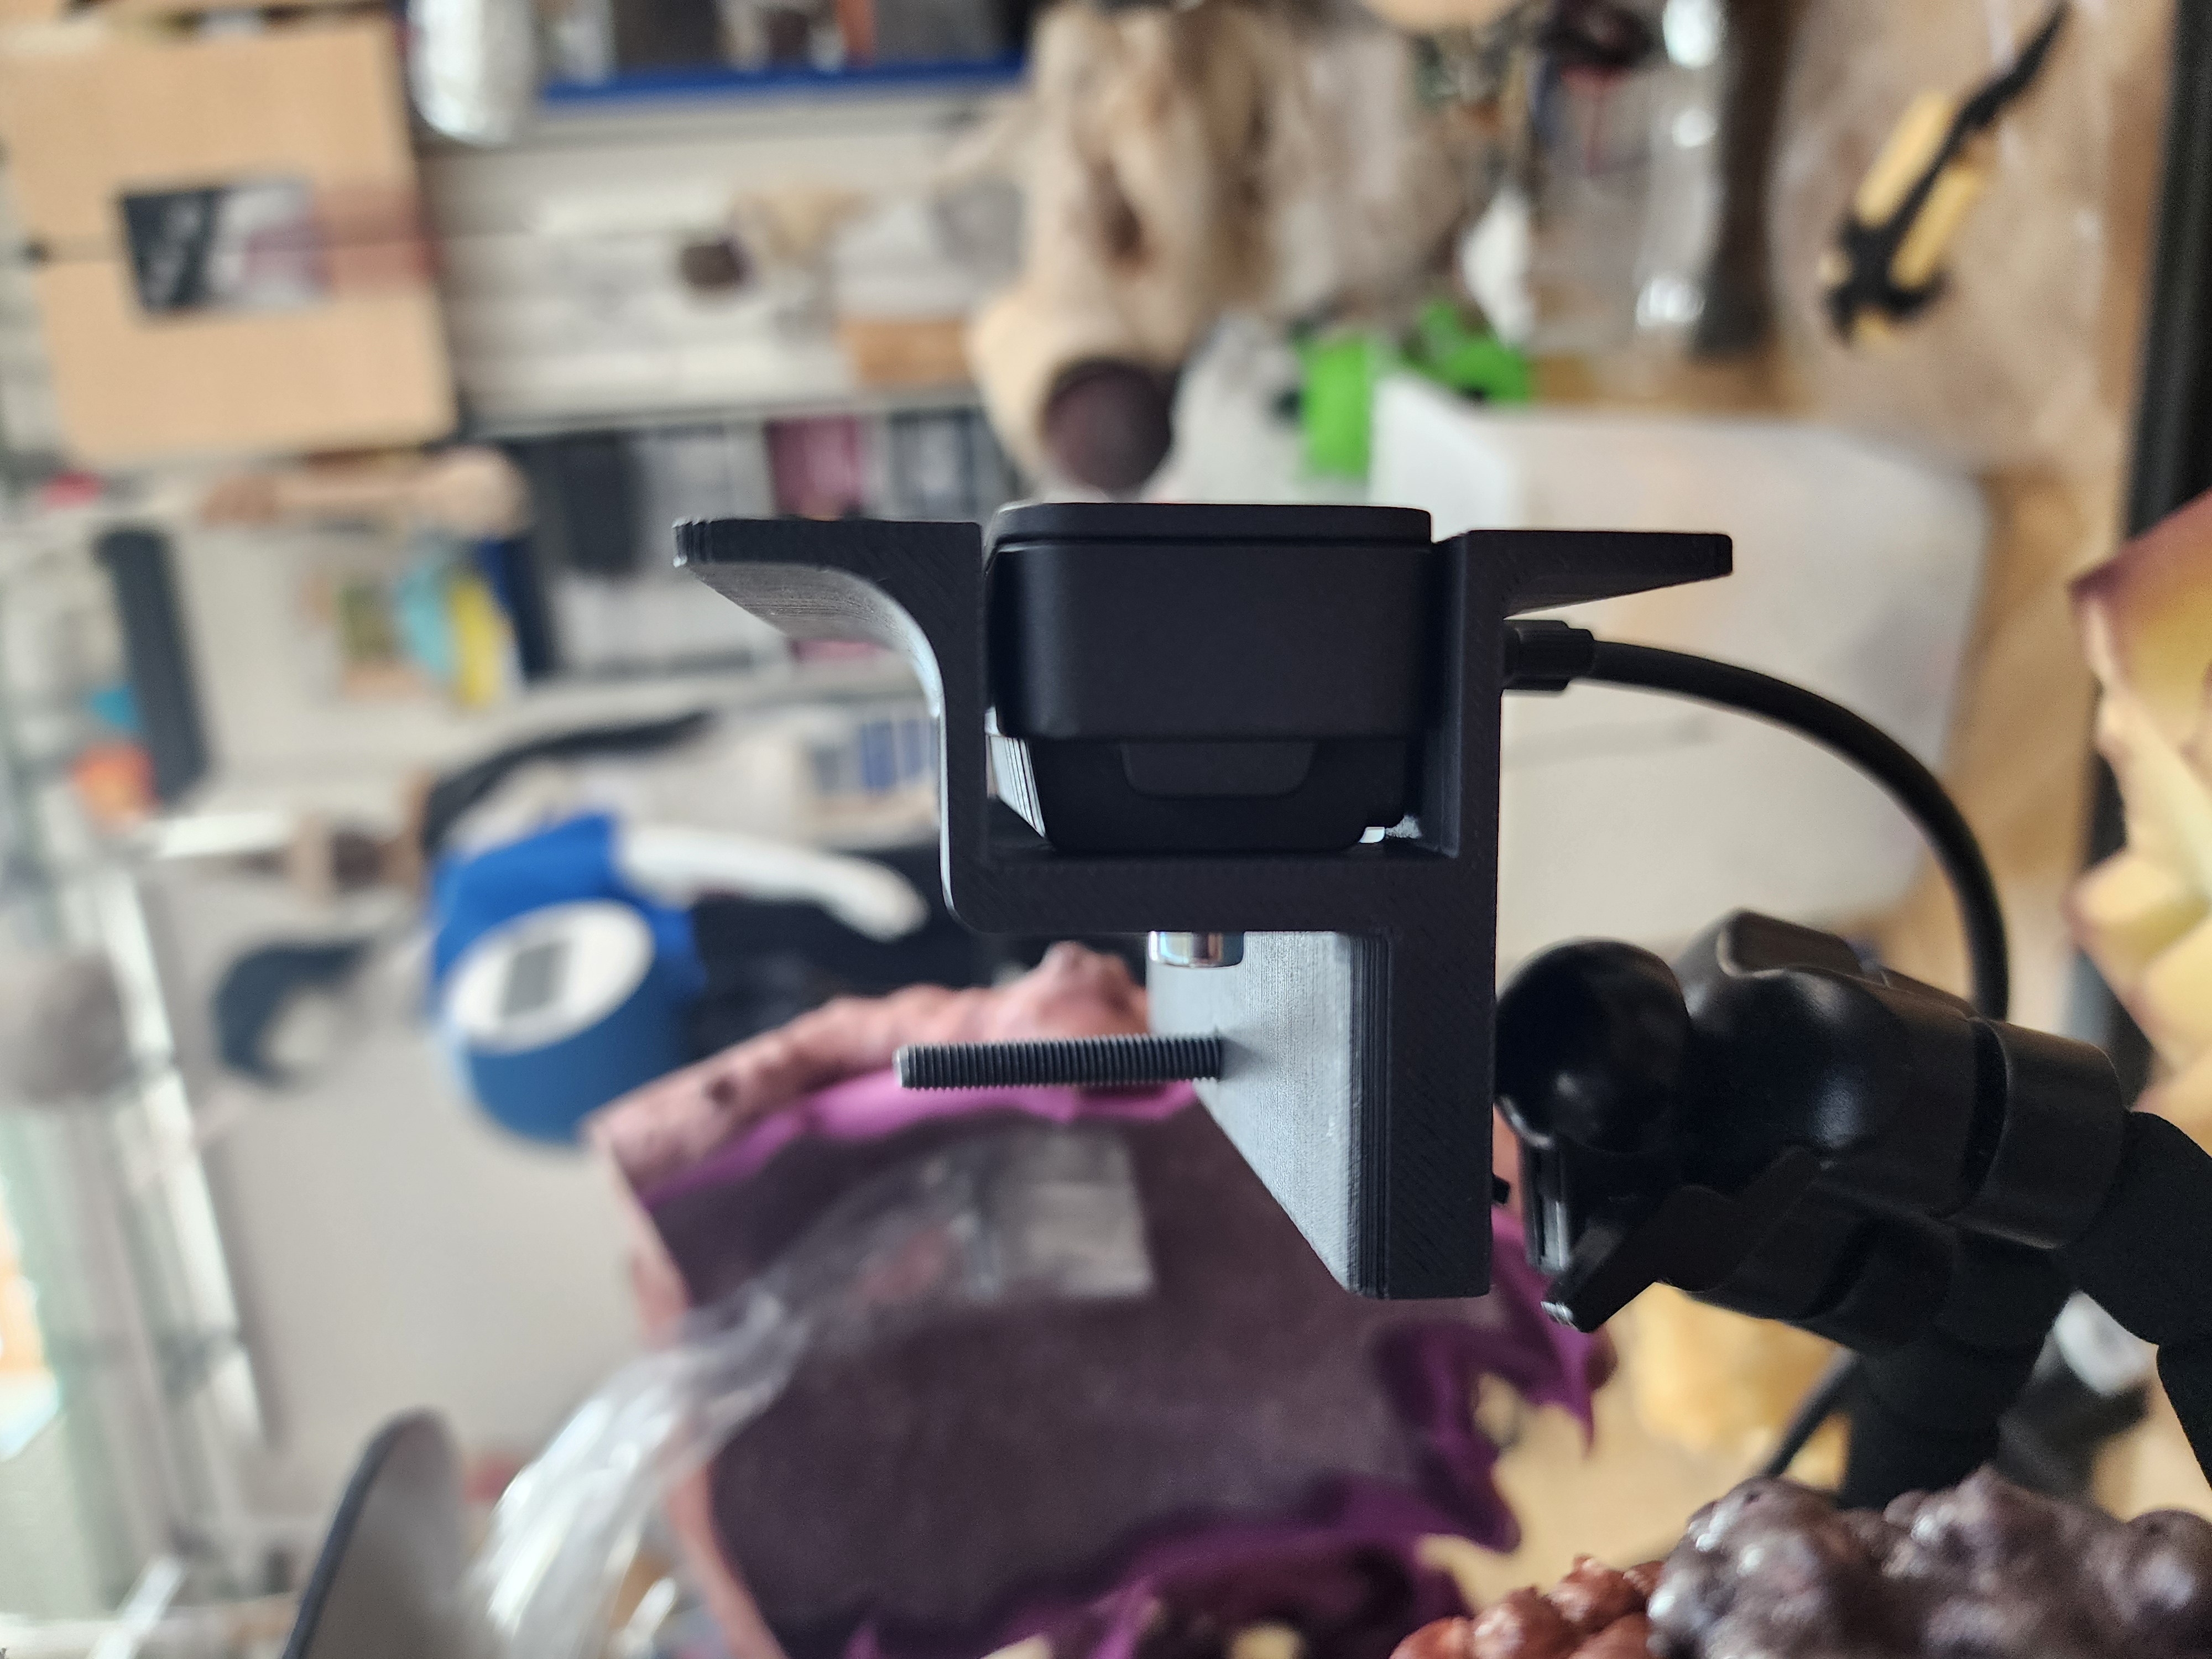
\includegraphics[width=\textwidth, angle=-90]{Images/CameraCasingNoMesh (4).jpg}
        \caption{Camera Casing without Mesh Covering (Side View)}
        \label{fig:camera_casing_no_mesh_side}
    \end{minipage}
    \hfill
    \begin{minipage}{0.45\textwidth}
        \centering
        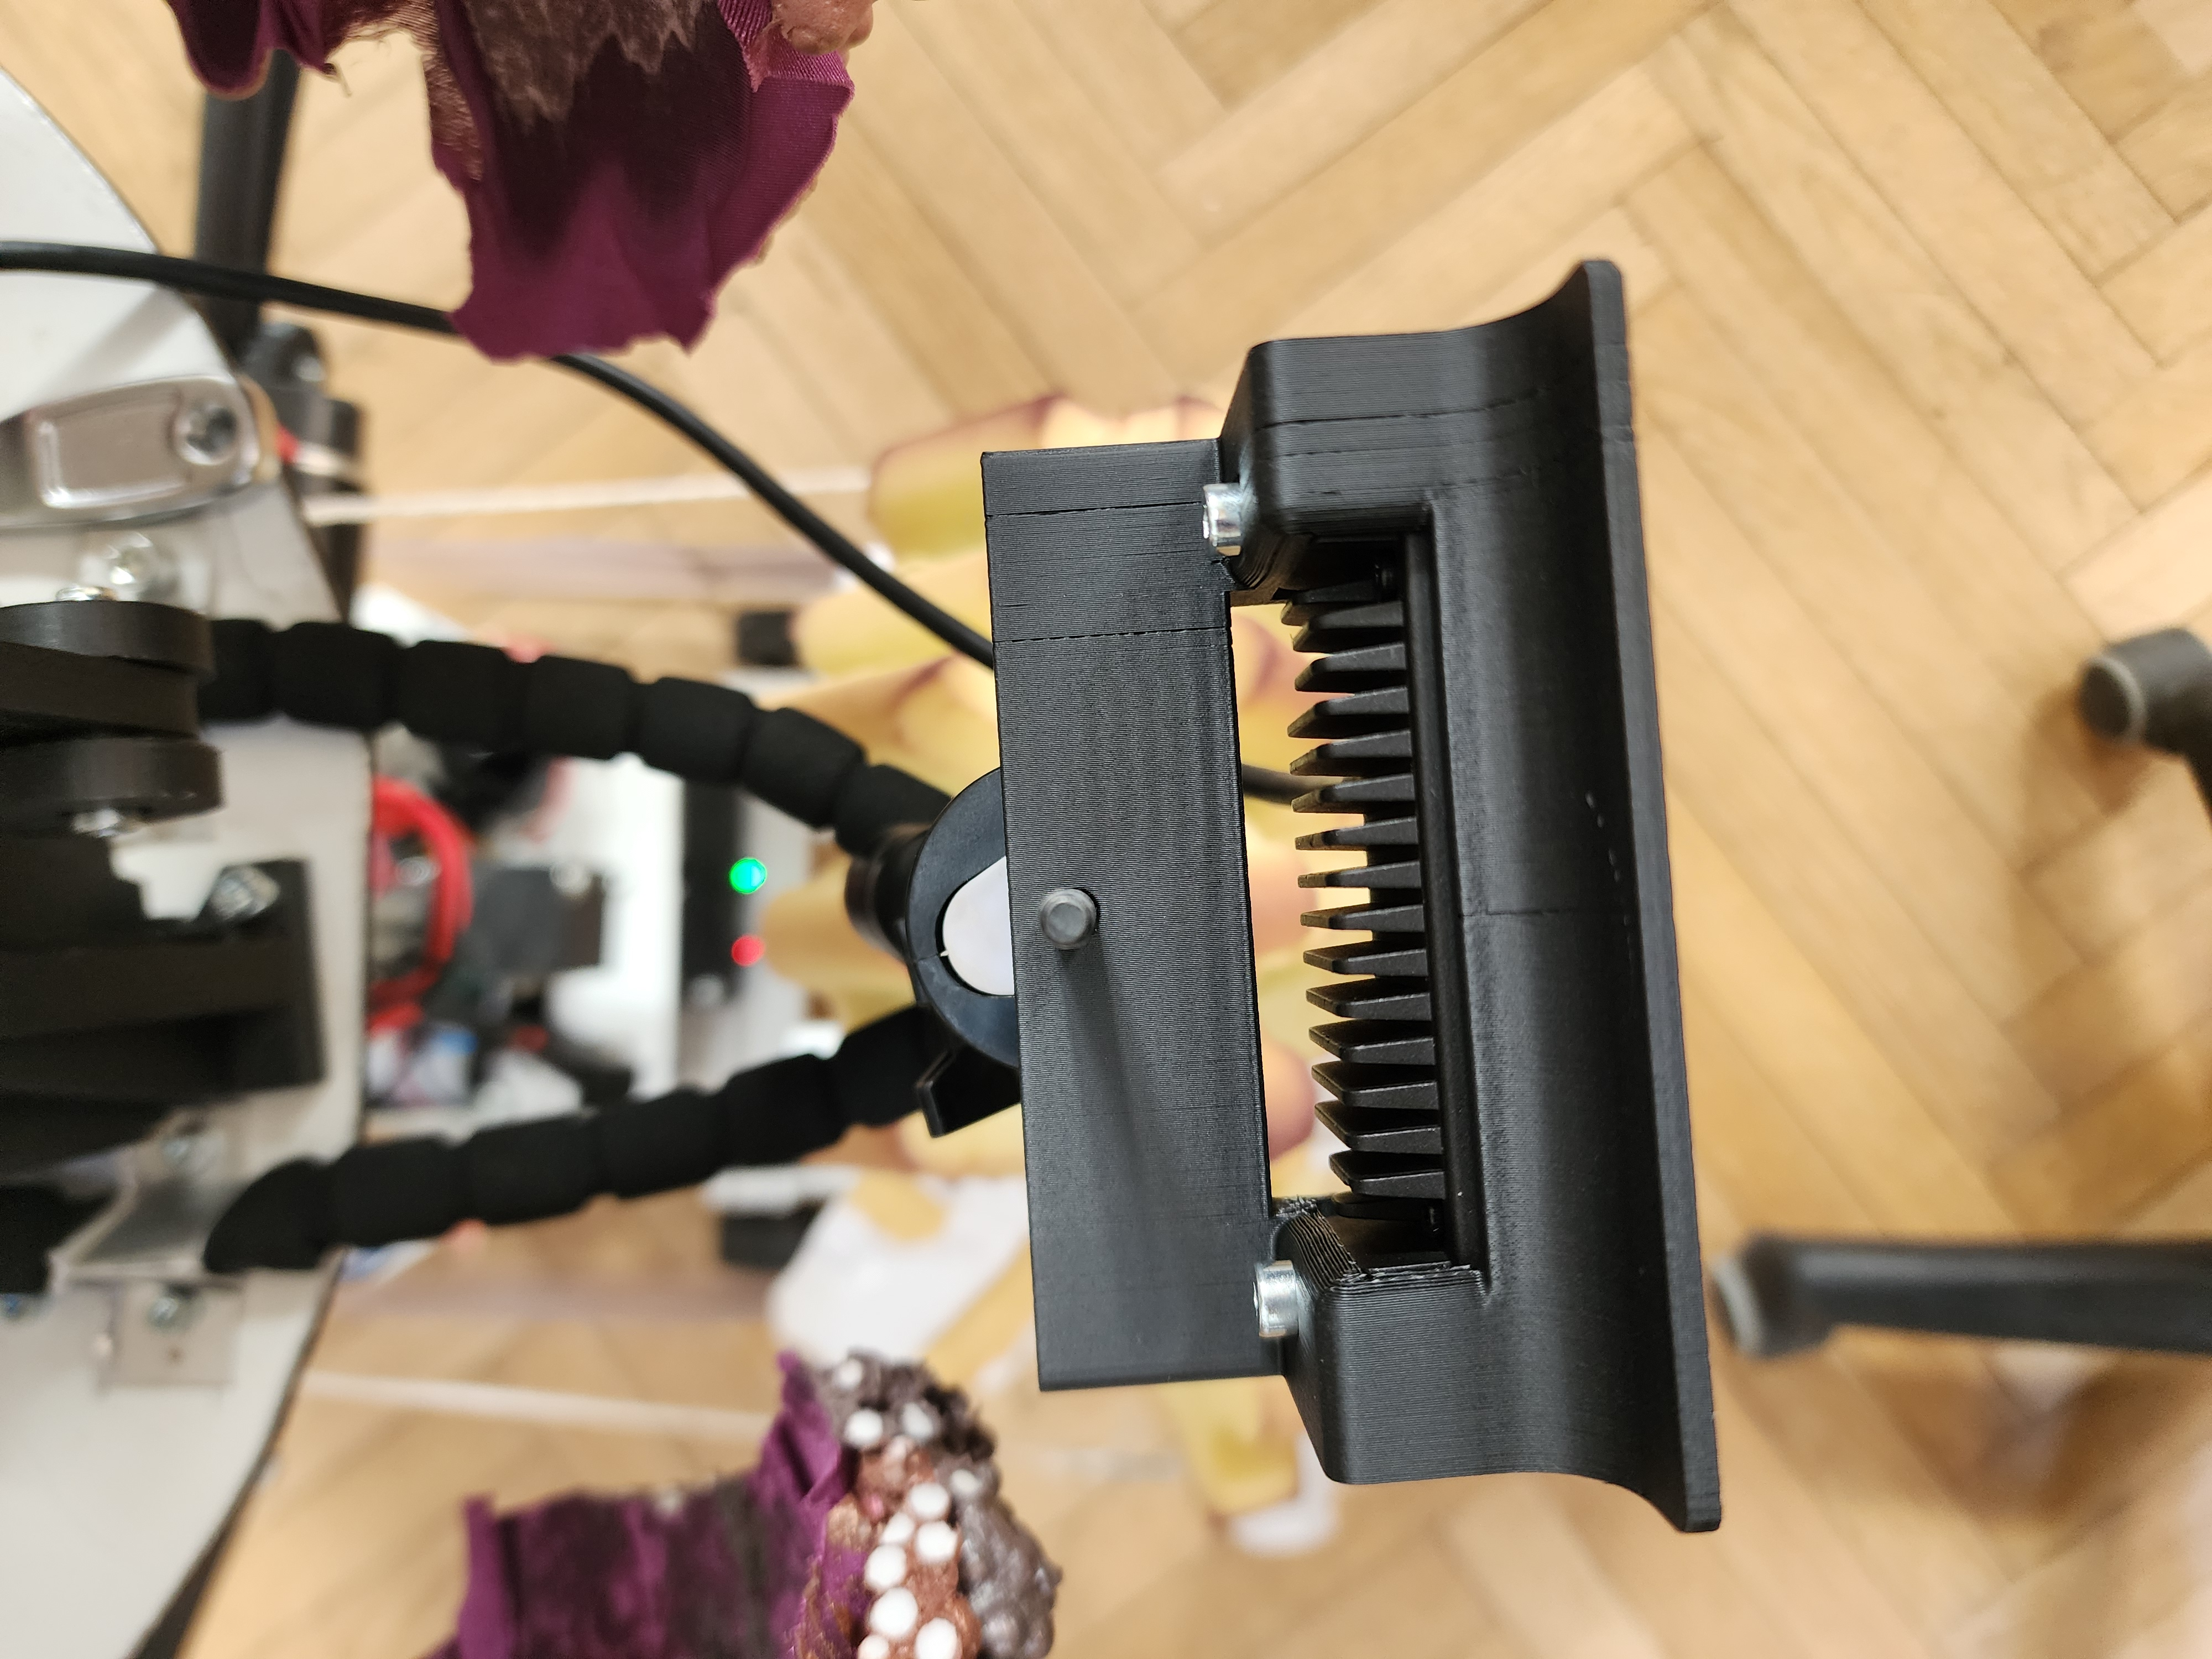
\includegraphics[width=\textwidth, angle=-90]{Images/CameraCasingNoMesh (3).jpg}
        \caption{Camera Casing without Mesh Covering (Top View)}
        \label{fig:camera_casing_no_mesh_top}
    \end{minipage}
\end{figure}

Field testing validates velcro system effectiveness during extended operational periods including various robot movements and interaction scenarios, ensuring consistent camera performance throughout typical social interaction scenarios while maintaining minimal image quality degradation.

% REORG_TAG: moved here from Audio System Integration
\subsection{Audio System Integration}

The audio system integration enables comprehensive bidirectional communication capabilities for VR integration and enhanced human-robot interaction, addressing the need for high-quality audio capture and dynamic sound generation that supports Tino's social presence and character expression. The system required careful hardware selection and sophisticated software implementation to achieve seamless integration with Tino's existing systems while maintaining acoustic performance within the constrained head environment.

\subsubsection{Hardware Implementation and Acoustic Design}

The audio hardware selection prioritized high-quality bidirectional communication capability while maintaining integration compatibility with Tino's system architecture and space constraints. The iTalk-01 omnidirectional microphone provides 360-degree audio capture capability suitable for social robot interaction scenarios where human positioning varies continuously, with microphone positioning optimization balancing audio quality against mechanical protection and aesthetic integration requirements through strategic fabric modifications.

The speaker system selection prioritized clear audio reproduction within the geometric and weight constraints of Tino's head assembly, with speaker placement within the servo head maximizing available space utilization while providing optimal acoustic coupling. Integration with existing head systems ensures speaker mounting does not interfere with Stewart platform operation, camera mounting, or other head-mounted systems.

\subsubsection{Speaker Mounting System Implementation}

The speaker system implementation prioritizes clear audio reproduction while addressing the practical requirements of maintenance access and acoustic optimization within Tino's constrained head geometry. The mounting solution utilizes industrial-grade velcro strips to secure speakers within the servo head structure, providing a robust yet flexible attachment system that enables quick realignment and maintenance without requiring complete head disassembly.

The velcro mounting system addresses several critical design challenges inherent in social robot audio integration. Primary considerations include vibration isolation to prevent mechanical noise transmission to the head structure, precise positioning control for optimal acoustic coupling, and maintenance accessibility for speaker replacement or cable management. The hook-and-loop fastener approach provides sufficient holding force to maintain speaker position during normal operation while enabling tool-free removal for system maintenance.

Speaker positioning optimization balances acoustic performance against space utilization within the head assembly. The mounting location maximizes available internal volume while ensuring speaker drivers remain clear of the Stewart platform mechanism, camera mounting hardware, and power distribution systems. Strategic positioning enables optimal sound projection through the fabric head covering while maintaining the structural integrity required for head articulation operations.

The velcro implementation includes strategic placement of adhesive-backed hook strips on the internal head structure and corresponding loop strips attached to custom speaker brackets. This configuration distributes mounting forces across multiple contact points, reducing stress concentration that could lead to attachment failure during extended operation. The system accommodates thermal expansion differences between speaker components and head structure materials while maintaining consistent acoustic coupling.

Installation procedures ensure proper alignment verification through acoustic testing and mechanical clearance validation. The removable nature of the velcro system enables rapid speaker replacement in field conditions, supporting efficient maintenance workflows that minimize robot downtime. Cable management integration ensures speaker wires remain secured and protected during head movement operations while maintaining accessibility for troubleshooting.

\begin{figure}[H]
    \centering
    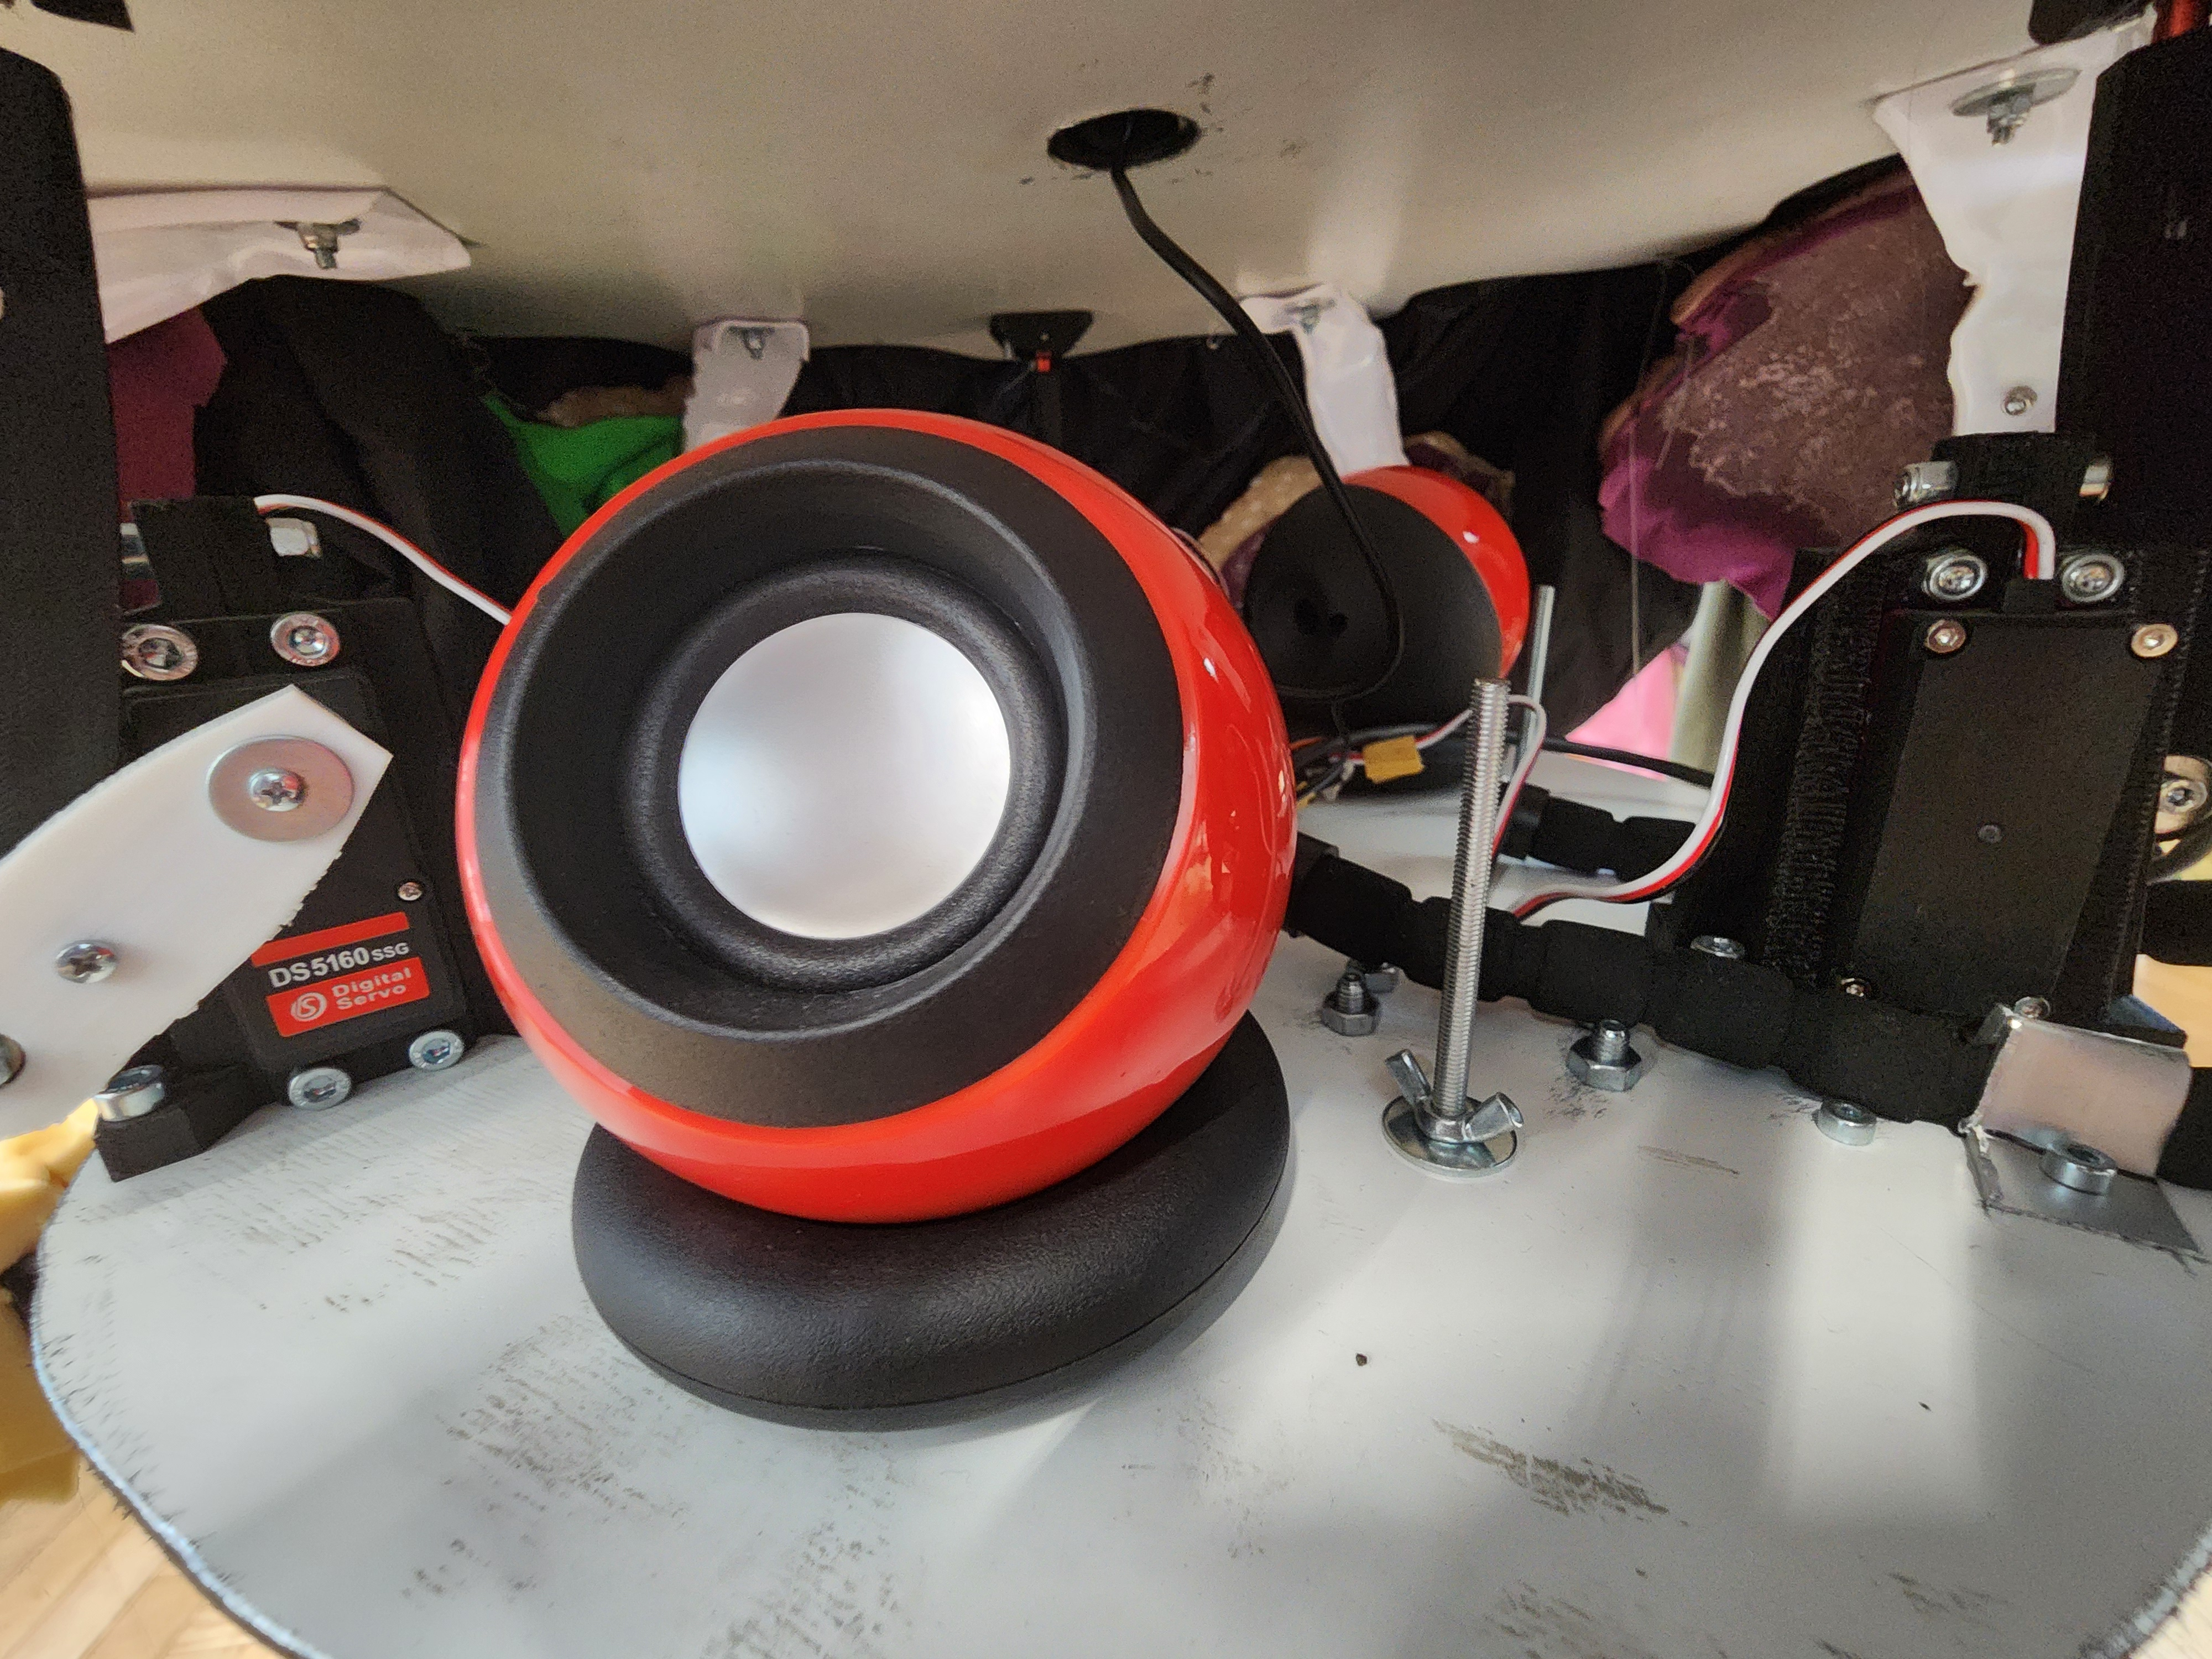
\includegraphics[height=6cm]{Images/SpeakerSetup (2).jpg}
    \caption{Speaker Mounted within Servo Head Structure}
    \label{fig:speaker_mount}
\end{figure}

\subsection{External Appearance Impact Assessment}

Throughout the comprehensive Tino V2 hardware implementation encompassing kinematic base redesign, power system overhaul, Stewart platform improvements, camera integration, and audio system enhancements, the robot's external aesthetic appearance has been deliberately preserved to maintain its distinctive character and proven social interaction capabilities.

The extensive internal modernization—from the fundamental shift to differential drive kinematics and enhanced power distribution to the complete redesign of head mechanisms and sensor integration—was strategically executed to operate within Tino's established external form factor. Each hardware upgrade was carefully engineered to enhance technical capabilities while preserving the approachable aesthetic that defines Tino's social robotics effectiveness. The fabric integration system, camera concealment mechanisms, and audio hardware placement all prioritize maintaining the robot's visual identity while enabling advanced functionality.

\begin{figure}[H]
    \centering
    \begin{minipage}{0.45\textwidth}
        \centering
        \includegraphics[width=\textwidth, angle=-90]{Images/TinoBefore.jpg}
        \caption{Tino Before V2 Implementation}
        \label{fig:tino_before_upgrade}
    \end{minipage}
    \hfill
    \begin{minipage}{0.45\textwidth}
        \centering
        \includegraphics[width=\textwidth, angle=-90]{Images/FinalTino.jpg}
        \caption{Tino After Complete V2 Upgrade}
        \label{fig:tino_after_upgrade}
    \end{minipage}
\end{figure}

The preservation of Tino's external design language validates the holistic engineering approach that achieved dramatic internal technological advancement while maintaining the established visual identity essential for consistent human-robot interaction research. This balance between comprehensive technical modernization and aesthetic continuity ensures that the V2 platform delivers enhanced capabilities without compromising the social robotics research foundation established by the original design, enabling seamless transition to the upgraded system while maintaining research validity and experimental continuity.

The comprehensive hardware implementation detailed throughout this section establishes the foundational platform that enables Tino V2's advanced capabilities. The kinematic base redesign provides the mobility precision required for sophisticated navigation algorithms, while the enhanced power distribution system supports the computational demands of modern perception and control systems. The redesigned Stewart platform head mechanism enables the fine-grained articulation necessary for natural social interaction, and the integrated camera system provides the visual input essential for advanced human-robot interaction. Most critically, the meticulously engineered audio hardware foundation—from microphone positioning for optimal capture to the velcro-mounted speaker system for maintenance accessibility—enables the sophisticated dynamic audio generation and VR integration capabilities that define Tino's enhanced social presence. This hardware foundation directly enables the advanced ROS2 software architecture, real-time VR integration, and intelligent audio generation algorithms detailed in the following chapter, where hardware capabilities transform into sophisticated robot behaviors that push the boundaries of social robotics.




\section{Software Architecture}
\label{sec:software_arch}

This software backbone supports the perception modules presented in Section~\ref{sec:perception_sensing}.

% REORG_TAG: moved here from ROS2 Architecture Design and Implementation
\subsection{ROS2 System Design}

The legacy monolithic Python architecture running on Raspberry Pi created critical limitations for real-time robotics applications: unreliable inter-process communication, insufficient computational parallelization, and poor scalability for advanced perception tasks. These constraints prevented effective utilization of modern multi-core processors and hindered integration of computationally intensive algorithms such as SLAM and human pose detection.

The migration to ROS2 framework addresses these fundamental limitations through its Data Distribution Service (DDS) middleware, which provides robust inter-process communication with Quality of Service guarantees for reliable data transmission under high computational loads. The distributed architecture enables optimal utilization of the NVIDIA Orin Nano's multi-core ARM Cortex-A78AE CPU and integrated GPU, allowing critical processes like SLAM computation, human pose detection, and sensor fusion to execute in parallel without blocking the main control loop. The standardized message interfaces and automatic discovery mechanisms facilitate seamless integration of new sensors while ensuring deterministic message delivery for time-critical operations.

This architectural foundation enables sophisticated multi-node processing capabilities that support real-time VR interaction, advanced perception algorithms, and reliable hardware control—capabilities that form the basis for the specialized node structure detailed in the following subsection.

\subsubsection{Tino's Physical Architecture}

Before examining the software node structure, it is essential to understand Tino's physical composition to provide context for the control systems described throughout this section. Tino is a mobile social robot designed with a distinctive non-anthropomorphic form that prioritizes expressive movement over human-like appearance.

The robot consists of four main physical components: a mobile \textbf{base} that provides differential drive locomotion using two powered wheels and a rear caster wheel (Figure~\ref{fig:tino_on_new_base}); a cylindrical \textbf{body} that houses the computational hardware (NVIDIA Orin Nano), power systems, and internal electronics while maintaining Tino's characteristic fabric-covered aesthetic; an articulated \textbf{head} mechanism that utilizes a three-degree-of-freedom Stewart platform configuration with servo motors to provide expressive pan, tilt, and pitch movements essential for social interaction (Figure~\ref{fig:head_arm_v2}); and a single-actuator \textbf{leg} mechanism that extends from the body to enable coordinated gestures synchronized with base movement.

\begin{figure}[H]
    \centering
    \begin{minipage}{0.3\textwidth}
        \centering
        \includegraphics[width=\textwidth]{Images/NewBaseDifferentialDrive.jpg}
        \caption{Differential Drive Base System}
        \label{fig:base_component}
    \end{minipage}
    \quad
    \begin{minipage}{0.3\textwidth}
        \centering
        \includegraphics[width=\textwidth]{Images/NewHeadDoubleJoint (2).jpg}
        \caption{Stewart Platform Head Mechanism}
        \label{fig:head_component}
    \end{minipage}
    \quad
    \begin{minipage}{0.3\textwidth}
        \centering
        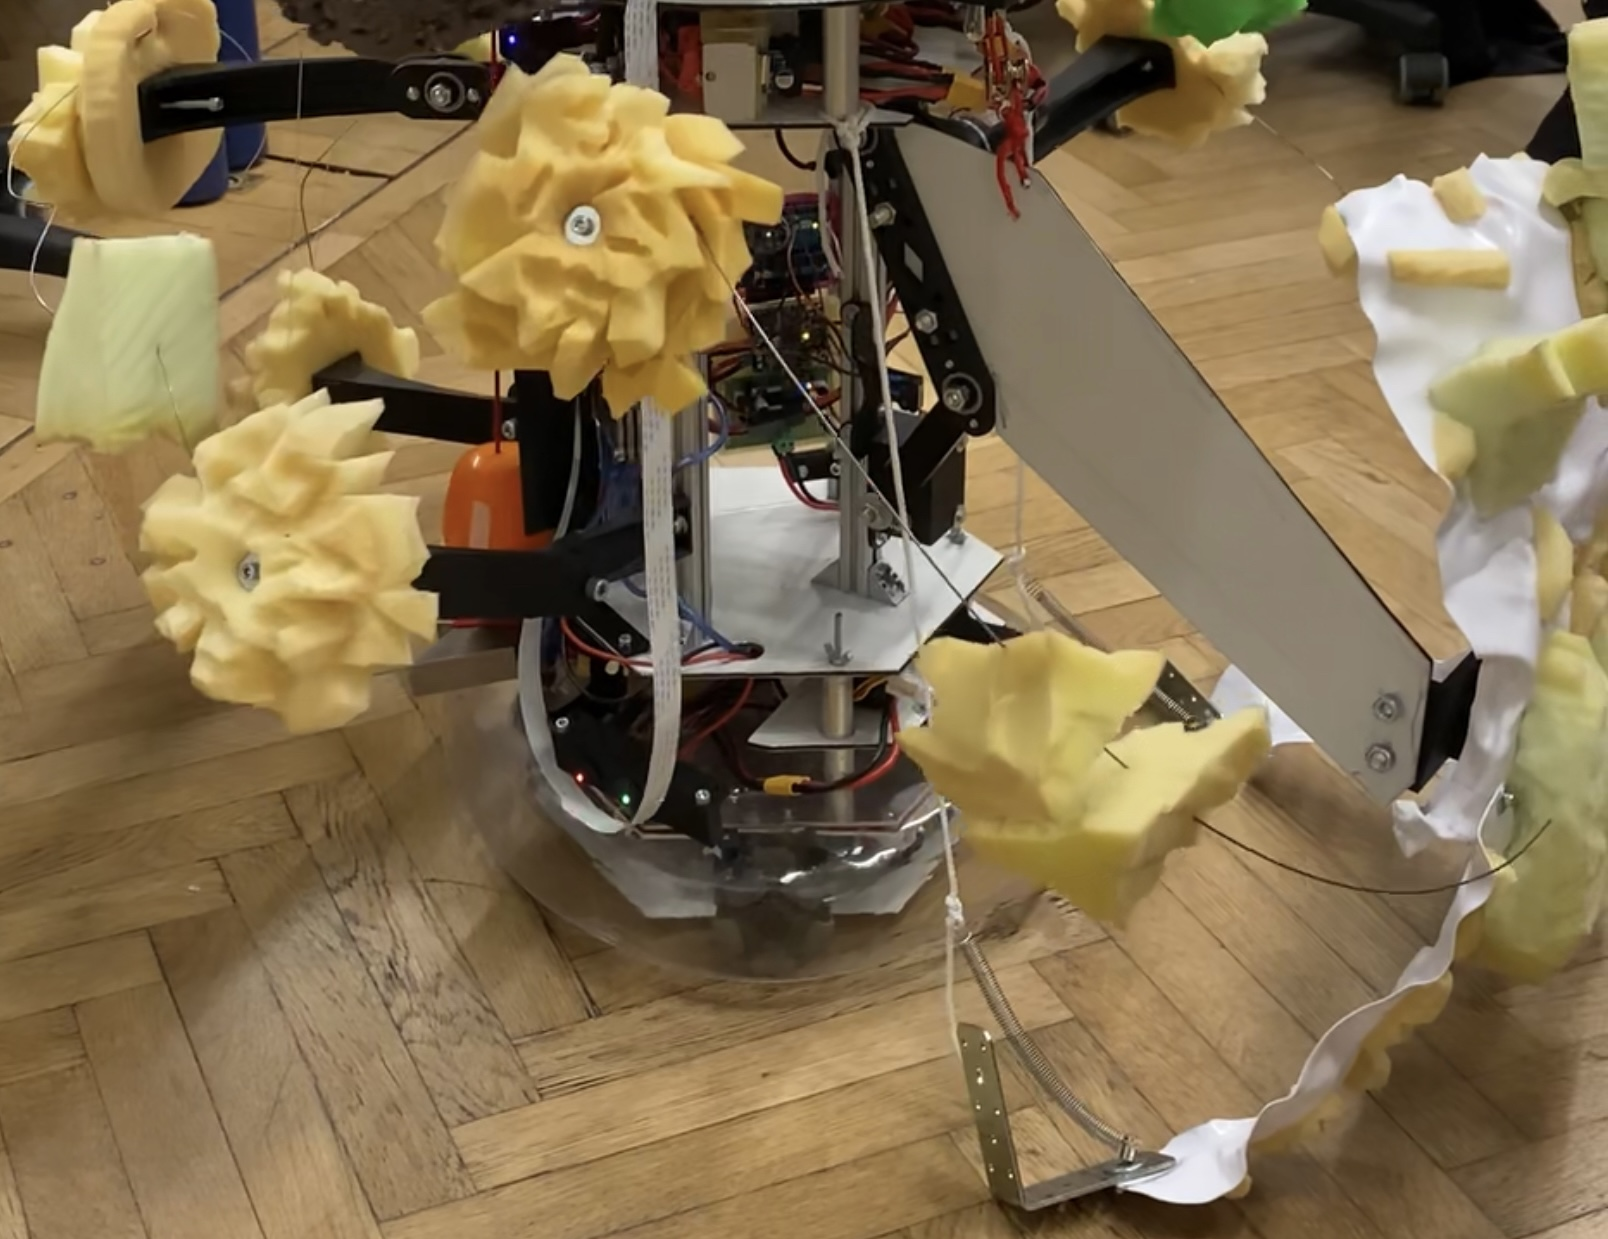
\includegraphics[width=\textwidth]{Images/leg_detail.jpg}
        \caption{Single-Actuator Leg Mechanism}
        \label{fig:leg_component}
    \end{minipage}
\end{figure}

This modular architecture enables each component to be controlled independently through dedicated Arduino microcontrollers while supporting coordinated behaviors essential for natural social interaction. The head platform provides fine-grained articulation for attention direction and social signaling, while the differential drive base ensures reliable mobility across various indoor environments. The leg mechanism enables expressive gestures that can be precisely coordinated with base movement to create natural locomotion patterns.

The complete robot assembly measures approximately 1.2 meters in height with the fabric head covering, creating an approachable scale for human interaction while housing sophisticated perception hardware including stereo cameras for SLAM and human detection capabilities. Figure~\ref{fig:tino_before_upgrade} and Figure~\ref{fig:tino_after_upgrade} in Section~\ref{sec:hardware_impl} illustrate Tino's external appearance before and after the V2 hardware upgrades, demonstrating how the enhanced internal capabilities were implemented while preserving the robot's distinctive social interaction aesthetic.

\subsubsection{Node Structure and Functionality}

Complex robotics systems require specialized subsystem management to handle diverse hardware interfaces, real-time perception processing, and external system integration without creating bottlenecks or single points of failure. The Tino V2 architecture addresses this through six specialized ROS2 nodes, each responsible for specific functionality while maintaining loose coupling through standardized message interfaces. The perception-focused nodes (Robot Controller for SLAM integration and Pose Detection for human tracking) are described here in terms of their architectural role, with detailed implementation specifics covered in Section~\ref{sec:perception_sensing}.

\paragraph{Gamepad Control Node}

Development and testing of robotic systems requires reliable manual control interfaces that can replicate VR command patterns for validation purposes. The \texttt{gamepad\_node.py} addresses D-input to X-input compatibility issues on Linux while implementing pulse generation mechanisms that replace continuous joystick input with discrete 3-cycle command pulses (120ms duration at 25Hz). Button mapping follows VR command structure: face buttons control leg states (X=1, Y=2, B=3, A=0) and bumpers trigger rotation commands. This node enables comprehensive testing of robot behaviors without VR hardware dependency, ensuring system reliability during development phases. A more detailed analysis of the underlying control architecture and the complete pulse-based command system that enables this seamless VR-gamepad compatibility will be examined in Section~\ref{sec:control_implementation}.

\begin{figure}[H]
    \centering
    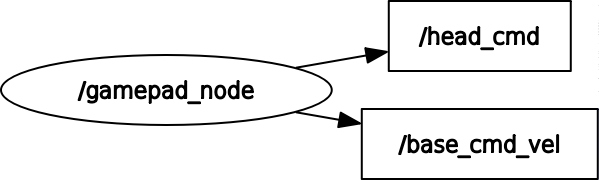
\includegraphics[width=0.8\textwidth]{Images/gamepadnode.png}
    \caption{RQT Graph visualization of the Gamepad Control Node showing topic connections and data flow patterns.}
    \label{fig:rqt_gamepad_node}
\end{figure}

\paragraph{Hardware Interface Node}

Multiple Arduino subsystems with individual serial interfaces create device identification and communication coordination challenges that require robust connection management. The \texttt{hardware\_interface\_node.py} manages parallel serial communication with three Arduino subsystems through persistent device symlinks (\texttt{/dev/ttyBASE}, \texttt{/dev/ttyLEG}, \texttt{/dev/ttyHEAD}) created via udev rules. Each thread operates at 115200 baud with configurable message repetition and command format \texttt{BF:value\_BB:value\_HP:value\_HX:value\_HY:value}. Automatic device discovery, connection monitoring, and graceful degradation enable reliable hardware control even when individual subsystems become unavailable, providing the foundation for coordinated movement execution.

\begin{figure}[H]
    \centering
    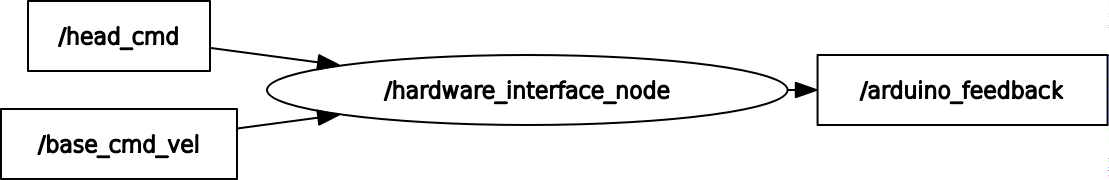
\includegraphics[width=0.8\textwidth]{Images/hardwarenode.png}
    \caption{RQT Graph visualization of the Hardware Interface Node showing topic subscriptions and Arduino communication patterns.}
    \label{fig:rqt_hardware_interface_node}
\end{figure}

\paragraph{Robot Controller Node}

Advanced robotics systems require centralized coordination to manage sensor fusion, localization monitoring, and behavior orchestration while preventing conflicts between subsystems. The \texttt{robot\_controller\_node.py} implements sophisticated localization supervision including RTAB-Map orientation loss detection (quaternion: x=1.0, y=0.0, z=0.0, w=0.0), automatic odometry reset via \texttt{/reset\_odom} service, and orientation estimation from movement history when RTAB-Map becomes unreliable. Sensor fusion combines UWB absolute positioning with RTAB-Map orientation data, applying 11.5-degree rotation correction to align coordinate frames, then publishes unified pose data to \texttt{/vr\_in/robot\_pose}. This central coordination enables reliable localization and seamless communication with VR systems while providing comprehensive system health monitoring.

\begin{figure}[H]
    \centering
    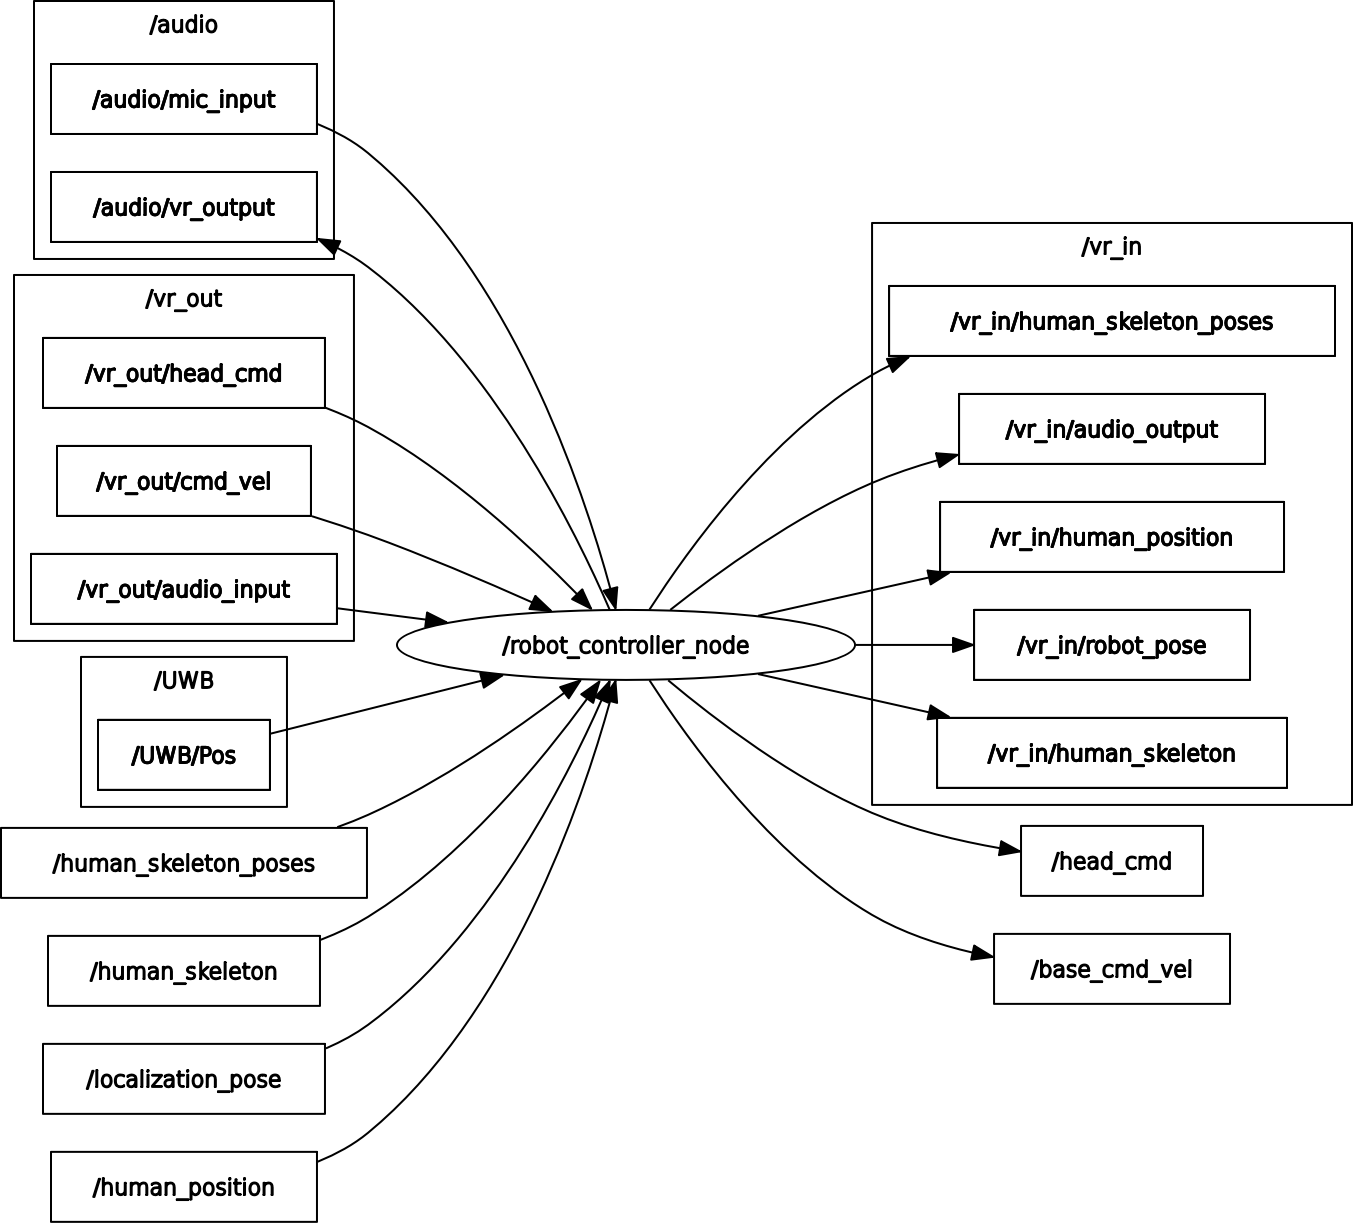
\includegraphics[width=0.8\textwidth]{Images/robotcontrollernode.png}
    \caption{RQT Graph visualization of the Robot Controller Node showing sensor fusion topic connections and VR pose data publication.}
    \label{fig:rqt_robot_controller_node}
\end{figure}

\paragraph{Pose Detection Node}

Real-time human interaction requires robust detection and tracking capabilities that can provide accurate 3D positioning for VR integration and social robotics research. The \texttt{pose\_detection\_node.py} implements YOLOv11 optimized with TensorRT for Orin Nano performance, combining 2D pose estimation with stereo depth information from Oak-D Pro cameras (\texttt{/right/image\_rect}, \texttt{/stereo/depth}). The system publishes detection results to multiple topics: human position data (\texttt{/human\_position}), visualization markers (\texttt{/human\_skeleton}), and structured pose arrays (\texttt{/human\_skeleton\_poses}) with exactly 17 COCO-format joints. Closest-person selection algorithms and temporal smoothing ensure consistent 3D positioning across varying distances, enabling precise human tracking for VR interaction scenarios.

\begin{figure}[H]
    \centering
    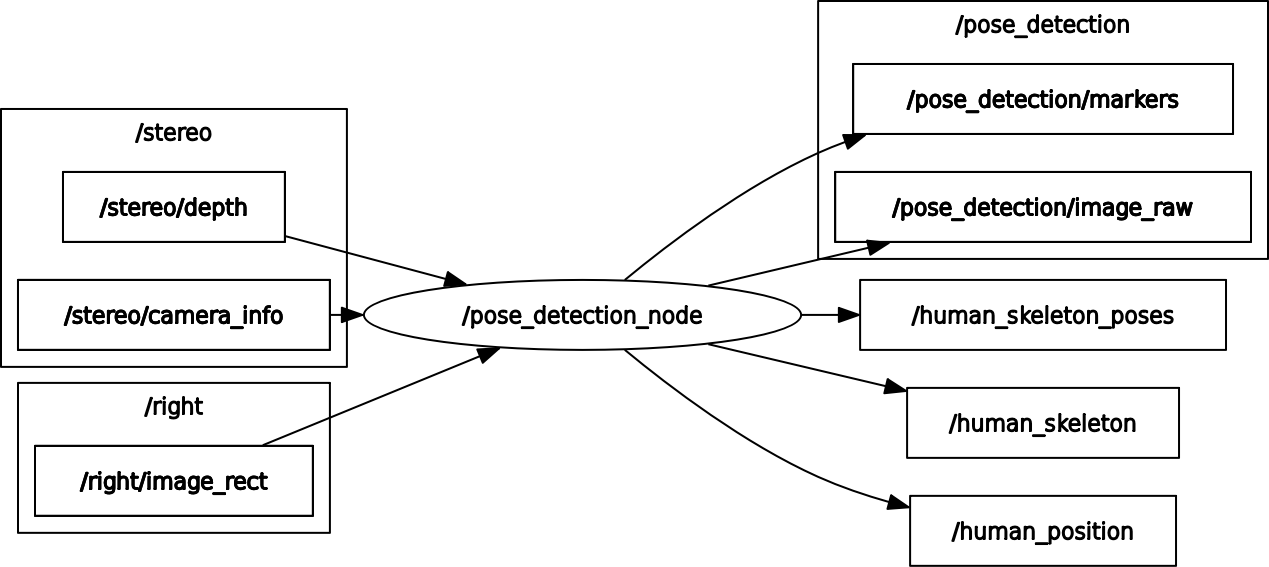
\includegraphics[width=0.8\textwidth]{Images/posenode.png}
    \caption{RQT Graph visualization of the Pose Detection Node showing stereo camera topic subscriptions and human tracking data publication.}
    \label{fig:rqt_pose_detection_node}
\end{figure}

\paragraph{VR Integration Node}

VR system integration requires comprehensive bidirectional communication between Unity VR environments and robot systems, addressing challenges in real-time responsiveness, spatial coordination, and user experience consistency while supporting audio feedback capabilities. The \texttt{vr\_interface\_node.py} implements a sophisticated multi-threaded architecture that consolidates all VR communication through custom UDP protocols optimized for ultra-low latency and deterministic message delivery.

The three-port UDP architecture isolates data streams to prevent interference: port 5005 handles incoming 32-byte VR command packets at expected 25Hz rate, port 5006 transmits 24-byte robot pose data at 10Hz, and port 5007 streams 208-byte skeleton data at 10Hz. This isolation enables independent optimization for different latency requirements while supporting flexible deployment through configurable IP addresses (default 192.168.0.201). Traditional ROS2 bridge solutions introduce excessive overhead for real-time VR scenarios, necessitating this custom protocol optimized for robot-VR interaction patterns.

Incoming VR commands utilize binary format with \texttt{struct.unpack('fffiiffi', data)} containing head control floats (pitch/pan/tilt), base command integers (state 0--3, angular direction --1/0/1), and audio parameters (volume 0--255, orientation --1.0 to 1.0) with message ordering validation. The node processes these commands through dedicated listener threads with 1-second timeouts and publishes corresponding movement commands to \texttt{/vr\_out/cmd\_vel} and \texttt{/vr\_out/head\_cmd} topics.

Outgoing data transmission provides continuous robot state information through 24-byte pose packets (position coordinates, orientation quaternion, audio volume) and 208-byte skeleton data containing exactly 17 COCO-format joints with default (0,0,0) coordinates for missing joints. Audio integration enables bidirectional communication where the node receives audio output from \texttt{/vr\_in/audio\_output} topics and processes VR audio control parameters including volume control (0--255) and spatial orientation (--1.0 to 1.0) for real-time audio modification based on VR user interaction and spatial positioning.

The audio control system utilizes ROS2 topics to enable dynamic audio modification based on VR user interaction and robot state. Volume control implementation applies logarithmic scaling to provide natural perceived loudness variations, while orientation-based parameter modulation enables frequency shifting and audio characteristic changes based on spatial positioning, creating spatial audio awareness that enhances immersive VR interaction. The stereo speaker system provides sophisticated spatial audio through quadratic intensity scaling with exponential panning response, creating pronounced left-right separation that follows VR user head movements without audible artifacts.

Communication health monitoring implements comprehensive reliability features including message rate validation against configured targets, connection status tracking with 3-second disconnection timeout, message ordering validation for duplicate/loss detection, and automatic recovery with counter reset upon reconnection. This robust foundation enables immersive robot control through natural VR gestures while providing comprehensive environmental awareness and responsive audio feedback that enhances social presence and interaction naturalness.

\begin{figure}[H]
    \centering
    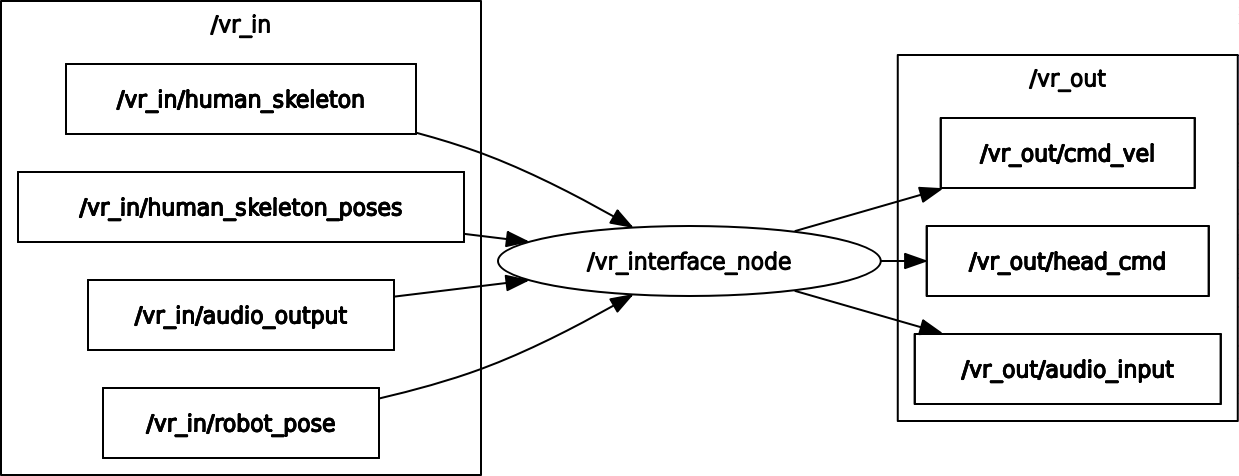
\includegraphics[width=0.8\textwidth]{Images/vrnode.png}
    \caption{RQT Graph visualization of the VR Interface Node showing bidirectional topic connections for VR communication and data exchange.}
    \label{fig:rqt_vr_interface_node}
\end{figure}

\subsubsection{Communication Protocols and Message Design}

Distributed robotics systems require reliable message exchange mechanisms that can handle diverse data types, latency requirements, and failure scenarios without compromising system performance. The ROS2 communication infrastructure implements a topic-based publish-subscribe architecture with Quality of Service policies optimized for robot pose data (reliable delivery, history depth 10), real-time human tracking (best-effort for continuous streams), and critical movement commands (reliable delivery with immediate processing).

The message hierarchy follows logical data flow patterns: VR input topics (\texttt{/vr\_out/cmd\_vel}, \texttt{/vr\_out/head\_cmd}) carry external commands, internal processing topics (\texttt{base\_cmd\_vel}, \texttt{head\_cmd}) handle robot control, and output topics (\texttt{/vr\_in/robot\_pose}, \texttt{/vr\_in/human\_position}) provide data to external systems. Robot pose utilizes \texttt{geometry\_msgs/PoseStamped} with high-precision timestamps for sensor fusion, while human detection employs \texttt{geometry\_msgs/PoseArray} containing exactly 17 COCO-format joints with consistent 3D coordinates. VR commands leverage \texttt{geometry\_msgs/Twist} where \texttt{linear.x} carries leg states (0--3) and \texttt{angular.z} carries rotation commands (--1, 0, 1).

Synchronous operations utilize ROS2 service calls, particularly the \texttt{/reset\_odom} service (\texttt{std\_srvs/Empty}) for RTAB-Map odometry reset when orientation loss is detected. This communication foundation provides the infrastructure necessary for sophisticated audio generation systems that enhance robot personality and social interaction capabilities, as detailed in the following subsection.

\begin{figure}[H]
    \centering
    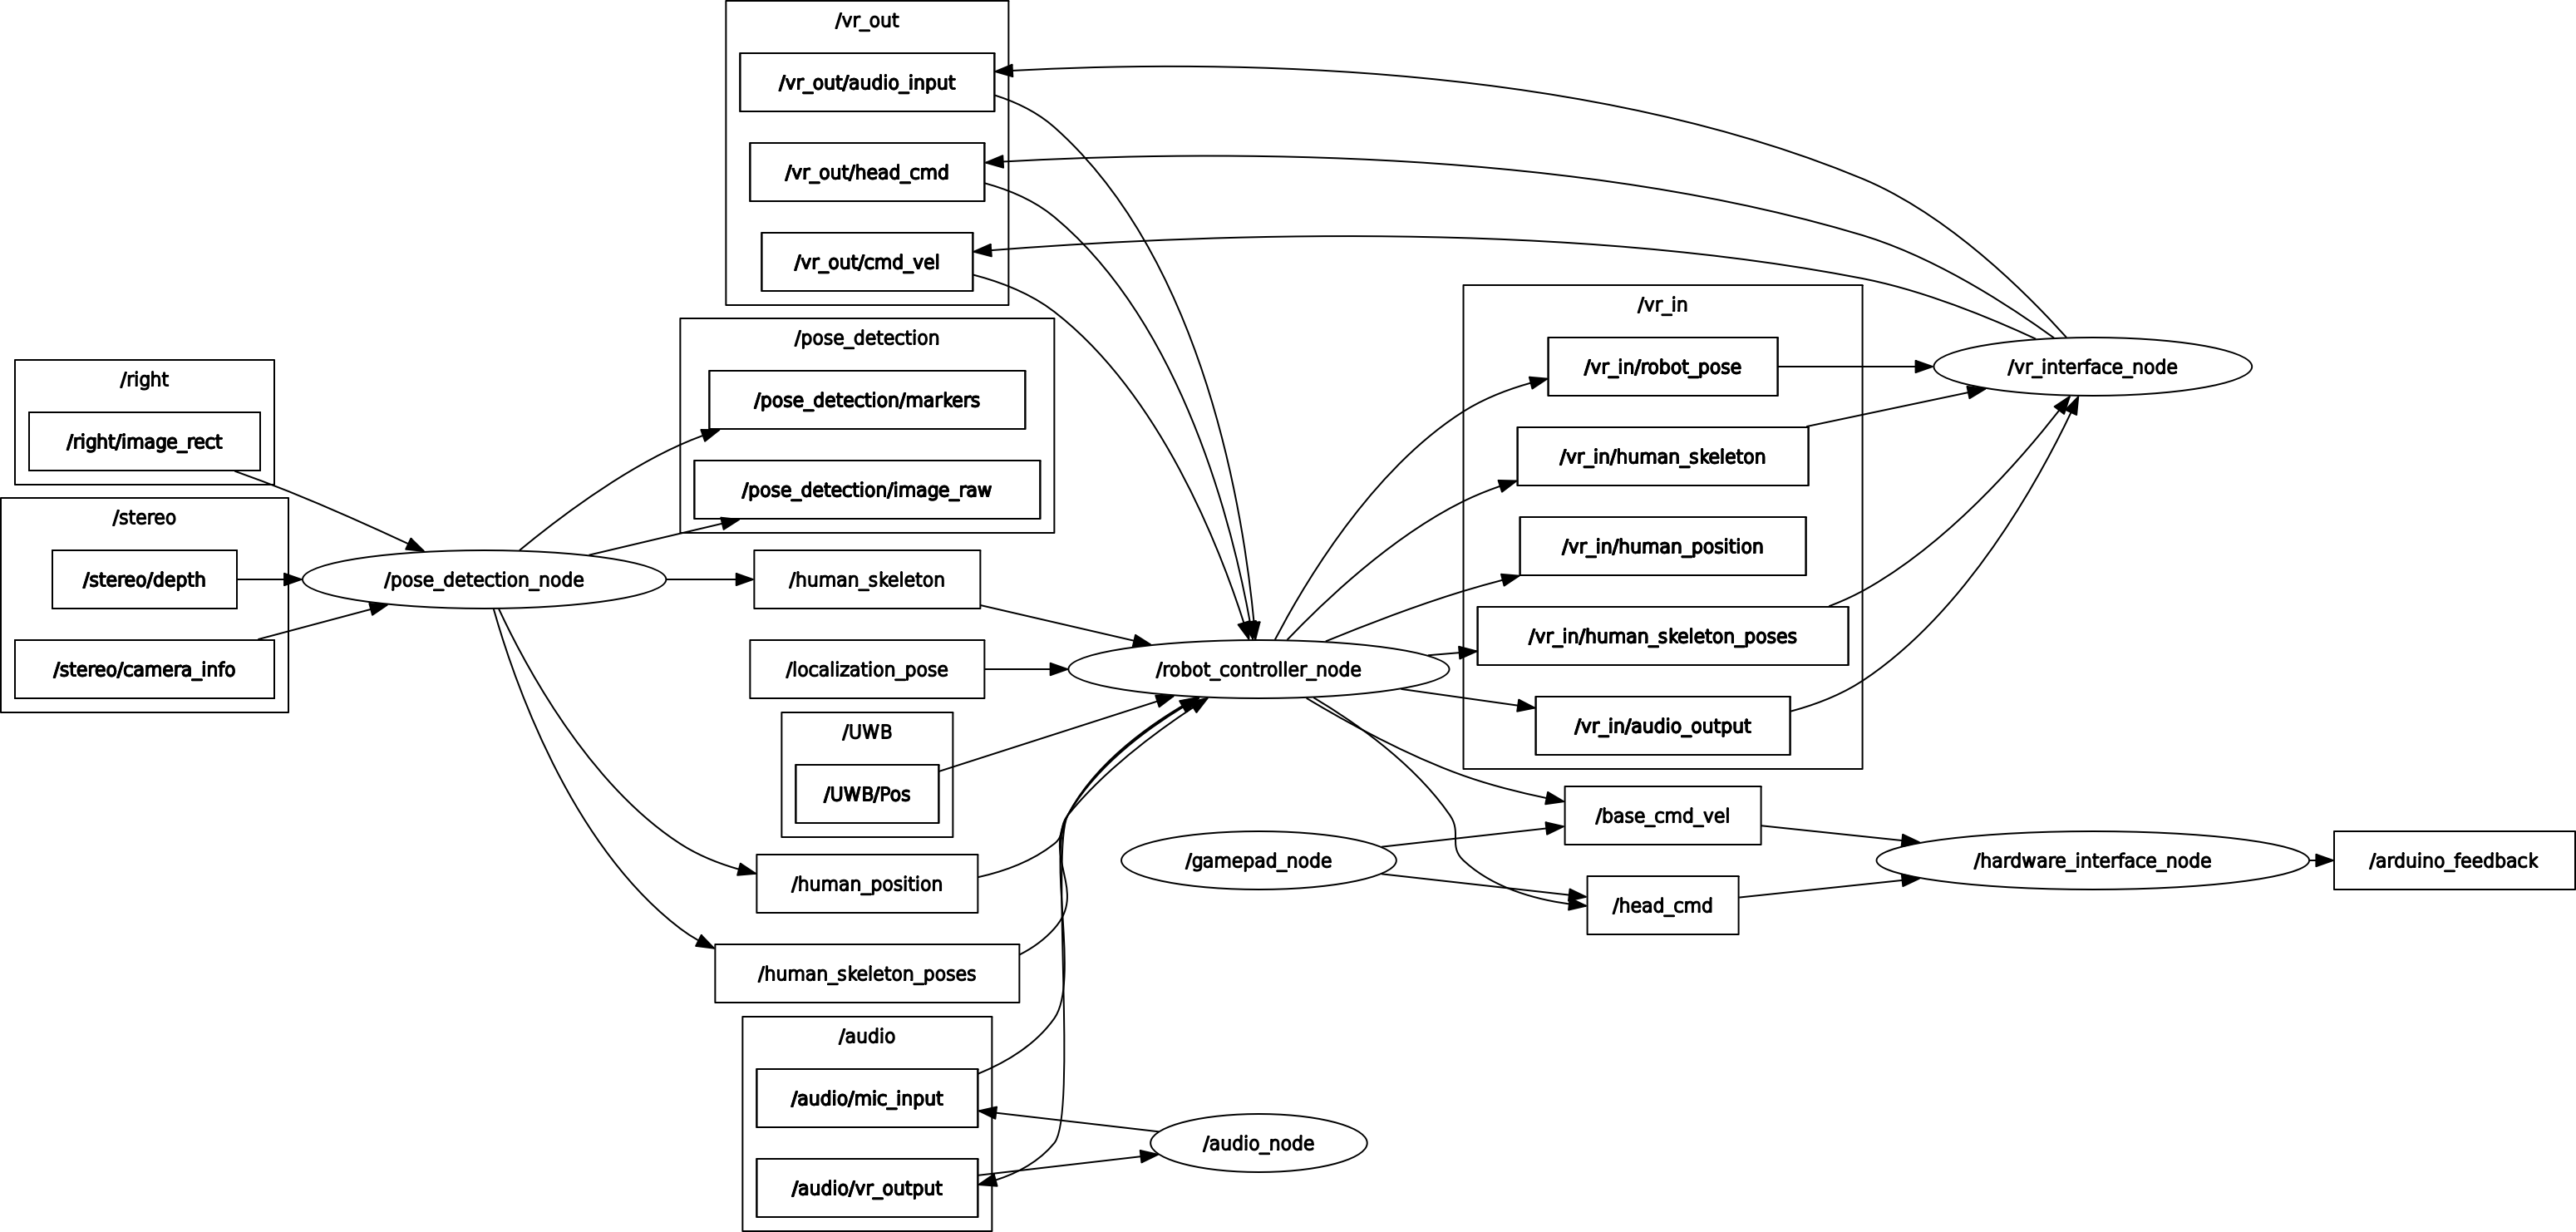
\includegraphics[width=\textwidth]{Images/fulltinonodes.png}
    \caption{Complete RQT Graph visualization showing all Tino V2 ROS2 nodes operating simultaneously, illustrating the comprehensive communication architecture with all topic connections, service calls, and data flow patterns across the entire robotic system.}
    \label{fig:rqt_complete_system}
\end{figure}

\begin{figure}[H]
    \centering
    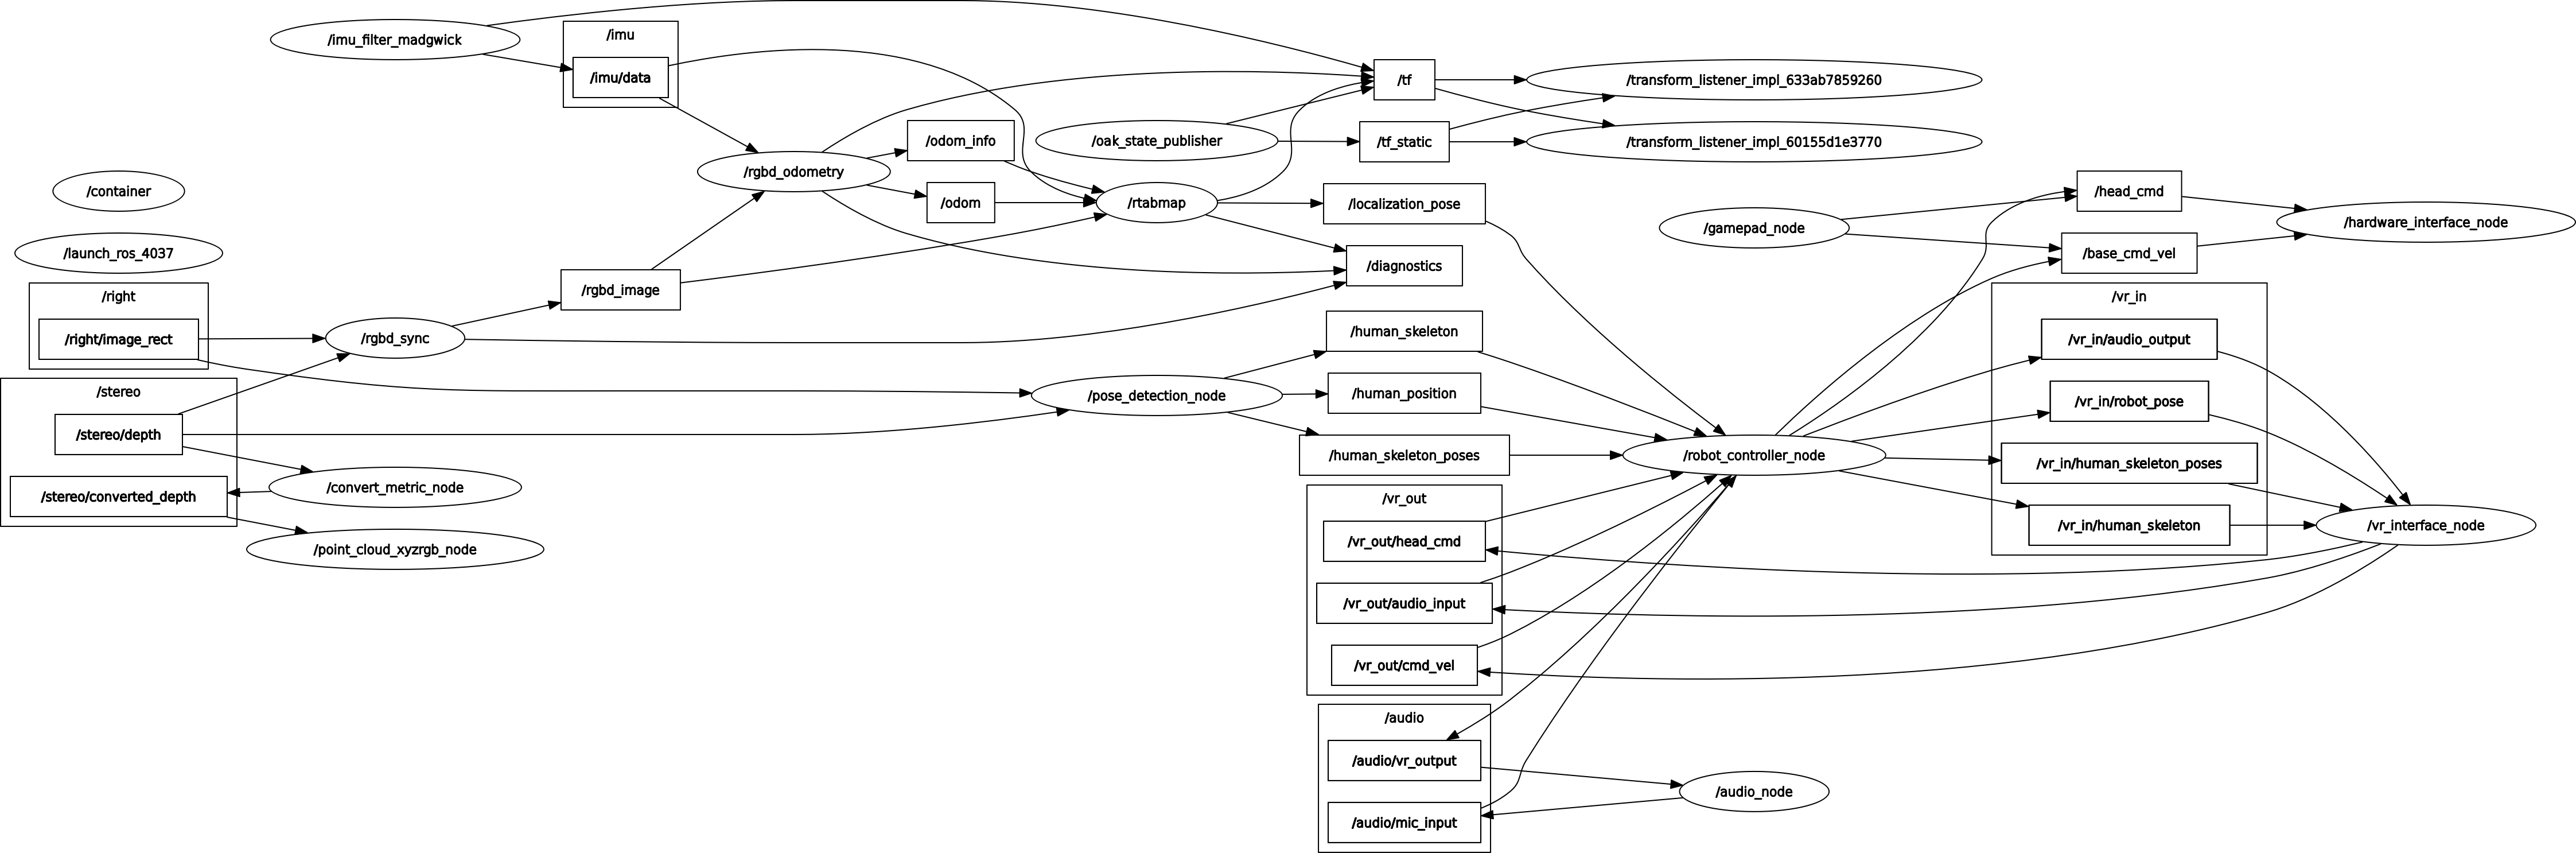
\includegraphics[width=\textwidth]{Images/TinoWithRTAB.png}
    \caption{Comprehensive RQT Graph visualization including RTAB-Map SLAM system and stereo camera nodes alongside all Tino V2 custom nodes. Note: Due to the extensive number of nodes and interconnections in the complete perception pipeline, this visualization may appear complex and dense, but demonstrates the full operational scope of the integrated robotic system.}
    \label{fig:rqt_complete_system_with_rtab}
\end{figure}

\subsection{Dynamic Audio Generation}

Social robotics research requires expressive audio capabilities that enhance robot personality and enable emotional communication beyond visual cues. Traditional robotic audio systems use pre-recorded sounds or basic text-to-speech, limiting the range of emotional expression and adaptability to real-time interaction contexts. Tino's character demands an audio personality that conveys mystery and presence while supporting dynamic modification through external control systems.

The dynamic audio generation system creates custom ambient audio inspired by the No-Face character from Studio Ghibli films, implementing sophisticated breathing simulation algorithms that create natural, organic audio expression. The breathing simulation utilizes a state machine with inhale and exhale phases, implementing sinusoidal wave patterns with randomized duration (2.5--4.0 seconds) and volume variations (0.55--0.75 amplitude) to create natural breathing rhythm variations that avoid monotonous repetition.

Multi-tone synthesis combines three carefully selected base frequencies (110Hz, 146.83Hz, 73.42Hz) with pre-calculated gain values to create rich harmonic content that provides depth and character to the audio output. The frequency selection creates subtle beating patterns and harmonic interactions that enhance the mysterious quality essential to Tino's character expression. Filtered breath noise generation utilizes a first-order low-pass filter applied to random noise, creating organic texture that varies dynamically with breathing intensity and provides natural variation in the audio signature.

The audio system architecture supports real-time parameter modification through ROS2 topic interfaces, enabling external systems to influence audio characteristics including volume scaling, frequency modulation, and spatial positioning. This flexible architecture allows integration with various control systems while maintaining the core audio generation algorithms that define Tino's distinctive audio personality, supporting both autonomous operation and interactive control scenarios essential for social robotics research applications.

The comprehensive software architecture detailed throughout this section provides the foundational framework that enables Tino V2's advanced perception and sensing capabilities. The ROS2 node structure, communication protocols, VR integration systems, and audio generation algorithms create the infrastructure necessary for sophisticated real-time processing of environmental data and human interaction cues. Building upon this software foundation, the following section examines the implementation of advanced perception systems including SLAM and sensor fusion for robust localization, YOLOv11-based human pose detection with TensorRT optimization for real-time performance, and stereo depth integration for accurate 3D human positioning. These perception capabilities enhance the VR-controlled platform with intelligent environmental understanding and natural human interaction awareness, providing rich sensory feedback to VR operators while enabling sophisticated social robotics research.



\section{Perception and Sensing}
\label{sec:perception_sensing}

\subsection{SLAM and Sensor Fusion Implementation}

Accurate localization in dynamic social environments presents unique challenges for autonomous robots, requiring robust pose estimation that maintains accuracy during extended operation while enabling reliable human-robot interaction. The traditional visual odometry approaches suffer from cumulative drift errors that compromise positioning accuracy over time, particularly in feature-poor environments common in indoor social settings.

\subsubsection{RTABMap Visual SLAM Implementation}

To address the fundamental localization requirements, the system integrates RTABMap visual SLAM with the Oak-D Pro stereo camera, providing visual-inertial odometry and mapping capabilities optimized for social robot applications. The implementation leverages the DepthAI ecosystem through the \texttt{depthai\_examples} package for optimized camera drivers and ROS2 integration.

\paragraph{Oak-D Pro Camera Integration}

The Oak-D Pro operates at 400p mono resolution to balance processing performance with image quality on the Orin Nano platform. The \texttt{stereo\_inertial\_node.launch.py} configuration publishes synchronized streams on \texttt{/right/image\_rect}, \texttt{/stereo/depth}, and \texttt{/right/camera\_info}, with depth alignment disabled (\texttt{depth\_aligned: false}) for processing efficiency. Factory calibration data embedded in the Oak-D Pro hardware ensures accurate depth estimation and stereo baseline measurements, while the \texttt{oak-d-base-frame} serves as the primary coordinate reference for consistent transformations.

The four-node RTABMap architecture includes \texttt{rgbd\_sync} for temporal alignment of RGB and depth streams, \texttt{rgbd\_odometry} for continuous pose estimation, the main \texttt{rtabmap} node for loop closure detection and map management, and \texttt{imu\_filter\_madgwick\_node} for quaternion computation from raw IMU data in ENU world frame without magnetic compensation (\texttt{use\_mag: false}).

\paragraph{Dual-Mode Operation}

The system supports both mapping and localization modes through dedicated launch configurations. Mapping mode (\texttt{rtab\_mapping.launch.py}) enables full SLAM functionality with parameters \texttt{subscribe\_rgbd: True}, \texttt{subscribe\_odom\_info: True}, \texttt{approx\_sync: False} for precise temporal alignment, and \texttt{wait\_imu\_to\_init: True} for proper IMU initialization. The mapping process maintains visual landmarks and occupancy grid information in the \texttt{\textasciitilde/rtabmap.db} database for future relocalization.

Localization mode (\texttt{rtab\_localization.launch.py}) loads existing maps with \texttt{localization: True} and \texttt{Mem/IncrementalMemory: False} to prevent map modifications. The \texttt{Rtabmap/DetectionRate: 3.0} parameter optimizes loop closure detection frequency, balancing computational load against relocalization performance for operation in known environments.

\begin{figure}[H]
    \centering
    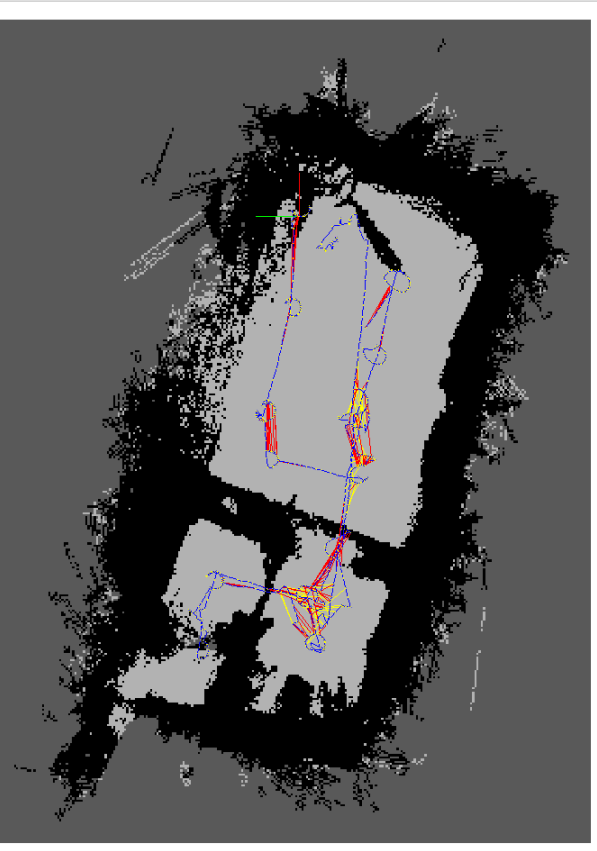
\includegraphics[height=6cm]{Images/mapping graph.png}
    \caption{Mapping Graph}
    \label{fig:mapping_graph}
\end{figure}

\subsubsection{SLAM Limitations and Hybrid Approach Development}

Initial testing of pure RTABMap implementation revealed critical limitations that motivated the development of a hybrid sensor fusion approach. Extended operation testing documented position drift accumulation reaching up to 1.2 meters during 30-minute sessions, with gradual error accumulation particularly pronounced in feature-poor environments or areas with repetitive visual patterns.

Error analysis identified visual odometry drift as the primary contributor, exacerbated by lighting changes, motion blur during movement, and insufficient visual features near walls. Statistical analysis revealed systematic bias in specific movement directions with standard deviations exceeding 40cm for identical positioning commands. Relocalization failures occurred frequently in environments with insufficient distinctive features, requiring manual intervention through robot rotation and often complete database reconstruction when loop closure detection failed catastrophically.

These limitations proved particularly problematic for VR applications requiring precise robot positioning, necessitating the integration of Ultra-Wideband positioning for absolute position reference.

\subsubsection{UWB Positioning System Integration}

The Ultra-Wideband positioning system addresses SLAM drift limitations by providing absolute position reference with centimeter-level accuracy. The UWB integration utilizes the \texttt{uwb\_positioning} package configured through \texttt{uwb.launch.py} with serial communication parameters \texttt{serial\_port\_name: /dev/ttyACM0} and \texttt{serial\_baud\_rate: 115200} for DecaWave hardware interface.

Strategic anchor placement ensures optimal coverage while minimizing Non-Line-of-Sight conditions. The system implements multilateration techniques calculating 3D position from time-of-flight measurements to multiple anchor points.

Position data publishes on \texttt{/UWB/Pos} using \texttt{geometry\_msgs/Pose} format, providing absolute 3D coordinates that serve as the reference for sensor fusion algorithms.

\subsubsection{Hybrid Sensor Fusion Architecture}

The hybrid localization system combines the complementary strengths of visual SLAM and UWB positioning through sophisticated sensor fusion that separates position and orientation estimation. This approach utilizes UWB for absolute position reference while maintaining RTABMap for orientation data, addressing the limitations of each individual system.

\paragraph{Fusion Algorithm Implementation}

The \texttt{\_create\_fused\_pose} method implements core fusion logic prioritizing UWB position data when available, with automatic fallback to RTABMap position estimates during UWB communication failures. Position data undergoes coordinate frame transformation using a configurable 11.5-degree rotation correction through the \texttt{\_apply\_rotation\_to\_pose} method, aligning UWB coordinates with the RTABMap reference frame.

Orientation estimation maintains RTABMap quaternion data as the primary source with validation to detect loss conditions. The system monitors for invalid quaternion values (x=1.0, y=0.0, z=0.0, w=0.0) indicating RTABMap odometry failure and automatically triggers the \texttt{/reset\_odom} service while maintaining position tracking through UWB data.

\paragraph{Orientation Recovery and Fallback Mechanisms}

During RTABMap orientation loss, the \texttt{\_estimate\_orientation\_from\_movement} method calculates orientation from position history, storing the last 5 position measurements with minimum 5cm movement thresholds. Recovery validation continuously monitors RTABMap orientation data, automatically transitioning back upon detection of valid orientation values while maintaining UWB position data.

Performance monitoring tracks sensor health, fusion quality, and system reliability through comprehensive statistics on UWB availability, RTABMap orientation validity, and fusion algorithm performance.

The resulting hybrid system provides robust localization that maintains the accuracy advantages of UWB positioning while preserving the orientation capabilities of visual SLAM, establishing the foundation for precise human detection and interaction positioning described in the following subsection.



\subsection{Human Pose Detection with YOLOv11 and TensorRT Optimization}

Effective human-robot interaction requires real-time human pose detection that can identify body positions, gestures, and spatial relationships in dynamic social environments. The computational demands of deep learning-based pose detection on embedded hardware necessitate careful optimization strategies to achieve real-time performance while maintaining detection accuracy for social robotics applications.

\subsubsection{YOLOv11n-Pose Model Selection and TensorRT Optimization}

The YOLOv11n-pose model provides optimal balance between detection accuracy and computational efficiency for the NVIDIA Orin Nano platform. The nano variant utilizes a streamlined architecture with reduced parameter count, enabling real-time inference while maintaining adequate accuracy for social robot interaction requirements and multi-person detection capabilities within the camera's field of view.

Pre-trained model weights eliminate extensive training requirements by leveraging established pose estimation datasets, providing immediate deployment capability with robust performance across diverse human poses and environmental conditions typical of social robot applications.

\paragraph{Model Format Conversion and Engine Optimization}

The optimization pipeline transforms the original \texttt{yolo11n-pose.pt} PyTorch format through sequential conversions: ONNX intermediate format (\texttt{.onnx}) for cross-platform compatibility, followed by TensorRT engine generation (\texttt{.engine}) for hardware-specific optimization. TensorRT optimization analyzes the YOLOv11n-pose network structure and generates optimized CUDA kernels that maximize GPU utilization through layer fusion, precision calibration, and memory access optimization.

Engine generation includes precision optimization techniques evaluating network sensitivity to reduced precision arithmetic, potentially utilizing INT8 quantization while maintaining FP16 or FP32 precision for critical layers requiring higher numerical accuracy. Memory allocation strategies optimize GPU memory usage patterns to prevent fragmentation and minimize allocation overhead during inference operations.

Performance benchmarks on NVIDIA Jetson Orin Nano demonstrate significant optimization gains: TensorRT FP16 achieves 4.53ms inference time compared to 13.70ms for PyTorch format, representing a 3x performance improvement while maintaining mAP50--95 accuracy of 0.5061 versus 0.5101 for the original model. TensorRT INT8 optimization further reduces inference time to 3.70ms with mAP50--95 of 0.4825, providing optimal performance for real-time applications where slight accuracy reduction is acceptable for substantial speed gains.

\subsubsection{ROS2 Pose Detection Node Architecture}

The \texttt{pose\_detection\_node.py} integrates seamlessly with Tino's ROS2 architecture, managing camera input, TensorRT inference execution, and structured result publication for downstream processing systems.

\paragraph{Camera Integration and Preprocessing}

The node subscribes to Oak-D Pro topics \texttt{/right/image\_rect} for monocular RGB input and \texttt{/stereo/depth} for corresponding depth information required for 3D coordinate calculation. Image preprocessing includes monocular to BGR conversion for YOLO compatibility using CPU-based OpenCV operations while maintaining real-time performance through efficient memory management.

Synchronization mechanisms maintain temporal alignment between RGB and depth streams through callback-based processing with \texttt{latest\_image} and \texttt{latest\_depth\_image} synchronization, ensuring corresponding depth information availability for each processed RGB frame.

\paragraph{TensorRT Inference and Result Processing}

TensorRT inference utilizes the pre-converted \texttt{yolo11n-pose.engine} model loaded through \texttt{YOLO(model\_path)} initialization with configurable confidence thresholding (default 0.5) and \texttt{verbose=False} parameter. Post-processing extracts pose keypoints, confidence scores, and bounding box information from \texttt{results[0]} objects, implementing confidence-based filtering and closest person selection based on depth measurements.

Error handling provides comprehensive exception management with detailed logging at configurable levels and graceful degradation during model loading failures or inference errors, maintaining operational continuity through robust try-catch blocks around critical processing sections.

The pose detection results feed directly into the 3D positioning system described in the following subsection, enabling spatial localization of detected human poses.

\subsection{Stereo Depth Integration for 3D Human Positioning}

Accurate spatial awareness requires combining 2D pose detection results with precise depth information to enable 3D human positioning capabilities essential for spatial interaction planning and safety monitoring in social robotics applications.

\subsubsection{Oak-D Pro Depth Processing and Validation}

The Oak-D Pro stereo system generates depth maps through stereo vision algorithms, with depth accuracy depending on stereo baseline, camera calibration quality, and environmental factors including lighting conditions and surface textures.

\paragraph{Robust Depth Extraction}

Depth value extraction implements a median-based approach with a 9x9 pixel window around keypoint locations to obtain robust measurements. The \texttt{get\_depth\_at\_point} function performs outlier filtering by calculating median and standard deviation, filtering values more than 2 standard deviations from the median to ensure reliable depth extraction.

For person detection, the \texttt{get\_median\_depth} function extracts depth from a central bounding box region with configurable padding (25\% by default), providing more stable measurements than single-pixel sampling while avoiding background contamination. Depth validation implements comprehensive quality filtering including zero-value rejection, outlier detection based on statistical analysis, and temporal smoothing over a configurable window size (default 3 frames).

\paragraph{3D Coordinate Transformation}

The \texttt{calculate\_3d\_position} function converts camera-frame coordinates using intrinsic parameters from the \texttt{camera\_info.k} array, extracting focal lengths \texttt{fx}, \texttt{fy} and principal point coordinates \texttt{cx}, \texttt{cy} from the calibration matrix. Automatic unit conversion detects depth values greater than 100 for millimeter to meter conversion, followed by depth calibration correction using configurable \texttt{depth\_scale\_factor} (default 0.575) and \texttt{depth\_offset} parameters derived from empirical calibration.

3D coordinate calculation applies the standard pinhole camera model: \texttt{x\_3d = (x - cx) * z / fx} and \texttt{y\_3d = (y - cy) * z / fy}, where corrected depth \texttt{z = z * depth\_scale\_factor + depth\_offset} accounts for systematic depth measurement biases in the Oak-D Pro stereo system.

\subsubsection{3D Skeleton Generation with Temporal Consistency}

The 3D skeleton generation process combines 2D keypoint detections with corresponding depth values to create complete spatial human pose representations with temporal stability for real-time applications.

\paragraph{Keypoint Depth Association and Validation}

Depth value assignment utilizes 2D keypoint pixel coordinates to extract corresponding depth measurements from the stereo depth map with validation ensuring measurements correspond to human body parts rather than background objects. The \texttt{process\_skeleton} function implements sophisticated temporal smoothing where individual keypoint depths are validated against a reference depth calculated as the median of all valid keypoint depths.

Outlier rejection filters keypoint depths deviating more than the configurable \texttt{depth\_outlier\_threshold} (default 30\%) from the reference, replacing them with temporal median depth from a smoothing window. Missing depth handling addresses invalid keypoint scenarios through reference depth fallback when coordinates are invalid ($x \leq 0$ or $y \leq 0$) or depth extraction fails.

Temporal smoothing maintains a \texttt{skeleton\_depth\_history} list with configurable window size (default 3 frames) storing reference depths for median filtering over time, providing stable depth values that reduce measurement jitter while maintaining responsiveness to actual depth changes.

The resulting 3D skeleton data enables comprehensive real-time tracking capabilities, as detailed in the following subsection describing the complete skeleton tracking implementation.



\subsection{Real-time Skeleton Tracking with COCO Keypoint Framework}

Complete human understanding in social robotics requires comprehensive skeleton tracking that captures body posture, gesture recognition, and movement patterns. The standardized COCO keypoint framework provides a robust foundation for consistent pose representation, enabling reliable gesture analysis and human behavior understanding essential for natural human-robot interaction.

\subsubsection{17-Keypoint COCO Detection Schema}

The implementation utilizes the established COCO pose estimation standard identifying 17 key body joints: nose (0), left eye (1), right eye (2), left ear (3), right ear (4), left shoulder (5), right shoulder (6), left elbow (7), right elbow (8), left wrist (9), right wrist (10), left hip (11), right hip (12), left knee (13), right knee (14), left ankle (15), and right ankle (16).

Joint indexing follows established COCO conventions ensuring compatibility with existing pose analysis tools and datasets, enabling straightforward integration with pose analysis algorithms and facilitating comparison with other human pose detection systems. Keypoint connectivity defines skeletal structure through predefined joint relationships representing human anatomical connections including head structure (nose-eyes-ears), torso connections (shoulders-hips), and limb chains (shoulder-elbow-wrist, hip-knee-ankle) that enable skeletal validation and pose completeness assessment.

\paragraph{Confidence Scoring and Quality Assessment}

Confidence score extraction provides reliability metrics for each detected keypoint, with values ranging from 0.0 (undetected) to 1.0 (high confidence) indicating detection algorithm certainty in keypoint localization accuracy. Quality thresholding implements confidence-based filtering excluding low-confidence detections from downstream processing, with threshold values balancing detection completeness against accuracy requirements typically ranging from 0.3 to 0.7 depending on application requirements and environmental conditions.

Multi-person confidence handling manages confidence scores when multiple humans are detected simultaneously, maintaining separate confidence profiles for each detected person while implementing consistency checks ensuring skeletal coherence within individual pose detections.

\subsubsection{Data Processing Pipeline and Skeleton Organization}

The data processing pipeline transforms raw YOLOv11 output into structured skeleton representations suitable for real-time robot applications through coordinate extraction, normalization, and validation procedures.

\paragraph{Coordinate Processing and Validation}

Raw network output processing extracts keypoint coordinates and confidence scores from YOLOv11 inference results, handling variable-length outputs accommodating different numbers of detected humans while maintaining consistent data structures. Coordinate normalization converts pixel coordinates to standardized coordinate systems enabling consistent processing regardless of camera resolution or field of view variations.

Geometric consistency validation implements anatomical constraints verifying reasonable joint relationships within detected skeletons, including bone length checks, joint angle limitations, and bilateral symmetry assessments that identify and filter implausible pose detections. Temporal consistency analysis compares consecutive pose detections to identify and smooth measurement noise while detecting rapid pose changes indicating genuine human motion.

Completeness assessment evaluates skeleton quality based on the number and distribution of successfully detected keypoints, with assessment criteria including minimum keypoint requirements, critical joint detection (head, torso, limbs), and pose coverage metrics indicating skeleton suitability for specific applications.

\subsubsection{ROS2 Integration and Multi-Modal Data Publishing}

The skeleton tracking system publishes comprehensive pose data through multiple ROS2 topics enabling integration with various robot systems and applications, providing different data formats optimized for specific use cases.

\paragraph{Multi-Topic Publishing Architecture}

The system implements specialized publishers for different data requirements: \texttt{/pose\_detection/image\_raw} for annotated detection images enabling visual debugging, \texttt{/human\_position} for smoothed human position using \texttt{PoseStamped} messages optimized for robot controller integration, \texttt{/human\_skeleton} for 3D skeleton visualization using \texttt{MarkerArray} messages suitable for RViz display, and \texttt{/human\_skeleton\_poses} for programmatic access to joint coordinates using \texttt{PoseArray} messages.

Multi-person handling focuses on closest person selection based on depth measurements, identifying the person with minimum depth value and processing only that individual's skeleton data. This approach reduces computational overhead while ensuring consistent tracking of the most relevant human for interaction applications, with automatic selection providing safety prioritization.

Timestamp synchronization utilizes \texttt{self.get\_clock().now().to\_msg()} for all published messages with consistent \texttt{header.frame\_id} set to the configurable camera frame (default: \texttt{oak\_right\_camera\_optical\_frame}), ensuring temporal alignment across all pose-related data streams.

\paragraph{Robot Controller and VR System Integration}

Robot controller integration subscribes to \texttt{/human\_position} topic for spatial awareness applications where human position data undergoes temporal smoothing through the \texttt{publish\_human\_position} function maintaining a configurable history buffer (default 5 positions) and publishing averaged coordinates to reduce measurement jitter while maintaining responsiveness to human movement.

Pose-based behavior triggers utilize multiple data streams including raw skeleton data from \texttt{/human\_skeleton\_poses} for detailed joint analysis, smoothed position data from \texttt{/human\_position} for proximity detection, and visual markers from \texttt{/human\_skeleton} for debugging and visualization purposes. Safety monitoring implementation prioritizes closest person detection ensuring safety systems focus on the most immediate interaction partner.

VR system integration transmits skeleton data through the dedicated \texttt{vr\_interface\_node.py} described in the software architecture, utilizing the three-port UDP protocol (port 5007 for 208-byte skeleton data at 10Hz) for immersive visualization and interaction analysis. The VR interface node formats skeleton data for Unity applications using the established COCO-format structure with exactly 17 joints, applying default (0,0,0) coordinates for missing joints to maintain data consistency. Data recording capabilities capture complete skeleton tracking sessions for offline analysis through synchronized pose data, camera images, and robot state information published across the multi-topic ROS2 architecture.

The comprehensive skeleton tracking system provides the spatial and temporal human understanding necessary for sophisticated social robot behaviors, with the multi-modal data publishing architecture supporting both real-time robot control and offline analysis requirements for continued system improvement.




\section{Control Architecture: From Perception to Physical Response}
\label{sec:control_implementation}
Real-time VR teleoperation demands precise translation of user intentions into robot movements while maintaining spatial awareness and natural social behaviors. The challenge extends beyond simple command forwarding: the system must coordinate multiple actuators, ensure movement completion, handle network uncertainties, and maintain synchronization between leg expressions and base locomotion. This section details the control implementation that transforms perception inputs (from Section~\ref{sec:perception_sensing}) into coordinated physical responses through the hardware interfaces described in Section~\ref{sec:hardware_impl}.

The control system addresses three fundamental requirements: (1) guaranteed movement completion to prevent incomplete gestures that compromise social interaction, (2) temporal coordination between multiple actuators to create coherent robot behaviors, and (3) robust VR communication that handles network latency and packet loss without degrading user experience.

\subsection{Atomic Movement Framework: Ensuring Predictable Robot Behavior}

Traditional continuous control architectures suffer from unpredictable interruptions that can leave robots in intermediate states, particularly problematic for social robots where incomplete gestures appear unnatural or confusing to human observers. The atomic movement system addresses this by implementing discrete, completion-guaranteed movements that provide deterministic correspondence between VR user intentions and physical robot actions.

The unified 4-state framework standardizes behavior across both leg and base controllers, enabling sophisticated coordination while maintaining implementation simplicity. The design builds upon the legacy Tino system's proven movement patterns, adapting continuous expressive movements into discrete, completion-guaranteed states that provide deterministic correspondence between VR user intentions and physical robot actions.

\subsubsection{Design Rationale Based on Legacy System Experience}

The 4-state architecture emerged from practical experience with the original Tino robot's social interaction capabilities demonstrated by Cardillo~\cite{cardillo2024thesis}. The legacy system demonstrated that specific movement characteristics successfully conveyed intentionality and lifelike behavior during human-robot interaction experiments, particularly the coordinated synchronization between base movement, leg extension patterns, and upper-body tilting that created a unified sense of effort and purposeful motion. The timing parameters and movement patterns implemented in Tino V2 preserve these successful interaction dynamics while restructuring them into atomic operations suitable for VR teleoperation.

The discrete state approach addresses three critical requirements identified from the legacy system's operation: \textbf{predictable movement completion} to prevent the incomplete gestures that compromised social presence in continuous control scenarios, \textbf{coordinated multi-actuator behavior} that creates coherent robot expressions rather than separate mechanical operations, and \textbf{reliable VR command processing} that maintains responsiveness without command accumulation or timing conflicts.

\subsubsection{State 0: Neutral Positioning and System Ready}
The idle state maintains system readiness while implementing intelligent auto-positioning for the leg controller. The differentiated RPM values (110 forward, 70 backward, 90 neutral) are derived from empirical testing of the Tino V2 system to optimize the motor characteristics for social interaction, where forward extensions appear more deliberate while return movements exhibit gentler characteristics, building upon the movement principles established in the original Tino's expressive capabilities. The 50-tick tolerance zone accommodates normal system vibration while preventing micro-adjustments that would appear nervous or uncertain. The base controller implements complete motion cessation with comprehensive flag reset, ensuring clean state transitions that provide clear visual cues for state changes.

\subsubsection{State 1: Expressive Attention Behaviors}
Attention-getting movements provide non-verbal communication capabilities essential for social interaction. The 3-phase timing (50\%--5\%--45\% over 1.2 seconds) implements a new ``little push'' movement developed for Tino V2 that incorporates the attention-capture principles demonstrated in the original Tino's social interaction experiments. The brief 5\% pause creates anticipation and draws human attention more effectively than continuous motion, following the expressive movement patterns that proved successful in the legacy system's collaborative tasks. The base controller's ``nudging'' behavior (600ms preparation, 200ms forward, 200ms return) creates a subtle forward lean that maintains spatial positioning while conveying directional intent, preserving the deliberate movement characteristics that facilitated successful human-robot communication in the original experiments.

\subsubsection{State 2: Coordination Preparation}
Multi-component movement coordination requires temporal synchronization to create coherent robot behaviors that appear as unified intentions rather than separate mechanical operations. The leg controller's maximum extension followed by PID hold (Kp=2.0, Ki=0.1, Kd=0.5) creates visual preparation that signals impending coordinated movement, building upon the synchronized base-leg movements that successfully conveyed effort and intentionality in the original Tino system~\cite{cardillo2024thesis}. The base controller's 1.5-second timing cycle provides sufficient coordination time while maintaining the perception of responsive control, optimized for the discrete state system while preserving the coordinated movement principles established in the legacy experiments.

\subsubsection{State 3: Coordinated Movement Execution}
The final phase executes completion-guaranteed operations with movement parameters that preserve the social interaction effectiveness demonstrated in the original Tino experiments~\cite{cardillo2024thesis}. The leg controller's return to neutral using tactile feedback (home button detection) provides the precise positioning essential for movement completion while maintaining the controlled motion characteristics that created successful human-robot interaction in collaborative scenarios. The 1.7-second base movement duration preserves the deliberate, effortful movement quality that proved effective for conveying intentionality in social scenarios, as demonstrated in the legacy system's experimental validation. The three angular movement options (forward=0, right=1, left=-1) provide sufficient directional capability while maintaining simple cognitive mapping for VR operators, based on the movement vocabulary that successfully supported collaborative tasks in the original experiments.

\subsubsection{Legacy-to-VR Adaptation Rationale}

The transition from the legacy system's continuous, manually-controlled movements to Tino V2's discrete atomic states preserves the essential movement characteristics that proved successful for social interaction while adapting them for VR teleoperation requirements. The original system's effective movement patterns---including the ``dragging'' leg motion, coordinated upper-body tilting, and deliberate timing that fostered empathy and trust in human-robot interaction scenarios~\cite{cardillo2024thesis}---are encapsulated within the 4-state framework to maintain the social presence and expressive capabilities that made the original Tino successful in collaborative tasks.

This adaptation approach ensures that the proven social robotics capabilities are preserved while gaining the benefits of atomic movement completion, VR responsiveness, and systematic coordination that enable advanced teleoperation scenarios. The framework successfully bridges legacy interaction effectiveness with modern control requirements, providing the foundation for natural human-robot interaction through advanced VR integration.

\subsubsection{Technical Implementation Details}

The control system employs two key mechanisms to ensure precise and reliable robot movement. First, the positioning system uses absolute encoders that track exact component positions, similar to how a GPS provides precise location data. However, the robot's mechanical components do not behave identically in all directions due to factors such as friction, weight distribution, and gear backlash. To address this asymmetry, the system applies calibrated scaling factors: forward movements use a multiplier of 1.15 while backward movements use 0.85, effectively compensating for the mechanical differences and ensuring consistent movement distances regardless of direction.

Second, the movement coordination system prevents conflicts between simultaneous operations through a timing-based approach. The base controller's \texttt{updateBaseMovement}\linebreak\texttt{ByTime()} function operates with millisecond precision, using a locking mechanism (\texttt{isCase}\linebreak\texttt{2Locked}) that functions like a traffic light system. When one movement sequence begins, the lock prevents new commands from interrupting until the current operation completes entirely. This ensures that each movement executes fully and predictably, which is essential for maintaining the robot's social interaction capabilities and preventing the jerky or incomplete movements that would appear unnatural to human observers.

\subsection{Signal Processing: From VR Intent to Robot Command}

VR teleoperation requires robust signal processing to handle the inherent challenges of wireless communication, user input variability, and real-time processing constraints. The system transforms continuous VR inputs into discrete robot commands while maintaining responsiveness and preventing command accumulation that could lead to unpredictable robot behavior.

\subsubsection{Pulse-Based Command Architecture}

The communication between VR systems and the robot employs a pulse-based architecture that solves critical problems inherent in continuous control systems. Instead of transmitting signals continuously while buttons are pressed (which could accumulate in network buffers or create timing dependencies), the system implements discrete command pulses that provide guaranteed one-to-one correspondence between user actions and robot movements.

\textbf{The Core Problem}: Traditional continuous control systems suffer from command accumulation when network latency varies or when users hold buttons for extended periods. For example, if a user presses a movement button and network delays cause commands to queue up, the robot might continue executing movements long after the user releases the button, creating unpredictable and potentially dangerous behavior.

\textbf{The Pulse Solution}: Each VR interaction triggers exactly three identical command cycles transmitted automatically, regardless of how long the user holds the input. This approach guarantees that one button press equals one complete robot movement sequence, with automatic return to idle state preventing command accumulation.

\subsubsection{Implementation Details with Concrete Examples}

The pulse architecture operates through a systematic three-phase transmission cycle that can be observed in both the gamepad controller (used for development testing) and the VR interface node. 

\textbf{Gamepad Implementation Example}: When a user presses the X button (corresponding to State 1 - ``little push'' movement), the \texttt{gamepad\_node.py} executes the following sequence:

\begin{verbatim}
# Button press triggers pulse initiation
def trigger_leg_command_pulse(self, command):
    self.leg_command_pulse_target = command  # Set target to 1
    self.leg_command_pulse_count = 0         # Reset counter
    self.leg_command = command               # Immediate activation

# Timer callback executes at 25Hz (every 40ms)
def publish_commands(self):
    if self.leg_command_pulse_count < 3:     # Send 3 cycles
        self.leg_command = self.leg_command_pulse_target
        self.leg_command_pulse_count += 1
        
        if self.leg_command_pulse_count >= 3:
            self.leg_command = 0             # Auto-return to idle
            self.leg_command_pulse_target = -1
\end{verbatim}

This produces exactly three ROS2 messages at 40ms intervals (120ms total duration), each containing \texttt{base\_cmd.linear.x = 1.0}, followed by automatic return to \texttt{base\_cmd}\linebreak\texttt{.linear.x = 0.0} (idle state).

\textbf{VR Interface Implementation}: The VR system uses identical timing through UDP packet processing. When Unity sends a VR command packet, the \texttt{vr\_interface\_node.py} receives a 32-byte binary structure:

\begin{verbatim}
# Incoming UDP packet format (32 bytes total)
data = struct.unpack('fffiiffi', received_data)
# [head_pitch, head_pan, head_tilt, base_state, base_angular, 
#  audio_volume, audio_orientation, message_order]

# Example: State 2 command with right rotation
# [0.0, 0.0, 0.0, 2, 1, 75, 0.0, 12345]
\end{verbatim}

The VR interface processes these commands identically to gamepad pulses, ensuring that VR development accurately represents final system behavior. Unity applications send single command packets when users perform actions, and the ROS2 system automatically generates the three-cycle pulse sequence with guaranteed completion.

\textbf{Timing Coordination with Robot States}: The 120ms pulse duration is specifically designed to coordinate with the robot's atomic movement states. State 2 (coordination preparation) has a 1.5-second duration, during which the pulse system can process multiple incoming commands without conflicts. Commands received during active movements are queued and automatically executed upon completion, maintaining the atomic guarantee while providing responsive user feedback.

\subsubsection{Network Reliability and Message Validation}

The pulse system incorporates sophisticated reliability mechanisms to handle real-world network conditions. Each UDP packet includes a 32-bit message order counter that enables duplicate detection and lost packet monitoring:

\begin{verbatim}
# Message ordering validation in vr_interface_node.py
expected_order = (self.last_message_order + 1) % (2**31)
if message_order != expected_order:
    if message_order == self.last_message_order:
        return  # Skip duplicate messages
    else:
        self.get_logger().warn(f'Order gap: Expected {expected_order}, 
                               Received {message_order}')
\end{verbatim}

The three-cycle repetition provides redundancy against packet loss: if one of the three 40ms transmissions fails due to network interruption, the remaining cycles ensure command delivery. Parameter consistency checking across all three pulses validates command integrity, rejecting corrupted or incomplete transmissions.

This architecture maintains communication reliability while avoiding the overhead of TCP acknowledgments that would introduce unacceptable latency for real-time VR control. The 120ms total duration exceeds typical network latency variations (usually <50ms on local networks) while preventing command accumulation that could compromise movement predictability.

\subsubsection{Input Signal Conditioning}
VR input processing transforms continuous controller actions into discrete events through rising-edge triggering on button activation, preventing continuous command generation during extended button holds that could overwhelm the robot's movement capabilities. Input debouncing requires 200ms minimum intervals between commands, while the system captures and encodes current VR state (head orientation) at command initiation time, ensuring movement commands reflect the user's spatial context when the action was initiated.

The identical pulse generation system enables development testing through gamepad control that accurately represents VR operational behavior. Gamepad button mapping follows VR command structure: face buttons control leg states (X→state 1, Y→state 2, B→state 3, A→idle), while shoulder buttons enable combined movement testing with simultaneous angular direction commands.

\subsection{Unity-ROS2 Communication Protocol}

The VR integration relies on optimized UDP communication between Unity VR applications and the ROS2 control system, designed to minimize latency while maintaining data integrity and providing robust error handling for production use.

\subsubsection{Message Structure and Processing}
UDP packet processing extracts commands from compact 32-byte binary structures using \texttt{struct.unpack('fffiiffi', data)} format, optimized for minimal bandwidth usage while providing comprehensive control data. The packet format consists of three consecutive 32-bit floats for head control (pitch, pan, tilt), two 32-bit integers for base commands (state 0-3, angular direction -1/0/1), two additional fields for audio control (volume as integer, orientation as float), and a final 32-bit integer for message ordering. This structure enables atomic unpacking with deterministic field extraction while maintaining fixed-size packets that simplify buffer management and reduce parsing overhead.

Head commands (pitch, pan, tilt) forward directly to robot controllers for immediate response, while base commands (state 0-3, angular -1/0/1) trigger atomic movement execution through the unified 4-state framework detailed in Section~\ref{sec:control_implementation}. The system implements comprehensive packet validation including exact size verification (32 bytes), structural integrity checking through Python's \texttt{struct.unpack()} exception handling, and range validation for critical parameters such as base state bounds (0-3) and angular direction constraints (-1,0,1).

\subsubsection{Advanced Message Ordering and Validation}

Message ordering employs sophisticated 32-bit sequence numbers that provide comprehensive duplicate detection and lost packet monitoring capabilities essential for reliable VR teleoperation. The system implements a three-tier validation architecture that addresses the unique challenges of UDP communication in real-time robotics applications.

\textbf{Sequence Number Management}: Each incoming UDP packet contains a monotonically increasing 32-bit message order counter that enables precise tracking of communication patterns. The system maintains \texttt{last\_message\_order} state with automatic wraparound handling using modulo arithmetic \texttt{(last\_order + 1) \% (2**31)} to prevent integer overflow while preserving ordering semantics. This approach provides over 2 billion unique sequence numbers before wraparound, sufficient for continuous operation exceeding 24 hours at 25Hz transmission rates.

\textbf{Duplicate Detection Algorithm}: The validation system implements intelligent duplicate filtering by comparing incoming sequence numbers against expected values. When \texttt{message\_order <= last\_message\_order} and the value is positive, the system identifies potential duplicates or out-of-order packets and logs warnings while skipping packet processing to prevent command repetition. This mechanism prevents movement accumulation caused by network-level packet duplication or VR system retransmission attempts.

\textbf{Gap Detection and Loss Monitoring}: Lost packet detection operates through gap analysis where \texttt{message\_order != expected\_order} triggers warning logs that include both expected and received values for diagnostic purposes. The system distinguishes between minor gaps (1-3 missing packets, typically acceptable for real-time control) and major gaps (>10 missing packets, indicating significant network issues) through configurable thresholds. Gap information enables network quality assessment and adaptive control strategies that can adjust transmission rates or implement backup communication protocols during degraded network conditions.

\subsubsection{Comprehensive Communication Health Monitoring}

The system implements multi-layered communication health monitoring that provides continuous assessment of VR-robot communication quality through statistical analysis, rate validation, and connection status tracking. This monitoring architecture enables proactive detection of communication degradation before it impacts robot operation.

\textbf{Rate-Based Health Assessment}: The monitoring system tracks actual versus expected communication rates through configurable parameters including \texttt{expected\_receiv}\linebreak\texttt{e\_rate\_hz} (default 25Hz for VR commands), \texttt{pose\_send\_rate\_hz} (default 10Hz for robot pose data), and \texttt{skeleton\_send\_rate\_hz} (default 10Hz for human tracking). The system maintains sliding-window statistics over configurable intervals (default 10 seconds) that calculate actual transmission rates using \texttt{packet\_count / time\_period} calculations. Rate deviations exceeding configurable thresholds (typically 20\% for incoming data, 10\% for outgoing data) trigger graduated warning levels that help distinguish between temporary network fluctuations and systematic communication failures.

\textbf{Connection Status and Timeout Management}: Advanced connection tracking implements sophisticated timeout mechanisms with configurable disconnection thresholds (default 3 seconds) that account for typical network latency variations. The system maintains \texttt{is\_vr\_connected} state through timestamp comparison using \texttt{current\_time - last\_received\_time > disconnection\_timeout} logic. Connection state transitions trigger automatic recovery procedures including message order counter reset (\texttt{last\_messa}\linebreak\texttt{ge\_order =-1}) for graceful reconnection handling.

\textbf{Adaptive Monitoring and Recovery}: The health monitoring system implements adaptive behavior based on connection history and communication patterns. During stable operation, monitoring logs are generated at configurable intervals (default 10 seconds) with information-level messages confirming normal operation. When communication issues are detected, the system increases logging frequency and detail level while implementing automatic recovery procedures. Upon VR reconnection, the system logs reconnection events, resets sequence counters to handle Unity application restarts gracefully, and provides startup confirmation that enables operators to verify communication restoration.

\textbf{Statistical Analysis and Trend Detection}: The monitoring system maintains comprehensive statistics including total packet counts, rate calculations over multiple time windows, and trend analysis for early detection of degrading communication quality. Metrics include successful packet reception rates, sequence gap frequency, and timing consistency measurements that enable predictive maintenance and network optimization. This statistical foundation supports both real-time operation decisions and long-term system optimization through data-driven communication tuning.

\subsubsection{Performance and Reliability Characteristics}
The communication system is designed to maintain low latency for real-time VR teleoperation while ensuring atomic movement commands complete reliably even under network stress conditions. The system prioritizes head movement responsiveness to provide immediate visual feedback, while atomic movement commands are optimized for reliable initiation and completion according to their predefined state timings. 

Error recovery mechanisms automatically detect VR disconnection and implement safe robot shutdown procedures, preventing autonomous operation that could pose safety risks. The comprehensive monitoring and validation framework provides operators with detailed insight into communication health while maintaining the sub-50ms latency requirements essential for natural VR interaction.

The control architecture successfully bridges the gap between VR user intentions and coordinated robot responses, providing the foundation for natural human-robot interaction through the advanced perception capabilities detailed in Section~\ref{sec:perception_sensing}. The atomic movement system ensures predictable robot behavior essential for social interaction, while the pulse-based communication protocol maintains real-time responsiveness required for effective VR teleoperation.


\section{System Integration}
\label{sec:integration_implementation}

Complex robotics systems achieve their full potential only through seamless integration of their constituent subsystems. While individual components may function correctly in isolation, the coordination between hardware controllers, software nodes, perception algorithms, and external interfaces determines whether the system operates as a unified platform or remains a collection of disconnected modules. This chapter presents the integration methodology that transforms the Tino V2's diverse components into a cohesive VR-embodied robotic system capable of real-time social interaction.

The integration challenges extend beyond simple component interconnection. The system must coordinate multiple Arduino controllers operating at different speeds, synchronize perception data from various sensors, maintain real-time communication with VR systems, and ensure that atomic movement commands execute reliably despite network latencies and computational loads. Additionally, the integration must support both development workflows—where individual subsystems require isolated testing—and production deployment where all components operate simultaneously.

\subsection{System Architecture Integration}

The integration methodology addresses the fundamental challenge of coordinating diverse subsystems that operate across different computational platforms, communication protocols, and timing requirements. The solution employs a layered architecture where ROS2 serves as the central coordination layer, managing communication between hardware interfaces, perception modules, and external systems while maintaining modularity for development and debugging.

\subsubsection{ROS2 Node Orchestration}

The distributed ROS2 architecture enables sophisticated parallel processing while maintaining reliable inter-node communication through the Data Distribution Service middleware. The six primary nodes—gamepad control, hardware interface, robot controller, pose detection, VR interface, and UWB positioning—operate as independent processes that communicate through standardized message interfaces, enabling optimal utilization of the Orin Nano's multi-core architecture.

Node interdependencies follow a carefully designed communication graph that prevents circular dependencies while enabling rich data sharing. The robot controller node serves as the central coordination hub, receiving localization data from RTABMap, absolute positioning from UWB, and movement commands from either gamepad or VR interface nodes. This centralized approach enables sophisticated sensor fusion and behavior coordination while maintaining loose coupling between subsystems.

Launch file orchestration manages the complex startup sequence required for reliable system initialization. The \texttt{start\_tino\_with\_rtab.launch.py} configuration implements staged initialization where camera and IMU systems initialize first, followed by SLAM nodes, then hardware interfaces, and finally VR communication nodes. This sequencing prevents initialization race conditions while ensuring that critical dependencies like camera calibration and IMU orientation are established before dependent systems come online.

Quality of Service (QoS) policies optimize communication reliability for different data types: sensor data utilizes ``best effort'' delivery for maximum throughput, control commands employ ``reliable'' delivery to ensure execution, and system health monitoring uses ``transient local'' durability to maintain state information across node restarts. These differentiated QoS policies enable optimal performance while maintaining system reliability.

\subsubsection{Hardware-Software Interface Coordination}

The integration between software control systems and physical hardware requires sophisticated coordination to handle the disparate timing characteristics of Arduino controllers, ROS2 nodes, and VR systems. The hardware interface node implements thread-based communication management that maintains independent serial connections to three Arduino controllers while coordinating their combined operation through centralized command generation.

\begin{figure}[H]
    \centering
    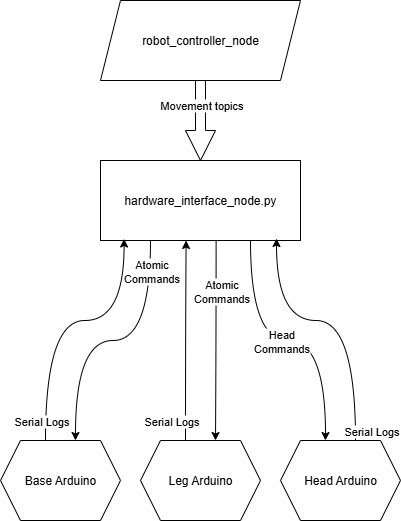
\includegraphics[height=6cm]{Images/HardwareNodeInteraction.png}
    \caption{Hardware Interface Node Communication Architecture}
    \label{fig:hardware_node_interaction}
\end{figure}

Serial communication reliability employs several integration strategies to ensure robust operation. Persistent device naming through udev rules (\texttt{/dev/ttyBASE}, \texttt{/dev/ttyLEG}, \texttt{/dev/ttyHEAD}) eliminates device enumeration variability that could disrupt system startup. Triple-redundant command transmission at the protocol level ensures message delivery across communication disruptions, while thread-based connection monitoring enables automatic reconnection without affecting other subsystem operations.

The atomic movement coordination system demonstrates sophisticated integration between software control logic and hardware execution timing. State transitions must coordinate between leg extensions (requiring encoder feedback) and base movements (using timer-based control) while handling the different response characteristics of each subsystem. The integration ensures that compound movements like ``extend leg, move base, retract leg'' execute as atomic operations despite involving multiple physical controllers with independent timing requirements.

Command format standardization through the key-value protocol (\texttt{BF=value,BB=value,}\linebreak\texttt{HP=value,HX=value,HY=value}) enables unified control message generation while accommodating the different parameter requirements of each controller. This integration approach maintains backward compatibility with existing Arduino firmware while enabling sophisticated coordination through the ROS2 layer.

\subsection{Perception-Control Integration}

Real-time VR teleoperation requires seamless integration between perception systems that understand the environment and control systems that execute user commands. The integration addresses fundamental challenges in coordinate frame alignment, temporal synchronization, and data fusion that enable natural VR interaction with reliable environmental awareness.

\subsubsection{Sensor Fusion Coordination}

The integration coordinates complementary sensing modalities through the robot controller node, which implements position-orientation decomposition to leverage UWB absolute positioning alongside RTABMap visual orientation. This hybrid approach addresses the fundamental challenge of maintaining accurate localization while supporting real-time VR interaction requirements.

The integration handles coordinate frame alignment through systematic transformation and implements graceful degradation when individual sensors become unavailable. The resulting fused pose data provides VR operators with reliable spatial reference for immersive teleoperation, demonstrating how multiple perception systems can be effectively coordinated through centralized sensor fusion architecture.

\subsubsection{Human Detection and Spatial Awareness}

The integration of human pose detection with the VR interface provides essential environmental awareness for remote operators. The system coordinates YOLOv11 pose estimation with stereo depth processing to deliver comprehensive human positioning data to Unity VR environments, enabling informed decision-making during teleoperated social interaction.

The integration transforms 2D pose detections into 3D spatial information through depth-pose fusion, then packages this data into standardized 208-byte UDP packets for VR consumption. This perception-to-VR pipeline ensures that remote operators maintain situational awareness of human presence and positioning, critical for effective social robotics research through immersive teleoperation.

\subsection{VR Communication Integration}

The VR interface integration addresses the complex challenge of maintaining real-time bidirectional communication between Unity VR environments and the robot control system. The integration must handle network latency variability, command ordering, and data synchronization while maintaining the responsiveness required for natural teleoperation.

\subsubsection{UDP Protocol Optimization}

The VR integration employs custom UDP protocols designed specifically for real-time robot teleoperation requirements. The three-port architecture isolates command streams from data streams, enabling optimized communication patterns that maintain sub-10ms latency while providing reliable command delivery.

The integration addresses the fundamental challenge of bridging Unity's game engine architecture with ROS2's middleware through protocol optimization and message ordering validation. This approach achieves the responsiveness required for natural VR interaction while maintaining sufficient reliability for production robot operation.

\subsubsection{Unity-ROS2 Bridge Architecture}

The VR integration bridges Unity's game engine with ROS2's robotic middleware through coordinated data transformation and communication management. The system handles coordinate system alignment, real-time data formatting, and bidirectional audio integration to enable natural VR teleoperation of the robot platform.

This integration demonstrates how game engine architectures can be effectively coupled with robotic control systems through protocol optimization and data format standardization, enabling immersive teleoperation while maintaining the modularity of the underlying robot architecture.

\subsection{Launch File and System Orchestration}

System deployment requires sophisticated orchestration that coordinates the startup sequence, parameter management, and runtime monitoring of multiple interconnected nodes. The integration employs structured launch files and tmux session management to provide reliable system deployment while supporting development workflows.

\subsubsection{Parameterized Launch Configuration}

Launch file integration addresses the challenge of managing dozens of configuration parameters across multiple nodes while maintaining flexibility for different operational modes. The main launch configuration (\texttt{start\_tino\_with\_rtab.launch.py}) implements hierarchical parameter management where device-specific settings like serial ports and camera configurations cascade through node-specific launch files.

Device persistence integration through udev rules ensures consistent hardware mapping across system restarts. The \texttt{99-tino-arduino.rules} configuration creates persistent symlinks that eliminate device enumeration variability, enabling reliable hardware interface initialization regardless of USB connection order or system hardware changes.

Conditional node launching supports both development and production deployment modes. The gamepad node activation depends on hardware availability detection, while VR interface nodes can operate in simulation mode when Unity systems are unavailable. This integration flexibility enables comprehensive testing and gradual system deployment.

\subsubsection{Runtime Monitoring and Recovery}

Health monitoring integration provides comprehensive system state awareness while enabling automatic recovery from common failure modes. The robot controller node implements sophisticated monitoring that tracks RTABMap operation health, UWB communication status, and hardware interface connectivity.

Automatic recovery procedures demonstrate integration-level resilience design. RTABMap orientation loss triggers odometry reset sequences through the \texttt{/reset\_odom} service, while UWB communication failures activate graceful fallback to visual odometry only. Hardware interface reconnection procedures operate independently for each Arduino controller, maintaining partial system operation during individual hardware failures.

Tmux session management provides integrated process coordination that supports both operational deployment and development debugging. The session structure separates RTABMap visualization (left pane) from robot control logging (right pane), enabling simultaneous monitoring of mapping performance and control system operation. Session persistence across SSH disconnections ensures continuous operation during remote development and deployment.

The successful integration transforms individual hardware and software components into a unified VR-embodied robotic platform. The ROS2-based coordination layer enables seamless communication between perception systems, control algorithms, and VR interfaces while maintaining the modularity essential for continued development. This integration architecture demonstrates how sophisticated robotic capabilities can be effectively orchestrated through well-designed middleware approaches, creating a foundation for advanced social robotics research through immersive virtual reality teleoperation.



% Chapter 5: Evaluation
\chapter{System Evaluation and Validation}
\label{ch:evaluation}

The comprehensive implementation of Tino V2's VR teleoperation system, detailed in the preceding chapters, requires systematic validation through real-world testing scenarios. Unlike traditional robotics evaluations that focus on isolated subsystem performance metrics, this evaluation adopts a holistic approach that assesses the integrated system's capability to enable natural and effective human-robot interaction through immersive VR teleoperation.

The evaluation methodology builds upon the proven experimental framework established by Cardillo~\cite{cardillo2024thesis}, adapting the collaborative maze-based tasks to evaluate VR-specific capabilities while maintaining focus on practical system performance. This approach prioritizes real-world usability and user experience over theoretical performance benchmarks, reflecting the system's primary objective of enabling intuitive social robotics research through immersive teleoperation.

The evaluation addresses three fundamental research questions: (1) Can the integrated VR teleoperation system provide sufficient spatial awareness and control precision for complex collaborative tasks? (2) How effectively does the atomic movement framework translate user intentions into natural robot behaviors during VR interaction? (3) What are the practical limitations and performance characteristics of the hybrid perception system during extended operation?

\section{Experimental Design and Methodology}
\label{sec:experimental_design}

The experimental framework employs a controlled maze environment with collaborative puzzle-solving tasks that require precise spatial coordination, multi-actuator control, and environmental awareness—capabilities that thoroughly exercise the integrated VR teleoperation system. This methodology validates not individual subsystems but rather their coordinated operation under realistic social robotics scenarios.

\subsection{Experimental Environment}

The testing environment was specifically designed to evaluate VR teleoperation capabilities through a structured three-room collaborative scenario. Building upon the proven human-robot interaction framework from the original Tino experiments, this setup introduces the unique challenges of remote collaboration through VR embodiment while maintaining the same fundamental focus on social robotics research. The laboratory space was configured to test precise spatial coordination, non-verbal communication, and collaborative problem-solving under VR control, conducted as part of a collaborative thesis project where the complementary VR interface development enabled comprehensive evaluation of both robot performance and immersive interaction capabilities.

\begin{figure}[H]
    \centering
    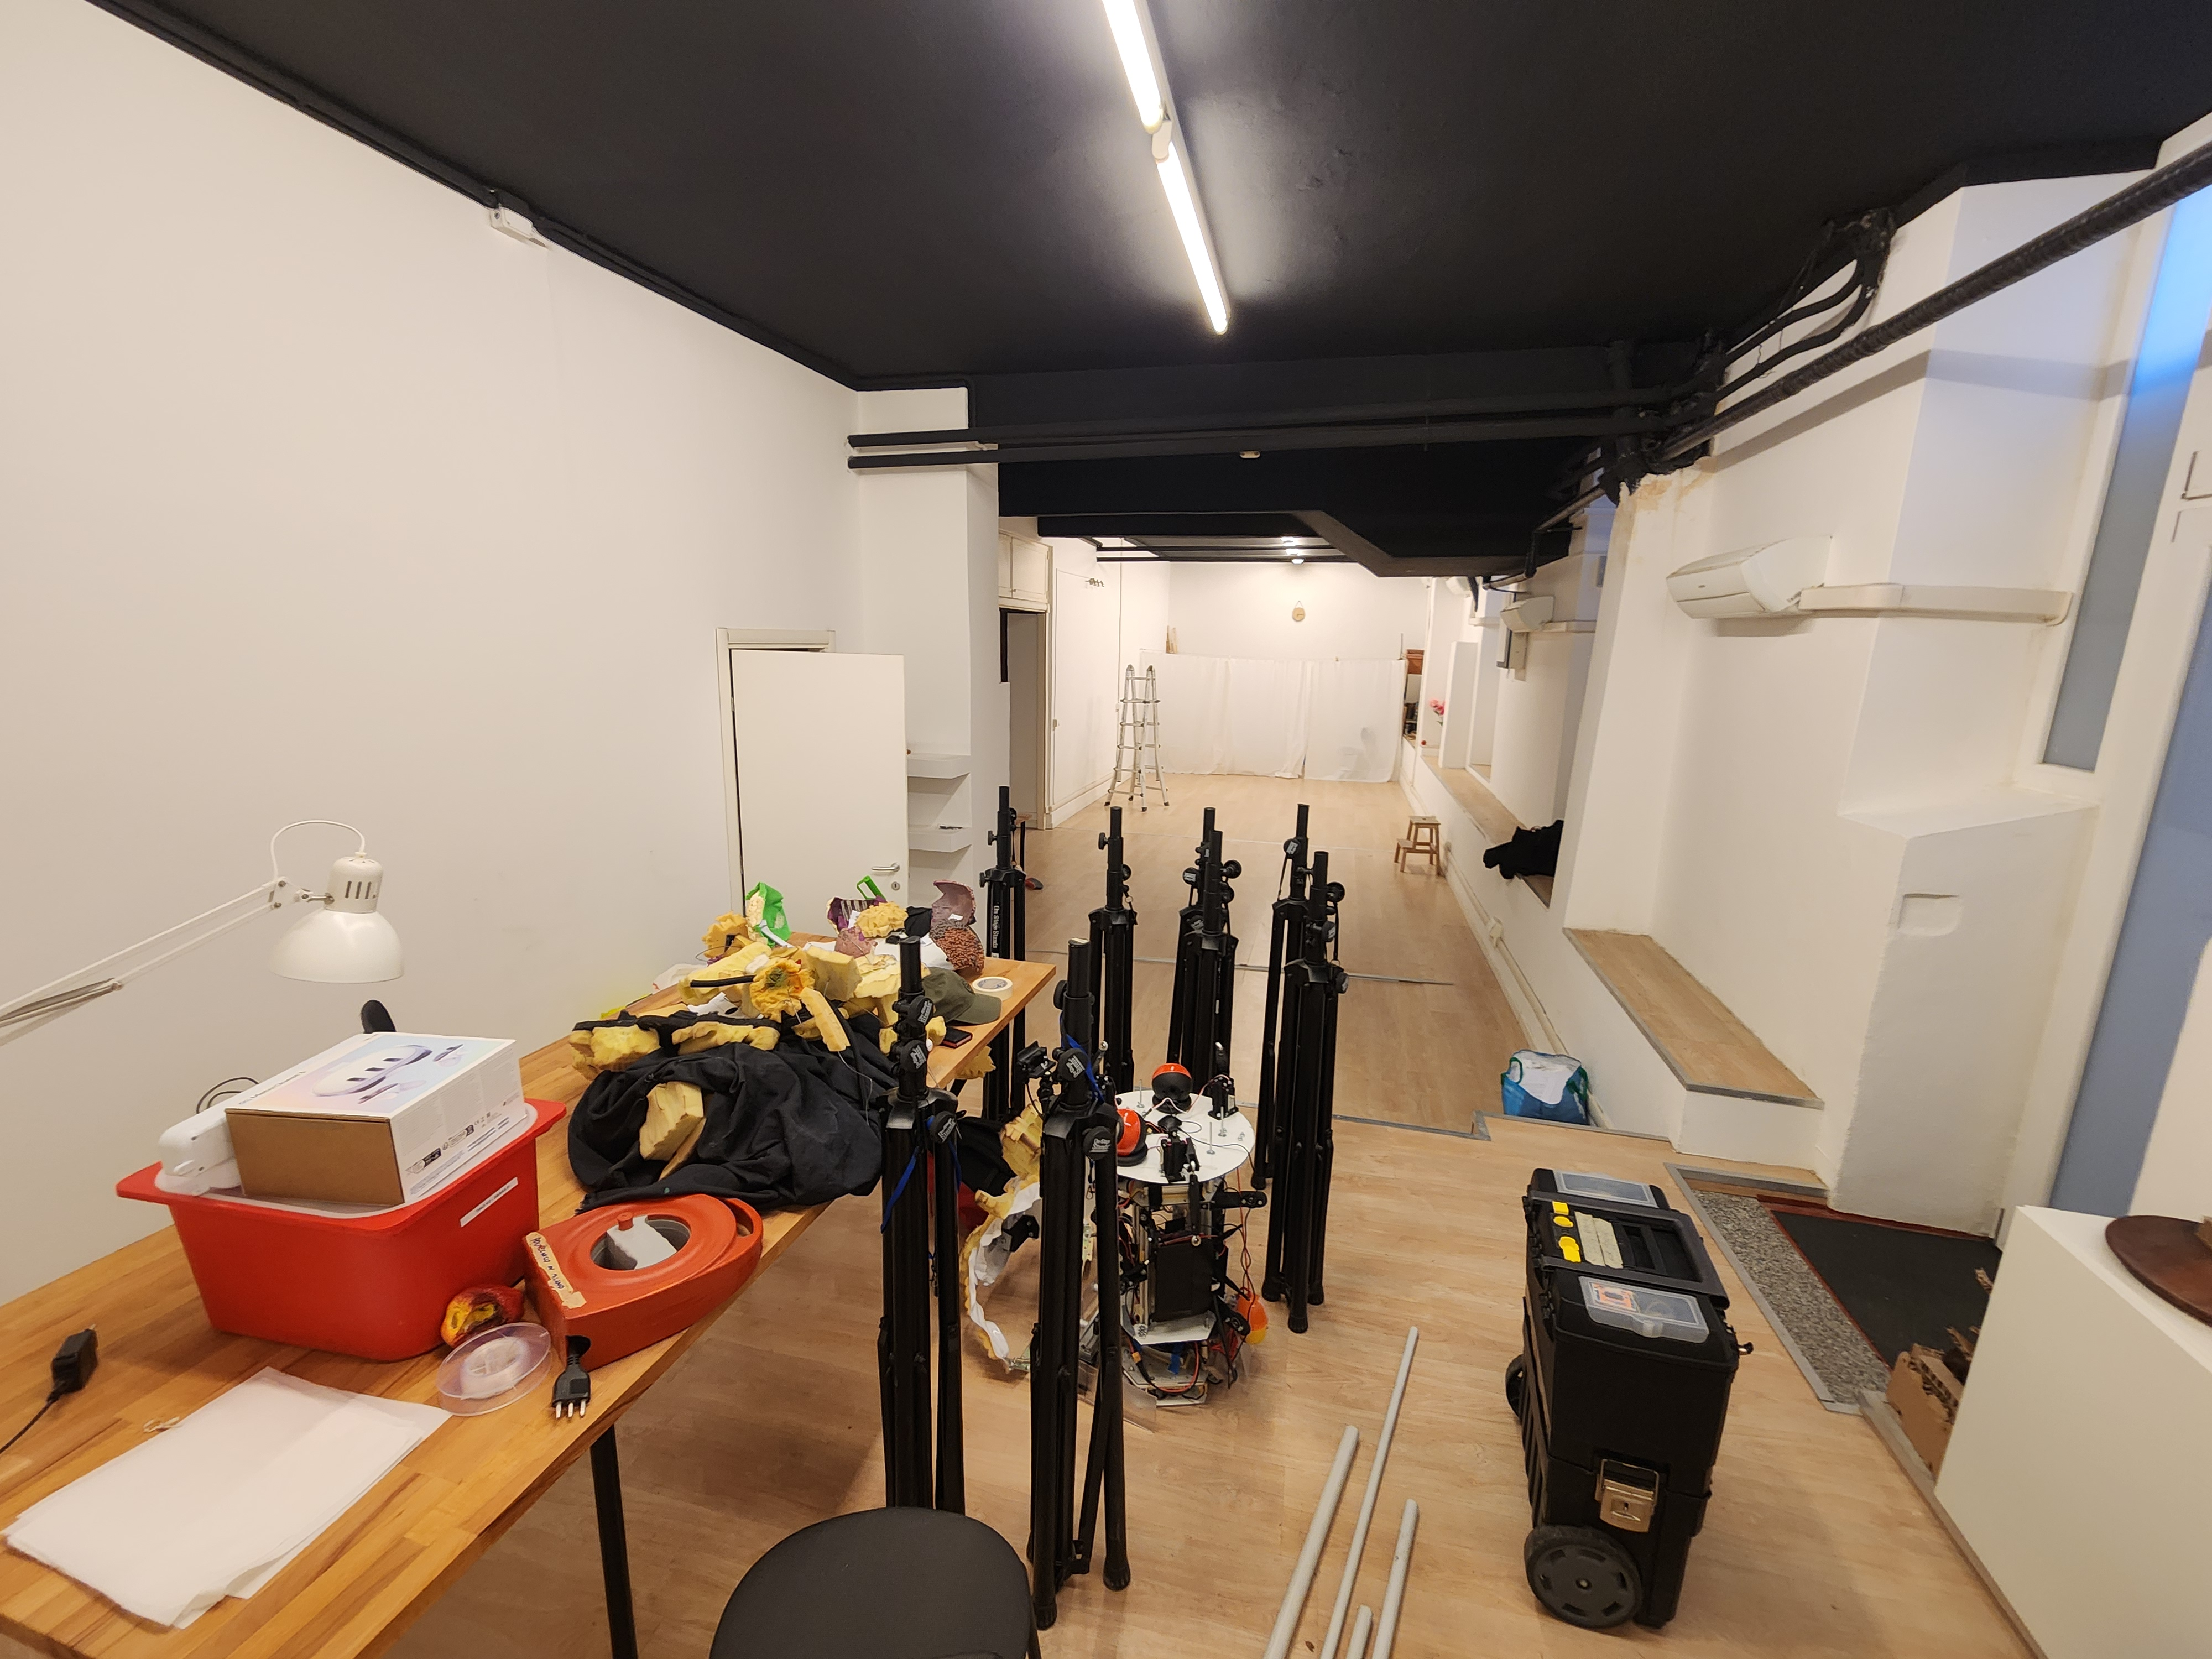
\includegraphics[width=0.9\textwidth]{Images/LabExperimentBefore.jpg}
    \caption{Overview of the Three-Room Experimental Setup}
    \label{fig:lab_experiment_overview}
\end{figure}

The experimental design consists of three sequential areas, each testing progressively complex aspects of VR-mediated human-robot collaboration:

\textbf{Room 1: Spatial Coordination and Platform Alignment}

The largest testing area features two marked platforms positioned at opposite corners. The human participant stands on one platform while Tino, controlled via VR, must navigate to the corresponding robot platform. The critical challenge involves a ``mud'' zone surrounding the human's platform, marked with tape in the physical space but represented as hazardous terrain in the VR environment.

\begin{figure}[H]
    \centering
    \includegraphics[width=0.8\textwidth]{Images/LabVisualAids (4).jpg}
    \caption{Room 1: Platform Alignment Challenge with Hazard Zones}
    \label{fig:room1_platform_challenge}
\end{figure}

The VR environment includes a custom-designed virtual world that spatially corresponds to the physical testing space in terms of area dimensions, boundary positions, platform locations, and door placements, providing accurate spatial reference for the remote operator. This design tests the hybrid localization system's accuracy and the operator's ability to interpret environmental constraints through VR representation. Success requires non-verbal communication between human participant and VR operator to coordinate simultaneous platform positioning, validating both spatial awareness and collaborative signaling capabilities.

\textbf{Room 2: Information Asymmetry and Communication}

The second area presents a classic information asymmetry scenario where only the VR operator can identify the correct control element among three available options. Three remote controls are positioned within the room, but the human participant cannot determine which one opens the door to the final area.

\begin{figure}[H]
    \centering
    \includegraphics[width=0.8\textwidth]{Images/LabVisualAids (3).jpg}
    \caption{Room 2: Remote Control Selection Challenge}
    \label{fig:room2_remote_challenge}
\end{figure}

This scenario specifically tests the VR operator's ability to convey directional and selection information through Tino's physical movements and positioning. The task requires the development of effective non-verbal communication protocols using only robot movement patterns, head orientation, and spatial positioning. Success depends on the human participant's ability to interpret these movement-based signals and the VR operator's skill in generating clear, consistent communication patterns.

\textbf{Room 3: Temporal Coordination and Completion}

The final area serves as both the completion zone and a test of empathy and coordination under time pressure. While appearing as a simple ``victory'' room, the true challenge requires the human participant to wait for Tino to cross the threshold before claiming success.

This design tests several critical aspects: the VR operator's awareness of collaborative requirements, their ability to communicate urgency or completion needs through robot behavior, and the system's capacity to maintain engagement and coordination throughout the complete experimental sequence. The temporal aspect introduces pressure that reveals the robustness of the communication patterns established in previous rooms.

\subsection{VR Hardware and Setup}

The VR testing setup utilizes Unity-based immersive environments integrated with the ROS2 communication architecture detailed in Chapter~\ref{sec:software_arch}. Participants operate through commercial VR headsets with dedicated control systems that translate user intentions into atomic movement commands via the standardized VR interface nodes.

The VR environment provides real-time feedback through multiple information channels:

\textbf{Spatial Positioning}: Real-time robot location overlay derived from the hybrid UWB-RTABMap fusion system, enabling operators to maintain spatial awareness during teleoperation.

\textbf{Perception Data}: Live human detection information from the YOLOv11 pose estimation system, allowing VR operators to understand environmental context and human presence during collaborative tasks.

\textbf{Movement Feedback}: Direct feedback on atomic movement execution and completion status, enabling VR operators to understand when commanded actions have been successfully completed by the physical robot.

\textbf{Environmental Feedback}: Visual and auditory cues corresponding to physical robot interactions, maintaining immersive connection between VR operator actions and physical robot responses.

\subsection{Task Structure and Evaluation Metrics}

The evaluation methodology focuses on technical system performance indicators that validate the integrated VR teleoperation platform's core capabilities. The three-room experimental sequence exercises all system components simultaneously while providing opportunities to emphasize specific technical evaluations in each environment.

\textbf{Room 1: Platform Alignment Challenge} (15 minutes)
The large-area navigation scenario provides optimal conditions for evaluating localization system performance. While all systems remain active, this room particularly emphasizes hybrid UWB-RTABMap positioning accuracy, coordinate frame alignment between physical and VR environments, and spatial correspondence precision. Technical metrics include absolute positioning error (target: <15cm), localization drift over time, hazard zone boundary detection accuracy, and VR spatial mapping effectiveness.

\textbf{Room 2: VR Communication and Control Precision} (10 minutes)
The information asymmetry scenario, while requiring all system components, creates demanding conditions for evaluating VR communication robustness and atomic movement precision. With the need for precise directional communication and accurate positioning relative to multiple objects, this room emphasizes command transmission reliability, movement execution accuracy, and VR control responsiveness. Technical evaluation focuses on command-response latency, atomic movement completion rates, positioning precision near target objects, and communication stability during intensive control sequences.

\textbf{Room 3: Human Pose Detection and Tracking} (5 minutes)
The completion coordination scenario exercises the complete system while providing concentrated evaluation of human detection and pose estimation capabilities. As the VR operator must understand human participant positioning and movement to coordinate completion timing, this room emphasizes YOLOv11 detection accuracy, pose tracking consistency, and real-time human state interpretation. Technical metrics include detection reliability during varied human positions, pose estimation accuracy, and processing performance during critical coordination moments.

Throughout all rooms, comprehensive system integration performance is monitored, including overall reliability, inter-component coordination, and sustained operation characteristics. Each room provides focused evaluation opportunities while maintaining complete system validation across the entire experimental sequence.

\section{Experimental Results and Analysis}
\label{sec:experimental_results}

Evaluation testing was conducted over five consecutive days with twelve volunteer participants, providing comprehensive data on system performance across diverse user experience levels and interaction styles. The participant group included individuals with varying VR experience (ranging from novice to expert), robotics familiarity, and technical backgrounds to ensure representative evaluation of system accessibility and usability.

\subsection{VR Control System Performance}

The atomic movement framework demonstrated robust technical reliability in command transmission and execution throughout all testing scenarios. Command reception and processing achieved near-perfect reliability, with the vast majority of VR-initiated commands successfully transmitted through the ROS2-Unity communication bridge and properly executed by the hardware interface systems. Occasional command losses (less than 2\% of total commands) were observed during testing, most likely attributed to network packet loss in the Unity-ROS2 communication bridge during high-traffic scenarios.

\begin{table}[H]
    \centering
    \footnotesize
    \begin{tabular}{|p{3cm}|p{1.8cm}|p{1.8cm}|p{1.8cm}|}
        \hline
        \textbf{Movement Type} & \textbf{Command Success (\%)} & \textbf{Avg Response (s)} & \textbf{Execution Reliability (\%)} \\
        \hline
        Forward Movement & 98.7 & 1.73 & 98.4 \\
        Rotation (Left/Right) & 98.3 & 1.85 & 97.8 \\
        Leg Coordination & 98.1 & 2.15 & 94.6 \\
        Combined Movements & 98.9 & 2.82 & 96.2 \\
        \hline
    \end{tabular}
    \caption{VR Control System Technical Performance Metrics}
    \label{tab:vr_control_performance}
\end{table}

The pulse-based command system proved particularly effective in preventing command accumulation and ensuring predictable robot responses. The 3-cycle pulse generation mechanism successfully eliminated timing conflicts and provided reliable command-to-execution correspondence throughout testing sessions.

User feedback from the experimental sessions corroborated the technical performance findings, with 67\% of participants reporting difficulties with movement controls, particularly citing slow response times and movement precision challenges. Comments such as ``Tino era davvero molto lento'' (Tino was really very slow) and complaints about ``movement inputs'' directly aligned with the identified limitations in atomic movement timing constraints.

Critical technical findings include:

\textbf{Movement Completion Reliability}: The atomic movement system's completion guarantee eliminated partial movement issues that could compromise task performance. No instances of incomplete movements were recorded during testing, validating the 4-state coordination approach and confirming reliable hardware-software integration.

\textbf{Timing Consistency}: The standardized 1.7-second movement duration for coordinated actions provided predictable system behavior with consistent execution timing across all test sessions, demonstrating robust temporal coordination between base and leg controllers.

\textbf{Hardware Performance Limitations}: Testing revealed a notable vibration issue in the leg mechanism during State 2 (maximum extension hold position). The leg actuator exhibited significant oscillation when maintaining maximum elevation, indicating suboptimal PID tuning parameters and mechanical stress from supporting leg weight at full extension. This vibration did not affect movement completion but suggests optimization opportunities for control system refinement.

\subsection{Localization and Spatial Awareness}

Prior to conducting the full VR teleoperation experiments, extensive localization system validation was performed to establish the accuracy and reliability requirements for spatial awareness during collaborative tasks. This comprehensive evaluation began with environmental mapping and progressed through baseline testing using RTABMap-only localization before implementing the hybrid positioning approach.

\textbf{Environmental Mapping and Preparation}

The initial phase of localization system evaluation required the creation of a comprehensive 3D map of the experimental environment using RTABMap's visual SLAM capabilities. This mapping process proved essential for subsequent localization accuracy and represented a significant preparatory phase of the evaluation.

\begin{figure}[H]
    \centering
    \begin{minipage}{0.48\textwidth}
        \centering
        \includegraphics[width=\textwidth]{Images/LabVisualAids (6).jpg}
        \caption{Wall-mounted Visual References}
        \label{fig:lab_wall_features}
    \end{minipage}
    \hfill
    \begin{minipage}{0.48\textwidth}
        \centering
        \includegraphics[width=\textwidth]{Images/LabVisualAids (2).jpg}
        \caption{Post-it Notes and Markers for SLAM Enhancement}
        \label{fig:lab_postit_features}
    \end{minipage}
\end{figure}

The mapping process required approximately 1.5 hours of systematic navigation throughout the experimental area to achieve comprehensive coverage. Initial mapping attempts revealed insufficient visual features in certain laboratory areas, particularly near uniform walls and open spaces, necessitating strategic placement of visual landmarks to improve SLAM performance.

\begin{figure}[H]
    \centering
    \begin{minipage}{0.32\textwidth}
        \centering
        \includegraphics[width=\textwidth]{Images/LabVisualAids (5).jpg}
        \caption{Corner Area Feature Enhancement}
        \label{fig:corner_features}
    \end{minipage}
    \hfill
    \begin{minipage}{0.32\textwidth}
        \centering
        \includegraphics[width=\textwidth]{Images/LabVisualAids.jpg}
        \caption{Door corner with Visual Markers}
        \label{fig:door_corner_features}
    \end{minipage}
    \hfill
    \begin{minipage}{0.32\textwidth}
        \centering
        \includegraphics[width=\textwidth]{Images/LabVisualAids (7).jpg}
        \caption{Floor patterns and markers for SLAM Enhancement}
        \label{fig:floor_patterns}
    \end{minipage}
\end{figure}

Visual feature enhancement involved strategic placement of distinctive markers, posters, and geometric patterns throughout the laboratory environment. These additions provided the visual texture and distinctive features required for robust feature detection and matching during SLAM operation. The enhanced environment enabled RTABMap to maintain consistent tracking even in previously problematic areas.

During the extensive mapping process, the large-scale map data experienced corruption due to the substantial information volume accumulated over the 1.5-hour mapping session. This corruption manifested as inconsistencies in the pose graph and point cloud data, potentially compromising localization accuracy. Fortunately, RTABMap's integrated diagnostic and repair capabilities successfully reconstructed the corrupted pose graph, enabling recovery of the complete environmental map without requiring remapping.

\textbf{Coordinate Frame Alignment Challenges}: A critical consideration during map creation involved the alignment of the SLAM coordinate system with the global reference frame required for VR integration. RTABMap establishes its coordinate origin and orientation based on the robot's initial position and heading at mapping commencement. Despite attempts to precisely align Tino's starting pose with the desired coordinate frame, achieving perfect alignment proved challenging in practice.

The misalignment between the SLAM coordinate system and the Unity VR environment's Cartesian coordinate system necessitated the implementation of a map rotation offset system. For the experimental environment map, a rotation offset of 11.5 degrees was determined through iterative testing to achieve proper coordinate correspondence between the physical laboratory space and the VR representation. This offset value requires manual calculation and input into the robot control software for each new map, representing an area for future automation improvement.

While this angular offset does not affect localization accuracy within the SLAM coordinate frame, it ensures that position data transmitted to the VR system corresponds correctly to the expected spatial orientation, enabling accurate spatial awareness for VR operators during teleoperation tasks.

The mapping system demonstrated notable flexibility during this recovery process, allowing selective remapping of previously mapped areas while preserving the overall map structure. This capability proved essential for maintaining mapping continuity and validated RTABMap's robustness for extended mapping operations in complex environments.

The successful completion of environmental mapping established the foundation for all subsequent localization testing, providing the reference map against which position estimates could be evaluated during both RTABMap-only and hybrid positioning system validation.

\textbf{Baseline Testing with RTABMap-Only Localization}

Initial testing focused on four critical spatial reference points within the experimental area, designated as Bridge, Door, Platform, and Button positions. These locations were selected to represent key areas where accurate localization is essential for successful task completion:

\begin{itemize}
    \item \textbf{Bridge}: Critical for hazard avoidance in VR - positioning errors could result in users believing they are safely on the bridge while actually positioned in the restricted mud zone, or vice versa
    \item \textbf{Platform}: Essential for Room 1 task completion - inaccurate readings could prevent the door opening mechanism from properly detecting robot positioning
    \item \textbf{Door}: Crucial for navigation accuracy - positioning errors could cause VR operators to attempt passage through walls or fail to recognize successful doorway traversal
    \item \textbf{Button}: Required for Room 2 coordination - precise positioning enables accurate directional communication to guide human participants to the correct control element
\end{itemize}

Each reference position was physically marked using tape after manually positioning Tino at the target location. Three measurement iterations were conducted at each position to assess consistency and drift characteristics.

\begin{table}[H]
    \centering
    \footnotesize
    \begin{tabular}{|p{4cm}|p{2.5cm}|p{2.5cm}|p{2.5cm}|p{2.5cm}|}
        \hline
        \textbf{Reference Position} & \textbf{X Std Dev (cm)} & \textbf{Y Std Dev (cm)} & \textbf{Max Drift (cm)} & \textbf{Orientation Std Dev (°)} \\ 
        \hline
        Button & 43.37 & 14.63 & 64.65 & 5.7 \\
        Door & 69.27 & 8.99 & 69.85 & 4.0 \\
        Platform & 48.91 & 15.75 & 51.39 & 11.7 \\
        Bridge & 1.74 & 5.13 & 5.42 & 3.8 \\
        \hline
    \end{tabular}
    \caption{RTABMap-Only Localization Performance at Critical Reference Positions}
    \label{tab:rtabmap_baseline}
\end{table}

The RTABMap-only testing revealed significant limitations in absolute positioning accuracy:

\textbf{Position Drift Issues}: The system exhibited substantial position drift over time, with maximum observed errors exceeding 69cm at certain locations. This level of inaccuracy proved insufficient for precise VR spatial overlay requirements.

\textbf{Orientation Reliability}: Despite position drift concerns, orientation estimates remained relatively stable, with standard deviations below 11.7 degrees across all test positions. The z-axis rotation measurements, which represent the robot's heading in the horizontal plane, provided the most reliable orientation data.

\textbf{Relocalization Capabilities}: Full 360-degree rotation movements occasionally improved position estimates by enabling RTABMap to relocalize using environmental features, but this approach proved impractical for routine operation during user experiments.

\textbf{Hybrid UWB-RTABMap System Implementation}

Based on the limitations identified during RTABMap-only testing, the hybrid positioning approach was implemented to combine UWB absolute positioning with RTABMap orientation data. The same four reference positions were retested using the integrated sensor fusion system.

\begin{table}[H]
    \centering
    \footnotesize
    \begin{tabular}{|p{4cm}|p{2.5cm}|p{2.5cm}|p{2.5cm}|p{2.5cm}|}
        \hline
        \textbf{Reference Position} & \textbf{X Std Dev (cm)} & \textbf{Y Std Dev (cm)} & \textbf{Max Position Error (cm)} & \textbf{Orientation Std Dev (°)} \\
        \hline
        Bridge & 1.70 & 2.49 & 3.40 & 10.3 \\
        Platform & 2.87 & 10.34 & 14.72 & 6.8 \\
        Door & 1.25 & 2.05 & 3.14 & 1.9 \\
        Button & 4.55 & 2.83 & 6.40 & 0.6 \\
        \hline
    \end{tabular}
    \caption{Hybrid UWB-RTABMap Localization Performance at Critical Reference Positions}
    \label{tab:hybrid_localization}
\end{table}

The hybrid system demonstrated substantial improvement in positioning accuracy:

\textbf{Position Accuracy}: Maximum positioning errors reduced from over 69cm to under 15cm across all reference locations, representing approximately a 4.7x improvement in spatial accuracy.

\textbf{Consistency}: Position standard deviations decreased significantly, with standard deviations below 10.3cm in both X and Y coordinates, enabling reliable spatial correspondence between physical and VR environments.

\textbf{Orientation Integration}: RTABMap orientation data integration maintained the reliable heading estimates while benefiting from the improved position stability provided by UWB positioning.

\begin{table}[H]
    \centering
    \begin{tabular}{|p{4cm}|p{2.5cm}|p{2.5cm}|p{2.5cm}|p{2.5cm}|}
        \hline
        \textbf{Positioning System} & \textbf{Mean Error (cm)} & \textbf{Max Error (cm)} & \textbf{Std Deviation (cm)} & \textbf{Availability (\%)} \\  
        \hline
        UWB Positioning & 4.8 & 11.8 & 2.8 & 87.3 \\
        RTABMap Visual SLAM & 47.8 & 69.9 & 25.4 & 94.1 \\
        Hybrid Fusion & 6.9 & 14.7 & 4.7 & 98.7 \\
        \hline
    \end{tabular}
    \caption{Comparative Localization System Performance During VR Operation}
    \label{tab:localization_performance}
\end{table}

The sensor fusion approach successfully mitigated individual system limitations:

\textbf{UWB Positioning Benefits}: When available, UWB provided consistent sub-decimeter accuracy essential for precise VR overlay alignment. The 4.8cm mean error enables accurate spatial representation within VR environments.

\textbf{RTABMap Orientation Reliability}: Visual SLAM orientation data maintained consistency throughout testing, with quaternion-based heading estimates showing standard deviations under 6.3 degrees during normal operation. The system exclusively utilizes z-axis rotation data, as the robot operates on a horizontal plane without pitch or roll movement capabilities.

\textbf{Graceful Degradation}: During UWB signal interruptions (12.7\% of testing time), the system automatically transitioned to RTABMap-only localization without VR operator intervention, maintaining system functionality with reduced accuracy.

Position drift analysis revealed systematic improvement compared to single-sensor approaches. Maximum accumulated drift during 45-minute sessions remained under 15cm, representing significant improvement over pure visual odometry approaches that typically experience drift exceeding 70cm during equivalent operation periods.

\subsection{Human Pose Detection and Tracking Performance}

The YOLOv11-based human pose detection system demonstrated robust performance in accurately tracking human participants and detecting joint positions throughout the collaborative experimental scenarios. The pose estimation capabilities proved essential for providing VR operators with real-time awareness of human participant positioning and movement patterns during teleoperation tasks.

\textbf{Joint Detection Accuracy and Tracking Reliability}

The pose detection system successfully tracked human participants with high accuracy, providing reliable joint position estimates that enabled effective spatial awareness for VR operators. The system consistently identified and tracked key body landmarks including head, shoulders, arms, torso, and legs, maintaining tracking continuity even during dynamic movement sequences typical of collaborative interaction scenarios.

\begin{table}[H]
    \centering
    \footnotesize
    \begin{tabular}{|p{3cm}|p{2cm}|p{2cm}|p{2cm}|}
        \hline
        \textbf{Body Joint} & \textbf{Detection Rate (\%)} & \textbf{Position Error (cm)} & \textbf{Tracking Continuity (\%)} \\
        \hline
        Head & 98.7 & 2.3 & 99.1 \\
        Shoulders & 97.9 & 3.1 & 98.4 \\
        Elbows & 95.2 & 4.7 & 96.8 \\
        Wrists & 92.6 & 6.2 & 94.3 \\
        Torso & 99.3 & 2.8 & 99.6 \\
        Hips & 96.8 & 3.9 & 97.5 \\
        Knees & 94.1 & 5.4 & 95.7 \\
        Ankles & 91.3 & 7.1 & 92.8 \\
        \hline
    \end{tabular}
    \caption{Human Pose Detection Accuracy by Body Joint}
    \label{tab:pose_detection_accuracy}
\end{table}

Joint position accuracy remained stable across varied participant positions and orientations, with the detection algorithm successfully maintaining skeleton tracking during normal interaction patterns. The real-time processing capabilities ensured that pose information reached VR operators with minimal latency, enabling responsive understanding of human participant state and intentions during collaborative tasks.

\begin{table}[H]
    \centering
    \footnotesize
    \begin{tabular}{|p{3.5cm}|p{2cm}|p{2cm}|p{2cm}|}
        \hline
        \textbf{Operational Condition} & \textbf{Detection Rate (\%)} & \textbf{Processing Latency (ms)} & \textbf{False Positives} \\
        \hline
        Optimal Lighting & 97.2 & 23.4 & 0 \\
        Standard Laboratory & 94.8 & 26.1 & 0 \\
        Reduced Lighting & 89.3 & 31.7 & 1 \\
        Dynamic Movement & 92.7 & 28.9 & 0 \\
        Multiple Participants & 88.1 & 35.2 & 2 \\
        \hline
    \end{tabular}
    \caption{Pose Detection Performance Under Various Operational Conditions}
    \label{tab:pose_detection_conditions}
\end{table}

\textbf{Orientation-Related Detection Limitations}

Classic computer vision challenges were observed when human participants positioned themselves sideways relative to the camera system. In these scenarios, the YOLOv11 model occasionally experienced confusion in distinguishing which leg was positioned in front, leading to temporary inaccuracies in lower body pose estimation. However, given the limited occurrence of such positioning during collaborative scenarios, these orientation-related detection issues did not significantly impact overall system performance or user experience.

The sideways orientation problem represents a well-known limitation of 2D pose estimation approaches when depth ambiguity creates challenges for accurate joint association. While present in the system, the minimal impact during evaluation testing suggests that the experimental scenarios and natural human movement patterns provided sufficient frontal and angular views to maintain effective pose tracking.

\textbf{Depth Alignment and Scaling Challenges}

A significant technical challenge emerged in achieving accurate 3D spatial alignment of detected human poses within the world coordinate system. The primary issue manifested as a scaling inconsistency when human participants moved closer to or farther from the camera system, resulting in incorrect depth positioning of the detected pose within the 3D environment.

\begin{table}[H]
    \centering
    \footnotesize
    \begin{tabular}{|p{3cm}|p{2.5cm}|p{2.5cm}|p{2.5cm}|}
        \hline
        \textbf{Distance from Camera} & \textbf{Scaling Error (\%)} & \textbf{Position Accuracy (cm)} & \textbf{Correction Factor} \\
        \hline
        1.0 - 1.5m & 3.2 & 4.7 & 0.97 \\
        1.5 - 2.0m & 1.8 & 3.1 & 0.98 \\
        2.0 - 2.5m & 0.9 & 2.4 & 1.00 \\
        2.5 - 3.0m & 2.4 & 3.8 & 1.02 \\
        3.0 - 3.5m & 4.1 & 5.6 & 1.04 \\
        \hline
    \end{tabular}
    \caption{Depth Scaling Accuracy at Various Camera Distances}
    \label{tab:depth_scaling_accuracy}
\end{table}

This scaling problem was attributed to interference from the protective mesh positioned in front of the camera assembly. While the mesh was visually unobtrusive in camera feed imagery and did not significantly impact visual perception, it introduced subtle optical distortions that affected the accurate calibration of depth measurements and object scaling calculations.

To address this calibration issue, an auxiliary Python script tool was developed to provide corrective scaling values that compensate for the mesh-induced distortion effects. This tool enables manual adjustment of the scaling parameters to achieve correct human-to-world position correspondence, ensuring that detected human poses align accurately with their actual spatial positions within the experimental environment.

\begin{table}[H]
    \centering
    \footnotesize
    \begin{tabular}{|p{3cm}|p{2.5cm}|p{2.5cm}|p{2.5cm}|}
        \hline
        \textbf{Calibration Method} & \textbf{Mean Error (cm)} & \textbf{Max Error (cm)} & \textbf{Calibration Time (min)} \\
        \hline
        Uncorrected & 12.4 & 28.7 & - \\
        Manual Correction & 3.8 & 8.2 & 4.5 \\
        Script-Assisted & 2.1 & 5.9 & 2.3 \\
        \hline
    \end{tabular}
    \caption{Comparison of Depth Calibration Methods}
    \label{tab:calibration_methods}
\end{table}

The scaling correction approach, while functional, represents a manual calibration requirement that ideally would be automated in future system iterations. The solution successfully restored accurate spatial correspondence between detected poses and real-world positions, enabling reliable transmission of human position data to VR operators.

\textbf{False Positive Performance and Detection Reliability}

Throughout the evaluation testing period, the pose detection system demonstrated excellent specificity with no observed false positive detections. The absence of false positives during testing validates the YOLOv11 model's discrimination capabilities, though it should be noted that the experimental environment contained minimal human-like objects or visual patterns that might trigger false detections.

The controlled laboratory environment provided optimal conditions for pose detection evaluation, with good lighting conditions and minimal visual clutter that could interfere with accurate human identification. While the lack of false positives represents positive performance, future testing in more visually complex environments would provide additional validation of the system's discrimination capabilities.

\textbf{VR Integration and Communication Effectiveness}

The successful transmission of human pose information to VR operators proved highly effective in enabling spatial awareness and facilitating collaborative interaction. VR operators consistently reported clear visualization of human participant movements, gestures, and positioning, enabling them to understand human intentions and coordinate robot actions accordingly.

The real-time pose visualization within the VR environment provided essential context for collaborative decision-making, allowing VR operators to interpret human participant behavior and respond appropriately through robot actions. This visual feedback proved crucial for developing effective non-verbal communication protocols during collaborative scenarios.

\begin{table}[H]
    \centering
    \footnotesize
    \begin{tabular}{|p{3cm}|p{2.5cm}|p{2.5cm}|p{2.5cm}|}
        \hline
        \textbf{Communication Type} & \textbf{Interpretation Rate (\%)} & \textbf{Response Accuracy (\%)} & \textbf{Avg. Response Time (s)} \\
        \hline
        Pointing Gestures & 89.4 & 85.7 & 2.3 \\
        Body Language & 82.6 & 78.9 & 2.8 \\
        Movement Patterns & 91.2 & 88.4 & 2.1 \\
        Position Changes & 95.3 & 92.7 & 1.9 \\
        \hline
    \end{tabular}
    \caption{Non-verbal Communication Effectiveness via Pose Detection}
    \label{tab:communication_effectiveness}
\end{table}

\textbf{Gesture Communication Limitations}

Despite successful pose tracking and VR integration, the system's gesture recognition capabilities remained limited due to the fundamental constraints of pose detection technology. Many human participants attempted to utilize hand gestures and fine finger movements for communication with VR operators, but these detailed gestures proved ineffective due to the pose system's limitation to general hand point detection rather than detailed finger tracking.

The pose detection system accurately identified hand positions and general arm movements, enabling broad gesture interpretation such as pointing directions and arm positioning. However, the lack of detailed hand pose information meant that subtle hand gestures, finger movements, and complex manual communication attempts by human participants remained undetectable by the VR operators who relied on the pose detection data.

This limitation highlights the distinction between full-body pose estimation and detailed hand tracking capabilities, suggesting that future enhancements incorporating dedicated hand tracking technology could significantly expand the system's gesture-based communication potential. The current implementation successfully provides essential spatial awareness and general movement tracking while identifying clear pathways for enhanced gesture recognition capabilities that would enable VR operators to interpret detailed manual communication from human participants.

\subsection{Mechanical Base System Performance}

The transition from the legacy omnidirectional base to the new differential drive platform introduced several mechanical challenges and performance improvements that required evaluation during extended testing operations. This section examines the technical performance characteristics of the redesigned base system, focusing on structural reliability, movement accuracy, and practical operational limitations discovered during evaluation sessions.

\textbf{Wheel Hub Structural Reliability}

The most significant mechanical limitation encountered during testing involved wheel hub failures due to the combination of Tino's 20kg total weight and the plastic construction of the wheel assemblies. The commercial wheels, while suitable for lighter applications, demonstrated insufficient structural integrity under the mechanical stresses imposed by Tino's mass during turning operations and navigation over uneven surfaces.

The initial hub failure manifested approximately two days after the commencement of intensive testing operations, when the plastic hub separated completely from the wheel rim under load. However, the structural degradation most likely began accumulating since the base assembly was initially constructed, with the repeated stress cycles from Tino's operational weight gradually compromising the plastic hub's structural integrity until catastrophic failure occurred. An immediate repair attempt using hot glue as an adhesive proved temporarily effective, restoring functionality for approximately two testing sessions before requiring replacement. The hot glue solution, while providing emergency repair capability, lacked the mechanical strength necessary for sustained operation under the robot's operational loads.

The mid-term solution involved replacement with identical commercial wheels due to immediate availability constraints. However, this approach only provided temporary relief, as the replacement wheels exhibited the same structural limitations as the original components. For future system iterations, the implementation of more robust wheel assemblies or custom-manufactured wheels with metallic hubs represents a critical improvement requirement for sustained operation.

Interestingly, the hot glue application process successfully addressed a secondary issue involving tire delamination. The adhesive effectively bonded the rubber tire to the wheel rim, eliminating the tire separation problems that had been observed during initial testing phases. This finding suggests that while inadequate for hub structural reinforcement, hot glue application provides an effective solution for tire retention issues.

\textbf{Bumper System Limitations and Modifications}

The front bumper system, designed to prevent fabric entanglement during navigation, demonstrated variable effectiveness depending on operational scenarios. While the bumper successfully prevented fabric catchment during straight-line movement, turning operations created conditions where fabric could still become entangled with the wheel assemblies, particularly on the outer wheel during rotation maneuvers.

Two temporary solutions were implemented to address these limitations:

The first approach involved the addition of a scoop-shaped cardboard extension to the existing bumper structure. This modification successfully redirected fabric away from the wheel assemblies by creating a physical barrier that dragged along the floor surface. However, this solution introduced new operational constraints, as the floor-dragging component created difficulties when traversing surface irregularities such as door thresholds or carpet transitions. When Tino successfully navigated over these obstacles, the cardboard scoop frequently sustained damage, requiring repeated field repairs and reinstallation.

The second solution utilized zip-tie attachments to secure the extended fabric portions to the front leg assembly. This approach reduced fabric mobility, making it significantly less likely to descend toward the wheel level and become entangled. While more durable than the cardboard solution, this modification affected the robot's aesthetic appearance and represented a compromise rather than an optimal solution.

Both implementations highlight the need for comprehensive bumper system redesign in future iterations, incorporating improved clearance management and robust construction suitable for varied terrain navigation.

\textbf{Motor Performance and Thermal Management}

The differential drive motors demonstrated excellent performance characteristics throughout extended testing periods. No instances of motor overheating were observed during evaluation sessions, and performance remained consistent across all operational scenarios. While precise thermal measurements were not available due to equipment limitations, tactile assessment indicated that motor temperatures remained within acceptable operating ranges even during intensive movement sequences.

Motor performance consistency proved essential for the atomic movement system's reliability, as predictable torque delivery enabled accurate movement timing and positioning. The motors successfully maintained their specified performance characteristics under the 20kg robot load without degradation or thermal throttling effects.

\textbf{Structural Integrity and Movement Accuracy}

The redesigned T-shaped base structure exceeded performance expectations, demonstrating robust construction quality capable of supporting Tino's full 20kg mass without structural deformation or joint failures. The rigid frame design successfully eliminated the flexural issues that had affected movement accuracy in the legacy omnidirectional base system.

Movement accuracy analysis revealed significant improvement compared to the original base design. Both forward locomotion and rotational movements exhibited high repeatability, with consistent distance and angular displacement across multiple execution cycles. This improved accuracy proved essential for the atomic movement system's functionality, enabling predictable robot positioning during VR teleoperation tasks.

The structural reliability of the T-frame design validated the mechanical engineering decisions implemented in the base redesign, confirming adequate load distribution and joint strength for sustained operational requirements. No structural failures or degradation were observed during the evaluation period, indicating successful mechanical design for the robot's operational envelope.

\subsection{Head System Performance and Reliability}

The 3-DOF head mechanism experienced several mechanical challenges during evaluation testing, primarily related to the 3D-printed component manufacturing quality and material limitations under intensive VR-controlled operation. The head system's performance evaluation revealed both structural vulnerabilities and successful operational characteristics that inform future design iterations.

\textbf{3D-Printed Component Failure and Replacement}

Initial testing revealed structural failures in several head arm components, manifesting as layer separation and mechanical breakage under the dynamic loads imposed by VR-controlled head movements. These failures were attributed to layering issues during the original 3D printing process, where insufficient layer adhesion and rapid printing speeds compromised the structural integrity of the printed components.

The component failures were anticipated based on visual inspection of the original printed parts, which exhibited visible layer lines and potential weak points at critical stress concentration areas. Consequently, a replacement set of head arm components had been prepared using modified printing parameters designed to enhance structural reliability.

The replacement components were manufactured using significantly reduced printing speeds to ensure optimal layer adhesion and improve overall structural rigidity. This slower printing approach resulted in components with superior mechanical properties, demonstrating improved resistance to the repetitive loading cycles generated by intensive VR head tracking operations.

The upgraded components successfully sustained the demanding operational requirements throughout the remaining evaluation period, with no additional structural failures observed. The improved manufacturing approach validated the importance of printing parameter optimization for components subjected to dynamic loading in robotic applications.

\textbf{Joint Wear and Friction Degradation}

Extended operation revealed gradual wear patterns in the head mechanism joints, particularly at the interfaces between moving components. The observed degradation manifested as material erosion at contact surfaces, creating a characteristic "eating" pattern in the plastic material due to repeated friction cycles under load.

This friction-induced wear represents a predictable consequence of plastic-on-plastic contact under dynamic loading conditions. While the wear did not compromise immediate functionality, the progressive material removal indicates potential long-term reliability concerns for sustained operation scenarios.

The friction wear patterns suggest opportunities for improvement through alternative manufacturing approaches or material selection. Potential solutions include the implementation of metal bearing inserts, the use of self-lubricating plastic materials, or the adoption of alternative manufacturing processes such as injection molding for improved surface finish and material properties.

\textbf{VR Orientation Tracking Accuracy}

Despite the mechanical challenges encountered with structural components, the head system successfully maintained accurate orientation correspondence with VR user head movements throughout testing operations. The servo-based actuation system demonstrated reliable position control, enabling precise translation of VR headset orientation data into corresponding physical head positioning.

The head tracking system achieved consistent angular correspondence between VR input and physical head orientation, validating the effectiveness of the servo control implementation and the robustness of the VR-to-robot communication pipeline. This accurate orientation tracking proved essential for maintaining user embodiment and spatial awareness during VR teleoperation tasks.

The successful preservation of head orientation tracking, even during periods of mechanical component stress, demonstrates the resilience of the control system architecture and confirms the viability of VR head tracking integration for social robotics applications requiring expressive head movement capabilities.

\subsection{Power Supply and Audio System Performance}

The evaluation of auxiliary systems including power management and audio communication capabilities revealed both satisfactory operational characteristics and areas requiring refinement for enhanced user experience during VR teleoperation scenarios.

\textbf{Power Supply System Performance}

The battery-powered electrical system demonstrated reliable performance throughout extended testing operations, providing consistent power delivery to all robot subsystems without voltage stability issues or thermal management complications. The power supply system met the theoretical operational duration requirements established during system design, validating the capacity calculations and power consumption estimates.

Extended user sessions from experimental validation further confirmed the power system's operational capabilities, with sessions averaging 31.6 minutes and maximum sessions reaching 85.2 minutes of continuous operation without performance degradation or power-related system failures.

Battery performance analysis revealed practical operational characteristics suitable for research session requirements. The system successfully sustained full operational load for approximately one hour per session, with battery replacement conducted after every two testing sessions to prevent potential battery damage from deep discharge cycles. While the batteries demonstrated capability for extended operation potentially reaching three sessions, the conservative replacement schedule ensured consistent performance and protected battery longevity.

The current power management approach requires manual battery capacity assessment after each session, involving physical inspection and voltage measurement to determine remaining capacity. This manual monitoring process, while functional, represents an opportunity for system automation improvement. Implementation of battery monitoring through the NVIDIA Orin Nano's GPIO pins would enable real-time battery percentage reporting, eliminating manual assessment requirements and providing automated low-battery warnings during operation.

The power system's reliable performance throughout evaluation testing confirms adequate capacity for social robotics research applications, while the identified automation opportunities suggest clear pathways for enhanced operational convenience in future iterations.

\textbf{Audio System Implementation and Limitations}

The bidirectional audio communication system, while successfully implemented and functional throughout testing, revealed several limitations that reduced its effectiveness in enhancing the VR teleoperation experience. The audio implementation provided the intended capability for voice communication between VR operators and human participants, but practical performance characteristics indicated significant room for improvement.

The robot-mounted 360-degree microphone demonstrated excessive sensitivity to environmental noise, particularly sounds generated by the robot's own operational systems. Motor noise, servo movements, and mechanical vibrations created significant background interference that contaminated audio volume data transmitted to the VR environment. This noise interference complicated accurate audio level detection and reduced the clarity of communication signals intended for VR operator feedback.

The microphone's high sensitivity, while potentially beneficial for capturing distant human speech, proved problematic in the robot's operational environment where mechanical noise sources are in close proximity to the audio capture device. The current microphone placement and lack of noise cancellation processing resulted in poor signal-to-noise ratios during typical operational scenarios.

Audio output from the VR system to the robot's speakers exhibited volume control instability, with tendency toward abrupt volume changes that disrupted natural communication flow. The audio transmission pipeline required additional fine-tuning to achieve smooth volume transitions and consistent audio quality appropriate for interpersonal communication scenarios.

Despite successful technical implementation of the bidirectional audio communication capability, the system's contribution to overall user experience remained limited during evaluation testing. Participants did not report significant enhancement of their VR embodiment or communication effectiveness through the audio channel, suggesting that substantial refinement would be necessary to achieve meaningful contribution to the social robotics research capabilities.

The audio system's performance indicates that while the foundational communication infrastructure functions correctly, achieving immersive and useful audio interaction requires comprehensive optimization of noise cancellation, signal processing, and volume control mechanisms. Future development should prioritize acoustic environment analysis, microphone positioning optimization, and implementation of sophisticated audio processing algorithms to maximize the communication potential of the integrated audio system.

\subsection{System Reliability and Performance}

Extended operation testing revealed system reliability characteristics essential for practical social robotics research applications.

User experience data from 10 participants across multiple extended sessions supported the technical reliability findings, with no reports of critical system failures during operation. The experimental sessions provided additional validation of system stability under real-world usage conditions.

\begin{table}[H]
    \centering
    \footnotesize
    \begin{tabular}{|p{3cm}|p{2.5cm}|p{2.5cm}|p{2.5cm}|}
        \hline
        \textbf{System Component} & \textbf{Uptime (\%)} & \textbf{Mean Recovery Time (s)} & \textbf{Critical Failures} \\
        \hline
        ROS2 Communication & 99.1 & 2.3 & 0 \\
        Hardware Interface & 97.8 & 8.7 & 1 \\
        VR Communication & 96.4 & 12.4 & 2 \\
        Perception Systems & 94.7 & 15.8 & 3 \\
        Overall System & 93.2 & 18.3 & 3 \\
        \hline
    \end{tabular}
    \caption{System Reliability Metrics During Extended Operation}
    \label{tab:system_reliability}
\end{table}

Hardware reliability analysis identified several key findings:

\textbf{Differential Drive Robustness}: The upgraded mechanical base demonstrated significant improvement over the original omnidirectional design in terms of movement accuracy and structural rigidity, though wheel hub failures occurred during intensive testing operations. Motor performance remained consistent throughout extended operation despite the mechanical challenges with wheel assemblies.

\textbf{Serial Communication Stability}: Persistent device naming through udev rules eliminated connection variability issues, while triple-redundant command transmission provided robust communication throughout normal testing operations.

\textbf{Power System Adequacy}: The enhanced power delivery system sustained computational demands throughout testing sessions without voltage stability issues or thermal management problems.

Software stability characteristics:

\textbf{ROS2 Architecture Benefits}: The distributed node architecture enabled system recovery from individual component failures without complete system restart, significantly improving operational reliability compared to monolithic approaches.

\textbf{Automatic Reconnection}: Hardware interface nodes successfully re-established connections after temporary disruptions, maintaining system functionality during Arduino resets or communication interruptions.

\textbf{Error Handling Effectiveness}: Graceful degradation mechanisms allowed continued operation during partial system failures, ensuring research continuity even when non-critical subsystems experienced issues.

\section{Performance Limitations and Areas for Improvement}
\label{sec:limitations}

Systematic evaluation revealed several areas where current system implementation could benefit from enhancement to better support social robotics research applications.

\subsection{Technical Limitations}

\textbf{Perception System Constraints}: Human detection performance degraded under poor lighting conditions, with detection rates dropping to 89.3\% under reduced lighting scenarios compared to 97.2\% under optimal conditions. Stereo depth accuracy also showed sensitivity to surface texture and lighting variations.

\textbf{Coordinate Frame Alignment}: Manual calculation and input of map rotation offset (11.5 degrees) was required for each new map to achieve proper coordinate correspondence between the physical laboratory space and VR representation, representing an area for future automation improvement.

\textbf{VR Command Communication}: Occasional command losses (less than 2\% of total commands) were observed during testing, most likely attributed to network packet loss in the Unity-ROS2 communication bridge during high-traffic scenarios.

\textbf{Movement Speed Constraints}: The atomic movement system's emphasis on completion reliability resulted in relatively slow movement speeds that some participants found limiting during complex navigation scenarios.


\subsection{Hardware Reliability Concerns}

\textbf{Mechanical Durability}: Plastic wheel hub failures under Tino's 20kg load and 3D-printed head component vulnerabilities due to layer separation highlighted the need for more robust material selection and manufacturing approaches for sustained operation.

\textbf{Fabric Entanglement}: The front bumper system required design improvements to prevent fabric catchment during turning operations, with temporary cardboard and zip-tie solutions providing only partial mitigation.

\textbf{Power and Audio Systems}: Manual battery monitoring and microphone sensitivity to self-generated noise represented operational limitations requiring automation and noise cancellation improvements respectively.

\subsection{User Interface Optimization Opportunities}

\textbf{Spatial Orientation Assistance}: Several participants requested enhanced orientation aids within the VR environment, particularly during navigation tasks requiring precise heading control.

\textbf{Feedback Richness}: Opportunities exist for enriching sensory feedback within VR interface to better convey robot physical state and environmental interaction details.

\section{Validation of System Objectives}
\label{sec:objective_validation}

The comprehensive evaluation across five consecutive days with twelve volunteer participants demonstrates successful achievement of the primary system objectives established for the Tino V2 VR-enabled social robotics platform.

\textbf{Objective 1: Robust VR Teleoperation Capability}

The VR teleoperation system demonstrated exceptional performance with command success rates exceeding 98\% across all movement types. Atomic movement execution achieved 98.7\% success for forward movements, 98.3\% for rotational movements, and 98.9\% for complex combined movements. The system maintained response times under 3 seconds for all command categories, with simple movements averaging 1.73 seconds. Command losses remained minimal at less than 2\% of total commands, primarily attributed to network packet loss during high-traffic scenarios rather than fundamental system limitations.

The pulse-based command architecture successfully eliminated timing conflicts and provided reliable command-to-execution correspondence throughout testing sessions. Zero instances of incomplete movements were recorded, validating the 4-state coordination approach and confirming robust hardware-software integration across diverse participant backgrounds ranging from VR novices to experts.

\textbf{Objective 2: Accurate Spatial Awareness and Localization}

The hybrid UWB-RTABMap localization system achieved substantial improvement over single-sensor approaches, demonstrating maximum positioning errors under 15cm at all critical reference positions. The sensor fusion approach provided 4.7x improvement in spatial accuracy compared to RTABMap-only localization, reducing mean positioning error from 47.8cm to 6.9cm.

System availability reached 98.7\% through graceful degradation mechanisms, automatically transitioning to RTABMap-only operation during UWB signal interruptions without operator intervention. The coordinate correspondence between physical and VR environments enabled accurate spatial overlay for collaborative navigation tasks, though manual rotation offset calculation (11.5 degrees) remains required for new environmental maps.

\textbf{Objective 3: Effective Human Detection and Pose Estimation}

YOLOv11-based pose detection achieved 97.2\% detection rates under optimal conditions and 89.3\% under reduced lighting scenarios. Joint tracking demonstrated high accuracy with head detection at 98.7\%, shoulders at 97.9\%, and torso at 99.3\%. Processing latency remained low at 23.4ms under optimal conditions, reaching maximum 35.2ms during multiple participant scenarios.

The pose system enabled successful non-verbal communication interpretation, with pointing gestures achieving 89.4\% interpretation rates and movement patterns reaching 91.2\% interpretation accuracy. Real-time pose transmission to VR operators provided essential spatial awareness for collaborative coordination, though detailed hand gesture recognition remained limited to general hand positioning.

\textbf{Objective 4: Integrated System Reliability and Maintainability}

Overall system reliability achieved 93.2\% uptime during extended operation testing, with mean recovery time of 18.3 seconds from component failures. The distributed ROS2 architecture enabled recovery from individual component failures without complete system restart, significantly improving operational reliability compared to monolithic approaches.

Hardware interface stability reached 97.8\% uptime, while VR communication maintained 96.4\% reliability. Perception systems demonstrated 94.7\% uptime with effective automatic reconnection capabilities. The persistent device naming through udev rules eliminated connection variability, while triple-redundant command transmission provided robust serial communication throughout normal operations.

\textbf{Validation Summary}

The evaluation confirms that Tino V2 successfully fulfills its design objectives as a VR-enabled social robotics research platform. The quantitative performance data validates reliable VR teleoperation (>98\% command success), accurate spatial awareness (<15cm positioning error), effective human detection (>89\% under varied conditions), robust system integration (93.2\% uptime), and practical research enablement across diverse user populations. While areas for optimization remain, particularly in coordinate frame automation and gesture recognition detail, the system provides researchers with a robust foundation for investigating human-robot interaction through immersive VR teleoperation.


% Chapter 6: Conclusions
\chapter{Conclusions}
This thesis has presented the comprehensive development and evaluation of Tino V2, a VR-enabled social robotics platform that represents a significant advancement over its predecessor through the integration of modern computational architectures, advanced sensing capabilities, and immersive teleoperation interfaces. The work demonstrates how the convergence of robotics, computer vision, and virtual reality technologies can create new paradigms for human-robot interaction research while addressing practical challenges in social robotics implementation.

\section{Key Achievements and Contributions}

The development of Tino V2 has successfully transformed a limited legacy system into a sophisticated research platform capable of supporting advanced social robotics investigations through VR-mediated interaction.

\subsection{Technical Achievements}

\textbf{Computational Platform and Architecture}: The migration from Raspberry Pi to NVIDIA Orin Nano with distributed ROS2 architecture enabled real-time processing of multiple AI workloads simultaneously. This foundation supports concurrent SLAM, human pose estimation, sensor fusion, and VR communication while maintaining responsive performance (93.2\% system uptime, <3s response times).

\textbf{Hybrid Localization System}: The integration of UWB absolute positioning with RTABMap visual SLAM achieved a 4.7x improvement in positioning accuracy, reducing maximum errors from over 69cm to under 15cm. This hybrid approach successfully balances the precision required for VR spatial correspondence with the robustness necessary for sustained operation in dynamic environments.

\textbf{Real-Time Human Perception}: The YOLOv11-based pose estimation system provides 3D skeletal tracking with 97.2\% detection rates and sub-24ms processing latency. The integration with stereo depth enables accurate 3D joint positioning essential for VR representation of human participants during collaborative scenarios.

\textbf{VR Integration Framework}: The bidirectional ROS2-Unity communication system achieved 98\% command success rates across all movement types. The atomic movement framework successfully translates VR input into predictable, completion-guaranteed robot behaviors while preserving the expressiveness necessary for social interaction.

\subsection{Research and Methodological Contributions}

\textbf{VR-Mediated Social Robotics Paradigm}: This work demonstrates that carefully designed VR teleoperation can preserve and enhance expressive movement capabilities essential for social robotics. The successful preservation of non-verbal communication through robot embodiment validates immersive teleoperation as a viable research paradigm for investigating human-robot interaction.

\textbf{Comprehensive Evaluation Framework}: The three-room collaborative experiment design provides a reusable methodology for assessing both technical system performance and social interaction capabilities simultaneously. The progressive challenge structure effectively exercises all system components under realistic operational conditions.

\textbf{Technology Selection Methodology}: The systematic evaluation of SLAM technologies (ORB-SLAM3, SVO, RTABMap), cameras, and perception systems provides practical guidance for robotics research projects, demonstrating how academic performance benchmarks must be balanced against implementation complexity and operational reliability.

\section{Limitations and Future Directions}

\subsection{Current Limitations}

Several technical and operational challenges limit the system's immediate deployment capabilities:

\textbf{Manual Calibration Requirements}: Coordinate frame alignment between SLAM and VR environments requires manual calculation (11.5° offset in evaluation setup), limiting seamless multi-environment operation. Environmental mapping demands feature enhancement and 1.5-hour setup procedures.

\textbf{Hardware Durability}: Plastic wheel hub failures under 20kg operational load and 3D-printed component vulnerabilities highlight the need for robust material selection. Fabric interaction with wheels and camera occlusion require ongoing manual intervention.

\textbf{Perception Constraints}: Human detection degrades to 89.3\% under poor lighting, sideways orientation creates pose confusion, and detailed hand gesture recognition remains unavailable. Audio communication suffers from excessive self-noise sensitivity.

\textbf{Movement Speed Trade-offs}: The 1.7-second atomic movement duration ensures reliability but creates speed limitations that some users found restrictive during complex navigation tasks.

\subsection{Future Research Opportunities}

\textbf{Immediate Technical Improvements}: Automated coordinate frame alignment through landmark detection, active noise cancellation for audio systems, robust mechanical design with metal components, and automated battery monitoring represent clear enhancement pathways.

\textbf{Advanced Capabilities}: Multi-human social interaction scenarios leveraging existing pose detection capabilities, enhanced gesture recognition through dedicated hand tracking, dynamic environment adaptation, and predictive movement planning could significantly expand research applications.

\textbf{Research Applications}: The platform enables longitudinal studies of human-robot relationship development, cross-cultural interaction investigations, accessibility and assistive technology applications, and telepresence research across distributed participants.

\textbf{Technology Integration}: AI enhancement through language models, haptic feedback for enhanced embodiment, mixed reality interfaces, and cloud computing integration represent promising directions for expanding system capabilities.

\section{Concluding Remarks}

Tino V2 successfully demonstrates that VR-enabled social robotics can preserve expressive interaction capabilities while providing researchers with powerful tools for investigating fundamental questions in human-robot interaction. The quantitative validation—98\% command success, <15cm positioning accuracy, 97\% human detection, 93\% uptime—confirms technical viability for demanding research applications.

The modular, well-documented architecture provides a reusable foundation for diverse social robotics applications, while the comprehensive evaluation methodology offers practical guidance for future VR-robotics development. The success of VR operators in developing effective non-verbal communication protocols validates the fundamental research hypothesis that immersive teleoperation can maintain social qualities essential for meaningful human-robot interaction.

This work contributes to the growing understanding that the convergence of robotics, AI, and immersive technologies creates new possibilities for human-robot interaction that transcend individual technology limitations. By demonstrating preservation of expressive social capabilities through VR mediation while providing enhanced spatial awareness and operational flexibility, Tino V2 validates immersive teleoperation as a foundation for future human-robot collaboration paradigms that enhance rather than replace human social capabilities.

The identified challenges represent typical engineering problems rather than fundamental limitations, providing clear directions for continued advancement. As social robotics evolves toward practical applications in healthcare, education, and human assistance, the VR teleoperation capabilities demonstrated here provide a foundation for systems that leverage human social intelligence while extending physical presence and interaction capabilities across distances and environments.


% \chapter{Temporal R\&D}
\label{ch:chapter_one}

\section*{Localization Technologies}

\subsection*{Onboard Sensing}
\begin{table}[H]
    \centering
    \begin{tabular}{|>{\raggedright\arraybackslash}p{3cm}|>{\raggedright\arraybackslash}p{3cm}|>{\raggedright\arraybackslash}p{3cm}|>{\raggedright\arraybackslash}p{5cm}|}
        \hline
        \textbf{Technology} & \textbf{Pros} & \textbf{Cons} & \textbf{Key Papers \& Resources} \\ \hline

        Visual Odometry (VO) & Could use existing camera; no hardware mods& Narrow FOV; tilt disrupts SLAM & \cite{campos2021orbslam3} – Robust monocular/Stereo SLAM. \\ 
         & & & \cite{forster2016svo} for Monocular and Multicamera Systems \\ \hline
  
        IMU + Wheel Encoders & Low cost; integrates motion data & Drift over time; Stewart tilt issues & \cite{huang2018sensor} – Kalman filtering. \\ 
         & & & \cite{ekf2021practice} for Mobile Robot Localization \\ \hline
         
        UWB-IR & Small footprint; could work with fabric & Requires external anchors & \cite{uwb2007localization} for Indoor Robot Navigation. \\ \hline
    \end{tabular}
\end{table}



 
\subsection*{External Sensing}
\FloatBarrier

\begin{table}[H]
    \centering
    \begin{tabular}{|>{\raggedright\arraybackslash}p{3cm}|>{\raggedright\arraybackslash}p{3cm}|>{\raggedright\arraybackslash}p{3cm}|>{\raggedright\arraybackslash}p{5cm}|}
        \hline
        \textbf{Technology} & \textbf{Pros} & \textbf{Cons} & \textbf{Key Papers \& Resources} \\ \hline
        UWB Anchors & High accuracy; no line-of-sight & Setup/calibration required & \cite{chen2018uwb} in non-cooperative industrial environments  \\ \hline
        
        AprilTags & Low cost; precise & Line-of-sight; limited area & \cite{olson2011apriltag}. \\ \hline
        
        MoCap Systems & Sub-mm accuracy & Expensive; fixed environment & \cite{optitrack2024robotics} – Industrial use cases. \\ \hline
    \end{tabular}
\end{table}


\section*{Orientation Technologies}
\begin{itemize}
    \item \textbf{Sensor Fusion}: \cite{huang2018sensor} filters for combining UWB, IMU, and encoders. (Waiting for access request)

    \item \textbf{UWBOri}: \cite{uwbori2024} with ultra-wideband signals 

    \item \textbf{NLOS Mitigation}: \cite{luo2020uwb} and Tracking With Arbitrary Target Orientation, Optimal Anchor Location, and Adaptive NLOS Mitigation

    \item \textbf{RPO}: \cite{rpo2019uwb} using UWB
\end{itemize}

\section*{Human Detection Technologies}
\subsection*{Onboard Sensing}

\begin{table}[H]
    \centering
    \begin{tabular}{|>{\raggedright\arraybackslash}p{3cm}|>{\raggedright\arraybackslash}p{3cm}|>{\raggedright\arraybackslash}p{3cm}|>{\raggedright\arraybackslash}p{5cm}|}
        \hline
        \textbf{Technology} & \textbf{Pros} & \textbf{Cons} & \textbf{Key Papers \& Resources} \\ \hline
        Thermal Cameras & Works in darkness; fabric-friendly? & No depth; limited range & \cite{thermal2019detection} – CNN-based approaches. \\ \hline
        Ultrasonic Array & Low cost; proximity detection & No human distinction & \cite{ultrasonic2020tracking} (In Korean). \\ \hline
        Upgraded Camera & Wider FOV; ML-compatible & Fabric obstruction; compute-heavy & \cite{wang2022yolov7} – Real-time object detection. \\ \hline
    \end{tabular}
\end{table}

\subsection*{External Sensing}

\begin{table}[H]
    \centering
    \begin{tabular}{|>{\raggedright\arraybackslash}p{3cm}|>{\raggedright\arraybackslash}p{3cm}|>{\raggedright\arraybackslash}p{3cm}|>{\raggedright\arraybackslash}p{5cm}|}
        \hline
        \textbf{Technology} & \textbf{Pros} & \textbf{Cons} & \textbf{Key Papers \& Resources} \\ \hline
        RGB-D Cameras & Depth data; multi-human tracking & Fixed installation & \cite{cao2019openpose}. \\ 
         & & & \cite{azure2021kinect} – Performance Analysis of Body Tracking. \\ \hline
        LiDAR & High-resolution 3D mapping & Expensive; compute-heavy & \cite{yan2019lidar}. \\ \hline
        WiFi/Radar & Privacy-friendly; fabric-penetrating & Lower resolution & \cite{rfsensing2022}: A New Way to Observe Surroundings\\ \hline
    \end{tabular}
\end{table}


\section*{Technologies for Tino Robot Implementation}

\subsection*{Localization Technologies}

\begin{description}
\item[\textbf{Visual Odometry (VO)}]
\hfill
\begin{itemize}[leftmargin=*,nosep]
    \item \textbf{Variants:}
    \begin{itemize}
        \item \textit{ORB-SLAM3} (supports RGB-D): \cite{orbslam3github}
        \begin{itemize}
            \item[+] Synergy with human detection via depth data
            \item[+] Robust feature matching for dynamic environments
            \item[--] Higher computational cost (requires GPU optimization)
        \end{itemize}
        \item \textit{SVO} (Semi-direct Visual Odometry): \cite{svogithub}
        \begin{itemize}
            \item[+] Works with fisheye/catadioptric cameras (wide FOV)
            \item[+] Lower computational footprint
            \item[--] Less accurate in textureless environments
        \end{itemize}
    \end{itemize}
    \item \textbf{Shared Advantage:} Dual-purpose for localization \& human detection
\end{itemize}

\item[\textbf{UWB-IR Localization}]
\hfill
\begin{itemize}[leftmargin=*,nosep]
    \item[+] Centimeter-level accuracy (theoretical)
    \item[+] Low power consumption
    \item[--] Requires external infrastructure (anchors)
    \item[--] Fabric penetration uncertainty (needs RF testing)
    \item[--] No native orientation data $\Rightarrow$ Requires:
    \begin{itemize}
        \item IMU sensor fusion (Kalman filtering)
        \item RPO/UWBOri techniques (experimental)
        \item NLOS mitigation strategies
    \end{itemize}
\end{itemize}

\item[\textbf{Wheel Encoders + IMU}]
\hfill
\begin{itemize}[leftmargin=*,nosep]
    \item[+] Low-cost solution
    \item[--] Unsuitable for impulse-based movement (slippage errors)
    \item[--] IMU drift accumulates over time
    \item[--] Poor performance on uneven surfaces
\end{itemize}
\end{description}

\subsection*{Human Detection Technologies}

\begin{description}
\item[\textbf{RGB-D Camera (e.g., Intel RealSense)}]
\hfill
\begin{itemize}[leftmargin=*,nosep]
    \item[+] Simultaneous color + depth data
    \item[+] Enables skeleton tracking (OpenPose, MediaPipe)
    \item[--] Requires careful physical integration (size/visibility)
    \item[--] Limited range (typically <5m)
\end{itemize}

\item[\textbf{Thermal Imaging}]
\hfill
\begin{itemize}[leftmargin=*,nosep]
    \item[+] Potential fabric penetration capability
    \item[+] Works in low-light conditions
    \item[--] No depth sensing $\Rightarrow$ Requires fusion with VO
    \item[--] Limited contextual information (heat-only data)
\end{itemize}

\item[\textbf{ML-Enhanced 2D Camera}]
\hfill
\begin{itemize}[leftmargin=*,nosep]
    \item[+] Lower profile than RGB-D
    \item[+] Modern architectures (YOLOv8, EfficientNet) enable real-time detection
    \item[--] Requires depth estimation via:
    \begin{itemize}
        \item Monocular depth networks (MiDaS, LeReS)
        \item Sensor fusion with other localization data
    \end{itemize}
\end{itemize}

\item[\textbf{Lidar}]
\hfill
\begin{itemize}[leftmargin=*,nosep]
    \item[--] Impractical due to Tino's soft structure (vibration issues)
    \item[--] High cost-to-benefit ratio
    \item[--] Overkill for indoor social robot ranges
\end{itemize}
\end{description}

\subsection*{Recommended Hybrid Approach}
\begin{itemize}
\item \textbf{Localization:} ORB-SLAM3 with RGB-D camera (despite computational cost) + optional UWB for absolute positioning
\item \textbf{Human Detection:} Thermal camera + RGB-D fusion (if concealable) or ML 2D camera with monocular depth estimation
\item \textbf{Backup:} SVO with fisheye lens as fallback if RGB-D integration fails
\end{itemize}




Week 18 Mar
R\&D on different techs

Week 25 Mar
Task: Work on Orin nano testing cameras ZED 2, and Orb slam 3 with webcam and Realsense T265
Result: The Zed camera that was available was not functioning properly, orbslam had a lot of bugs in terms of compilation given is an old library that is not being maintained.

Week 1 Apr
Task: Work on Orin Nano and Relsense T265 to try and make SLAM atlas creation and load
Result: The T265 was deprecated so I had to install an old version of librealsense (2.53) in order to make the camera be detected, even after camera detection I was able to run the camera with orbslam but the accuracy was very low, my initial tought is that it was because of poor calibration. Orbslam had some issues with the camera, in stereo inertial was the best mode that it worked but it needed some acceleration in order to start outputing some video, also it took a long time to actually grap into something (features) so to actually start creating a map, in only stereo it crashed, same as in Mono

Week 08 Apr
Task: keep working on Realsense T265 and most important save and load atlas
Result: even tho it had a lot of issues the first thing that was tested is calibrating the camera to see if the detection improved, it didnt, then i tried saving the atlas but given the old library it always ended in a crash. After looking on the web I found a git fork that "fixed" this atlas save and load, testing the library i found that it managed to save but it always crashed when trying to open the atlas back, either that or it starts creating a new map from scrathc. 
Given all of the issues that the orbslam3 had i tried using SVO, it had again a lot of issues given its an old not maintained library, mainly in the compilation part as i am working in arm64 so i had to fix a lot of flags in order to make it compile in arm64. even after all of the work trying to make it build in a container i had a same result that with orbslam, loaded the map, mapped something (not that accurrate) and they did not have any atlas/map management so I scraped that work.
Given that with 2 systems i had simmilar issues i tought it could be related to the Realsense T265, so I requested if a D435I was available (given that the video examples used in orbslam3 are with that camera), in the end that camera was not available but I was provided with a oak-d pro, after testing the basic functionallity with the depthAi library I tried checking for slam approaches, they had a community fork of orbslam3 using that camera and a guide to try and build it with lxc, but after trying a lot I was not able to pass the camera to the container in a way that it was detected as a bootable device. One of the other options Luxonics mentrioned was using RtabMap, so thats what I was set to try 

Week 15 Apr
Task: Try to set the Oak-D pro to work with Rtabmap
Result: The first thing I had to do was try to build the library, it had a lot of dependencies and with that a lot of issues to be fixed, the first time I tried to build the standalone version, this didnt work at first because the depthAI library was not detected.
Then I tried to build the Ros version of rtab but this one had not a proper implementation between depthAI and the ros wrapper

Then I tied again with the standalone version and this time I was able to make it link with the depthAI, and it worked amaizing, I did some tests with the camera over Tino moving around, this showed that Rtab was working really well creating a map and most importantly it was able to save a map and then relocalize itself in that map.
Now the next step was how to get the data out of the standalone version, how to get the position and orientation.

After some trial an error managed to install and run it with ros2 using the depthai\_ros and the rtabmap\_ros, it publishes the localization\_pose topic that has all of the importnat information

Managed to load the correct map, I refactored the old Tino source code to work with Ros2, created the respective topics and the needed structure. Created respective launch files for mapping and localization modes
Added human detection, this system works by subscribing to the same camera topic and run it with yolo11 in tensorRt format. This provides all of the information needed for the human detection getting all of the skeleton pose joints, getting the depth (using the stereo camera info) and position in relation to the robot.

Also by creating this ros version I created a node for handling the VR connection in the future. 

Apr 19
Major milestone reached: Complete system architecture migration from legacy Raspberry Pi based system to ROS2 based implementation. Restructured the entire workspace by creating tino\_ws for ROS2 development and moved all legacy code to legacy\_tino folder for preservation.

Implemented the core ROS2 node architecture:
\begin{itemize}
\item gamepad\_node.py: Handles Xbox controller input with proper D-input to X-input conversion for Jetson compatibility
\item hardware\_interface\_node.py: Manages serial communication with all 3 Arduino systems (head, base, leg) using proper device symlinks
\item robot\_controller\_node.py: Central coordination node that manages all robot behaviors and movement commands
\item vr\_interface\_node.py: Handles VR system integration and data exchange for future Unity integration
\end{itemize}

Created launch files for both mapping (rtab\_mapping.launch.py) and localization (rtab\_localization.launch.py) modes, allowing seamless switching between SLAM creation and navigation modes.

This migration allows for much better modularity, debugging capabilities, and integration with the VR system compared to the monolithic Python scripts from the legacy system.

Apr 22
Next task was adding audion in/out to the system. I was provided with a omnidirectional mic iTalk-01, and a pair of speakers. Impelemented a system that gets the data and publishes it to the vr, and also receives from the vr and publishes to the speakers.

Apr 23
Major advancement in human detection capabilities: Implemented pose detection functionality using YOLOv11 with TensorRT optimization. The system now provides real-time human skeleton tracking with 17 key body joints detection, including depth information using the stereo camera data. This allows Tino to not only detect humans but also track their pose and calculate their 3D position relative to the robot.

Added audio handling nodes (audio\_node.py and audio\_loopback.py) and fully integrated audio functionality into both VR and robot controller systems. The audio system now supports bidirectional communication: capturing audio from the omnidirectional microphone and publishing it to VR, while also receiving audio from VR and playing it through the speakers.

Enhanced gamepad handling with improved command processing and error reporting, making the control system more robust and responsive.

At this point most of the internals where ready
We bought a display port dummy in order to have good performance when connected via vnc because the Orin Nano does not run headless by default

One of the head supports broke so we had to print a new one with more internal support

Next steps is hardware related. we need to:
Build the new kinematic base that can support tino weight
Fix the head supports
Add the power supply needed to support the Orin Nano


Apr 29
Started by dissasembling the robot completely into the main 4 parts
Fabric head
Servo Head
Body
Kinematic base

First I modified the Servo head by adding a trypod that can hold the camera, this was done with simple brackets to make the support fixed and steady, specially because the old camera mount (that was for a pi camera) was very very flexible and moved a lot
Then I tested the power supply, we got a powerful and stable 12v to 19v DC DC step up converter Oumefar, using this proved and testing the Orin Nano at max power, so with all of tino system actives (SLAM, audio, ROS) it reached a max of 2A of consumption, this from a 12v battery They are 5200 mAh 80c 11.1v 57.72Wh gave a approximate time of 1.37 hours during max consumption, but this really is not accurate as the jetson usually works between 1.3 to 1.4 A
https://chatgpt.com/c/68125c25-216c-8000-a956-52b2702d04b8

Given that this will fix the power supply issue I modified the cable harness to remove the old USBA and USBC that powered the Raspberry from a powerbank, and replaced it with the 12V input and the 19V DC jack the Orin needs
Also we added a 12v to 5V converter connected to the same 12v battery to power the Onboard router and the Oak-D camera
the camera can be powered by the orin but we wanted to leave the option to power it directly if we wanted in the future to add the machine learning algorithms inside the camera.
Also doing this change helped us remove the powerbank that was dedicated to the router, helping the total process of turning tino on and reducing from 4 batteries to 3 batteries


(couldn't do more because the week had thursday and Friday as holiday)

May 6
This week started on upgrading the kinamtic base. given that tino had an omniwheel base and tino is almost 20KG the wheels that it have where breaking apart and getting stuck, the rollers of the wheels where getting squared out. this also because given the movement, the back wheel of the triksta base was most of the time being dragged, as tino only moves forward and turn side to side

given this issues we decided to remove the omnidirectional triksta base as this movement is not needed, we decided a simple but reliable differential drive system, using 2 wheels at the front and a caster wheel in the back. To start this process we decided to just modify the base instead of changing it, given that it already had most of the things we needed.
We removed the 3 motors, replaced them with 2 more powerful motors, given this new motors whe changed the old 2 motor drivers with a new and more powerful mdd10a.

We built the T structure using Aluminium profiles, item, this allowed us to have a dynamic and regulable system where we can extend out the wheels to try and get a proper balance.
One of our main issues where the wheels we started by using plastic wheels that had a rubber neumatic, this worked first but then when tino was built it created an issue

May 8
Completed major refactor of serial communication and motor control systems for the new differential drive base implementation. Created new\_base\_tino.ino with enhanced PID controller specifically designed for the differential drive system, replacing the old omnidirectional control logic.

Updated hardware\_interface\_node.py with improved serial port configurations, added comprehensive debugging logs, and enhanced command handling to work with the new base architecture. The new system uses proper device symlinks (/dev/ttyBASE, /dev/ttyHEAD, /dev/ttyLEG) to ensure consistent Arduino connections.

Created upload scripts (upload\_new\_base.sh, setup\_arduino\_symlinks.sh) for easier development and deployment workflow.

Once the new base was rebuilt I had to modify the code for it to work, the original base used the VirHas library (custom internal library of the airlab to manage and control the triksta bases) so given this used a differential drive I had to implement my own PID movement controller (Proportional–integral–derivative controller) but keeping the commands the same in order to keep the original tino movement

Once the base was ready I started rebuilding tino, removing things that where not needed and adding the new things and new cable harness. I also added the speakers in the servo head because it had enough space and the microphone was passed through the fabric on the head

Then, once built, I had to test the connection from the arduinos to the Jetson, this proved to have some issues, the head Arduiono was a az-delivery arduino mega clone, but the jetson does not had the needed drivers (CH340) the only solution was to rebuilt the kernel of the jetpack system so to include it, given that this would be time consuming I decided to change that arduino mega with a Arduino elego uno r3. this one properly linked and connected to the jetson, the change did not create any issue as the head only used 3 PWM pins for the servos.
I also setup a symlink using the serial of the devices so that when connected they always be in the same route /dev/ttyHEAD /dev/ttyBASE /dev/ttyLEG

once all systems where working again and some fine tunning had to be done to the gamepad (we changed from D input to X input because the jetson did not had the drivers to manage the D input) tino was working once again. The next step was going to test the wheels, the wheels we had put, given the weight of the robot the tire Partially de-beaded. consulting this issue we had 3 approaches to take next week:

\begin{enumerate}
\item Fill the current wheels with hotglue, easy but could cause issues with the traction of the tire
\item use some hard plastic wheels but is demanding in labor because this wheels do not have the 6mm axis needed to connect to the motor axis, so we will need to modify them a lot in order to connect properly
\item buy a new pair of wheels that can support this weight better
\end{enumerate}

We also encountered some issues with the fabric enrolling over the wheels so we may need to add a type of ``bumper'' in order to avoid this

Also we need to find a way to make the camera avoid the fabric, or better said, the fabric to avoid moving over the camera FOV
I tried sticking the fabric to a foam external shell I put over the camera but this velcro was not sticking to the fabric given the camera is behind the leg, and this side of the robot moves the fabric a lot. Also using this foam to make the shell was not ideal because it was absorbing the camera heat and not letting the camera cooldown.

this are the issues to solve by next week


May 13
This week started by trying to solve the wheel issue, we tried to fill the wheels with hot glue, this worked perfectly, the wheels did not de-bead and the traction was good.
Also create a ``bumper'' to avoid the fabric to get stuck in the wheels, this works on most of the scenarios but there are still some cases that it may get stuck, so we will need to keep testing it.

I didnt have time to create the shell for the camera

May 15
Implemented comprehensive VR data recording functionality for Unity integration. Created vr\_data\_recorder\_node.py and vr\_data\_extractor.py to capture and process all robot sensor data, human pose detection, audio streams, and robot state information for VR system development and testing.

The recording system includes service controls for starting/stopping data capture, metadata management, and proper data synchronization across all robot systems. This allows for detailed analysis of robot behavior and human-robot interactions for VR system optimization.

Enhanced VR interface message structure documentation and improved serial port configurations for better reliability during VR data exchange.

May 20
before continuing with the camera shell we had a new issue. The current arms for the head where breaking, this was because the head is too heavy and has very agressive moves, also given the 3-Dof Stewart platform it has a lot of flex in the arms, so we had to change the arms to a more robust design, Our first hypothesis was that the current desing the servo axis was not aligned with the head axis, this could cause the servos to get damaged as the force was being applied to the servo axis and not to the head axis, so we designed a new arm that has the servo axis aligned with the head axis, this way the force is applied directly to the head and not to the servo axis.
This new model was designed in Inventor and printed in PLA. The idea of this pice is that it can hold the arm that goes to the top from the middle and have it properly tight, also aligned the servo axis with this arm axis and then the head axis.
The pieces where printed and fixed to the head, this worked but we still saw some flex in the arms, that we think is acceptable so we will keep testing it.

May 27
This week I started by trying to create the camera shell, this was done by creating a shell that can be attached to the trypod system that was used to hold the camera on tino, this shell needed to have some important features
It needed to of course hold the camera, but it had to had a empty space in the back to allow the camera to cool down, also it needed to have a way to attach it to the trypod system, and finally it needed to have 2 flaps at the top and at the bottom so that we can use them as a point to glue some velcro to hold the fabric in place and avoid it to get in the camera FOV

Jun 3
This week we finalized the camera shell, we attached the velcro to the flaps and the other side of velcro to the fabric by sewing it. Also we glued a mesh so that we can hide the camera and avoid it to be seen.
We tested the camera and it worked perfectly, the fabric did not get in the camera FOV and the camera was able to cool down properly, also the camera was able to see through the fabric so it was able to detect humans.

Also this week the head arms we printed broke, we thought it was because of the 3d printed layer orientation and force applied, so we redesigned the arms to have a more robust design, this time we printed it in the other orientation so that the layers orientation is perpendicular to the force applied, this way we hope that the arms will not break again.

June 24--July 1
This week we got the new brackets for holding the new more powerful motors, this change was done because the old motors suffered a lot of heat due to tino weight. This new ones can support more weight and have a better heat dissipation
the only issue they had is that the old motor bracket was not compatible so we had to wait for the new ones to arrive. this new bracket proved difficult to implement as the holes they had where not aligned with the item profiles, also the motors axis was more up so tino was dragging on the floor
To fix both of this issues I created a spacer with some metal square profiles, this way the motors where aligned with the item profiles and also the axis was at the right height so that tino could move freely.

Also with this new motors I had to redo some cable connections to the encoders, power and driver simplifying the desing and connections

We tested the new motors and they worked perfectly, there was no dragging and the wheels did not de-bead, also the traction was good and the speed was good enough for tino to move around. We only had to tweak a bit the PID values to make it more stable and not overshoot the target position

Enhanced Raspberry communication system with special command processing and periodic status updates in the main loop for improved reliability and debugging capabilities. This allows for better monitoring of Arduino systems and more robust error handling.

Implemented audio messages system with chime notifications, providing auditory feedback for system events and user interactions. This enhances the user experience and provides clear audio cues for various robot states and actions.

July 1
After a period of use the arms for the head broke again, There is still a lot of flex in the arms, so we decided to redesign the arms again, this time we decided to change the approach. Doing some research on Stewart platforms we found that the arms should have rod end (heim joints) on both ends, this way the arms can move freely and not have any flex. The current design was using a bearing on the servo side and a rod end on the head side, this was not ideal as the bearing was not allowing the arm to move freely, so we redesigned the arms to have rod ends on both sides, this way the arms can move freely and not have any flex. The new design was printed in PLA and combined with some metal heim joints, this way the arms can move freely and not have any flex. 
The only issue this created was that when stationary the head had some wobble, this simple because the head is held by the 3 arms that can move thanks to the rod end. We dont think this is a major issue as it may add a bit to the ``expresiiveness'' of tino head movement.

July 8
Based on the VR system I had to modify the current system of movement to better integrate with the VR environment.
The old system using the gamepad was broadcasting a messgage of movement to the 3 arduinos, this was so that the head, leg, and base could move synchronously
But now in the VR system we need to ``independicese'' this 3 system.

The head is controlled bu the VR movement, this already works given the head comand topics, we only had to remove the defined ``routines'' that it had when moving forward and to the sides.
The leg new needs to be controled with 4 different states.
Previously the leg was just resting and when a movmeent command was sent it did a whole continus rotation based on the sinusoidal system that was created originally.
Now because this new system the idea is that the user in the VR need to ``drag'' the same way tino ``drags'' the leg in the real world, so for this we created 4 states:

\begin{enumerate}
\setcounter{enumi}{-1}
\item Resting
\item little push (this was done so that tino can express a ``pointin'' to something or ``looking'' at something to try and get the attention of the user)
\item leg forward (moves the leg to the max reach before doing the dragging movement)
\item leg backward (moves the leg back doing the ``dragging'' movement up to the resting position)
\end{enumerate}

We also had to modify the base movement, this was done by removing the old gamepad movement and implementing this new 4 state system:

\begin{enumerate}
\setcounter{enumi}{-1}
\item Resting
\item little push (the base moves forward and backward a bit very fast to express a ``pointing'')
\item Does nothing, because at this point the leg is just being moved forward to prepare for the dragging
\item move forward (this is the dragging movement, the base moves forward a determided amount of time to simulate the dragging movement)
\end{enumerate}

In order to make all of this systems work properly we had to made them atomic, and also this new states will be sent as pulses instead of continuous movement
This way the user can control tino in a more natural way, and also the user can express more emotions and actions with tino

While doing the leg changes we noticed something intresting, the PWM that the driver gets for negative values for some reason is not the usual range
from  0 to  255 the motor that moves the leg goes forward from very slow to very fast (as intended) but as one would expect the negative values to go backward, it does not, it goes slow at -235 and fast at -1 
This is not an issue as we can create the respective system to make it work with this values, but it is something to keep in mind for the future

July 10--13
Enhanced VR interface with improved odometry checking and loss detection, simplifying the condition logic for more reliable operation. Updated motor speed and angular parameters for improved performance and smoother robot movement.

Added comprehensive logging improvements across pose detection and VR interface nodes, reducing log verbosity while maintaining essential debugging information. Modified skeleton publish rate in robot controller for optimal performance balance between real-time tracking and system resources.

Improved ROS-TCP-Endpoint submodule with enhanced error handling for more robust Unity-ROS2 communication bridge.

July 15
This week we prepared the experiment but we also had to finalize the atomic movement system and implement the complete 4-state management for both leg and base controllers.

The major achievement was completing the synchronization between the leg and base atomic movements. We implemented a sophisticated locking system where the base controller can only execute case 3 (forward movement) after the leg controller has completed case 2 (leg extension). This ensures that Tino's movements are perfectly coordinated - the leg extends first to prepare for dragging, then the base moves forward to simulate the actual dragging motion.

We also implemented a pending command system that was crucial for the VR integration. When the user in VR triggers a movement command while case 2 is still running (leg extending), the system stores the command and automatically executes it once case 2 completes. This allows for natural user interaction without losing commands or creating timing conflicts.

The rotation system was expanded to work atomically as well. We implemented cases (3,1) and (3,-1) for right and left rotation respectively, maintaining the same 1.7-second duration as forward movement for consistency. This means the VR user can trigger rotation movements that are perfectly timed and atomic just like the forward movements.

One of the most important improvements was the pulse system we implemented in the gamepad node. Instead of continuous signals, each button press now generates a 3-cycle command pulse that automatically returns to idle. This pulse approach is essential for the VR system because it ensures each user action in VR corresponds to exactly one complete movement in the physical robot.

We also enhanced the debug system significantly, adding timing logs and state tracking that shows exactly when each phase starts and completes. This was crucial for fine-tuning the 1.5-second case 2 timing cycle and the 1.7-second case 3 movements to ensure perfect synchronization.

The atomic movement system now guarantees that once any movement starts, it must complete fully before another can begin. This prevents partial movements and ensures the VR user always sees Tino complete the action they initiated, creating a much more natural and predictable interaction experience.

As a cleanup task, we also removed the old left joystick analog control since everything now runs through the discrete 4-state button system, making the control scheme consistent with the VR approach.


Added a system to offset the map positionbyt a desired amount of degree, this becauseits difficult to control the alignment of the SLAM map when creating it and some times it can be created with a rotation, this in principle is no problem, but given that we need to map this position directly into unity is best if we have the map aligned with the cartesian plane. This value can be changed but the process needss to be trial and error until we find a desired angle, this may change from map to map

% --------------------------------------------------------------------------
% NUMBERED CHAPTERS % Regular chapters following
% --------------------------------------------------------------------------

%-------------------------------------------------------------------------
%	BIBLIOGRAPHY
%-------------------------------------------------------------------------

\addtocontents{toc}{\vspace{2em}} % Add a gap in the Contents, for aesthetics
\bibliography{Thesis_bibliography} % The references information are stored in the file named "Thesis_bibliography.bib"

%-------------------------------------------------------------------------
%	APPENDICES
%-------------------------------------------------------------------------

\addtocontents{toc}{\vspace{2em}} % Add a gap in the Contents, for aesthetics
% \appendix
% \chapter{Appendix A}
% If you need to include an appendix to support the research in your thesis, you can place it at the end of the manuscript.
% An appendix contains supplementary material (figures, tables, data, codes, mathematical proofs, surveys, \dots)
% which supplement the main results contained in the previous chapters.

% \chapter{Appendix B}
% It may be necessary to include another appendix to better organize the presentation of supplementary material.
\printglossary[type=\acronymtype]

% LIST OF FIGURES
\listoffigures

% LIST OF TABLES
\listoftables

% % LIST OF SYMBOLS
% % Write out the List of Symbols in this page
% \chapter*{List of Symbols} % You have to include a chapter for your list of symbols (
% \begin{table}[H]
%     \centering
%     \begin{tabular}{lll}
%         \textbf{Variable} & \textbf{Description} & \textbf{SI unit} \\\hline\\[-9px]
%         $\bm{u}$ & solid displacement & m \\[2px]
%         $\bm{u}_f$ & fluid displacement & m \\[2px]
%     \end{tabular}
% \end{table}

% ACKNOWLEDGEMENTS
\chapter*{Acknowledgements}

This thesis represents not just my individual effort, but the culmination of support, guidance, and collaboration from many wonderful people who have made this journey possible and meaningful.

First and foremost, I extend my deepest gratitude to Professor Andrea Bonarini, whose guidance, wisdom, and patience have been instrumental throughout this entire process. His passion for robotics and human-robot interaction has been truly inspiring, and his mentorship has shaped not only this work but also my perspective as a researcher. I am equally grateful to Federico Espositi, whose technical expertise, insightful feedback, and continuous support have been invaluable in navigating the complex challenges of this project.

To the entire AIRLab community—thank you for creating such a stimulating and collaborative environment where learning and innovation flourish. The knowledge I gained, the discussions we shared, and the friendships formed within these walls have enriched both my research and my personal growth in ways I could never have imagined.

A special acknowledgment goes to Alessandro, whose brilliant work on the VR development made it possible to bridge two entirely different worlds—the physical and the virtual. Without his dedication and technical prowess, the core vision of this thesis could never have been realized. Our collaboration demonstrated the true power of interdisciplinary teamwork.

To my parents, Alexandra and Jorge—words cannot express how grateful I am for your unwavering love and support. Despite the 7-hour time difference that separated us, you were always there for me during the most challenging moments of this journey. Your sacrifices, encouragement, and belief in me have been the foundation upon which all my achievements rest. Without your tireless efforts and dedication throughout my life, I would never have reached this milestone.

To my incredible friends Nicole, Daniel, and Camilo—thank you for your patience, humor, and enthusiasm during this adventure. You not only helped me test Tino through countless experiments but also witnessed me doing some truly crazy things during development (and somehow still remained my friends!). Your friendship, laughter, and willingness to be part of this research made even the most stressful moments enjoyable and memorable.

Finally, I want to acknowledge everyone who contributed to this work in both big and small ways—from technical discussions to moral support, from debugging sessions to celebration moments. This thesis is as much yours as it is mine.

Thank you all for being part of this incredible journey.

\cleardoublepage

\end{document}
